\documentclass[twoside]{article}
\usepackage{fontspec}
\usepackage{graphicx}
\usepackage{fancyvrb}
\usepackage{color}
\usepackage{fvextra}
\usepackage{longtable}    % <- required for longtable environment
\usepackage{booktabs}     % nicer tables (Pandoc may use)
\usepackage{array}        % column formatting
\usepackage{multirow}     % multi-row cells (optional)

% --- Core packages ---
\usepackage{fontspec}
\usepackage{xcolor}

% --- Font setup (must come before rfcstyle) ---
\setmainfont{SFUIText-Regular}[Path=./fonts/,Extension=.ttf]
\setmonofont{SourceCodePro-Regular}[Path=./fonts/,Extension=.ttf]

% Define sourcecodepro with proper protection
\makeatletter
\newfontfamily\sourcecodepro{SourceCodePro-Regular}[Path=./fonts/,Extension=.ttf]
\newfontfamily\SourceCodeProSemiBold{SourceCodePro-SemiBold}[Path=./fonts/,Extension=.ttf]
% \protected\def\sourcecodepro{\fontfamily{SourceCodePro-TLF}\selectfont}
\makeatother

% --- Colors (must come before rfcstyle) ---
\definecolor{rfcbody}{HTML}{2C4190}
\definecolor{bubbleback}{HTML}{CECFE6}
\definecolor{rfcblue}{HTML}{2A4D9B}

% Define pandoc commands
\providecommand{\tightlist}{%
  \setlength{\itemsep}{0pt}\setlength{\parskip}{0pt}}

% Simple Shaded environment
\usepackage{framed}
\definecolor{shadecolor}{RGB}{248,248,248}
\newenvironment{Shaded}{\begin{snugshade}}{\end{snugshade}}

% Define Highlighting environment for syntax highlighting
\newenvironment{Highlighting}{\begin{Shaded}}{\end{Shaded}}

% --- Load custom style ---
\usepackage{rfcstyle}

% Number sections but NOT subsections
\makeatother
\setcounter{secnumdepth}{1}

% Disable hyphenation globally
\usepackage[none]{hyphenat} % disable hyphenation globally
\hyphenpenalty=10000
\exhyphenpenalty=10000
\pretolerance=10000
\tolerance=10000


\begin{document}

\setcounter{tocdepth}{3} %
\renewcommand{\contentsname}{Table of Contents}
\tableofcontents
\clearpage

% BEGIN GENERATED RFC INCLUDES
% (auto-filled by generator-pdf.sh)
\ifodd\value{page}\rfcnumber{0001}
\rfctitle{RFC Lifecycle, Process and Structure}
\rfcdate{October 2025}
\rfcauthor{Qianchen Yu (@QYuQianchen), Tino Breddin (@tolbrino)}
\section{RFC-0001: RFC Lifecycle, Process and
Structure}\label{rfc-0001-rfc-lifecycle-process-and-structure}

\begin{itemize}
\tightlist
\item
  \textbf{RFC Number:} 0001
\item
  \textbf{Title:} RFC Lifecycle, Process and Structure
\item
  \textbf{Status:} Finalised
\item
  \textbf{Author(s):} Qianchen Yu (@QYuQianchen), Tino Breddin
  (@tolbrino)
\item
  \textbf{Created:} 2025-02-20
\item
  \textbf{Updated:} 2025-10-27
\item
  \textbf{Version:} v1.0.0 (Finalised)
\item
  \textbf{Supersedes:} none
\item
  \textbf{Related Links:} none
\end{itemize}

\subsection{1. Abstract}\label{abstract}

This RFC defines the lifecycle, contribution process, versioning system,
governance model, and document structure for RFCs within the HOPR
project. It specifies the stages RFCs progress through, along with the
naming conventions, validation rules, and formatting standards that MUST
be followed to ensure consistency and clarity across all RFC
submissions. The process ensures iterative development with feedback
loops, transparent updates via pull requests (PRs), and clear criteria
for advancing through each stage.

\subsection{2. Motivation}\label{motivation}

The HOPR project requires a clear and consistent process for managing
technical proposals and documenting protocol architecture. A
well-defined lifecycle MUST be established and upheld to maintain
coherence, ensure quality, streamline development, and provide clear
expectations for contributors. This process serves multiple purposes:

\begin{itemize}
\tightlist
\item
  \textbf{Quality assurance}: ensuring that RFCs undergo appropriate
  review and refinement before implementation
\item
  \textbf{Transparency}: making the development process visible and
  accessible to all stakeholders
\item
  \textbf{Version control}: tracking changes and maintaining
  compatibility across protocol versions\\
\item
  \textbf{Coordination}: allowing multiple contributors to work on
  related RFCs without conflicts or inconsistencies
\end{itemize}

\subsection{3. Terminology}\label{terminology}

The key words ``MUST'', ``MUST NOT'', ``REQUIRED'', ``SHALL'', ``SHALL
NOT'', ``SHOULD'', ``SHOULD NOT'', ``RECOMMENDED'', ``MAY'', and
``OPTIONAL'' in this document are to be interpreted as described in
{[}01{]}.

\textbf{Draft}: an RFC is considered a draft from the moment it is
proposed for review. A draft MUST include a clear summary, contextual
background, and initial technical details sufficient for evaluation.
Drafts MUST follow the v0.x.x versioning scheme, with each version being
independently reviewable and, where appropriate, independently
implementable. A draft version (v0.1.0) is assigned as soon as the first
PR is created and the RFC number is allocated.

\subsection{4. Specification}\label{specification}

\subsubsection{4.1. RFC Lifecycle Stages}\label{rfc-lifecycle-stages}

\paragraph{4.1.1. Mermaid Diagram for RFC Lifecycle
Stages}\label{mermaid-diagram-for-rfc-lifecycle-stages}

\begin{figure}
\centering
\pandocbounded{\includegraphics[width=\maxwidth,keepaspectratio,alt={Mermaid Diagram 1}]{0001-rfc-process/mermaid_1.png}}
\caption{Mermaid Diagram 1}
\end{figure}

\paragraph{4.1.2. Stage Descriptions}\label{stage-descriptions}

\begin{itemize}
\tightlist
\item
  \textbf{Raw:} The RFC MUST begin as a raw draft reflecting initial
  ideas. The draft MAY contain incomplete details but MUST provide a
  clear objective.
\item
  \textbf{Discussion:} Upon submission of the initial PR, the RFC number
  and \codebubble{v0.1.0} version are assigned. Feedback SHALL be
  gathered via PRs, with iterative updates reflected in version
  increments \codebubble{(v0.x.x)}.
\item
  \textbf{Review:} The RFC MUST undergo at least one review cycle. The
  draft SHOULD incorporate significant feedback and each iteration MUST
  be independently implementable.
\item
  \textbf{Draft:} The RFC moves into active development and refinement.
  Each update SHALL increment the version (\codebubble{v0.x.x}) to
  indicate progress.
\item
  \textbf{Implementation:} Merging to the main branch signifies
  readiness for practical use, triggering the finalisation process.
\item
  \textbf{Finalised:} The RFC is considered stable and complete, with
  version \codebubble{v1.0.0} assigned. Only errata modifications are
  permitted afterwards.
\item
  \textbf{Errata:} Minor technical corrections post-finalisation MUST be
  documented and result in a patch version increment
  (\codebubble{v1.0.x}). Errata are technical corrections or factual
  updates made after an RFC has been finalised. They MUST NOT alter the
  intended functionality or introduce new features.
\item
  \textbf{Superseded:} Significant updates requiring functionality
  changes MUST be documented in a new RFC, starting at
  \codebubble{v2.0.0} or higher. The original RFC must include
  information that it has been superseded, accompanied by a link to the
  new RFC that supersedes it.
\item
  \textbf{Rejected:} If an RFC does not progress past the discussion
  stage, the reasons MUST be documented.
\end{itemize}

\subsubsection{4.2. File Structure}\label{file-structure}

\begin{codebubbleenv}
RFC-0001-rfc-life-cycle-process/
│
├── 0001-rfc-life-cycle-process.md
├── errata/
│   └── 0001-v1.0.1-erratum.md
└── assets/
    └── life-cycle-overview.png
\end{codebubbleenv}

\begin{center}\rule{0.5\linewidth}{0.5pt}\end{center}

\subsubsection{4.3. Validation Rules}\label{validation-rules}

\begin{itemize}
\tightlist
\item
  The directory MUST be prefixed with uppercased ``RFC'', followed by
  its RFC number, and a succinct title all in lowercase joined by
  hyphens. E.g., \codebubble{RFC-0001-rfc-life-\\ cycle-process}
\item
  The main file MUST be prefixed with its RFC number and a succinct
  title all in lowercase joined by hyphens. E.g.
  \codebubble{0001-rfc-life-cycle-process.md}
\item
  All assets MUST reside in the \codebubble{assets/} folder.
\item
  Errata MUST reside in the \codebubble{errata/} folder.
\end{itemize}

\subsubsection{4.4. RFC Document
Structure}\label{rfc-document-structure}

All RFCs MUST follow a consistent document structure to ensure
readability and maintainability.

\paragraph{4.4.1. Metadata Preface}\label{metadata-preface}

Every RFC MUST begin with the following metadata structure:

\begin{codebubbleenv}
# RFC-XXXX: [Title]

- **RFC Number:** XXXX
- **Title:** [Title in Title Case]
- **Status:** Raw | Discussion | Review | Draft | Implementation | Finalised | Errata | Rejected | Superseded
- **Author(s):** [Name (GitHub Handle)]
- **Created:** YYYY-MM-DD
- **Updated:** YYYY-MM-DD
- **Version:** vX.X.X (Status)
- **Supersedes:** RFC-YYYY (if applicable) | N/A
- **Related Links:** [RFC-XXXX](../RFC-XXXX-[slug]/XXXX-[slug].md) | none
\end{codebubbleenv}

\paragraph{4.4.2. Reference Styles}\label{reference-styles}

RFCs MUST use two distinct reference styles:

\subparagraph{4.4.2.1. RFC-to-RFC
References}\label{rfc-to-rfc-references}

\begin{itemize}
\tightlist
\item
  RFC references to other HOPR RFCs MUST be listed in the metadata's
  \textbf{Related Links:} field
\item
  Format: \codebubble{[RFC-XXXX](../RFC-XXXX-[slug]/XXXX-[slug].md)}
\item
  Multiple references SHALL be separated by commas
\item
  If no RFC references exist, the field MUST contain ``none''
\item
  Example:
  \codebubble{[RFC-0002](../RFC-0002-mixnet-keywords/0002-mixnet-keywords.md), [RFC-0004](../RFC-0004-hopr-packet-protocol/0004-hopr-packet-protocol.md)}
\end{itemize}

\subparagraph{4.4.2.2. External References}\label{external-references}

\begin{itemize}
\item
  External references MUST be listed in a dedicated
  \codebubble{\#\# References} section at the end of the document
\item
  References MUST use sequential numbering with zero-padding: {[}01{]},
  {[}02{]}, etc.
\item
  In-text citations MUST use the numbered format: ``as described in
  {[}01{]}''
\item
  References SHOULD be formatted in accordance with the following style,
  based on APA reference style with numeric labels in square brackets:

  \begin{codebubbleenv}
  [XX] Author(s). (Year). [Title](URL). _Publication_, Volume(Issue), pages.
  \end{codebubbleenv}
\item
  Example:

  \begin{codebubbleenv}
  [01] Chaum, D. (1981). [Untraceable Electronic Mail, Return Addresses, and Digital Pseudonyms](https://www.freehaven.net/anonbib/cache/chaum-mix.pdf). _Communications of the ACM, 24_(2), 84-90.
  \end{codebubbleenv}
\end{itemize}

\paragraph{4.4.3. Required Sections}\label{required-sections}

All RFCs MUST include the following sections:

\begin{enumerate}
\def\labelenumi{\arabic{enumi}.}
\tightlist
\item
  \textbf{Metadata Preface}: A list of information about the RFC and its
  status, as defined in 4.4.1
\item
  \textbf{Abstract}: Brief summary of the RFC's purpose and scope
\item
  \textbf{References}: External citations (if any)
\end{enumerate}

\paragraph{4.4.4. Terminology Formatting
Standards}\label{terminology-formatting-standards}

All RFCs MUST follow consistent terminology formatting to ensure clarity
and professionalism:

\begin{itemize}
\tightlist
\item
  \textbf{Format}: Use bold with colons for term definitions:
  \textbf{Term}: definition
\item
  \textbf{Capitalisation}: Capitalise the first word of each term:
  \textbf{Node}, \textbf{Relay node}, \textbf{Session protocol}
\item
  \textbf{Punctuation}: Always use colons after terms in definition
  lists
\item
  \textbf{Consistency}: Apply the same formatting throughout each RFC
  and across all RFCs
\end{itemize}

Examples: - \textbf{Node}: a process that implements the HOPR protocol
and participates in the mixnet - \textbf{Relay node}: a node that
forwards messages from one node to another in the mixnet -
\textbf{Session protocol}: the protocol layer that provides reliable
message delivery over HOPR packets

Incorrect examples: - \emph{Node}: (should use bold instead of italics)
- \textbf{Node}: (should capitalise first word) - \textbf{Node} (should
include colon) - ``Node'': (should not use quotation marks)

\subsection{5. Design Considerations}\label{design-considerations}

\begin{itemize}
\tightlist
\item
  Modular RFCs SHOULD be preferred
\item
  The PR system MUST be the primary mechanism for contribution, review,
  and errata handling
\end{itemize}

\subsection{6. Compatibility}\label{compatibility}

\begin{itemize}
\tightlist
\item
  New RFCs MUST maintain backward compatibility unless explicitly stated
\item
  Errata MUST NOT introduce backward-incompatible changes
\item
  Breaking changes MUST be reflected in a major version increment
  (\codebubble{v2.0.0})
\end{itemize}

\subsection{7. Security Considerations}\label{security-considerations}

\begin{itemize}
\tightlist
\item
  A security review phase MUST be completed before finalisation
\item
  Errata MUST undergo security review if impacting critical components
\end{itemize}

\subsection{8. Unresolved Questions}\label{unresolved-questions}

\begin{itemize}
\tightlist
\item
  Handling emergency RFCs
\item
  Enforcing cross-RFC dependencies
\item
  Formal approval timeline for errata
\end{itemize}

\subsection{9. Future Work}\label{future-work}

\begin{itemize}
\tightlist
\item
  Automated validation tools
\item
  CI/CD integration for automated versioning and errata checks
\item
  Web interface for publishing RFCs
\end{itemize}

\subsection{10. References}\label{references}

{[}01{]} Bradner, S. (1997).
{Key words for use in RFCs to Indicate Requirement Levels}. \\ \emph{IETF RFC 2119}. \href{https://datatracker.ietf.org/doc/html/rfc2119}{\underline{https://datatracker.ietf.org/doc/html/rfc2119}}

{[}02{]} {RFC Editor Style Guide}. RFC Editor. \href{https://www.rfc-editor.org/styleguide/}{\underline{https://www.rfc-editor.org/styleguide}}

{[}03{]} {Rust RFC Process}. Rust Language Team. \href{https://github.com/rust-lang/rfcs}{\underline{https://github.com/rust-lang/rfcs}}

{[}04{]} {ZeroMQ RFC Process}. ZeroMQ Community. \href{https://rfc.zeromq.org}{\underline{https://rfc.zeromq.org}}

{[}05{]} {VACP2P RFC Index}. Vac Research. \href{https://github.com/vacp2p/rfc-index}{\underline{https://github.com/vacp2p/rfc-index}}\else\hbox{}\newpage\rfcnumber{0001}
\rfctitle{RFC Lifecycle, Process and Structure}
\rfcdate{October 2025}
\rfcauthor{Qianchen Yu (@QYuQianchen), Tino Breddin (@tolbrino)}
\section{RFC-0001: RFC Lifecycle, Process and
Structure}\label{rfc-0001-rfc-lifecycle-process-and-structure}

\begin{itemize}
\tightlist
\item
  \textbf{RFC Number:} 0001
\item
  \textbf{Title:} RFC Lifecycle, Process and Structure
\item
  \textbf{Status:} Finalised
\item
  \textbf{Author(s):} Qianchen Yu (@QYuQianchen), Tino Breddin
  (@tolbrino)
\item
  \textbf{Created:} 2025-02-20
\item
  \textbf{Updated:} 2025-10-27
\item
  \textbf{Version:} v1.0.0 (Finalised)
\item
  \textbf{Supersedes:} none
\item
  \textbf{Related Links:} none
\end{itemize}

\subsection{1. Abstract}\label{abstract}

This RFC defines the lifecycle, contribution process, versioning system,
governance model, and document structure for RFCs within the HOPR
project. It specifies the stages RFCs progress through, along with the
naming conventions, validation rules, and formatting standards that MUST
be followed to ensure consistency and clarity across all RFC
submissions. The process ensures iterative development with feedback
loops, transparent updates via pull requests (PRs), and clear criteria
for advancing through each stage.

\subsection{2. Motivation}\label{motivation}

The HOPR project requires a clear and consistent process for managing
technical proposals and documenting protocol architecture. A
well-defined lifecycle MUST be established and upheld to maintain
coherence, ensure quality, streamline development, and provide clear
expectations for contributors. This process serves multiple purposes:

\begin{itemize}
\tightlist
\item
  \textbf{Quality assurance}: ensuring that RFCs undergo appropriate
  review and refinement before implementation
\item
  \textbf{Transparency}: making the development process visible and
  accessible to all stakeholders
\item
  \textbf{Version control}: tracking changes and maintaining
  compatibility across protocol versions\\
\item
  \textbf{Coordination}: allowing multiple contributors to work on
  related RFCs without conflicts or inconsistencies
\end{itemize}

\subsection{3. Terminology}\label{terminology}

The key words ``MUST'', ``MUST NOT'', ``REQUIRED'', ``SHALL'', ``SHALL
NOT'', ``SHOULD'', ``SHOULD NOT'', ``RECOMMENDED'', ``MAY'', and
``OPTIONAL'' in this document are to be interpreted as described in
{[}01{]}.

\textbf{Draft}: an RFC is considered a draft from the moment it is
proposed for review. A draft MUST include a clear summary, contextual
background, and initial technical details sufficient for evaluation.
Drafts MUST follow the v0.x.x versioning scheme, with each version being
independently reviewable and, where appropriate, independently
implementable. A draft version (v0.1.0) is assigned as soon as the first
PR is created and the RFC number is allocated.

\subsection{4. Specification}\label{specification}

\subsubsection{4.1. RFC Lifecycle Stages}\label{rfc-lifecycle-stages}

\paragraph{4.1.1. Mermaid Diagram for RFC Lifecycle
Stages}\label{mermaid-diagram-for-rfc-lifecycle-stages}

\begin{figure}
\centering
\pandocbounded{\includegraphics[width=\maxwidth,keepaspectratio,alt={Mermaid Diagram 1}]{0001-rfc-process/mermaid_1.png}}
\caption{Mermaid Diagram 1}
\end{figure}

\paragraph{4.1.2. Stage Descriptions}\label{stage-descriptions}

\begin{itemize}
\tightlist
\item
  \textbf{Raw:} The RFC MUST begin as a raw draft reflecting initial
  ideas. The draft MAY contain incomplete details but MUST provide a
  clear objective.
\item
  \textbf{Discussion:} Upon submission of the initial PR, the RFC number
  and \codebubble{v0.1.0} version are assigned. Feedback SHALL be
  gathered via PRs, with iterative updates reflected in version
  increments \codebubble{(v0.x.x)}.
\item
  \textbf{Review:} The RFC MUST undergo at least one review cycle. The
  draft SHOULD incorporate significant feedback and each iteration MUST
  be independently implementable.
\item
  \textbf{Draft:} The RFC moves into active development and refinement.
  Each update SHALL increment the version (\codebubble{v0.x.x}) to
  indicate progress.
\item
  \textbf{Implementation:} Merging to the main branch signifies
  readiness for practical use, triggering the finalisation process.
\item
  \textbf{Finalised:} The RFC is considered stable and complete, with
  version \codebubble{v1.0.0} assigned. Only errata modifications are
  permitted afterwards.
\item
  \textbf{Errata:} Minor technical corrections post-finalisation MUST be
  documented and result in a patch version increment
  (\codebubble{v1.0.x}). Errata are technical corrections or factual
  updates made after an RFC has been finalised. They MUST NOT alter the
  intended functionality or introduce new features.
\item
  \textbf{Superseded:} Significant updates requiring functionality
  changes MUST be documented in a new RFC, starting at
  \codebubble{v2.0.0} or higher. The original RFC must include
  information that it has been superseded, accompanied by a link to the
  new RFC that supersedes it.
\item
  \textbf{Rejected:} If an RFC does not progress past the discussion
  stage, the reasons MUST be documented.
\end{itemize}

\subsubsection{4.2. File Structure}\label{file-structure}

\begin{codebubbleenv}
RFC-0001-rfc-life-cycle-process/
│
├── 0001-rfc-life-cycle-process.md
├── errata/
│   └── 0001-v1.0.1-erratum.md
└── assets/
    └── life-cycle-overview.png
\end{codebubbleenv}

\begin{center}\rule{0.5\linewidth}{0.5pt}\end{center}

\subsubsection{4.3. Validation Rules}\label{validation-rules}

\begin{itemize}
\tightlist
\item
  The directory MUST be prefixed with uppercased ``RFC'', followed by
  its RFC number, and a succinct title all in lowercase joined by
  hyphens. E.g., \codebubble{RFC-0001-rfc-life-\\ cycle-process}
\item
  The main file MUST be prefixed with its RFC number and a succinct
  title all in lowercase joined by hyphens. E.g.
  \codebubble{0001-rfc-life-cycle-process.md}
\item
  All assets MUST reside in the \codebubble{assets/} folder.
\item
  Errata MUST reside in the \codebubble{errata/} folder.
\end{itemize}

\subsubsection{4.4. RFC Document
Structure}\label{rfc-document-structure}

All RFCs MUST follow a consistent document structure to ensure
readability and maintainability.

\paragraph{4.4.1. Metadata Preface}\label{metadata-preface}

Every RFC MUST begin with the following metadata structure:

\begin{codebubbleenv}
# RFC-XXXX: [Title]

- **RFC Number:** XXXX
- **Title:** [Title in Title Case]
- **Status:** Raw | Discussion | Review | Draft | Implementation | Finalised | Errata | Rejected | Superseded
- **Author(s):** [Name (GitHub Handle)]
- **Created:** YYYY-MM-DD
- **Updated:** YYYY-MM-DD
- **Version:** vX.X.X (Status)
- **Supersedes:** RFC-YYYY (if applicable) | N/A
- **Related Links:** [RFC-XXXX](../RFC-XXXX-[slug]/XXXX-[slug].md) | none
\end{codebubbleenv}

\paragraph{4.4.2. Reference Styles}\label{reference-styles}

RFCs MUST use two distinct reference styles:

\subparagraph{4.4.2.1. RFC-to-RFC
References}\label{rfc-to-rfc-references}

\begin{itemize}
\tightlist
\item
  RFC references to other HOPR RFCs MUST be listed in the metadata's
  \textbf{Related Links:} field
\item
  Format: \codebubble{[RFC-XXXX](../RFC-XXXX-[slug]/XXXX-[slug].md)}
\item
  Multiple references SHALL be separated by commas
\item
  If no RFC references exist, the field MUST contain ``none''
\item
  Example:
  \codebubble{[RFC-0002](../RFC-0002-mixnet-keywords/0002-mixnet-keywords.md), [RFC-0004](../RFC-0004-hopr-packet-protocol/0004-hopr-packet-protocol.md)}
\end{itemize}

\subparagraph{4.4.2.2. External References}\label{external-references}

\begin{itemize}
\item
  External references MUST be listed in a dedicated
  \codebubble{\#\# References} section at the end of the document
\item
  References MUST use sequential numbering with zero-padding: {[}01{]},
  {[}02{]}, etc.
\item
  In-text citations MUST use the numbered format: ``as described in
  {[}01{]}''
\item
  References SHOULD be formatted in accordance with the following style,
  based on APA reference style with numeric labels in square brackets:

  \begin{codebubbleenv}
  [XX] Author(s). (Year). [Title](URL). _Publication_, Volume(Issue), pages.
  \end{codebubbleenv}
\item
  Example:

  \begin{codebubbleenv}
  [01] Chaum, D. (1981). [Untraceable Electronic Mail, Return Addresses, and Digital Pseudonyms](https://www.freehaven.net/anonbib/cache/chaum-mix.pdf). _Communications of the ACM, 24_(2), 84-90.
  \end{codebubbleenv}
\end{itemize}

\paragraph{4.4.3. Required Sections}\label{required-sections}

All RFCs MUST include the following sections:

\begin{enumerate}
\def\labelenumi{\arabic{enumi}.}
\tightlist
\item
  \textbf{Metadata Preface}: A list of information about the RFC and its
  status, as defined in 4.4.1
\item
  \textbf{Abstract}: Brief summary of the RFC's purpose and scope
\item
  \textbf{References}: External citations (if any)
\end{enumerate}

\paragraph{4.4.4. Terminology Formatting
Standards}\label{terminology-formatting-standards}

All RFCs MUST follow consistent terminology formatting to ensure clarity
and professionalism:

\begin{itemize}
\tightlist
\item
  \textbf{Format}: Use bold with colons for term definitions:
  \textbf{Term}: definition
\item
  \textbf{Capitalisation}: Capitalise the first word of each term:
  \textbf{Node}, \textbf{Relay node}, \textbf{Session protocol}
\item
  \textbf{Punctuation}: Always use colons after terms in definition
  lists
\item
  \textbf{Consistency}: Apply the same formatting throughout each RFC
  and across all RFCs
\end{itemize}

Examples: - \textbf{Node}: a process that implements the HOPR protocol
and participates in the mixnet - \textbf{Relay node}: a node that
forwards messages from one node to another in the mixnet -
\textbf{Session protocol}: the protocol layer that provides reliable
message delivery over HOPR packets

Incorrect examples: - \emph{Node}: (should use bold instead of italics)
- \textbf{Node}: (should capitalise first word) - \textbf{Node} (should
include colon) - ``Node'': (should not use quotation marks)

\subsection{5. Design Considerations}\label{design-considerations}

\begin{itemize}
\tightlist
\item
  Modular RFCs SHOULD be preferred
\item
  The PR system MUST be the primary mechanism for contribution, review,
  and errata handling
\end{itemize}

\subsection{6. Compatibility}\label{compatibility}

\begin{itemize}
\tightlist
\item
  New RFCs MUST maintain backward compatibility unless explicitly stated
\item
  Errata MUST NOT introduce backward-incompatible changes
\item
  Breaking changes MUST be reflected in a major version increment
  (\codebubble{v2.0.0})
\end{itemize}

\subsection{7. Security Considerations}\label{security-considerations}

\begin{itemize}
\tightlist
\item
  A security review phase MUST be completed before finalisation
\item
  Errata MUST undergo security review if impacting critical components
\end{itemize}

\subsection{8. Unresolved Questions}\label{unresolved-questions}

\begin{itemize}
\tightlist
\item
  Handling emergency RFCs
\item
  Enforcing cross-RFC dependencies
\item
  Formal approval timeline for errata
\end{itemize}

\subsection{9. Future Work}\label{future-work}

\begin{itemize}
\tightlist
\item
  Automated validation tools
\item
  CI/CD integration for automated versioning and errata checks
\item
  Web interface for publishing RFCs
\end{itemize}

\subsection{10. References}\label{references}

{[}01{]} Bradner, S. (1997).
{Key words for use in RFCs to Indicate Requirement Levels}. \\ \emph{IETF RFC 2119}. \href{https://datatracker.ietf.org/doc/html/rfc2119}{\underline{https://datatracker.ietf.org/doc/html/rfc2119}}

{[}02{]} {RFC Editor Style Guide}. RFC Editor. \href{https://www.rfc-editor.org/styleguide/}{\underline{https://www.rfc-editor.org/styleguide}}

{[}03{]} {Rust RFC Process}. Rust Language Team. \href{https://github.com/rust-lang/rfcs}{\underline{https://github.com/rust-lang/rfcs}}

{[}04{]} {ZeroMQ RFC Process}. ZeroMQ Community. \href{https://rfc.zeromq.org}{\underline{https://rfc.zeromq.org}}

{[}05{]} {VACP2P RFC Index}. Vac Research. \href{https://github.com/vacp2p/rfc-index}{\underline{https://github.com/vacp2p/rfc-index}}\fi\clearpage\ifodd\value{page}\include{0002-mixnet-keywords/0002-mixnet-keywords-pandoc.tex}\else\hbox{}\newpage\include{0002-mixnet-keywords/0002-mixnet-keywords-pandoc.tex}\fi\clearpage\ifodd\value{page}\rfcnumber{0003}
\rfctitle{HOPR Overview}
\rfcdate{October 2025}
\rfcauthor{Tino Breddin (@tolbrino)}
\section{RFC-0003: HOPR Overview}\label{rfc-0003-hopr-overview}

\begin{itemize}
\tightlist
\item
  \textbf{RFC Number:} 0003
\item
  \textbf{Title:} HOPR Overview
\item
  \textbf{Status:} Finalised
\item
  \textbf{Author(s):} Tino Breddin (@tolbrino)
\item
  \textbf{Created:} 2025-09-11
\item
  \textbf{Updated:} 2025-10-27
\item
  \textbf{Version:} v1.0.0 (Finalised)
\item
  \textbf{Supersedes:} none
\item
  \textbf{Related Links:}
  \href{../RFC-0002-mixnet-keywords/0002-mixnet-keywords.md}{RFC-0002},
  \href{../RFC-0004-hopr-packet-protocol/0004-hopr-packet-protocol.md}{RFC-0004},
  \href{../RFC-0005-proof-of-relay/0005-proof-of-relay.md}{RFC-0005},
  \href{../RFC-0007-economic-reward-system/0007-economic-reward-system.md}{RFC-0007},
  \href{../RFC-0008-session-protocol/0008-session-protocol.md}{RFC-0008},
  \href{../RFC-0009-session-start-protocol/0009-session-start-protocol.md}{RFC-0009},
  \href{../RFC-0010-automatic-path-discovery/0010-automatic-path-discovery.md}{RFC-0010},
  \href{../RFC-0011-application-protocol/0011-application-protocol.md}{RFC-0011}
\end{itemize}

\subsection{1. Abstract}\label{abstract}

This RFC provides an introductory overview of the HOPR network (also
referred to as HOPRnet) and its associated protocol stack. HOPR is a
decentralised and incentivised mix network that enables
privacy-preserving communication by routing messages through multiple
relay nodes using onion routing.

HOPR's key innovation is the proof-of-relay mechanism, which addresses
the challenge of establishing economically sustainable anonymous
communication networks. By combining cryptographic proofs with economic
incentives, HOPR enables scalable privacy infrastructure that becomes
stronger with increased adoption, in contrast to volunteer-based
networks that struggle with sustainability and performance issues.

This document serves as the primary entry point for understanding the
HOPR network as outlined in these RFCs. It introduces the network
architecture and protocol stack at a conceptual level and provides
references to additional RFCs that define specific implementation
details. The intended audience includes researchers, developers, and
infrastructure operators seeking to understand or implement
privacy-preserving communication systems based on the HOPR protocol.

\subsection{2. Motivation}\label{motivation}

In the contemporary digital environment, privacy-preserving
communication has become essential for safeguarding user data,
supporting freedom of expression, and maintaining confidentiality in
both personal and professional contexts. Conventional internet protocols
provide inadequate protection for privacy, as metadata and traffic
patterns can be analysed to infer sensitive information about users and
their communications.

The HOPR protocol addresses these privacy challenges by implementing a
decentralised mix network that:

\begin{itemize}
\tightlist
\item
  \textbf{Provides metadata privacy}: Unlike traditional communication
  networks that expose communication patterns, HOPR obscures
  sender-receiver relationships through traffic mixing and onion routing
  {[}01, 02{]}
\item
  \textbf{Offers economic incentives}: Node operators are compensated
  for relaying traffic, thereby creating an economically sustainable
  privacy infrastructure
\item
  \textbf{Ensures decentralisation}: No single entity controls the
  network, mitigating the risks of censorship and eliminating single
  points of failure
\item
  \textbf{Maintains accessibility}: Applications can integrate HOPR's
  privacy capabilities without requiring users to understand complex
  cryptographic concepts
\end{itemize}

The HOPR protocol is designed to be transport-agnostic, enabling
operation over standard internet infrastructures while preserving robust
privacy guarantees. By combining established cryptographic primitives
with novel incentive mechanisms, HOPR offers a practical and scalable
solution for privacy-preserving communication.

\subsection{3. Terminology}\label{terminology}

All terminology used in this document, including general mix network
concepts and HOPR-specific definitions, is provided in
\href{../RFC-0002-mixnet-keywords/0002-mixnet-keywords.md}{RFC-0002}.
That document serves as the authoritative reference for the terminology
and conventions adopted across the HOPR RFC series.

\subsection{4. Network Overview}\label{network-overview}

The HOPR network is a decentralised, peer-to-peer mix network that
provides privacy-preserving communication through multi-hop routing. The
network architecture consists of several key components that work
together to ensure metadata privacy whilst incentivising participation
through economic rewards.

\subsubsection{4.1 Network Architecture}\label{network-architecture}

The HOPR network comprises different node roles based on their function
in message routing:

\begin{itemize}
\tightlist
\item
  \textbf{Entry nodes}: nodes that initiate communication sessions and
  inject messages into the network
\item
  \textbf{Relay nodes}: intermediate nodes that forward messages along
  routing paths and receive payment for their relay services
\item
  \textbf{Exit nodes}: final relay nodes in a path that deliver messages
  to their intended destinations\\
\item
  \textbf{Payment infrastructure}: on-chain payment channels that enable
  efficient microtransactions between nodes without requiring a
  blockchain transaction for each payment
\end{itemize}

Every HOPR node can simultaneously act as an entry node, relay node, and
exit node depending on the context of different message flows. The
distinction between these roles is functional rather than structural,
being dependent on a node's position within a specific routing path.

\subsubsection{4.2 Path Construction}\label{path-construction}

Messages in the HOPR network are routed through multi-hop paths to
provide privacy protection. Path construction involves three phases:

\begin{enumerate}
\def\labelenumi{\arabic{enumi}.}
\tightlist
\item
  \textbf{Path discovery}: nodes discover available relay nodes through
  automated probing mechanisms detailed in
  \href{../RFC-0010-automatic-path-discovery/0010-automatic-path-discovery.md}{RFC-0010}.
  This process identifies which nodes are reachable, reliable, and have
  open payment channels.
\item
  \textbf{Path selection}: senders choose routing paths based on
  multiple criteria, including privacy requirements, expected latency,
  relay costs, and node reliability. The selection algorithm balances
  these trade-offs according to application needs.
\item
  \textbf{Onion routing}: messages are encrypted in multiple layers
  using the Sphinx packet format {[}02, 03{]}, with each relay node able
  to decrypt only one layer to reveal the next hop whilst keeping the
  sender, final destination, and full path hidden.
\end{enumerate}

\subsubsection{4.3 Economic Incentives}\label{economic-incentives}

The HOPR network employs economic incentives to ensure sustainable
operation and encourage node participation:

\begin{itemize}
\tightlist
\item
  \textbf{Micropayments}: relay nodes receive small probabilistic
  payments for each message they forward. Payments are made through
  tickets that have a winning probability, enabling efficient
  micropayments without excessive on-chain transactions.
\item
  \textbf{Proof of relay}: cryptographic proofs ensure that relay nodes
  actually forward messages before receiving payment. This mechanism is
  detailed in
  \href{../RFC-0005-proof-of-relay/0005-proof-of-relay.md}{RFC-0005} and
  prevents nodes from claiming payment without providing service.
\item
  \textbf{Payment channels}: unidirectional payment channels between
  nodes enable efficient microtransactions without high blockchain fees
  {[}04{]}. Channels are established on-chain but allow many off-chain
  payments, settling only periodically or when channels close.
\item
  \textbf{Staking rewards}: nodes that stake tokens and maintain open
  payment channels receive additional rewards as described in
  \href{../RFC-0007-economic-reward-system/0007-economic-reward-system.md}{RFC-0007},
  creating incentives for network participation beyond per-message
  payments.
\end{itemize}

\subsubsection{4.4 Privacy Properties}\label{privacy-properties}

The network architecture provides several key privacy guarantees through
its layered security approach:

\begin{itemize}
\tightlist
\item
  \textbf{Sender anonymity}: relay nodes cannot determine the original
  sender of a message due to onion routing. Each node only knows the
  immediate previous hop, not the ultimate source {[}05{]}.
\item
  \textbf{Receiver anonymity}: intermediate nodes cannot identify the
  final recipient of a message. Only the exit node knows the final
  destination, but not the original sender {[}05{]}.
\item
  \textbf{Unlinkability}: observers cannot link multiple messages from
  the same sender or to the same receiver {[}05{]}. Different messages
  may take different paths, and the encryption prevents correlation.
\item
  \textbf{Traffic analysis resistance}: random delays introduced by the
  mixer component
  (\href{../RFC-0006-hopr-mixer/0006-hopr-mixer.md}{RFC-0006}) and
  packet mixing prevent timing correlation attacks {[}06{]}. This
  ensures that an observer cannot correlate incoming and outgoing
  packets based on timing patterns.
\end{itemize}

These properties hold even against an adversary who controls a subset of
the network nodes, as long as at least one honest node exists in each
routing path.

\subsection{5. Protocol Overview}\label{protocol-overview}

The HOPR protocol stack consists of multiple layers that work together
to provide privacy-preserving communication with economic incentives.
This section provides a high-level overview of the protocol components
and their interactions.

\subsubsection{5.1 Protocol Architecture}\label{protocol-architecture}

The HOPR protocol is organised into five layers, arranged as follows:

\begin{codebubbleenv}
┌─────────────────────────────────────┐
│        Application Layer            │
├─────────────────────────────────────┤
│      Session Management Layer       │
├─────────────────────────────────────┤
│       HOPR Application Protocol     │
├─────────────────────────────────────┤
│        HOPR Packet Protocol         │
├─────────────────────────────────────┤
│        Transport Layer              │
└─────────────────────────────────────┘
\end{codebubbleenv}

From top to bottom, these layers provide the following functionalities:

\begin{itemize}
\tightlist
\item
\textbf{Application layer}: Support for applications and services\\
\textbf{Session management layer}: Session establishment and data
transfer\\
\textbf{HOPR application protocol}: Message routing and
protocol multiplexing\\
\textbf{HOPR packet protocol}: Onion routing and
encryption\\
\textbf{Transport layer}: Network communication
\end{itemize}

\subsubsection{5.2 Core Protocol
Components}\label{core-protocol-components}

\paragraph{5.2.1 HOPR Packet Protocol}\label{hopr-packet-protocol}

The HOPR packet protocol
(\href{../RFC-0004-hopr-packet-protocol/0004-hopr-packet-protocol.md}{RFC-0004})
defines the fundamental packet format and processing rules that enable
onion routing:

\begin{itemize}
\tightlist
\item
  \textbf{Onion encryption}: multi-layer encryption ensures that each
  relay node can decrypt only one layer to reveal the next hop's
  address, maintaining sender and destination anonymity throughout the
  routing process.
\item
  \textbf{Sphinx-based design}: based on the Sphinx packet format
  {[}03{]} with extensions for incentivisation. Sphinx provides compact
  headers and strong cryptographic guarantees about packet
  unlinkability.
\item
  \textbf{Fixed packet size}: all packets have identical size (including
  header, payload, and proof-of-relay information) to prevent traffic
  analysis based on packet size {[}06{]}. To achieve this,
  variable-length messages are padded to the maximum size.
\item
  \textbf{Single-use reply blocks (SURBs)}: SURBs enable recipients to
  send reply messages back to anonymous senders without knowing their
  identity, supporting bidirectional communication whilst preserving
  anonymity.
\end{itemize}

\paragraph{5.2.2 Proof of Relay}\label{proof-of-relay}

The proof of relay mechanism
(\href{../RFC-0005-proof-of-relay/0005-proof-of-relay.md}{RFC-0005})
ensures that relay nodes actually forward packets before receiving
payment:

\begin{itemize}
\tightlist
\item
  \textbf{Cryptographic proofs}: each packet contains cryptographic
  challenges that can only be solved by a node that successfully
  delivers a packet to the next hop. The solution serves as mathematical
  proof that the relay service was performed.
\item
  \textbf{Payment integration}: proofs are cryptographically bound to
  payment tickets. Relay nodes can only claim payment by presenting
  valid proofs, ensuring that compensation is tied to actual work
  performed.
\item
  \textbf{Fraud prevention}: the mechanism detects and prevents nodes
  from claiming payment without providing relay services. Invalid proofs
  are rejected, and repeated fraud attempts can result in channel
  closure and stake slashing.
\end{itemize}

\paragraph{5.2.3 Traffic Mixing}\label{traffic-mixing}

The HOPR mixer
(\href{../RFC-0006-hopr-mixer/0006-hopr-mixer.md}{RFC-0006}) provides
traffic analysis resistance through temporal mixing:

\begin{itemize}
\tightlist
\item
  \textbf{Temporal mixing}: introduces random delays to packets before
  forwarding, breaking timing correlations between incoming and outgoing
  packets {[}01, 06{]}. This prevents attackers from linking packets
  based on timing patterns.
\item
  \textbf{Configurable delays}: supports configurable minimum delay and
  delay range parameters, allowing nodes to balance privacy protection
  against latency requirements based on their threat model and
  application needs.
\item
  \textbf{Per-packet randomisation}: each packet receives an
  independently generated random delay, ensuring that timing patterns
  cannot be exploited even when observing multiple packets.
\end{itemize}

The mixer operates as a priority queue ordered by release timestamps,
efficiently managing packets even under high-load conditions.

\paragraph{5.2.4 Session Management}\label{session-management}

Session protocols provide higher-level communication primitives on top
of the basic packet transport:

\begin{itemize}
\tightlist
\item
  \textbf{Session establishment}:
  \href{../RFC-0009-session-start-protocol/0009-session-start-protocol.md}{RFC-0009}
  defines how nodes establish communication sessions with capability
  negotiation, session identifier exchange, and keep-alive mechanisms.
\item
  \textbf{Data transfer}:
  \href{../RFC-0008-session-protocol/0008-session-protocol.md}{RFC-0008}
  provides both reliable and unreliable data transmission modes.
  Reliable mode includes acknowledgements, retransmissions, and in-order
  delivery, whilst unreliable mode offers lower latency for applications
  that can tolerate packet loss.
\item
  \textbf{Message fragmentation}: sessions handle segmentation of large
  messages into multiple packets and reassembly at the destination,
  transparently managing the fixed packet size constraint.
\item
  \textbf{Connection management}: session lifecycle management including
  error handling, timeout management, and graceful termination.
\end{itemize}

\paragraph{5.2.5 Economic System}\label{economic-system}

The economic reward system
(\href{../RFC-0007-economic-reward-system/0007-economic-reward-system.md}{RFC-0007})
incentivises network participation through multiple mechanisms:

\begin{itemize}
\tightlist
\item
  \textbf{Staking rewards}: nodes that stake tokens receive rewards
  proportional to their stake, encouraging long-term network commitment
  and providing economic security.
\item
  \textbf{Payment channels}: unidirectional payment channels enable
  efficient micropayments between nodes {[}04{]}. Channels are funded
  on-chain but support many off-chain transactions, minimising
  blockchain costs.
\item
  \textbf{Fair distribution}: rewards are distributed equitably based on
  staked amounts and network participation, ensuring that nodes with
  open channels and good connectivity receive appropriate compensation.
\item
  \textbf{Quality-of-service incentives}: the reward system considers
  node reliability and availability, incentivising operators to maintain
  high-quality service.
\end{itemize}

\subsubsection{5.3 Protocol Flow}\label{protocol-flow}

A typical message transmission through the HOPR network follows this
flow:

\begin{enumerate}
\def\labelenumi{\arabic{enumi}.}
\tightlist
\item
  \textbf{Path discovery}: the sender discovers available relay nodes
  through active probing and constructs a routing path based on network
  topology, channel availability, and performance metrics.
\item
  \textbf{Session establishment}: if reliable delivery or bidirectional
  communication is required, the sender establishes a session with the
  recipient using the session start protocol. For simple one-way
  messages, this step may be skipped.
\item
  \textbf{Packet construction}: the message (possibly fragmented into
  multiple packets) is encrypted in multiple layers using onion
  encryption. Each layer includes routing information for one hop and
  cryptographic challenges for proof of relay.
\item
  \textbf{Routing}: packets are forwarded through the selected path,
  with each relay node:

  \begin{itemize}
  \tightlist
  \item
    Removing one layer of encryption to reveal the next hop's address
  \item
    Applying random delays through the mixer component
  \item
    Solving cryptographic challenges to generate proofs of relay
  \item
    Claiming payment tickets upon successful delivery to the next hop
  \end{itemize}
\item
  \textbf{Delivery}: the exit node delivers the packet to the intended
  recipient, who can decrypt the final layer to access the message
  content.
\end{enumerate}

\subsubsection{5.4 Integration Points}\label{integration-points}

The HOPR protocol provides multiple integration points to support
various applications and use cases:

\begin{itemize}
\tightlist
\item
  \textbf{Application protocol}:
  \href{../RFC-0011-application-protocol/0011-application-protocol.md}{RFC-0011}
  defines a lightweight multiplexing layer that allows multiple
  higher-level protocols to coexist over the HOPR packet transport,
  similar to port numbers in TCP/UDP.
\item
  \textbf{Transport independence}: the protocol can operate over
  different network transports (TCP, UDP, QUIC, etc.), making it
  deployable in various network environments without requiring specific
  infrastructure.
\item
  \textbf{API compatibility}: through the session protocols, HOPR
  provides familiar networking APIs (stream-based and datagram-based) to
  ease application integration and lower the barrier to adoption.
\item
  \textbf{Extensibility}: the modular design allows for protocol
  extensions and improvements without breaking existing implementations.
  New features can be negotiated during session establishment through
  capability flags.
\end{itemize}

\subsection{6. References}\label{references}

{[}01{]} Chaum, D. (1981).
{Untraceable Electronic Mail, Return Addresses, and Digital Pseudonyms}.
\emph{Communications of the ACM, 24}(2), 84-90.
\href{https://www.freehaven.net/anonbib/cache/chaum-mix.pdf}{\underline{https://www.freehaven.net/anonbib/cache/chaum-mix.pdf}}
\\
{[}02{]} Reed, M. G., Syverson, P. F., \& Goldschlag, D. M. (1998).
{Anonymous Connections and Onion Routing}. \emph{IEEE Journal on Selected Areas in
Communications, 16}(4), 482-494.
\href{https://www.onion-router.net/Publications/JSAC-1998.pdf}{\underline{https://www.onion-router.net/Publications/JSAC-1998.pdf}}
\\
{[}03{]} Danezis, G., \& Goldberg, I. (2009).
{Sphinx: A Compact and Provably Secure Mix Format}. \emph{2009 30th IEEE Symposium
on Security and Privacy}, 262-277.
\href{https://cypherpunks.ca/~iang/pubs/Sphinx_Oakland09.pdf}{\underline{https://cypherpunks.ca/~iang/pubs/Sphinx\_Oakland09.pdf}}
\\
{[}04{]} Poon, J., \& Dryja, T. (2016).
{The Bitcoin Lightning Network: Scalable Off-Chain Instant Payments}. Lightning
Network Whitepaper.
\href{https://lightning.network/lightning-network-paper.pdf}{\underline{https://lightning.network/lightning-network-paper.pdf}}
\\
{[}05{]} Pfitzmann, A., \& Köhntopp, M. (2001).
{Anonymity, Unobservability, and Pseudonymity---A Proposal for Terminology}. In
\emph{Designing Privacy Enhancing Technologies} (pp.~1-9). Springer.
\href{https://www.freehaven.net/anonbib/cache/terminology.pdf}{\underline{https://www.freehaven.net/anonbib/cache/terminology.pdf}}
\\
{[}06{]} Raymond, J. F. (2001).
{Traffic Analysis: Protocols, Attacks, Design Issues, and Open Problems}. In
\emph{Designing Privacy Enhancing Technologies} (pp.~10-29). Springer.
\href{https://www.freehaven.net/anonbib/cache/raymond-thesis.pdf}{\underline{https://www.freehaven.net/anonbib/cache/raymond-thesis.pdf}}\else\hbox{}\newpage\rfcnumber{0003}
\rfctitle{HOPR Overview}
\rfcdate{October 2025}
\rfcauthor{Tino Breddin (@tolbrino)}
\section{RFC-0003: HOPR Overview}\label{rfc-0003-hopr-overview}

\begin{itemize}
\tightlist
\item
  \textbf{RFC Number:} 0003
\item
  \textbf{Title:} HOPR Overview
\item
  \textbf{Status:} Finalised
\item
  \textbf{Author(s):} Tino Breddin (@tolbrino)
\item
  \textbf{Created:} 2025-09-11
\item
  \textbf{Updated:} 2025-10-27
\item
  \textbf{Version:} v1.0.0 (Finalised)
\item
  \textbf{Supersedes:} none
\item
  \textbf{Related Links:}
  \href{../RFC-0002-mixnet-keywords/0002-mixnet-keywords.md}{RFC-0002},
  \href{../RFC-0004-hopr-packet-protocol/0004-hopr-packet-protocol.md}{RFC-0004},
  \href{../RFC-0005-proof-of-relay/0005-proof-of-relay.md}{RFC-0005},
  \href{../RFC-0007-economic-reward-system/0007-economic-reward-system.md}{RFC-0007},
  \href{../RFC-0008-session-protocol/0008-session-protocol.md}{RFC-0008},
  \href{../RFC-0009-session-start-protocol/0009-session-start-protocol.md}{RFC-0009},
  \href{../RFC-0010-automatic-path-discovery/0010-automatic-path-discovery.md}{RFC-0010},
  \href{../RFC-0011-application-protocol/0011-application-protocol.md}{RFC-0011}
\end{itemize}

\subsection{1. Abstract}\label{abstract}

This RFC provides an introductory overview of the HOPR network (also
referred to as HOPRnet) and its associated protocol stack. HOPR is a
decentralised and incentivised mix network that enables
privacy-preserving communication by routing messages through multiple
relay nodes using onion routing.

HOPR's key innovation is the proof-of-relay mechanism, which addresses
the challenge of establishing economically sustainable anonymous
communication networks. By combining cryptographic proofs with economic
incentives, HOPR enables scalable privacy infrastructure that becomes
stronger with increased adoption, in contrast to volunteer-based
networks that struggle with sustainability and performance issues.

This document serves as the primary entry point for understanding the
HOPR network as outlined in these RFCs. It introduces the network
architecture and protocol stack at a conceptual level and provides
references to additional RFCs that define specific implementation
details. The intended audience includes researchers, developers, and
infrastructure operators seeking to understand or implement
privacy-preserving communication systems based on the HOPR protocol.

\subsection{2. Motivation}\label{motivation}

In the contemporary digital environment, privacy-preserving
communication has become essential for safeguarding user data,
supporting freedom of expression, and maintaining confidentiality in
both personal and professional contexts. Conventional internet protocols
provide inadequate protection for privacy, as metadata and traffic
patterns can be analysed to infer sensitive information about users and
their communications.

The HOPR protocol addresses these privacy challenges by implementing a
decentralised mix network that:

\begin{itemize}
\tightlist
\item
  \textbf{Provides metadata privacy}: Unlike traditional communication
  networks that expose communication patterns, HOPR obscures
  sender-receiver relationships through traffic mixing and onion routing
  {[}01, 02{]}
\item
  \textbf{Offers economic incentives}: Node operators are compensated
  for relaying traffic, thereby creating an economically sustainable
  privacy infrastructure
\item
  \textbf{Ensures decentralisation}: No single entity controls the
  network, mitigating the risks of censorship and eliminating single
  points of failure
\item
  \textbf{Maintains accessibility}: Applications can integrate HOPR's
  privacy capabilities without requiring users to understand complex
  cryptographic concepts
\end{itemize}

The HOPR protocol is designed to be transport-agnostic, enabling
operation over standard internet infrastructures while preserving robust
privacy guarantees. By combining established cryptographic primitives
with novel incentive mechanisms, HOPR offers a practical and scalable
solution for privacy-preserving communication.

\subsection{3. Terminology}\label{terminology}

All terminology used in this document, including general mix network
concepts and HOPR-specific definitions, is provided in
\href{../RFC-0002-mixnet-keywords/0002-mixnet-keywords.md}{RFC-0002}.
That document serves as the authoritative reference for the terminology
and conventions adopted across the HOPR RFC series.

\subsection{4. Network Overview}\label{network-overview}

The HOPR network is a decentralised, peer-to-peer mix network that
provides privacy-preserving communication through multi-hop routing. The
network architecture consists of several key components that work
together to ensure metadata privacy whilst incentivising participation
through economic rewards.

\subsubsection{4.1 Network Architecture}\label{network-architecture}

The HOPR network comprises different node roles based on their function
in message routing:

\begin{itemize}
\tightlist
\item
  \textbf{Entry nodes}: nodes that initiate communication sessions and
  inject messages into the network
\item
  \textbf{Relay nodes}: intermediate nodes that forward messages along
  routing paths and receive payment for their relay services
\item
  \textbf{Exit nodes}: final relay nodes in a path that deliver messages
  to their intended destinations\\
\item
  \textbf{Payment infrastructure}: on-chain payment channels that enable
  efficient microtransactions between nodes without requiring a
  blockchain transaction for each payment
\end{itemize}

Every HOPR node can simultaneously act as an entry node, relay node, and
exit node depending on the context of different message flows. The
distinction between these roles is functional rather than structural,
being dependent on a node's position within a specific routing path.

\subsubsection{4.2 Path Construction}\label{path-construction}

Messages in the HOPR network are routed through multi-hop paths to
provide privacy protection. Path construction involves three phases:

\begin{enumerate}
\def\labelenumi{\arabic{enumi}.}
\tightlist
\item
  \textbf{Path discovery}: nodes discover available relay nodes through
  automated probing mechanisms detailed in
  \href{../RFC-0010-automatic-path-discovery/0010-automatic-path-discovery.md}{RFC-0010}.
  This process identifies which nodes are reachable, reliable, and have
  open payment channels.
\item
  \textbf{Path selection}: senders choose routing paths based on
  multiple criteria, including privacy requirements, expected latency,
  relay costs, and node reliability. The selection algorithm balances
  these trade-offs according to application needs.
\item
  \textbf{Onion routing}: messages are encrypted in multiple layers
  using the Sphinx packet format {[}02, 03{]}, with each relay node able
  to decrypt only one layer to reveal the next hop whilst keeping the
  sender, final destination, and full path hidden.
\end{enumerate}

\subsubsection{4.3 Economic Incentives}\label{economic-incentives}

The HOPR network employs economic incentives to ensure sustainable
operation and encourage node participation:

\begin{itemize}
\tightlist
\item
  \textbf{Micropayments}: relay nodes receive small probabilistic
  payments for each message they forward. Payments are made through
  tickets that have a winning probability, enabling efficient
  micropayments without excessive on-chain transactions.
\item
  \textbf{Proof of relay}: cryptographic proofs ensure that relay nodes
  actually forward messages before receiving payment. This mechanism is
  detailed in
  \href{../RFC-0005-proof-of-relay/0005-proof-of-relay.md}{RFC-0005} and
  prevents nodes from claiming payment without providing service.
\item
  \textbf{Payment channels}: unidirectional payment channels between
  nodes enable efficient microtransactions without high blockchain fees
  {[}04{]}. Channels are established on-chain but allow many off-chain
  payments, settling only periodically or when channels close.
\item
  \textbf{Staking rewards}: nodes that stake tokens and maintain open
  payment channels receive additional rewards as described in
  \href{../RFC-0007-economic-reward-system/0007-economic-reward-system.md}{RFC-0007},
  creating incentives for network participation beyond per-message
  payments.
\end{itemize}

\subsubsection{4.4 Privacy Properties}\label{privacy-properties}

The network architecture provides several key privacy guarantees through
its layered security approach:

\begin{itemize}
\tightlist
\item
  \textbf{Sender anonymity}: relay nodes cannot determine the original
  sender of a message due to onion routing. Each node only knows the
  immediate previous hop, not the ultimate source {[}05{]}.
\item
  \textbf{Receiver anonymity}: intermediate nodes cannot identify the
  final recipient of a message. Only the exit node knows the final
  destination, but not the original sender {[}05{]}.
\item
  \textbf{Unlinkability}: observers cannot link multiple messages from
  the same sender or to the same receiver {[}05{]}. Different messages
  may take different paths, and the encryption prevents correlation.
\item
  \textbf{Traffic analysis resistance}: random delays introduced by the
  mixer component
  (\href{../RFC-0006-hopr-mixer/0006-hopr-mixer.md}{RFC-0006}) and
  packet mixing prevent timing correlation attacks {[}06{]}. This
  ensures that an observer cannot correlate incoming and outgoing
  packets based on timing patterns.
\end{itemize}

These properties hold even against an adversary who controls a subset of
the network nodes, as long as at least one honest node exists in each
routing path.

\subsection{5. Protocol Overview}\label{protocol-overview}

The HOPR protocol stack consists of multiple layers that work together
to provide privacy-preserving communication with economic incentives.
This section provides a high-level overview of the protocol components
and their interactions.

\subsubsection{5.1 Protocol Architecture}\label{protocol-architecture}

The HOPR protocol is organised into five layers, arranged as follows:

\begin{codebubbleenv}
┌─────────────────────────────────────┐
│        Application Layer            │
├─────────────────────────────────────┤
│      Session Management Layer       │
├─────────────────────────────────────┤
│       HOPR Application Protocol     │
├─────────────────────────────────────┤
│        HOPR Packet Protocol         │
├─────────────────────────────────────┤
│        Transport Layer              │
└─────────────────────────────────────┘
\end{codebubbleenv}

From top to bottom, these layers provide the following functionalities:

\begin{itemize}
\tightlist
\item
\textbf{Application layer}: Support for applications and services\\
\textbf{Session management layer}: Session establishment and data
transfer\\
\textbf{HOPR application protocol}: Message routing and
protocol multiplexing\\
\textbf{HOPR packet protocol}: Onion routing and
encryption\\
\textbf{Transport layer}: Network communication
\end{itemize}

\subsubsection{5.2 Core Protocol
Components}\label{core-protocol-components}

\paragraph{5.2.1 HOPR Packet Protocol}\label{hopr-packet-protocol}

The HOPR packet protocol
(\href{../RFC-0004-hopr-packet-protocol/0004-hopr-packet-protocol.md}{RFC-0004})
defines the fundamental packet format and processing rules that enable
onion routing:

\begin{itemize}
\tightlist
\item
  \textbf{Onion encryption}: multi-layer encryption ensures that each
  relay node can decrypt only one layer to reveal the next hop's
  address, maintaining sender and destination anonymity throughout the
  routing process.
\item
  \textbf{Sphinx-based design}: based on the Sphinx packet format
  {[}03{]} with extensions for incentivisation. Sphinx provides compact
  headers and strong cryptographic guarantees about packet
  unlinkability.
\item
  \textbf{Fixed packet size}: all packets have identical size (including
  header, payload, and proof-of-relay information) to prevent traffic
  analysis based on packet size {[}06{]}. To achieve this,
  variable-length messages are padded to the maximum size.
\item
  \textbf{Single-use reply blocks (SURBs)}: SURBs enable recipients to
  send reply messages back to anonymous senders without knowing their
  identity, supporting bidirectional communication whilst preserving
  anonymity.
\end{itemize}

\paragraph{5.2.2 Proof of Relay}\label{proof-of-relay}

The proof of relay mechanism
(\href{../RFC-0005-proof-of-relay/0005-proof-of-relay.md}{RFC-0005})
ensures that relay nodes actually forward packets before receiving
payment:

\begin{itemize}
\tightlist
\item
  \textbf{Cryptographic proofs}: each packet contains cryptographic
  challenges that can only be solved by a node that successfully
  delivers a packet to the next hop. The solution serves as mathematical
  proof that the relay service was performed.
\item
  \textbf{Payment integration}: proofs are cryptographically bound to
  payment tickets. Relay nodes can only claim payment by presenting
  valid proofs, ensuring that compensation is tied to actual work
  performed.
\item
  \textbf{Fraud prevention}: the mechanism detects and prevents nodes
  from claiming payment without providing relay services. Invalid proofs
  are rejected, and repeated fraud attempts can result in channel
  closure and stake slashing.
\end{itemize}

\paragraph{5.2.3 Traffic Mixing}\label{traffic-mixing}

The HOPR mixer
(\href{../RFC-0006-hopr-mixer/0006-hopr-mixer.md}{RFC-0006}) provides
traffic analysis resistance through temporal mixing:

\begin{itemize}
\tightlist
\item
  \textbf{Temporal mixing}: introduces random delays to packets before
  forwarding, breaking timing correlations between incoming and outgoing
  packets {[}01, 06{]}. This prevents attackers from linking packets
  based on timing patterns.
\item
  \textbf{Configurable delays}: supports configurable minimum delay and
  delay range parameters, allowing nodes to balance privacy protection
  against latency requirements based on their threat model and
  application needs.
\item
  \textbf{Per-packet randomisation}: each packet receives an
  independently generated random delay, ensuring that timing patterns
  cannot be exploited even when observing multiple packets.
\end{itemize}

The mixer operates as a priority queue ordered by release timestamps,
efficiently managing packets even under high-load conditions.

\paragraph{5.2.4 Session Management}\label{session-management}

Session protocols provide higher-level communication primitives on top
of the basic packet transport:

\begin{itemize}
\tightlist
\item
  \textbf{Session establishment}:
  \href{../RFC-0009-session-start-protocol/0009-session-start-protocol.md}{RFC-0009}
  defines how nodes establish communication sessions with capability
  negotiation, session identifier exchange, and keep-alive mechanisms.
\item
  \textbf{Data transfer}:
  \href{../RFC-0008-session-protocol/0008-session-protocol.md}{RFC-0008}
  provides both reliable and unreliable data transmission modes.
  Reliable mode includes acknowledgements, retransmissions, and in-order
  delivery, whilst unreliable mode offers lower latency for applications
  that can tolerate packet loss.
\item
  \textbf{Message fragmentation}: sessions handle segmentation of large
  messages into multiple packets and reassembly at the destination,
  transparently managing the fixed packet size constraint.
\item
  \textbf{Connection management}: session lifecycle management including
  error handling, timeout management, and graceful termination.
\end{itemize}

\paragraph{5.2.5 Economic System}\label{economic-system}

The economic reward system
(\href{../RFC-0007-economic-reward-system/0007-economic-reward-system.md}{RFC-0007})
incentivises network participation through multiple mechanisms:

\begin{itemize}
\tightlist
\item
  \textbf{Staking rewards}: nodes that stake tokens receive rewards
  proportional to their stake, encouraging long-term network commitment
  and providing economic security.
\item
  \textbf{Payment channels}: unidirectional payment channels enable
  efficient micropayments between nodes {[}04{]}. Channels are funded
  on-chain but support many off-chain transactions, minimising
  blockchain costs.
\item
  \textbf{Fair distribution}: rewards are distributed equitably based on
  staked amounts and network participation, ensuring that nodes with
  open channels and good connectivity receive appropriate compensation.
\item
  \textbf{Quality-of-service incentives}: the reward system considers
  node reliability and availability, incentivising operators to maintain
  high-quality service.
\end{itemize}

\subsubsection{5.3 Protocol Flow}\label{protocol-flow}

A typical message transmission through the HOPR network follows this
flow:

\begin{enumerate}
\def\labelenumi{\arabic{enumi}.}
\tightlist
\item
  \textbf{Path discovery}: the sender discovers available relay nodes
  through active probing and constructs a routing path based on network
  topology, channel availability, and performance metrics.
\item
  \textbf{Session establishment}: if reliable delivery or bidirectional
  communication is required, the sender establishes a session with the
  recipient using the session start protocol. For simple one-way
  messages, this step may be skipped.
\item
  \textbf{Packet construction}: the message (possibly fragmented into
  multiple packets) is encrypted in multiple layers using onion
  encryption. Each layer includes routing information for one hop and
  cryptographic challenges for proof of relay.
\item
  \textbf{Routing}: packets are forwarded through the selected path,
  with each relay node:

  \begin{itemize}
  \tightlist
  \item
    Removing one layer of encryption to reveal the next hop's address
  \item
    Applying random delays through the mixer component
  \item
    Solving cryptographic challenges to generate proofs of relay
  \item
    Claiming payment tickets upon successful delivery to the next hop
  \end{itemize}
\item
  \textbf{Delivery}: the exit node delivers the packet to the intended
  recipient, who can decrypt the final layer to access the message
  content.
\end{enumerate}

\subsubsection{5.4 Integration Points}\label{integration-points}

The HOPR protocol provides multiple integration points to support
various applications and use cases:

\begin{itemize}
\tightlist
\item
  \textbf{Application protocol}:
  \href{../RFC-0011-application-protocol/0011-application-protocol.md}{RFC-0011}
  defines a lightweight multiplexing layer that allows multiple
  higher-level protocols to coexist over the HOPR packet transport,
  similar to port numbers in TCP/UDP.
\item
  \textbf{Transport independence}: the protocol can operate over
  different network transports (TCP, UDP, QUIC, etc.), making it
  deployable in various network environments without requiring specific
  infrastructure.
\item
  \textbf{API compatibility}: through the session protocols, HOPR
  provides familiar networking APIs (stream-based and datagram-based) to
  ease application integration and lower the barrier to adoption.
\item
  \textbf{Extensibility}: the modular design allows for protocol
  extensions and improvements without breaking existing implementations.
  New features can be negotiated during session establishment through
  capability flags.
\end{itemize}

\subsection{6. References}\label{references}

{[}01{]} Chaum, D. (1981).
{Untraceable Electronic Mail, Return Addresses, and Digital Pseudonyms}.
\emph{Communications of the ACM, 24}(2), 84-90.
\href{https://www.freehaven.net/anonbib/cache/chaum-mix.pdf}{\underline{https://www.freehaven.net/anonbib/cache/chaum-mix.pdf}}
\\
{[}02{]} Reed, M. G., Syverson, P. F., \& Goldschlag, D. M. (1998).
{Anonymous Connections and Onion Routing}. \emph{IEEE Journal on Selected Areas in
Communications, 16}(4), 482-494.
\href{https://www.onion-router.net/Publications/JSAC-1998.pdf}{\underline{https://www.onion-router.net/Publications/JSAC-1998.pdf}}
\\
{[}03{]} Danezis, G., \& Goldberg, I. (2009).
{Sphinx: A Compact and Provably Secure Mix Format}. \emph{2009 30th IEEE Symposium
on Security and Privacy}, 262-277.
\href{https://cypherpunks.ca/~iang/pubs/Sphinx_Oakland09.pdf}{\underline{https://cypherpunks.ca/~iang/pubs/Sphinx\_Oakland09.pdf}}
\\
{[}04{]} Poon, J., \& Dryja, T. (2016).
{The Bitcoin Lightning Network: Scalable Off-Chain Instant Payments}. Lightning
Network Whitepaper.
\href{https://lightning.network/lightning-network-paper.pdf}{\underline{https://lightning.network/lightning-network-paper.pdf}}
\\
{[}05{]} Pfitzmann, A., \& Köhntopp, M. (2001).
{Anonymity, Unobservability, and Pseudonymity---A Proposal for Terminology}. In
\emph{Designing Privacy Enhancing Technologies} (pp.~1-9). Springer.
\href{https://www.freehaven.net/anonbib/cache/terminology.pdf}{\underline{https://www.freehaven.net/anonbib/cache/terminology.pdf}}
\\
{[}06{]} Raymond, J. F. (2001).
{Traffic Analysis: Protocols, Attacks, Design Issues, and Open Problems}. In
\emph{Designing Privacy Enhancing Technologies} (pp.~10-29). Springer.
\href{https://www.freehaven.net/anonbib/cache/raymond-thesis.pdf}{\underline{https://www.freehaven.net/anonbib/cache/raymond-thesis.pdf}}\fi\clearpage\ifodd\value{page}\rfcnumber{0004}
\rfctitle{HOPR Packet Protocol}
\rfcdate{October 2025}
\rfcauthor{Lukas Pohanka (@NumberFour8)}
\section{RFC-0004: HOPR Packet
Protocol}\label{rfc-0004-hopr-packet-protocol}

\begin{itemize}
\tightlist
\item
  \textbf{RFC Number:} 0004
\item
  \textbf{Title:} HOPR Packet Protocol
\item
  \textbf{Status:} Finalised
\item
  \textbf{Author(s):} Lukas Pohanka (@NumberFour8)
\item
  \textbf{Created:} 2025-03-19
\item
  \textbf{Updated:} 2025-10-27
\item
  \textbf{Version:} v1.0.0 (Finalised)
\item
  \textbf{Supersedes:} none
\item
  \textbf{Related Links:}
  \href{../RFC-0002-mixnet-keywords/0002-mixnet-keywords.md}{RFC-0002},
  \href{../RFC-0005-proof-of-relay/0005-proof-of-relay.md}{RFC-0005},
  \href{../RFC-0006-hopr-mixer/0006-hopr-mixer.md}{RFC-0006},
  \href{../RFC-0007-economic-reward-system/0007-economic-reward-system.md}{RFC-0007},
  \href{../RFC-0008-session-protocol/0008-session-protocol.md}{RFC-0008},
  \href{../RFC-0011-application-protocol/0011-application-protocol.md}{RFC-0011}
\end{itemize}

\subsection{1. Abstract}\label{abstract}

This RFC describes the wire format of a HOPR packet and its encoding and
decoding protocols. The HOPR packet format is heavily based on the
Sphinx packet format {[}01{]}, as it aims to fulfill a similar set of
goals: providing anonymous, indistinguishable packets that hide path
length and ensure unlinkability of messages. The HOPR packet format
extends Sphinx by adding information to support incentivisation of
individual relay nodes through the Proof of Relay mechanism.

The Proof of Relay (PoR) mechanism is described in
\href{../RFC-0005-proof-of-relay/0005-proof-of-relay.md}{RFC-0005}. This
RFC focuses on the packet structure and cryptographic operations
required for packet creation, forwarding, and processing.

\subsection{2. Introduction}\label{introduction}

The HOPR packet format is the fundamental building block of the HOPR
protocol, enabling the construction of the HOPR mix network. The format
is designed to create indistinguishable packets sent between source and
destination through a set of relay nodes, as defined in
\href{../RFC-0002-mixnet-keywords/0002-mixnet-keywords.md}{RFC-0002},
thereby achieving unlinkability of messages between sender and
destination.

In the HOPR protocol, relay nodes SHOULD perform packet mixing as
described in \href{../RFC-0006-hopr-mixer/0006-hopr-mixer.md}{RFC-0006}
to provide additional protection against timing analysis. The packet
format is built on the Sphinx packet format {[}01{]} but adds per-hop
information to enable incentivisation of relay nodes (except the last
hop) for their relay services. Incentivisation of the final hop is
handled separately through the economic reward system described in
\href{../RFC-0007-economic-reward-system/0007-economic-reward-system.md}{RFC-0007}.

The HOPR packet format does not require a reliable underlying transport
or in-order delivery, making it suitable for deployment over UDP or
other connectionless protocols. Packet payloads are encrypted; however,
payload authenticity and integrity are not guaranteed by this layer and
MAY be provided by overlay protocols such as the session protocol
(\href{../RFC-0008-session-protocol/0008-session-protocol.md}{RFC-0008}).
The packet format is optimised to minimise overhead and maximise payload
capacity within the fixed packet size constraint.

The HOPR packet consists of two primary parts:

\begin{enumerate}
\def\labelenumi{\arabic{enumi}.}
\item
  \textbf{Meta packet} (also called the \textbf{Sphinx packet}): carries
  the routing information for the selected path and the encrypted
  payload. The meta packet includes:

  \begin{itemize}
  \tightlist
  \item
    An \codebubble{Alpha} value (ephemeral public key) for establishing
    shared secrets
  \item
    A \codebubble{Header} containing routing information and per-hop
    instructions
  \item
    An encrypted payload (\codebubble{EncPayload}) containing the actual
    message data
  \end{itemize}

  The meta packet structure and processing are described in detail in
  sections 3 and 5 of this RFC.
\item
  \textbf{Ticket}: contains payment and proof-of-relay information for
  the next hop on the path. The ticket structure enables probabilistic
  micropayments to incentivise relay nodes. Tickets are described in
  \href{../RFC-0005-proof-of-relay/0005-proof-of-relay.md}{RFC-0005}.
\end{enumerate}

These two parts are concatenated to form the complete HOPR packet, which
has a fixed size regardless of the actual payload length to prevent
traffic analysis based on packet size. This fixed size is achieved by
padding payloads which fall below the maximum size in bytes.

\textbf{This document describes version 1.0.0 of the HOPR packet format
and protocol.}

\subsubsection{2.1. Terminology}\label{terminology}

The keywords ``MUST'', ``MUST NOT'', ``REQUIRED'', ``SHALL'', ``SHALL
NOT'', ``SHOULD'', ``SHOULD NOT'', ``RECOMMENDED'', ``MAY'', and
``OPTIONAL'' in this document are to be interpreted as described in
{[}02{]} when, and only when, they appear in all capitals, as shown
here.

All terminology used in this document, including general mix network
concepts and HOPR-specific definitions, is provided in
\href{../RFC-0002-mixnet-keywords/0002-mixnet-keywords.md}{RFC-0002}.
That document serves as the authoritative reference for the terminology
and conventions adopted across the HOPR RFC series. Additionally, the following
packet-protocol-specific terms are defined:

\textbf{Peer public/private key} (also \textbf{pubkey} or
\textbf{privkey}): part of a cryptographic key pair owned by a peer. The
public key is used to establish shared secrets for onion encryption,
whilst the private key is kept secret and used to decrypt packets
destined for that peer.

\textbf{Extended path}: a forward or return path that includes the final
destination or original sender respectively. For a forward path of
\codebubble{N} hops, the extended path contains \codebubble{N} relay
nodes plus the destination node (\codebubble{N+1} nodes total). For a
return path, it contains \codebubble{N} relay nodes plus the original
sender.

\textbf{Pseudonym}: a randomly generated identifier of the sender used
to enable reply messages. The pseudonym MAY be prefixed with a static
prefix to allow the sender to be identified across multiple messages
whilst maintaining anonymity. The length of any static prefix MUST NOT
exceed half of the entire pseudonym's size. The pseudonym used in the
forward message MUST be identical to the pseudonym used in any reply
message to enable proper routing.

\textbf{Public key identifier}: a compact identifier of each peer's
public key. The size of such an identifier SHOULD be strictly smaller
than the size of the corresponding public key to reduce header overhead.
Implementations MAY use truncated hashes of public keys as identifiers.

\textbf{\textbar x\textbar{}}: denotes the binary representation length
of \codebubble{x} in bytes. This notation is used throughout the
specification to indicate field sizes.

If character strings (delimited via double-quotes, such as
\codebubble{"xyz-abc-123"}) are used in place of byte strings, their
ASCII single-byte encoding is assumed. Non-ASCII character strings are
not used throughout this document.

\subsubsection{2.2. Global packet format
parameters}\label{global-packet-format-parameters}

The HOPR packet format requires certain cryptographic primitives in
place, namely:

\begin{itemize}
\tightlist
\item
  an Elliptic Curve (EC) group where the Elliptic Curve Diffie-Hellman
  Problem (ECDLP) is hard. The peer public keys correspond to points on
  the chosen EC. The peer private keys correspond to scalars of the
  corresponding finite field.
\item
  Pseudo-Random Permutation (PRP), commonly represented by a symmetric
  cipher
\item
  Pseudo-Random Generator (PRG), commonly represented by a stream cipher
  or a block cipher in stream mode
\item
  One-time authenticator \codebubble{OA(K, M)} where K denotes a
  one-time key and M is the message being authenticated
\item
  a Key Derivation Function (KDF) allowing:

  \begin{itemize}
  \tightlist
  \item
    generation of secret key material from a high-entropy pre-key K,
    context string C, and a salt S: \codebubble{KDF(C, K, S)}. KDF will
    perform the necessary expansion to match the size required by the
    output. The Salt \codebubble{S} argument is optional and MAY be
    omitted.
  \item
    if the above is applied to an EC point as \codebubble{K}, the point
    MUST be in its compressed form.
  \end{itemize}
\item
  Hash to Field (Scalar) operation \codebubble{HS(S,T)} which computes a
  field element of the elliptic curve from
  \href{../RFC-0005-proof-of-relay/0005-proof-of-relay.md}{RFC-0005},
  given the secret \codebubble{S} and a tag \codebubble{T}.
\end{itemize}

The concrete instantiations of these primitives are discussed in
Appendix 1. All the primitives MUST have corresponding security bounds
(e.g., they all have 128-bit security) and the generated key material
MUST also satisfy the required bounds of the primitives.

The global value of \codebubble{PacketMax} is the maximum size of the
data in bytes allowed inside the packet payload.

\subsection{3. Forward packet creation}\label{forward-packet-creation}

The REQUIRED inputs for packet creation are as follows:

\begin{itemize}
\tightlist
\item
  User's packet payload (as a sequence of bytes)
\item
  Sender pseudonym (as a sequence of bytes)
\item
  forward path and an OPTIONAL list of one or more return paths
\end{itemize}

The input MAY also contain:

\begin{itemize}
\tightlist
\item
  unique bidirectional map between peer pubkeys and public key
  identifiers (\emph{mapper})
\end{itemize}

Note that the mapper MAY only contain public key identifier mappings of
pubkeys from forward and return paths.

The packet payload MUST be between 0 and \codebubble{PacketMax} bytes in
length.

The sender pseudonym MUST be randomly generated for each packet header
but MAY contain a static prefix.

The forward and return paths MAY be represented by public keys of
individual hops. Alternatively, the paths MAY be represented by public
key identifiers and mapped using the mapper as needed.

The size of the forward and return paths (number of hops) MUST be
between 0 and 3.

\subsubsection{3.1. Partial ticket
creation}\label{partial-ticket-creation}

The creation of the HOPR packet starts with the creation of the partial
ticket structure as defined in
\href{../RFC-0005-proof-of-relay/0005-proof-of-relay.md}{RFC-0005}. If
ticket creation fails at this point, the packet creation process MUST be
terminated.

The ticket is created almost completely, apart from the Challenge field,
which can be populated only after the Proof of Relay values have been
fully created for the packet.

\subsubsection{3.2. Generating the Shared
secrets}\label{generating-the-shared-secrets}

In the next step, shared secrets for individual hops on the forward path
are generated, as described in Section 2.2 in {[}01{]}:

Assume the length of the path is \codebubble{N} (between 0 and 3) and
each hop's public key is \\ \codebubble{Phop\_i}. The public key of the
destination is \codebubble{Pdst}.

Let the extended path be a list of \codebubble{Phop\_i} and
\codebubble{Pdst} (for \codebubble{i = 1 .. N}). For \codebubble{N = 0},
the extended path consists of just \codebubble{Pdst}.

\begin{enumerate}
\def\labelenumi{\arabic{enumi}.}
\tightlist
\item
  A new random ephemeral key pair is generated, \codebubble{Epriv} and
  \codebubble{Epub} respectively.
\item
  Set \codebubble{Alpha} = \codebubble{Epub} and \codebubble{Coeff} =
  \codebubble{Epriv}
\item
  For each (i-th) public key \codebubble{P\_i} the Extended path:

  \begin{itemize}
  \tightlist
  \item
    \codebubble{SharedPreSecret\_i} = \codebubble{Coeff} *
    \codebubble{P\_i}
  \item
    \codebubble{SharedSecret\_i} = KDF(``HASH\_KEY\_SPHINX\_SECRET'',
    \codebubble{SharedPreSecret\_i}, \codebubble{P\_i})
  \item
    if \codebubble{i == N}, quit the loop
  \item
    \codebubble{B\_i = KDF("HASH\_KEY\_SPHINX\_BLINDING", SharedPreSecret\_i, Alpha)}
  \item
    \codebubble{Alpha = B\_i \* Alpha}
  \item
    \codebubble{Coeff = B\_i \* Coeff}
  \end{itemize}
\item
  Return \codebubble{Alpha} and the list of \codebubble{SharedSecret\_i}
\end{enumerate}

For path of length \codebubble{N}, the list length of the Shared secrets
is \codebubble{N+1}.

In some instantiations, an invalid elliptic curve point may be
encountered anywhere during step 3. In such case the computation MUST
fail with an error. The process then MAY restart from step 1.

After \codebubble{KDF\_expand}, the \codebubble{B\_i} MAY be
additionally transformed so that it conforms to a valid field scalar.
Should that operation fail, the computation MUST fail with an error and
the process then MAY restart from step 1.

The returned \codebubble{Alpha} value MAY be encoded to an equivalent
representation (such as using elliptic curve point compression), so that
space is preserved.

\subsubsection{3.3. Generating the Proof of
Relay}\label{generating-the-proof-of-relay}

The packet generation continues with per-hop proof generation of relay
values, Ticket challenge, and Acknowledgement challenge for the first
downstream node. This generation is done for each hop on the path.

This is described in
\href{../RFC-0005-proof-of-relay/0005-proof-of-relay.md}{RFC-0005} and
is a two-step process.

The first step uses the List of shared secrets for the extended path as
input. As a result, there is a list of length N, where each entry
contains:

\begin{itemize}
\tightlist
\item
  Ticket challenge for the hop i+1 on the extended path
\item
  Hint value for the i-th hop
\end{itemize}

Both values in each list entry are elliptic curve points. The Ticket
challenge value MAY be transformed via a one-way cryptographic hash
function, whose output MAY be truncated. See
\href{../RFC-0005-proof-of-relay/0005-proof-of-relay.md}{RFC-0005} on
how such representation is instantiated.

This list consists of \codebubble{PoRStrings\_i} entries.

In the second step of the PoR generation, the input is the first Shared
secret from the List and optionally the second Shared secret (if the
extended path is longer than 1). It outputs additional two entries:

\begin{itemize}
\tightlist
\item
  Acknowledgement challenge for the first hop
\item
  Ticket challenge for the first ticket
\end{itemize}

Also, here, both values are EC points, where the latter MAY be
represented via the same one-way representation.

This tuple is called \codebubble{PoRValues} and is used to finalise the
partial Ticket: the Ticket challenge fills in the missing part in the
\codebubble{Ticket}.

\subsubsection{3.4. Forward meta packet
creation}\label{forward-meta-packet-creation}

At this point, there is enough information to generate the meta packet,
which is a logical construct that does not contain the
\codebubble{ticket} yet.

The meta packet consists of the following components:

\begin{itemize}
\tightlist
\item
  \codebubble{Alpha} value
\item
  \codebubble{Header} (an instantiation of the Sphinx mix header)
\item
  padded and encrypted payload \codebubble{EncPayload}
\end{itemize}

The above order of these components is canonical and MUST be followed
when a packet is serialised to its binary form. The definitions of the
above components follow in the next sections.

The \codebubble{Alpha} value is obtained from the Shared secrets
generation phase.

The \codebubble{Header} is created differently depending on whether this
packet is a forward packet or a reply packet.

The creation of the \codebubble{EncPayload} depends on whether the
packet is routed via the forward path or return path.

\paragraph{3.4.1. Header creation}\label{header-creation}

The header creation also closely follows {[}01{]} Section 3.2. Its
creation is almost identical whether it is being created for the forward
or return path.

The input for the header creation is:

\begin{itemize}
\tightlist
\item
  Extended path (of peer public keys \codebubble{P\_i})
\item
  Shared secrets from previous steps (\codebubble{SharedSecret\_i})
\item
  PoRStrings (each entry denoted a \codebubble{PoRString\_i} of equal
  lengths)
\item
  Sender pseudonym (represented as a sequence of bytes)
\end{itemize}

Let \codebubble{HeaderPrefix\_i} be a single byte, where:

\begin{itemize}
\tightlist
\item
  The first 3 most significant bits indicate the version, and currently
  MUST be set to \codebubble{001}.
\item
  The 4th most significant bit indicates the \codebubble{NoAckFlag}. It
  MUST be set to 1 when the recipient SHOULD NOT acknowledge the packet.
\item
  The 5th most significant bit indicates the \codebubble{ReplyFlag} and
  MUST be set to 1 if the header is created for the return path,
  otherwise it MUST be zero.
\item
  The last remaining 3 bits represent the number \codebubble{i}, in
  \emph{most significant bits first} format.
\end{itemize}

For example, the binary representation of \codebubble{HeaderPrefix\_3}
with \codebubble{ReplyFlag} set and \\ \codebubble{NoAckFlag} not set looks
like this:

\begin{codebubbleenv}
HeaderPrefix_3 = 0 0 1 0 1 0 1 1
\end{codebubbleenv}

The \codebubble{HeaderPrefix\_i} MUST not be computed for
\codebubble{i > 7}.

Let \codebubble{ID\_i} be a public key identifier of \codebubble{P\_i}
(by using the mapper), and \codebubble{|T|} denote the output's size of
a chosen one-time authenticator. Since \codebubble{ID\_i} MUST be all of
equal lengths for each \codebubble{i}, denote this length
\codebubble{|ID|}. Similarly, \codebubble{|PoRString\_i|} MUST have also
all equal lengths of \codebubble{|PoRString|}.

Let \codebubble{RoutingInfoLen} be equal to
\codebubble{1 + |ID| + |T| + |PoRString|}.

Allocate a zeroised \codebubble{HdrExt} buffer of
\codebubble{1 + |Pseudonym| + 4 * RoutingInfoLen} bytes and another
zeroed buffer \codebubble{OATag} of \codebubble{|T|} bytes.

For each i = 1 up to N+1 do:

\begin{enumerate}
\def\labelenumi{\arabic{enumi}.}
\tightlist
\item
  Initialise PRG with \codebubble{SharedSecret\_\{N-i+2\}}
\item
  If i is equal to 1

  \begin{itemize}
  \tightlist
  \item
    Set \codebubble{HdrExt[0]} to \codebubble{HeaderPrefix\_0}
  \item
    Copy all bytes of \codebubble{Pseudonym} to \codebubble{HdrExt} at
    offset 1
  \item
    Fill \codebubble{HdrExt} from offset \codebubble{1 + |Pseudonym|} up
    to \codebubble{(5 - N) * RoutingInfoLen} with uniformly randomly
    generated bytes.
  \item
    Perform an exclusive-OR (XOR) of bytes generated by the PRG with
    HdrExt, starting from offset 0 up to
    \codebubble{1 + |Pseudonym| + (5 - N) * RoutingInfoLen}
  \item
    If N \textgreater{} 0, generate \emph{filler bytes} given the list
    of Shared secrets as follows:

    \begin{itemize}
    \tightlist
    \item
      Allocate a zeroed buffer Filler of
      \codebubble{(N-1)* RoutingInfoLen}
    \item
      For each j from 1 to N-1:

      \begin{itemize}
      \tightlist
      \item
        Initialise a new PRG instance with \codebubble{SharedSecret\_j}
      \item
        Seek the PRG to position
        \codebubble{1 + |Pseudonym| + (4 - j) * RoutingInfoLen}
      \item
        XOR RoutingInfoLen bytes of the PRG to Filler from offset 0 up
        to \\ \codebubble{j * RoutingInfoLen}
      \item
        Destroy the PRG instance
      \end{itemize}
    \end{itemize}
  \item
    Copy the Filler bytes to \codebubble{HdrExt} at offset \\
    \codebubble{1 + |Pseudonym| + (5 - N) * RoutingInfoLen}
  \end{itemize}
\item
  If i is greater than 1:

  \begin{itemize}
  \tightlist
  \item
    Copy bytes of \codebubble{HdrExt} from offset 0 up to \\
    \codebubble{1 + |Pseudonym| + 3 * RoutingInfoLen} to offset
    \codebubble{RoutingInfoLen} in \codebubble{HdrExt}
  \item
    Set \codebubble{HdrExt[0]} to \codebubble{HeaderPrefix\_\{i-1\}}
  \item
    Copy \codebubble{ID\_\{N-i+2\}} to \codebubble{HdrExt} starting at
    offset 1
  \item
    Copy \codebubble{OATag} to \codebubble{HdrExt} starting at offset
    \codebubble{1 + |ID|}
  \item
    Copy bytes of \codebubble{PoRString\_\{N-i+2\}} to
    \codebubble{HdrExt} starting at offset \codebubble{1 + |ID| + |T|}
  \item
    XOR PRG bytes to \codebubble{HdrExt} from offset 0 up to \\
    \codebubble{1 + |Pseudonym| + 3 * RoutingInfoLen}
  \end{itemize}
\item
  Compute \codebubble{K\_tag} = KDF(``HASH*KEY\_TAG'',
  \codebubble{SharedSecret*\{N-i+2\}})
\item
  Compute
  \codebubble{OA(K\_tag, HdrExt[0 .. 1 + |Pseudonym| + 3 * RoutingInfoLen)}
  and copy its output of \codebubble{|T|} bytes to \codebubble{OATag}
\end{enumerate}

The output is the contents of \codebubble{HdrExt} from offset 0 up to \\
\codebubble{1 + |Pseudonym| + 3 * RoutingInfoLen} and the
\codebubble{OATag}:

\begin{codebubbleenv}
Header {
  header: [u8; 1 + |Pseudonym| + 3 * RoutingInfoLen]
  oa_tag: [u8; |T|]
}
\end{codebubbleenv}

\paragraph{3.4.2. Forward payload
creation}\label{forward-payload-creation}

The packet payload consists of the User payload given at the beginning
of section 2. However, if any non-zero number of return paths has been
given as well, the packet payload MUST consist of that many Single Use
Reply Blocks (SURBs) that are prepended to the User payload.

The total size of the packet payload MUST not exceed
\codebubble{PacketMax} bytes, and therefore the size of the User payload
and the number of SURBs are bounded.

A packet MAY only contain SURBs and no User payload. There MUST NOT be
more than 15 SURBs in a single packet. The packet MAY contain additional
packet signals for the recipient, typically the upper 4 bits of the SURB
count field MAY serve this purpose.

For the above reasons, the forward payload MUST consist of:

\begin{itemize}
\tightlist
\item
  the number of SURBs
\item
  all SURBs (if the number was non-zero)
\item
  User's payload
\end{itemize}

\begin{codebubbleenv}
PacketPayload {
  signals: u4,
  num_surbs: u4,
  surbs: [Surb; num_surbs]
  user_payload: [u8; <variable length>]
}
\end{codebubbleenv}

The \codebubble{signals} and \codebubble{num\_surbs} fields MAY be
encoded as a single byte, where the most-significant 4 bits represent
the \codebubble{signals} and the least-significant 4 bits represent the
\codebubble{num\_surbs}. When no signals are passed, the
\codebubble{signals} field MUST be zero.

The user payload usually consists of the Application layer protocol as
described in
\href{../RFC-0011-application-protocol/0011-application-protocol.md}{RFC-0011},
but it can be arbitrary.

\paragraph{3.4.3. Generating SURBs}\label{generating-surbs}

The Single Use Reply Block is always generated by the sender for its
chosen pseudonym. Its purpose is to allow reply packet generation sent
on the return path from the recipient back to the sender.

The process of generating a single SURB is very similar to the process
of creating the forward packet header.

As the \codebubble{SURB} is sent to the packet recipient, it also has
its counterpart, called \\ \codebubble{ReplyOpener}. The
\codebubble{ReplyOpener} is generated alongside the SURB and is stored
at the sender (indexed by its pseudonym) and used later to decrypt the
reply packet delivered to the sender using the associated SURB.

Both the \codebubble{SURB} and the \codebubble{ReplyOpener} are always
bound to the chosen sender pseudonym.

Inputs for creating a \codebubble{SURB} and the
\codebubble{ReplyOpener}:

\begin{itemize}
\tightlist
\item
  return path
\item
  sender pseudonym
\end{itemize}

OPTIONALLY, also a unique bidirectional map between peer pubkeys and
public key identifiers (\emph{mapper}) is given.

The generation of \codebubble{SURB} and its corresponding
\codebubble{ReplyOpener} is as follows:

Assume the length of the return path is N (between 0 and 3) and each
hop's public key is \codebubble{Phop\_i}. The public key of the sender
is \codebubble{Psrc}.

Let the extended return path be a list of \codebubble{Phop\_i} and
\codebubble{Psrc} (for i = 1 .. N). For N = 0, the Extended return path
consists of just \codebubble{Psrc}.

\begin{enumerate}
\def\labelenumi{\arabic{enumi}.}
\tightlist
\item
  Generate a Shared secret list (\codebubble{SharedSecret\_i}) for the
  extended return path and the corresponding \codebubble{Alpha} value as
  given in section 3.2.
\item
  Generate PoR for the given extended return path: list of
  \codebubble{PoRStrings\_i} and \\ \codebubble{PoRValues}
\item
  Generate Reply packet \codebubble{Header} for the extended return path
  as in section 3.4.1:

  \begin{itemize}
  \tightlist
  \item
    The list of \codebubble{PoRStrings\_i} and list of
    \codebubble{SharedSecret\_i} from steps 1 and 2 are used
  \item
    The 5th bit of the \codebubble{HeaderPrefix} is set to 1 (see
    section 3.4.1)
  \end{itemize}
\item
  Generate random cryptographic key material, for at least the selected
  security boundary (\codebubble{SenderKey} as a sequence of bytes)
\end{enumerate}

\codebubble{SURB} MUST consist of:

\begin{itemize}
\tightlist
\item
  \codebubble{SenderKey}
\item
  \codebubble{Header} (for the return path)
\item
  public key identifier of the first return path hop
\item
  \codebubble{PoRValues}
\item
  \codebubble{Alpha} value (for the return path)
\end{itemize}

\begin{codebubbleenv}
SURB {
  alpha: Alpha,
  header: Header,
  sender_key: [u8; <variable length>]
  first_hop_ident: [u8; <variable length>]
  por_values: PoRValues
}
\end{codebubbleenv}

The corresponding \codebubble{ReplyOpener} MUST consist of:

\begin{itemize}
\tightlist
\item
  \codebubble{SenderKey}
\item
  Shared secret list (\codebubble{SharedSecret\_i})
\end{itemize}

\begin{codebubbleenv}
ReplyOpener {
  sender_key: [u8; <variable length>]
  rp_shared_secrets: [SharedSecret; N+1]
}
\end{codebubbleenv}

The sender keeps the \codebubble{ReplyOpener} (MUST be indexed by the
chosen pseudonym), \\and puts the \codebubble{SURB} in the forward packet
payload.

\paragraph{3.4.4. Payload padding}\label{payload-padding}

The packet payload MUST be padded in accordance with {[}01{]} to exactly \\
\codebubble{PacketMax + |PaddingTag|} bytes.

The process works as follows:

The payload MUST always be prepended with a \codebubble{PaddingTag}. The
\codebubble{PaddingTag} SHOULD be 1 byte long.

If the length of the payload is still less than
\codebubble{PacketMax + |PaddingTag|} bytes, zero bytes MUST be
prepended until the length is exactly
\codebubble{PacketMax + |PaddingTag|} bytes.

\begin{codebubbleenv}
PaddedPayload {
  zeros: [0u8; PacketMax - |PacketPayload|],
  padding_tag: u8,
  payload: PacketPayload
}
\end{codebubbleenv}

\paragraph{3.4.5. Payload encryption}\label{payload-encryption}

The encryption of the padded payload follows the same procedure from
{[}01{]}.

For each i=1 up to N:

\begin{enumerate}
\def\labelenumi{\arabic{enumi}.}
\tightlist
\item
  Generate \codebubble{Kprp} = KDF(``HASH\_KEY\_PRP'',
  \codebubble{SharedSecret\_i})
\item
  Transform the \codebubble{PaddedPayload} using PRP:
\end{enumerate}

\begin{codebubbleenv}
EncPayload = PRP(Kprp, PaddedPayload)
\end{codebubbleenv}

The Meta packet is formed from \codebubble{Alpha}, \codebubble{Header},
and \codebubble{EncPayload}.

\subsubsection{3.5. Final forward packet
overview}\label{final-forward-packet-overview}

The final structure of the HOPR packet format MUST consist of the
logical meta packet with the \codebubble{ticket} attached:

\begin{codebubbleenv}
HOPR_Packet {
  alpha: Alpha,
  header: Header,
  encrypted_payload: EncPayload,
  ticket: Ticket
}
\end{codebubbleenv}

The packet is then sent to the peer represented by the first public key
of the forward path.

Note that the size of the packet is exactly \\
\codebubble{|HOPR\_Packet| = |Alpha| + |Header| + |PacketMax| + |PaddingTag| + |ticket|}. \\
It can also be referred to as the size of the logical meta packet plus
\codebubble{|ticket|}.

\subsection{4. Reply packet creation}\label{reply-packet-creation}

Upon receiving a forward packet, the forward packet recipient SHOULD
create a reply packet using one of the SURBs. This is possible only if
the recipient received a SURB (with this or any previous forward
packets) from an equal pseudonym.

The recipient MAY use any SURB with the same pseudonym; however, in such
a case the SURBs MUST be used in the reverse order in which they were
received.

The sender of the forward packet MAY use a fixed random prefix of the
pseudonym to identify itself across multiple forward packets. In such a
case, the SURBs indexed with pseudonyms with the same prefix SHOULD be
used in random order to construct reply packets.

The following inputs are REQUIRED to create the reply packet:

\begin{itemize}
\tightlist
\item
  User's packet payload (as a sequence of bytes)
\item
  Pseudonym of the forward packet sender
\item
  Single Use Reply Block (\codebubble{SURB}) corresponding to the above
  pseudonym
\end{itemize}

OPTIONALLY, a unique bidirectional map between peer pubkeys and public
key identifiers (\emph{mapper}) is also given.

The final reply packet is a \codebubble{HOPR\_Packet} and the means of
getting the values needed for its construction are given in the next
sections.

\subsubsection{4.1. Reply packet ticket
creation}\label{reply-packet-ticket-creation}

The \codebubble{PoRValues} and first reply hop key identifiers are
extracted from the used \codebubble{SURB}.

The mapper is used to map the key identifier
(\codebubble{first\_hop\_ident}) to the public key of the first reply
hop, which is then used to retrieve the required ticket information.

The Challenge from the \codebubble{PoRValues} (\codebubble{por\_values})
in the \codebubble{SURB} is used to construct the complete
\codebubble{Ticket} for the first hop.

\subsubsection{4.2. Reply meta packet
creation}\label{reply-meta-packet-creation}

The \codebubble{Alpha} value (\codebubble{alpha} field) and the packet
\codebubble{Header} (\codebubble{header} field) are extracted from the
used \codebubble{SURB}.

\paragraph{4.2.1. Reply payload creation}\label{reply-payload-creation}

The reply payload is constructed as \codebubble{PacketPayload} in
section 3.4.2. However, the reply payload MUST not contain any SURBs.

\begin{codebubbleenv}
PacketPayload {
  signals: u4,
  num_surbs: u4,   // = zero
  surbs: [Surb; 0] // empty
  user_payload: [u8; <variable length>]
}
\end{codebubbleenv}

The \codebubble{PacketPayload} then MUST be padded to get
\codebubble{PaddedPayload} as described in section 3.4.4.

\paragraph{4.2.2. Reply payload
encryption}\label{reply-payload-encryption}

The \codebubble{SenderKey} (\codebubble{sender\_key} field) is extracted
from the used \codebubble{SURB}.

The \codebubble{PaddedPayload} of the reply packet MUST be encrypted as
follows:

\begin{enumerate}
\def\labelenumi{\arabic{enumi}.}
\tightlist
\item
  Generate \codebubble{Kprp\_reply} = KDF(``HASH\_KEY\_REPLY\_PRP'',
  \codebubble{SenderKey}, \codebubble{Pseudonym})
\item
  Transform the \codebubble{PaddedPayload} using PRP:
\end{enumerate}

\begin{codebubbleenv}
EncPayload = PRP(Kprp_reply, PaddedPayload)
\end{codebubbleenv}

This finalises all the fields of the \codebubble{HOPR\_Packet} for the
reply. The \codebubble{HOPR\_Packet} is sent to the peer represented by
a public key, corresponding to \codebubble{first\_hop\_ident} extracted
from the \codebubble{SURB} (that is the first peer on the return path).
For this operation, the mapper MAY be used to get the actual public key
to route the packet.

\subsection{5. Packet processing}\label{packet-processing}

This section describes the behaviour of processing a
\codebubble{HOPR\_Packet} instance when received by a peer (hop). Let
\codebubble{Phop\_priv} be the private key corresponding to the public
key \codebubble{Phop} of the peer processing the packet.

Upon reception of a byte-sequence that is at least
\codebubble{|HOPR\_Packet|} bytes long, \\the \codebubble{|Ticket|} is
separated from the sequence. As per section 2.4, the order of the fields
in \codebubble{HOPR\_Packet} is canonical, therefore the
\codebubble{Ticket} starts exactly at \textbar HOPR\_Packet\textbar{} -
\textbar Ticket\textbar{} byte-offset.

The resulting Meta packet is processed first, and if this processing is
successful, \\the \codebubble{Ticket} is validated as well, as defined in
\href{../RFC-0005-proof-of-relay/0005-proof-of-relay.md}{RFC-0005}.

If any of the operations fail, the packet MUST be rejected, and
subsequently, it MUST be acknowledged. See Section 5.4.

\subsubsection{5.1. Advancing the Alpha
value}\label{advancing-the-alpha-value}

To recover the \codebubble{SharedSecret\_i}, the \codebubble{Alpha}
value MUST be transformed using the following transformation:

\begin{enumerate}
\def\labelenumi{\arabic{enumi}.}
\tightlist
\item
  Compute \codebubble{SharedPreKey\_i} = \codebubble{Phop\_priv} *
  \codebubble{Alpha}
\item
  \codebubble{SharedSecret\_i} = KDF(``HASH\_KEY\_SPHINX\_SECRET'',
  \codebubble{SharedPreKey\_i}, \codebubble{Phop})
\item
  \codebubble{B\_i} = KDF(``HASH\_KEY\_SPHINX\_BLINDING'',
  \codebubble{SharedPreKey\_i}, \codebubble{Alpha})
\item
  \codebubble{Alpha} = \codebubble{B\_i} * \codebubble{Alpha}
\end{enumerate}

Similarly, as in section 3.2, the \codebubble{B\_i} in step 3 MAY be
additionally transformed so that it conforms to a valid field scalar
usable in step 4.

Should the process fail in any of these steps (due to invalid EC point
or field scalar), \\the process MUST terminate with an error and the
entire packet MUST be rejected.

Also derive the \codebubble{ReplayTag} = KDF(``HASH\_KEY\_PACKET\_TAG'',
\codebubble{SharedSecret\_i}). \\Verify that \codebubble{ReplayTag} has
not yet been seen by this node, and if yes, the packet MUST be rejected.

\subsubsection{5.2. Header processing}\label{header-processing}

In the next steps, the \codebubble{Header} (field \codebubble{header})
is processed using the derived\\ \codebubble{SharedSecret\_i}.

As per section 3.4.1, the \codebubble{Header} consists of two byte
sequences of fixed length: \\the \codebubble{header} and
\codebubble{oa\_tag}. Let \textbar T\textbar{} be the fixed byte-length
of \codebubble{oa\_tag} and \textbar Header\textbar{} be the fixed
byte-length of \codebubble{header}. Also denote
\textbar PoRString\_i\textbar, which are equal for all \codebubble{i},\\
as \textbar PoRString\textbar. Likewise, \textbar ID\_i\textbar{} for
all \codebubble{i} as \textbar ID\textbar.

\begin{enumerate}
\def\labelenumi{\arabic{enumi}.}
\tightlist
\item
  Generate \codebubble{K\_tag} = KDF(``HASH\_KEY\_TAG'', 0,
  \codebubble{SharedSecret\_i})
\item
  Compute \codebubble{oa\_tag\_c} = OA(\codebubble{K\_tag},
  \codebubble{header})
\item
  If \codebubble{oa\_tag\_c} != \codebubble{oa\_tag}, the entire packet
  MUST be rejected.
\item
  Initialise PRG with \codebubble{SharedSecret\_i} and XOR PRG bytes to
  \codebubble{header}
\item
  The first byte of the transformed \codebubble{header} represents the
  \codebubble{HeaderPrefix}:

  \begin{itemize}
  \tightlist
  \item
    Verify that the first 3 most significant bits represent the
    supported version \\(\codebubble{001}), otherwise the entire packet
    MUST be rejected.
  \item
    If 3 least significant bits are not all zeros (meaning this node not
    the recipient):

    \begin{itemize}
    \tightlist
    \item
      Let \codebubble{i} be the 3 least significant bits of
      \codebubble{HeaderPrefix}
    \item
      Set \codebubble{ID\_i} =
      \codebubble{header[|HeaderPrefix|..|HeaderPrefix| + |ID|]}
    \end{itemize}
  \item
    \codebubble{Tag\_i} =
    \codebubble{header[|HeaderPrefix| + |ID| .. |HeaderPrefix| + |ID| + |T|]}
  \item
    \codebubble{PoRString\_i} =
    \codebubble{header[|HeaderPrefix|+ |ID| + |T|..|HeaderPrefix|\\ + |ID| + |PoRString|]}
  \item
    Shift \codebubble{header} by \\
    \codebubble{|HeaderPrefix| + |ID| + |T| .. |HeaderPrefix| + |ID| + |PoRString|} \\
    bytes left (discarding those bytes)
  \item
    Seek the PRG to the position \codebubble{|Header|}
  \item
    Apply the PRG keystream to \codebubble{header}
  \item
    Otherwise, if all 3 least significant bits are all zeroes, it means
    this node is the recipient:

    \begin{itemize}
    \tightlist
    \item
      Recover \codebubble{pseudonym} as
      \codebubble{header[|HeaderPrefix| .. |HeaderPrefix|\\ + |Pseudonym|]}
    \item
      Recover the 5th and 4th most significant bit
      (\codebubble{NoAckFlag} and \codebubble{ReplyFlag})
    \end{itemize}
  \end{itemize}
\end{enumerate}

\subsubsection{5.3. Packet processing}\label{packet-processing-1}

In the next step, the \codebubble{encrypted\_payload} is decrypted:

\begin{enumerate}
\def\labelenumi{\arabic{enumi}.}
\tightlist
\item
  Generate \codebubble{Kprp} = KDF(``HASH\_KEY\_PRP'',
  \codebubble{SharedSecret\_i})
\item
  Transform the \codebubble{encrypted\_payload} using PRP:
\end{enumerate}

\begin{codebubbleenv}
new_payload = PRP(Kprp, encrypted_payload)
\end{codebubbleenv}

\paragraph{5.3.1. Forwarded packet}\label{forwarded-packet}

If the processed header indicated that the packet is destined for
another node, \\the \codebubble{new\_payload} is the
\codebubble{encrypted\_payload: EncryptedPayload}. The updated\\
\codebubble{header} and \codebubble{alpha} values from the previous
steps are used to construct the forwarded packet. A new
\codebubble{ticket} structure is created for the recipient (as described
in \href{../RFC-0005-proof-of-relay/0005-proof-of-relay.md}{RFC-0005}),
while the current \codebubble{ticket} structure MUST be verified (as
also described in
\href{../RFC-0005-proof-of-relay/0005-proof-of-relay.md}{RFC-0005}).

\clearpage

The forwarded packet MUST have the identical structure:

\begin{codebubbleenv}
HOPR_Packet {
  alpha: Alpha,
  header: Header,
  encrypted_payload: EncPayload,
  ticket: Ticket
}
\end{codebubbleenv}

\paragraph{5.3.2. Final packet}\label{final-packet}

If the processed header indicated that this node is the final
destination of the packet, \\the \codebubble{ReplyFlag} is used to
indicate subsequent processing.

\subparagraph{5.3.2.1. Forward packet}\label{forward-packet}

If the \codebubble{ReplyFlag} is set to 0, the packet is a forward (not
a reply) packet.

The \codebubble{new\_payload} MUST be the \codebubble{PaddedPayload}.

\subparagraph{5.3.2.2. Reply packet}\label{reply-packet}

If the \codebubble{ReplyFlag} is set to 1, it indicates that this is a
reply packet that requires further processing. The
\codebubble{pseudonym} extracted during header processing is used to
find the corresponding \codebubble{ReplyOpener}. If it is not found, the
packet MUST be rejected.

Once the \codebubble{ReplyOpener} is found, the
\codebubble{rp\_shared\_secrets} are used to decrypt the\\
\codebubble{new\_payload}:

For each \codebubble{SharedSecret\_k} in
\codebubble{rp\_shared\_secrets} do:

\begin{enumerate}
\def\labelenumi{\arabic{enumi}.}
\tightlist
\item
  Generate \codebubble{Kprp} = KDF(``HASH\_KEY\_PRP'',
  \codebubble{SharedSecret\_k})
\item
  Transform the \codebubble{new\_payload} using PRP:
\end{enumerate}

\begin{codebubbleenv}
new_payload = PRP(Kprp, new_payload)
\end{codebubbleenv}

This will invert the PRP transformations done at each forwarding hop.
Finally, the additional reply PRP transformation has to be inverted
(using \codebubble{sender\_key} from the \\ \codebubble{ReplyOpener} and
\codebubble{pseudonym} ):\\

\begin{enumerate}
\def\labelenumi{\arabic{enumi}.}
\tightlist
\item
  Generate \codebubble{Kprp\_reply} = KDF(``HASH\_KEY\_REPLY\_PRP'',
  \codebubble{sender\_key}, \codebubble{pseudonym})
\item
  Transform the \codebubble{new\_payload} as using PRP:
\end{enumerate}

\begin{codebubbleenv}
new_payload = PRP(Kprp_reply, new_payload)
\end{codebubbleenv}

The \codebubble{new\_payload} now MUST be \codebubble{PaddedPayload}.

\paragraph{5.3.3. Interpreting the
payload}\label{interpreting-the-payload}

In any case, the \codebubble{new\_payload} is
\codebubble{PaddedPayload}.

The \codebubble{zeros} are removed until the \codebubble{padding\_tag}
is found. If it cannot be found, the packet MUST be rejected. The
\codebubble{payload: PacketPayload} is extracted. If
\codebubble{num\_surbs} \textgreater{} 0, the contained SURBs SHOULD be
stored to be used for future reply packet creation, indexed by the
\codebubble{pseudonym} extracted during header processing.

The \codebubble{user\_payload} can then be used by the upper protocol
layer.

\subsubsection{5.4. Ticket verification and
acknowledgement}\label{ticket-verification-and-acknowledgement}

In the next step the \codebubble{ticket} MUST be pre-verified using the
\codebubble{SharedSecret\_i}, as defined in
\href{../RFC-0005-proof-of-relay/0005-proof-of-relay.md}{RFC-0005}. If
the packet was not destined for this node (not final) OR the packet is
final and the \codebubble{NoAckFlag} is 0, the packet MUST be
acknowledged.

The acknowledgement of the successfully processed packet is created as
per \href{../RFC-0005-proof-of-relay/0005-proof-of-relay.md}{RFC-0005}
using \codebubble{SharedKey\_i+1\_ack} =
\codebubble{HS(SharedSecret\_i, "HASH\_ACK\_KEY")}. \\The
\codebubble{SharedKey\_i+1\_ack} is the scalar in the field of the
elliptic curve chosen in
\href{../RFC-0005-proof-of-relay/0005-proof-of-relay.md}{RFC-0005}. The
acknowledgement is sent back to the previous hop.

This is done by creating and sending a standard forward packet directly
to the node the original packet was received from. The
\codebubble{NoAckFlag} on this packet MUST be set. \\The
\codebubble{user\_payload} of the packet contains the encoded
\codebubble{Acknowledgement} structure as defined in
\href{../RFC-0005-proof-of-relay/0005-proof-of-relay.md}{RFC-0005}. The
\codebubble{num\_surbs} of this packet MUST be set to 0.

If the packet processing was not successful at any point, a random
acknowledgement MUST be generated (as defined in
\href{../RFC-0005-proof-of-relay/0005-proof-of-relay.md}{RFC-0005}) and
sent to the previous hop.

\clearpage

\subsection{6. Appendix A}\label{appendix-a}

The current version is instantiated using the following cryptographic
primitives:

\begin{itemize}
\tightlist
\item
  Curve25519 elliptic curve with the corresponding scalar field
\item
  PRP is instantiated using Lioness wide-block cipher {[}05{]} over
  ChaCha20 and Blake3
\item
  PRG is instantiated using ChaCha20 {[}03{]}
\item
  OA is instantiated with Poly1305 {[}03{]}
\item
  KDF is instantiated using Blake3 in KDF mode {[}06{]}, where the
  optional salt \codebubble{S} is prepended to the key material
  \codebubble{K}: \codebubble{KDF(C,K,S) = blake3\_kdf(C, S || K)}. If
  \codebubble{S} is omitted: \codebubble{KDF(C,K) = blake3\_kdf(C,K)}.
\item
  HS is instantiated via \codebubble{hash\_to\_field} using \\
  \codebubble{secp256k1\_XMD:SHA3-256\_SSWU\_RO\_} as defined in
  {[}04{]}. \codebubble{S} is used a the secret input, and
  \codebubble{T} as an additional domain separator.
\end{itemize}

\subsection{7. References}\label{references}

{[}01{]} Danezis, G., \& Goldberg, I. (2009).
{Sphinx: A Compact and Provably Secure Mix Format}. \emph{2009 30th IEEE Symposium
on Security and Privacy}, 262-277.
\href{https://cypherpunks.ca/~iang/pubs/Sphinx_Oakland09.pdf}{\underline{https://cypherpunks.ca/~iang/pubs/Sphinx\_Oakland09.pdf}}

{[}02{]} Bradner, S. (1997).
{Key words for use in RFCs to Indicate Requirement Levels}. \\ \emph{IETF RFC 2119}.
\href{https://datatracker.ietf.org/doc/html/rfc2119}{\underline{https://datatracker.ietf.org/doc/html/rfc2119}}

{[}03{]} Nir, Y., \& Langley, A. (2015).
{ChaCha20 and Poly1305 for IETF Protocols}.\\ \emph{IETF RFC 7539}.
\href{https://www.rfc-editor.org/rfc/rfc7539.html}{\underline{https://www.rfc-editor.org/rfc/rfc7539.html}}

{[}04{]} Faz-Hernandez, A., et al.~(2023).
{Hashing to Elliptic Curves}. \emph{IETF RFC 9380}.
\href{https://www.rfc-editor.org/rfc/rfc9380.html}{\underline{https://www.rfc-editor.org/rfc/rfc9380.html}}

{[}05{]} Anderson, R., \& Biham, E. (1996). Two practical and provably secure block ciphers: BEAR and LION. \emph{In International Workshop on
Fast Software Encryption (pp.~113-120). Berlin, Heidelberg: Springer
Berlin Heidelberg.}

{[}06{]} Connor, J., Aumasson, J.-P., Neves, S., \& Wilcox-O'Hearn, Z.
(2021). {BLAKE 3 one function, fast everywhere.} \href{https://github.com/BLAKE3-team/BLAKE3-specs/blob/master/blake3.pdf}{\underline{https://github.com/BLAKE3-team/BLAKE3-specs/blob/master/blake3.pdf}}\else\hbox{}\newpage\rfcnumber{0004}
\rfctitle{HOPR Packet Protocol}
\rfcdate{October 2025}
\rfcauthor{Lukas Pohanka (@NumberFour8)}
\section{RFC-0004: HOPR Packet
Protocol}\label{rfc-0004-hopr-packet-protocol}

\begin{itemize}
\tightlist
\item
  \textbf{RFC Number:} 0004
\item
  \textbf{Title:} HOPR Packet Protocol
\item
  \textbf{Status:} Finalised
\item
  \textbf{Author(s):} Lukas Pohanka (@NumberFour8)
\item
  \textbf{Created:} 2025-03-19
\item
  \textbf{Updated:} 2025-10-27
\item
  \textbf{Version:} v1.0.0 (Finalised)
\item
  \textbf{Supersedes:} none
\item
  \textbf{Related Links:}
  \href{../RFC-0002-mixnet-keywords/0002-mixnet-keywords.md}{RFC-0002},
  \href{../RFC-0005-proof-of-relay/0005-proof-of-relay.md}{RFC-0005},
  \href{../RFC-0006-hopr-mixer/0006-hopr-mixer.md}{RFC-0006},
  \href{../RFC-0007-economic-reward-system/0007-economic-reward-system.md}{RFC-0007},
  \href{../RFC-0008-session-protocol/0008-session-protocol.md}{RFC-0008},
  \href{../RFC-0011-application-protocol/0011-application-protocol.md}{RFC-0011}
\end{itemize}

\subsection{1. Abstract}\label{abstract}

This RFC describes the wire format of a HOPR packet and its encoding and
decoding protocols. The HOPR packet format is heavily based on the
Sphinx packet format {[}01{]}, as it aims to fulfill a similar set of
goals: providing anonymous, indistinguishable packets that hide path
length and ensure unlinkability of messages. The HOPR packet format
extends Sphinx by adding information to support incentivisation of
individual relay nodes through the Proof of Relay mechanism.

The Proof of Relay (PoR) mechanism is described in
\href{../RFC-0005-proof-of-relay/0005-proof-of-relay.md}{RFC-0005}. This
RFC focuses on the packet structure and cryptographic operations
required for packet creation, forwarding, and processing.

\subsection{2. Introduction}\label{introduction}

The HOPR packet format is the fundamental building block of the HOPR
protocol, enabling the construction of the HOPR mix network. The format
is designed to create indistinguishable packets sent between source and
destination through a set of relay nodes, as defined in
\href{../RFC-0002-mixnet-keywords/0002-mixnet-keywords.md}{RFC-0002},
thereby achieving unlinkability of messages between sender and
destination.

In the HOPR protocol, relay nodes SHOULD perform packet mixing as
described in \href{../RFC-0006-hopr-mixer/0006-hopr-mixer.md}{RFC-0006}
to provide additional protection against timing analysis. The packet
format is built on the Sphinx packet format {[}01{]} but adds per-hop
information to enable incentivisation of relay nodes (except the last
hop) for their relay services. Incentivisation of the final hop is
handled separately through the economic reward system described in
\href{../RFC-0007-economic-reward-system/0007-economic-reward-system.md}{RFC-0007}.

The HOPR packet format does not require a reliable underlying transport
or in-order delivery, making it suitable for deployment over UDP or
other connectionless protocols. Packet payloads are encrypted; however,
payload authenticity and integrity are not guaranteed by this layer and
MAY be provided by overlay protocols such as the session protocol
(\href{../RFC-0008-session-protocol/0008-session-protocol.md}{RFC-0008}).
The packet format is optimised to minimise overhead and maximise payload
capacity within the fixed packet size constraint.

The HOPR packet consists of two primary parts:

\begin{enumerate}
\def\labelenumi{\arabic{enumi}.}
\item
  \textbf{Meta packet} (also called the \textbf{Sphinx packet}): carries
  the routing information for the selected path and the encrypted
  payload. The meta packet includes:

  \begin{itemize}
  \tightlist
  \item
    An \codebubble{Alpha} value (ephemeral public key) for establishing
    shared secrets
  \item
    A \codebubble{Header} containing routing information and per-hop
    instructions
  \item
    An encrypted payload (\codebubble{EncPayload}) containing the actual
    message data
  \end{itemize}

  The meta packet structure and processing are described in detail in
  sections 3 and 5 of this RFC.
\item
  \textbf{Ticket}: contains payment and proof-of-relay information for
  the next hop on the path. The ticket structure enables probabilistic
  micropayments to incentivise relay nodes. Tickets are described in
  \href{../RFC-0005-proof-of-relay/0005-proof-of-relay.md}{RFC-0005}.
\end{enumerate}

These two parts are concatenated to form the complete HOPR packet, which
has a fixed size regardless of the actual payload length to prevent
traffic analysis based on packet size. This fixed size is achieved by
padding payloads which fall below the maximum size in bytes.

\textbf{This document describes version 1.0.0 of the HOPR packet format
and protocol.}

\subsubsection{2.1. Terminology}\label{terminology}

The keywords ``MUST'', ``MUST NOT'', ``REQUIRED'', ``SHALL'', ``SHALL
NOT'', ``SHOULD'', ``SHOULD NOT'', ``RECOMMENDED'', ``MAY'', and
``OPTIONAL'' in this document are to be interpreted as described in
{[}02{]} when, and only when, they appear in all capitals, as shown
here.

All terminology used in this document, including general mix network
concepts and HOPR-specific definitions, is provided in
\href{../RFC-0002-mixnet-keywords/0002-mixnet-keywords.md}{RFC-0002}.
That document serves as the authoritative reference for the terminology
and conventions adopted across the HOPR RFC series. Additionally, the following
packet-protocol-specific terms are defined:

\textbf{Peer public/private key} (also \textbf{pubkey} or
\textbf{privkey}): part of a cryptographic key pair owned by a peer. The
public key is used to establish shared secrets for onion encryption,
whilst the private key is kept secret and used to decrypt packets
destined for that peer.

\textbf{Extended path}: a forward or return path that includes the final
destination or original sender respectively. For a forward path of
\codebubble{N} hops, the extended path contains \codebubble{N} relay
nodes plus the destination node (\codebubble{N+1} nodes total). For a
return path, it contains \codebubble{N} relay nodes plus the original
sender.

\textbf{Pseudonym}: a randomly generated identifier of the sender used
to enable reply messages. The pseudonym MAY be prefixed with a static
prefix to allow the sender to be identified across multiple messages
whilst maintaining anonymity. The length of any static prefix MUST NOT
exceed half of the entire pseudonym's size. The pseudonym used in the
forward message MUST be identical to the pseudonym used in any reply
message to enable proper routing.

\textbf{Public key identifier}: a compact identifier of each peer's
public key. The size of such an identifier SHOULD be strictly smaller
than the size of the corresponding public key to reduce header overhead.
Implementations MAY use truncated hashes of public keys as identifiers.

\textbf{\textbar x\textbar{}}: denotes the binary representation length
of \codebubble{x} in bytes. This notation is used throughout the
specification to indicate field sizes.

If character strings (delimited via double-quotes, such as
\codebubble{"xyz-abc-123"}) are used in place of byte strings, their
ASCII single-byte encoding is assumed. Non-ASCII character strings are
not used throughout this document.

\subsubsection{2.2. Global packet format
parameters}\label{global-packet-format-parameters}

The HOPR packet format requires certain cryptographic primitives in
place, namely:

\begin{itemize}
\tightlist
\item
  an Elliptic Curve (EC) group where the Elliptic Curve Diffie-Hellman
  Problem (ECDLP) is hard. The peer public keys correspond to points on
  the chosen EC. The peer private keys correspond to scalars of the
  corresponding finite field.
\item
  Pseudo-Random Permutation (PRP), commonly represented by a symmetric
  cipher
\item
  Pseudo-Random Generator (PRG), commonly represented by a stream cipher
  or a block cipher in stream mode
\item
  One-time authenticator \codebubble{OA(K, M)} where K denotes a
  one-time key and M is the message being authenticated
\item
  a Key Derivation Function (KDF) allowing:

  \begin{itemize}
  \tightlist
  \item
    generation of secret key material from a high-entropy pre-key K,
    context string C, and a salt S: \codebubble{KDF(C, K, S)}. KDF will
    perform the necessary expansion to match the size required by the
    output. The Salt \codebubble{S} argument is optional and MAY be
    omitted.
  \item
    if the above is applied to an EC point as \codebubble{K}, the point
    MUST be in its compressed form.
  \end{itemize}
\item
  Hash to Field (Scalar) operation \codebubble{HS(S,T)} which computes a
  field element of the elliptic curve from
  \href{../RFC-0005-proof-of-relay/0005-proof-of-relay.md}{RFC-0005},
  given the secret \codebubble{S} and a tag \codebubble{T}.
\end{itemize}

The concrete instantiations of these primitives are discussed in
Appendix 1. All the primitives MUST have corresponding security bounds
(e.g., they all have 128-bit security) and the generated key material
MUST also satisfy the required bounds of the primitives.

The global value of \codebubble{PacketMax} is the maximum size of the
data in bytes allowed inside the packet payload.

\subsection{3. Forward packet creation}\label{forward-packet-creation}

The REQUIRED inputs for packet creation are as follows:

\begin{itemize}
\tightlist
\item
  User's packet payload (as a sequence of bytes)
\item
  Sender pseudonym (as a sequence of bytes)
\item
  forward path and an OPTIONAL list of one or more return paths
\end{itemize}

The input MAY also contain:

\begin{itemize}
\tightlist
\item
  unique bidirectional map between peer pubkeys and public key
  identifiers (\emph{mapper})
\end{itemize}

Note that the mapper MAY only contain public key identifier mappings of
pubkeys from forward and return paths.

The packet payload MUST be between 0 and \codebubble{PacketMax} bytes in
length.

The sender pseudonym MUST be randomly generated for each packet header
but MAY contain a static prefix.

The forward and return paths MAY be represented by public keys of
individual hops. Alternatively, the paths MAY be represented by public
key identifiers and mapped using the mapper as needed.

The size of the forward and return paths (number of hops) MUST be
between 0 and 3.

\subsubsection{3.1. Partial ticket
creation}\label{partial-ticket-creation}

The creation of the HOPR packet starts with the creation of the partial
ticket structure as defined in
\href{../RFC-0005-proof-of-relay/0005-proof-of-relay.md}{RFC-0005}. If
ticket creation fails at this point, the packet creation process MUST be
terminated.

The ticket is created almost completely, apart from the Challenge field,
which can be populated only after the Proof of Relay values have been
fully created for the packet.

\subsubsection{3.2. Generating the Shared
secrets}\label{generating-the-shared-secrets}

In the next step, shared secrets for individual hops on the forward path
are generated, as described in Section 2.2 in {[}01{]}:

Assume the length of the path is \codebubble{N} (between 0 and 3) and
each hop's public key is \\ \codebubble{Phop\_i}. The public key of the
destination is \codebubble{Pdst}.

Let the extended path be a list of \codebubble{Phop\_i} and
\codebubble{Pdst} (for \codebubble{i = 1 .. N}). For \codebubble{N = 0},
the extended path consists of just \codebubble{Pdst}.

\begin{enumerate}
\def\labelenumi{\arabic{enumi}.}
\tightlist
\item
  A new random ephemeral key pair is generated, \codebubble{Epriv} and
  \codebubble{Epub} respectively.
\item
  Set \codebubble{Alpha} = \codebubble{Epub} and \codebubble{Coeff} =
  \codebubble{Epriv}
\item
  For each (i-th) public key \codebubble{P\_i} the Extended path:

  \begin{itemize}
  \tightlist
  \item
    \codebubble{SharedPreSecret\_i} = \codebubble{Coeff} *
    \codebubble{P\_i}
  \item
    \codebubble{SharedSecret\_i} = KDF(``HASH\_KEY\_SPHINX\_SECRET'',
    \codebubble{SharedPreSecret\_i}, \codebubble{P\_i})
  \item
    if \codebubble{i == N}, quit the loop
  \item
    \codebubble{B\_i = KDF("HASH\_KEY\_SPHINX\_BLINDING", SharedPreSecret\_i, Alpha)}
  \item
    \codebubble{Alpha = B\_i \* Alpha}
  \item
    \codebubble{Coeff = B\_i \* Coeff}
  \end{itemize}
\item
  Return \codebubble{Alpha} and the list of \codebubble{SharedSecret\_i}
\end{enumerate}

For path of length \codebubble{N}, the list length of the Shared secrets
is \codebubble{N+1}.

In some instantiations, an invalid elliptic curve point may be
encountered anywhere during step 3. In such case the computation MUST
fail with an error. The process then MAY restart from step 1.

After \codebubble{KDF\_expand}, the \codebubble{B\_i} MAY be
additionally transformed so that it conforms to a valid field scalar.
Should that operation fail, the computation MUST fail with an error and
the process then MAY restart from step 1.

The returned \codebubble{Alpha} value MAY be encoded to an equivalent
representation (such as using elliptic curve point compression), so that
space is preserved.

\subsubsection{3.3. Generating the Proof of
Relay}\label{generating-the-proof-of-relay}

The packet generation continues with per-hop proof generation of relay
values, Ticket challenge, and Acknowledgement challenge for the first
downstream node. This generation is done for each hop on the path.

This is described in
\href{../RFC-0005-proof-of-relay/0005-proof-of-relay.md}{RFC-0005} and
is a two-step process.

The first step uses the List of shared secrets for the extended path as
input. As a result, there is a list of length N, where each entry
contains:

\begin{itemize}
\tightlist
\item
  Ticket challenge for the hop i+1 on the extended path
\item
  Hint value for the i-th hop
\end{itemize}

Both values in each list entry are elliptic curve points. The Ticket
challenge value MAY be transformed via a one-way cryptographic hash
function, whose output MAY be truncated. See
\href{../RFC-0005-proof-of-relay/0005-proof-of-relay.md}{RFC-0005} on
how such representation is instantiated.

This list consists of \codebubble{PoRStrings\_i} entries.

In the second step of the PoR generation, the input is the first Shared
secret from the List and optionally the second Shared secret (if the
extended path is longer than 1). It outputs additional two entries:

\begin{itemize}
\tightlist
\item
  Acknowledgement challenge for the first hop
\item
  Ticket challenge for the first ticket
\end{itemize}

Also, here, both values are EC points, where the latter MAY be
represented via the same one-way representation.

This tuple is called \codebubble{PoRValues} and is used to finalise the
partial Ticket: the Ticket challenge fills in the missing part in the
\codebubble{Ticket}.

\subsubsection{3.4. Forward meta packet
creation}\label{forward-meta-packet-creation}

At this point, there is enough information to generate the meta packet,
which is a logical construct that does not contain the
\codebubble{ticket} yet.

The meta packet consists of the following components:

\begin{itemize}
\tightlist
\item
  \codebubble{Alpha} value
\item
  \codebubble{Header} (an instantiation of the Sphinx mix header)
\item
  padded and encrypted payload \codebubble{EncPayload}
\end{itemize}

The above order of these components is canonical and MUST be followed
when a packet is serialised to its binary form. The definitions of the
above components follow in the next sections.

The \codebubble{Alpha} value is obtained from the Shared secrets
generation phase.

The \codebubble{Header} is created differently depending on whether this
packet is a forward packet or a reply packet.

The creation of the \codebubble{EncPayload} depends on whether the
packet is routed via the forward path or return path.

\paragraph{3.4.1. Header creation}\label{header-creation}

The header creation also closely follows {[}01{]} Section 3.2. Its
creation is almost identical whether it is being created for the forward
or return path.

The input for the header creation is:

\begin{itemize}
\tightlist
\item
  Extended path (of peer public keys \codebubble{P\_i})
\item
  Shared secrets from previous steps (\codebubble{SharedSecret\_i})
\item
  PoRStrings (each entry denoted a \codebubble{PoRString\_i} of equal
  lengths)
\item
  Sender pseudonym (represented as a sequence of bytes)
\end{itemize}

Let \codebubble{HeaderPrefix\_i} be a single byte, where:

\begin{itemize}
\tightlist
\item
  The first 3 most significant bits indicate the version, and currently
  MUST be set to \codebubble{001}.
\item
  The 4th most significant bit indicates the \codebubble{NoAckFlag}. It
  MUST be set to 1 when the recipient SHOULD NOT acknowledge the packet.
\item
  The 5th most significant bit indicates the \codebubble{ReplyFlag} and
  MUST be set to 1 if the header is created for the return path,
  otherwise it MUST be zero.
\item
  The last remaining 3 bits represent the number \codebubble{i}, in
  \emph{most significant bits first} format.
\end{itemize}

For example, the binary representation of \codebubble{HeaderPrefix\_3}
with \codebubble{ReplyFlag} set and \\ \codebubble{NoAckFlag} not set looks
like this:

\begin{codebubbleenv}
HeaderPrefix_3 = 0 0 1 0 1 0 1 1
\end{codebubbleenv}

The \codebubble{HeaderPrefix\_i} MUST not be computed for
\codebubble{i > 7}.

Let \codebubble{ID\_i} be a public key identifier of \codebubble{P\_i}
(by using the mapper), and \codebubble{|T|} denote the output's size of
a chosen one-time authenticator. Since \codebubble{ID\_i} MUST be all of
equal lengths for each \codebubble{i}, denote this length
\codebubble{|ID|}. Similarly, \codebubble{|PoRString\_i|} MUST have also
all equal lengths of \codebubble{|PoRString|}.

Let \codebubble{RoutingInfoLen} be equal to
\codebubble{1 + |ID| + |T| + |PoRString|}.

Allocate a zeroised \codebubble{HdrExt} buffer of
\codebubble{1 + |Pseudonym| + 4 * RoutingInfoLen} bytes and another
zeroed buffer \codebubble{OATag} of \codebubble{|T|} bytes.

For each i = 1 up to N+1 do:

\begin{enumerate}
\def\labelenumi{\arabic{enumi}.}
\tightlist
\item
  Initialise PRG with \codebubble{SharedSecret\_\{N-i+2\}}
\item
  If i is equal to 1

  \begin{itemize}
  \tightlist
  \item
    Set \codebubble{HdrExt[0]} to \codebubble{HeaderPrefix\_0}
  \item
    Copy all bytes of \codebubble{Pseudonym} to \codebubble{HdrExt} at
    offset 1
  \item
    Fill \codebubble{HdrExt} from offset \codebubble{1 + |Pseudonym|} up
    to \codebubble{(5 - N) * RoutingInfoLen} with uniformly randomly
    generated bytes.
  \item
    Perform an exclusive-OR (XOR) of bytes generated by the PRG with
    HdrExt, starting from offset 0 up to
    \codebubble{1 + |Pseudonym| + (5 - N) * RoutingInfoLen}
  \item
    If N \textgreater{} 0, generate \emph{filler bytes} given the list
    of Shared secrets as follows:

    \begin{itemize}
    \tightlist
    \item
      Allocate a zeroed buffer Filler of
      \codebubble{(N-1)* RoutingInfoLen}
    \item
      For each j from 1 to N-1:

      \begin{itemize}
      \tightlist
      \item
        Initialise a new PRG instance with \codebubble{SharedSecret\_j}
      \item
        Seek the PRG to position
        \codebubble{1 + |Pseudonym| + (4 - j) * RoutingInfoLen}
      \item
        XOR RoutingInfoLen bytes of the PRG to Filler from offset 0 up
        to \\ \codebubble{j * RoutingInfoLen}
      \item
        Destroy the PRG instance
      \end{itemize}
    \end{itemize}
  \item
    Copy the Filler bytes to \codebubble{HdrExt} at offset \\
    \codebubble{1 + |Pseudonym| + (5 - N) * RoutingInfoLen}
  \end{itemize}
\item
  If i is greater than 1:

  \begin{itemize}
  \tightlist
  \item
    Copy bytes of \codebubble{HdrExt} from offset 0 up to \\
    \codebubble{1 + |Pseudonym| + 3 * RoutingInfoLen} to offset
    \codebubble{RoutingInfoLen} in \codebubble{HdrExt}
  \item
    Set \codebubble{HdrExt[0]} to \codebubble{HeaderPrefix\_\{i-1\}}
  \item
    Copy \codebubble{ID\_\{N-i+2\}} to \codebubble{HdrExt} starting at
    offset 1
  \item
    Copy \codebubble{OATag} to \codebubble{HdrExt} starting at offset
    \codebubble{1 + |ID|}
  \item
    Copy bytes of \codebubble{PoRString\_\{N-i+2\}} to
    \codebubble{HdrExt} starting at offset \codebubble{1 + |ID| + |T|}
  \item
    XOR PRG bytes to \codebubble{HdrExt} from offset 0 up to \\
    \codebubble{1 + |Pseudonym| + 3 * RoutingInfoLen}
  \end{itemize}
\item
  Compute \codebubble{K\_tag} = KDF(``HASH*KEY\_TAG'',
  \codebubble{SharedSecret*\{N-i+2\}})
\item
  Compute
  \codebubble{OA(K\_tag, HdrExt[0 .. 1 + |Pseudonym| + 3 * RoutingInfoLen)}
  and copy its output of \codebubble{|T|} bytes to \codebubble{OATag}
\end{enumerate}

The output is the contents of \codebubble{HdrExt} from offset 0 up to \\
\codebubble{1 + |Pseudonym| + 3 * RoutingInfoLen} and the
\codebubble{OATag}:

\begin{codebubbleenv}
Header {
  header: [u8; 1 + |Pseudonym| + 3 * RoutingInfoLen]
  oa_tag: [u8; |T|]
}
\end{codebubbleenv}

\paragraph{3.4.2. Forward payload
creation}\label{forward-payload-creation}

The packet payload consists of the User payload given at the beginning
of section 2. However, if any non-zero number of return paths has been
given as well, the packet payload MUST consist of that many Single Use
Reply Blocks (SURBs) that are prepended to the User payload.

The total size of the packet payload MUST not exceed
\codebubble{PacketMax} bytes, and therefore the size of the User payload
and the number of SURBs are bounded.

A packet MAY only contain SURBs and no User payload. There MUST NOT be
more than 15 SURBs in a single packet. The packet MAY contain additional
packet signals for the recipient, typically the upper 4 bits of the SURB
count field MAY serve this purpose.

For the above reasons, the forward payload MUST consist of:

\begin{itemize}
\tightlist
\item
  the number of SURBs
\item
  all SURBs (if the number was non-zero)
\item
  User's payload
\end{itemize}

\begin{codebubbleenv}
PacketPayload {
  signals: u4,
  num_surbs: u4,
  surbs: [Surb; num_surbs]
  user_payload: [u8; <variable length>]
}
\end{codebubbleenv}

The \codebubble{signals} and \codebubble{num\_surbs} fields MAY be
encoded as a single byte, where the most-significant 4 bits represent
the \codebubble{signals} and the least-significant 4 bits represent the
\codebubble{num\_surbs}. When no signals are passed, the
\codebubble{signals} field MUST be zero.

The user payload usually consists of the Application layer protocol as
described in
\href{../RFC-0011-application-protocol/0011-application-protocol.md}{RFC-0011},
but it can be arbitrary.

\paragraph{3.4.3. Generating SURBs}\label{generating-surbs}

The Single Use Reply Block is always generated by the sender for its
chosen pseudonym. Its purpose is to allow reply packet generation sent
on the return path from the recipient back to the sender.

The process of generating a single SURB is very similar to the process
of creating the forward packet header.

As the \codebubble{SURB} is sent to the packet recipient, it also has
its counterpart, called \\ \codebubble{ReplyOpener}. The
\codebubble{ReplyOpener} is generated alongside the SURB and is stored
at the sender (indexed by its pseudonym) and used later to decrypt the
reply packet delivered to the sender using the associated SURB.

Both the \codebubble{SURB} and the \codebubble{ReplyOpener} are always
bound to the chosen sender pseudonym.

Inputs for creating a \codebubble{SURB} and the
\codebubble{ReplyOpener}:

\begin{itemize}
\tightlist
\item
  return path
\item
  sender pseudonym
\end{itemize}

OPTIONALLY, also a unique bidirectional map between peer pubkeys and
public key identifiers (\emph{mapper}) is given.

The generation of \codebubble{SURB} and its corresponding
\codebubble{ReplyOpener} is as follows:

Assume the length of the return path is N (between 0 and 3) and each
hop's public key is \codebubble{Phop\_i}. The public key of the sender
is \codebubble{Psrc}.

Let the extended return path be a list of \codebubble{Phop\_i} and
\codebubble{Psrc} (for i = 1 .. N). For N = 0, the Extended return path
consists of just \codebubble{Psrc}.

\begin{enumerate}
\def\labelenumi{\arabic{enumi}.}
\tightlist
\item
  Generate a Shared secret list (\codebubble{SharedSecret\_i}) for the
  extended return path and the corresponding \codebubble{Alpha} value as
  given in section 3.2.
\item
  Generate PoR for the given extended return path: list of
  \codebubble{PoRStrings\_i} and \\ \codebubble{PoRValues}
\item
  Generate Reply packet \codebubble{Header} for the extended return path
  as in section 3.4.1:

  \begin{itemize}
  \tightlist
  \item
    The list of \codebubble{PoRStrings\_i} and list of
    \codebubble{SharedSecret\_i} from steps 1 and 2 are used
  \item
    The 5th bit of the \codebubble{HeaderPrefix} is set to 1 (see
    section 3.4.1)
  \end{itemize}
\item
  Generate random cryptographic key material, for at least the selected
  security boundary (\codebubble{SenderKey} as a sequence of bytes)
\end{enumerate}

\codebubble{SURB} MUST consist of:

\begin{itemize}
\tightlist
\item
  \codebubble{SenderKey}
\item
  \codebubble{Header} (for the return path)
\item
  public key identifier of the first return path hop
\item
  \codebubble{PoRValues}
\item
  \codebubble{Alpha} value (for the return path)
\end{itemize}

\begin{codebubbleenv}
SURB {
  alpha: Alpha,
  header: Header,
  sender_key: [u8; <variable length>]
  first_hop_ident: [u8; <variable length>]
  por_values: PoRValues
}
\end{codebubbleenv}

The corresponding \codebubble{ReplyOpener} MUST consist of:

\begin{itemize}
\tightlist
\item
  \codebubble{SenderKey}
\item
  Shared secret list (\codebubble{SharedSecret\_i})
\end{itemize}

\begin{codebubbleenv}
ReplyOpener {
  sender_key: [u8; <variable length>]
  rp_shared_secrets: [SharedSecret; N+1]
}
\end{codebubbleenv}

The sender keeps the \codebubble{ReplyOpener} (MUST be indexed by the
chosen pseudonym), \\and puts the \codebubble{SURB} in the forward packet
payload.

\paragraph{3.4.4. Payload padding}\label{payload-padding}

The packet payload MUST be padded in accordance with {[}01{]} to exactly \\
\codebubble{PacketMax + |PaddingTag|} bytes.

The process works as follows:

The payload MUST always be prepended with a \codebubble{PaddingTag}. The
\codebubble{PaddingTag} SHOULD be 1 byte long.

If the length of the payload is still less than
\codebubble{PacketMax + |PaddingTag|} bytes, zero bytes MUST be
prepended until the length is exactly
\codebubble{PacketMax + |PaddingTag|} bytes.

\begin{codebubbleenv}
PaddedPayload {
  zeros: [0u8; PacketMax - |PacketPayload|],
  padding_tag: u8,
  payload: PacketPayload
}
\end{codebubbleenv}

\paragraph{3.4.5. Payload encryption}\label{payload-encryption}

The encryption of the padded payload follows the same procedure from
{[}01{]}.

For each i=1 up to N:

\begin{enumerate}
\def\labelenumi{\arabic{enumi}.}
\tightlist
\item
  Generate \codebubble{Kprp} = KDF(``HASH\_KEY\_PRP'',
  \codebubble{SharedSecret\_i})
\item
  Transform the \codebubble{PaddedPayload} using PRP:
\end{enumerate}

\begin{codebubbleenv}
EncPayload = PRP(Kprp, PaddedPayload)
\end{codebubbleenv}

The Meta packet is formed from \codebubble{Alpha}, \codebubble{Header},
and \codebubble{EncPayload}.

\subsubsection{3.5. Final forward packet
overview}\label{final-forward-packet-overview}

The final structure of the HOPR packet format MUST consist of the
logical meta packet with the \codebubble{ticket} attached:

\begin{codebubbleenv}
HOPR_Packet {
  alpha: Alpha,
  header: Header,
  encrypted_payload: EncPayload,
  ticket: Ticket
}
\end{codebubbleenv}

The packet is then sent to the peer represented by the first public key
of the forward path.

Note that the size of the packet is exactly \\
\codebubble{|HOPR\_Packet| = |Alpha| + |Header| + |PacketMax| + |PaddingTag| + |ticket|}. \\
It can also be referred to as the size of the logical meta packet plus
\codebubble{|ticket|}.

\subsection{4. Reply packet creation}\label{reply-packet-creation}

Upon receiving a forward packet, the forward packet recipient SHOULD
create a reply packet using one of the SURBs. This is possible only if
the recipient received a SURB (with this or any previous forward
packets) from an equal pseudonym.

The recipient MAY use any SURB with the same pseudonym; however, in such
a case the SURBs MUST be used in the reverse order in which they were
received.

The sender of the forward packet MAY use a fixed random prefix of the
pseudonym to identify itself across multiple forward packets. In such a
case, the SURBs indexed with pseudonyms with the same prefix SHOULD be
used in random order to construct reply packets.

The following inputs are REQUIRED to create the reply packet:

\begin{itemize}
\tightlist
\item
  User's packet payload (as a sequence of bytes)
\item
  Pseudonym of the forward packet sender
\item
  Single Use Reply Block (\codebubble{SURB}) corresponding to the above
  pseudonym
\end{itemize}

OPTIONALLY, a unique bidirectional map between peer pubkeys and public
key identifiers (\emph{mapper}) is also given.

The final reply packet is a \codebubble{HOPR\_Packet} and the means of
getting the values needed for its construction are given in the next
sections.

\subsubsection{4.1. Reply packet ticket
creation}\label{reply-packet-ticket-creation}

The \codebubble{PoRValues} and first reply hop key identifiers are
extracted from the used \codebubble{SURB}.

The mapper is used to map the key identifier
(\codebubble{first\_hop\_ident}) to the public key of the first reply
hop, which is then used to retrieve the required ticket information.

The Challenge from the \codebubble{PoRValues} (\codebubble{por\_values})
in the \codebubble{SURB} is used to construct the complete
\codebubble{Ticket} for the first hop.

\subsubsection{4.2. Reply meta packet
creation}\label{reply-meta-packet-creation}

The \codebubble{Alpha} value (\codebubble{alpha} field) and the packet
\codebubble{Header} (\codebubble{header} field) are extracted from the
used \codebubble{SURB}.

\paragraph{4.2.1. Reply payload creation}\label{reply-payload-creation}

The reply payload is constructed as \codebubble{PacketPayload} in
section 3.4.2. However, the reply payload MUST not contain any SURBs.

\begin{codebubbleenv}
PacketPayload {
  signals: u4,
  num_surbs: u4,   // = zero
  surbs: [Surb; 0] // empty
  user_payload: [u8; <variable length>]
}
\end{codebubbleenv}

The \codebubble{PacketPayload} then MUST be padded to get
\codebubble{PaddedPayload} as described in section 3.4.4.

\paragraph{4.2.2. Reply payload
encryption}\label{reply-payload-encryption}

The \codebubble{SenderKey} (\codebubble{sender\_key} field) is extracted
from the used \codebubble{SURB}.

The \codebubble{PaddedPayload} of the reply packet MUST be encrypted as
follows:

\begin{enumerate}
\def\labelenumi{\arabic{enumi}.}
\tightlist
\item
  Generate \codebubble{Kprp\_reply} = KDF(``HASH\_KEY\_REPLY\_PRP'',
  \codebubble{SenderKey}, \codebubble{Pseudonym})
\item
  Transform the \codebubble{PaddedPayload} using PRP:
\end{enumerate}

\begin{codebubbleenv}
EncPayload = PRP(Kprp_reply, PaddedPayload)
\end{codebubbleenv}

This finalises all the fields of the \codebubble{HOPR\_Packet} for the
reply. The \codebubble{HOPR\_Packet} is sent to the peer represented by
a public key, corresponding to \codebubble{first\_hop\_ident} extracted
from the \codebubble{SURB} (that is the first peer on the return path).
For this operation, the mapper MAY be used to get the actual public key
to route the packet.

\subsection{5. Packet processing}\label{packet-processing}

This section describes the behaviour of processing a
\codebubble{HOPR\_Packet} instance when received by a peer (hop). Let
\codebubble{Phop\_priv} be the private key corresponding to the public
key \codebubble{Phop} of the peer processing the packet.

Upon reception of a byte-sequence that is at least
\codebubble{|HOPR\_Packet|} bytes long, \\the \codebubble{|Ticket|} is
separated from the sequence. As per section 2.4, the order of the fields
in \codebubble{HOPR\_Packet} is canonical, therefore the
\codebubble{Ticket} starts exactly at \textbar HOPR\_Packet\textbar{} -
\textbar Ticket\textbar{} byte-offset.

The resulting Meta packet is processed first, and if this processing is
successful, \\the \codebubble{Ticket} is validated as well, as defined in
\href{../RFC-0005-proof-of-relay/0005-proof-of-relay.md}{RFC-0005}.

If any of the operations fail, the packet MUST be rejected, and
subsequently, it MUST be acknowledged. See Section 5.4.

\subsubsection{5.1. Advancing the Alpha
value}\label{advancing-the-alpha-value}

To recover the \codebubble{SharedSecret\_i}, the \codebubble{Alpha}
value MUST be transformed using the following transformation:

\begin{enumerate}
\def\labelenumi{\arabic{enumi}.}
\tightlist
\item
  Compute \codebubble{SharedPreKey\_i} = \codebubble{Phop\_priv} *
  \codebubble{Alpha}
\item
  \codebubble{SharedSecret\_i} = KDF(``HASH\_KEY\_SPHINX\_SECRET'',
  \codebubble{SharedPreKey\_i}, \codebubble{Phop})
\item
  \codebubble{B\_i} = KDF(``HASH\_KEY\_SPHINX\_BLINDING'',
  \codebubble{SharedPreKey\_i}, \codebubble{Alpha})
\item
  \codebubble{Alpha} = \codebubble{B\_i} * \codebubble{Alpha}
\end{enumerate}

Similarly, as in section 3.2, the \codebubble{B\_i} in step 3 MAY be
additionally transformed so that it conforms to a valid field scalar
usable in step 4.

Should the process fail in any of these steps (due to invalid EC point
or field scalar), \\the process MUST terminate with an error and the
entire packet MUST be rejected.

Also derive the \codebubble{ReplayTag} = KDF(``HASH\_KEY\_PACKET\_TAG'',
\codebubble{SharedSecret\_i}). \\Verify that \codebubble{ReplayTag} has
not yet been seen by this node, and if yes, the packet MUST be rejected.

\subsubsection{5.2. Header processing}\label{header-processing}

In the next steps, the \codebubble{Header} (field \codebubble{header})
is processed using the derived\\ \codebubble{SharedSecret\_i}.

As per section 3.4.1, the \codebubble{Header} consists of two byte
sequences of fixed length: \\the \codebubble{header} and
\codebubble{oa\_tag}. Let \textbar T\textbar{} be the fixed byte-length
of \codebubble{oa\_tag} and \textbar Header\textbar{} be the fixed
byte-length of \codebubble{header}. Also denote
\textbar PoRString\_i\textbar, which are equal for all \codebubble{i},\\
as \textbar PoRString\textbar. Likewise, \textbar ID\_i\textbar{} for
all \codebubble{i} as \textbar ID\textbar.

\begin{enumerate}
\def\labelenumi{\arabic{enumi}.}
\tightlist
\item
  Generate \codebubble{K\_tag} = KDF(``HASH\_KEY\_TAG'', 0,
  \codebubble{SharedSecret\_i})
\item
  Compute \codebubble{oa\_tag\_c} = OA(\codebubble{K\_tag},
  \codebubble{header})
\item
  If \codebubble{oa\_tag\_c} != \codebubble{oa\_tag}, the entire packet
  MUST be rejected.
\item
  Initialise PRG with \codebubble{SharedSecret\_i} and XOR PRG bytes to
  \codebubble{header}
\item
  The first byte of the transformed \codebubble{header} represents the
  \codebubble{HeaderPrefix}:

  \begin{itemize}
  \tightlist
  \item
    Verify that the first 3 most significant bits represent the
    supported version \\(\codebubble{001}), otherwise the entire packet
    MUST be rejected.
  \item
    If 3 least significant bits are not all zeros (meaning this node not
    the recipient):

    \begin{itemize}
    \tightlist
    \item
      Let \codebubble{i} be the 3 least significant bits of
      \codebubble{HeaderPrefix}
    \item
      Set \codebubble{ID\_i} =
      \codebubble{header[|HeaderPrefix|..|HeaderPrefix| + |ID|]}
    \end{itemize}
  \item
    \codebubble{Tag\_i} =
    \codebubble{header[|HeaderPrefix| + |ID| .. |HeaderPrefix| + |ID| + |T|]}
  \item
    \codebubble{PoRString\_i} =
    \codebubble{header[|HeaderPrefix|+ |ID| + |T|..|HeaderPrefix|\\ + |ID| + |PoRString|]}
  \item
    Shift \codebubble{header} by \\
    \codebubble{|HeaderPrefix| + |ID| + |T| .. |HeaderPrefix| + |ID| + |PoRString|} \\
    bytes left (discarding those bytes)
  \item
    Seek the PRG to the position \codebubble{|Header|}
  \item
    Apply the PRG keystream to \codebubble{header}
  \item
    Otherwise, if all 3 least significant bits are all zeroes, it means
    this node is the recipient:

    \begin{itemize}
    \tightlist
    \item
      Recover \codebubble{pseudonym} as
      \codebubble{header[|HeaderPrefix| .. |HeaderPrefix|\\ + |Pseudonym|]}
    \item
      Recover the 5th and 4th most significant bit
      (\codebubble{NoAckFlag} and \codebubble{ReplyFlag})
    \end{itemize}
  \end{itemize}
\end{enumerate}

\subsubsection{5.3. Packet processing}\label{packet-processing-1}

In the next step, the \codebubble{encrypted\_payload} is decrypted:

\begin{enumerate}
\def\labelenumi{\arabic{enumi}.}
\tightlist
\item
  Generate \codebubble{Kprp} = KDF(``HASH\_KEY\_PRP'',
  \codebubble{SharedSecret\_i})
\item
  Transform the \codebubble{encrypted\_payload} using PRP:
\end{enumerate}

\begin{codebubbleenv}
new_payload = PRP(Kprp, encrypted_payload)
\end{codebubbleenv}

\paragraph{5.3.1. Forwarded packet}\label{forwarded-packet}

If the processed header indicated that the packet is destined for
another node, \\the \codebubble{new\_payload} is the
\codebubble{encrypted\_payload: EncryptedPayload}. The updated\\
\codebubble{header} and \codebubble{alpha} values from the previous
steps are used to construct the forwarded packet. A new
\codebubble{ticket} structure is created for the recipient (as described
in \href{../RFC-0005-proof-of-relay/0005-proof-of-relay.md}{RFC-0005}),
while the current \codebubble{ticket} structure MUST be verified (as
also described in
\href{../RFC-0005-proof-of-relay/0005-proof-of-relay.md}{RFC-0005}).

\clearpage

The forwarded packet MUST have the identical structure:

\begin{codebubbleenv}
HOPR_Packet {
  alpha: Alpha,
  header: Header,
  encrypted_payload: EncPayload,
  ticket: Ticket
}
\end{codebubbleenv}

\paragraph{5.3.2. Final packet}\label{final-packet}

If the processed header indicated that this node is the final
destination of the packet, \\the \codebubble{ReplyFlag} is used to
indicate subsequent processing.

\subparagraph{5.3.2.1. Forward packet}\label{forward-packet}

If the \codebubble{ReplyFlag} is set to 0, the packet is a forward (not
a reply) packet.

The \codebubble{new\_payload} MUST be the \codebubble{PaddedPayload}.

\subparagraph{5.3.2.2. Reply packet}\label{reply-packet}

If the \codebubble{ReplyFlag} is set to 1, it indicates that this is a
reply packet that requires further processing. The
\codebubble{pseudonym} extracted during header processing is used to
find the corresponding \codebubble{ReplyOpener}. If it is not found, the
packet MUST be rejected.

Once the \codebubble{ReplyOpener} is found, the
\codebubble{rp\_shared\_secrets} are used to decrypt the\\
\codebubble{new\_payload}:

For each \codebubble{SharedSecret\_k} in
\codebubble{rp\_shared\_secrets} do:

\begin{enumerate}
\def\labelenumi{\arabic{enumi}.}
\tightlist
\item
  Generate \codebubble{Kprp} = KDF(``HASH\_KEY\_PRP'',
  \codebubble{SharedSecret\_k})
\item
  Transform the \codebubble{new\_payload} using PRP:
\end{enumerate}

\begin{codebubbleenv}
new_payload = PRP(Kprp, new_payload)
\end{codebubbleenv}

This will invert the PRP transformations done at each forwarding hop.
Finally, the additional reply PRP transformation has to be inverted
(using \codebubble{sender\_key} from the \\ \codebubble{ReplyOpener} and
\codebubble{pseudonym} ):\\

\begin{enumerate}
\def\labelenumi{\arabic{enumi}.}
\tightlist
\item
  Generate \codebubble{Kprp\_reply} = KDF(``HASH\_KEY\_REPLY\_PRP'',
  \codebubble{sender\_key}, \codebubble{pseudonym})
\item
  Transform the \codebubble{new\_payload} as using PRP:
\end{enumerate}

\begin{codebubbleenv}
new_payload = PRP(Kprp_reply, new_payload)
\end{codebubbleenv}

The \codebubble{new\_payload} now MUST be \codebubble{PaddedPayload}.

\paragraph{5.3.3. Interpreting the
payload}\label{interpreting-the-payload}

In any case, the \codebubble{new\_payload} is
\codebubble{PaddedPayload}.

The \codebubble{zeros} are removed until the \codebubble{padding\_tag}
is found. If it cannot be found, the packet MUST be rejected. The
\codebubble{payload: PacketPayload} is extracted. If
\codebubble{num\_surbs} \textgreater{} 0, the contained SURBs SHOULD be
stored to be used for future reply packet creation, indexed by the
\codebubble{pseudonym} extracted during header processing.

The \codebubble{user\_payload} can then be used by the upper protocol
layer.

\subsubsection{5.4. Ticket verification and
acknowledgement}\label{ticket-verification-and-acknowledgement}

In the next step the \codebubble{ticket} MUST be pre-verified using the
\codebubble{SharedSecret\_i}, as defined in
\href{../RFC-0005-proof-of-relay/0005-proof-of-relay.md}{RFC-0005}. If
the packet was not destined for this node (not final) OR the packet is
final and the \codebubble{NoAckFlag} is 0, the packet MUST be
acknowledged.

The acknowledgement of the successfully processed packet is created as
per \href{../RFC-0005-proof-of-relay/0005-proof-of-relay.md}{RFC-0005}
using \codebubble{SharedKey\_i+1\_ack} =
\codebubble{HS(SharedSecret\_i, "HASH\_ACK\_KEY")}. \\The
\codebubble{SharedKey\_i+1\_ack} is the scalar in the field of the
elliptic curve chosen in
\href{../RFC-0005-proof-of-relay/0005-proof-of-relay.md}{RFC-0005}. The
acknowledgement is sent back to the previous hop.

This is done by creating and sending a standard forward packet directly
to the node the original packet was received from. The
\codebubble{NoAckFlag} on this packet MUST be set. \\The
\codebubble{user\_payload} of the packet contains the encoded
\codebubble{Acknowledgement} structure as defined in
\href{../RFC-0005-proof-of-relay/0005-proof-of-relay.md}{RFC-0005}. The
\codebubble{num\_surbs} of this packet MUST be set to 0.

If the packet processing was not successful at any point, a random
acknowledgement MUST be generated (as defined in
\href{../RFC-0005-proof-of-relay/0005-proof-of-relay.md}{RFC-0005}) and
sent to the previous hop.

\clearpage

\subsection{6. Appendix A}\label{appendix-a}

The current version is instantiated using the following cryptographic
primitives:

\begin{itemize}
\tightlist
\item
  Curve25519 elliptic curve with the corresponding scalar field
\item
  PRP is instantiated using Lioness wide-block cipher {[}05{]} over
  ChaCha20 and Blake3
\item
  PRG is instantiated using ChaCha20 {[}03{]}
\item
  OA is instantiated with Poly1305 {[}03{]}
\item
  KDF is instantiated using Blake3 in KDF mode {[}06{]}, where the
  optional salt \codebubble{S} is prepended to the key material
  \codebubble{K}: \codebubble{KDF(C,K,S) = blake3\_kdf(C, S || K)}. If
  \codebubble{S} is omitted: \codebubble{KDF(C,K) = blake3\_kdf(C,K)}.
\item
  HS is instantiated via \codebubble{hash\_to\_field} using \\
  \codebubble{secp256k1\_XMD:SHA3-256\_SSWU\_RO\_} as defined in
  {[}04{]}. \codebubble{S} is used a the secret input, and
  \codebubble{T} as an additional domain separator.
\end{itemize}

\subsection{7. References}\label{references}

{[}01{]} Danezis, G., \& Goldberg, I. (2009).
{Sphinx: A Compact and Provably Secure Mix Format}. \emph{2009 30th IEEE Symposium
on Security and Privacy}, 262-277.
\href{https://cypherpunks.ca/~iang/pubs/Sphinx_Oakland09.pdf}{\underline{https://cypherpunks.ca/~iang/pubs/Sphinx\_Oakland09.pdf}}

{[}02{]} Bradner, S. (1997).
{Key words for use in RFCs to Indicate Requirement Levels}. \\ \emph{IETF RFC 2119}.
\href{https://datatracker.ietf.org/doc/html/rfc2119}{\underline{https://datatracker.ietf.org/doc/html/rfc2119}}

{[}03{]} Nir, Y., \& Langley, A. (2015).
{ChaCha20 and Poly1305 for IETF Protocols}.\\ \emph{IETF RFC 7539}.
\href{https://www.rfc-editor.org/rfc/rfc7539.html}{\underline{https://www.rfc-editor.org/rfc/rfc7539.html}}

{[}04{]} Faz-Hernandez, A., et al.~(2023).
{Hashing to Elliptic Curves}. \emph{IETF RFC 9380}.
\href{https://www.rfc-editor.org/rfc/rfc9380.html}{\underline{https://www.rfc-editor.org/rfc/rfc9380.html}}

{[}05{]} Anderson, R., \& Biham, E. (1996). Two practical and provably secure block ciphers: BEAR and LION. \emph{In International Workshop on
Fast Software Encryption (pp.~113-120). Berlin, Heidelberg: Springer
Berlin Heidelberg.}

{[}06{]} Connor, J., Aumasson, J.-P., Neves, S., \& Wilcox-O'Hearn, Z.
(2021). {BLAKE 3 one function, fast everywhere.} \href{https://github.com/BLAKE3-team/BLAKE3-specs/blob/master/blake3.pdf}{\underline{https://github.com/BLAKE3-team/BLAKE3-specs/blob/master/blake3.pdf}}\fi\clearpage\ifodd\value{page}\section{RFC-0005: Proof of Relay}\label{rfc-0005-proof-of-relay}

\begin{itemize}
\tightlist
\item
  \textbf{RFC Number:} 0005
\item
  \textbf{Title:} Proof of Relay
\item
  \textbf{Status:} Implementation
\item
  \textbf{Author(s):} Lukas Pohanka (@NumberFour8), Qianchen Yu
  (@QYuQianchen)
\item
  \textbf{Created:} 2025/04/02
\item
  \textbf{Updated:} 2025/08/28
\item
  \textbf{Version:} v0.9.0 (Draft)
\item
  \textbf{Supersedes:} N/A
\item
  \textbf{Related Links:}
  \href{../RFC-0002-mixnet-keywords/0002-mixnet-keywords.md}{RFC-0002},
  \href{../RFC-0004-hopr-packet-protocol/0004-hopr-packet-protocol.md}{RFC-0004}
\end{itemize}

\subsection{1. Abstract}\label{1-abstract}

This RFC describes the structures and protocol for establishing a Proof
of Relay (PoR) of HOPR packets sent between two peers over a relay. In
addition, such PoR can be used to unlock incentives for the node
relaying the packets to the destination.

\subsection{2. Motivation}\label{2-motivation}

This RFC aims to solve the assurance of packet delivery between two
peers inside a mixnet. In particular, when data are sent from a sender
(peer A) using node B as a relay node to deliver the packet to the
destination node C, the assurance is established that:

\begin{enumerate}
\def\labelenumi{\arabic{enumi}.}
\tightlist
\item
  node A has guarantees that node B delivered A\textquotesingle s
  packets to node C
\item
  after successful relaying to C, node B possesses a cryptographic proof
  of the delivery
\item
  node B can use such proof to claim a reward from node A
\item
  the identity of node A is not revealed to node C
\end{enumerate}

\subsection{3. Terminology}\label{3-terminology}

This document builds upon standard terminology established in
\href{../RFC-0002-mixnet-keywords/0002-mixnet-keywords.md}{RFC-0002}.
Mentions to "HOPR packets" or "mixnet packets" refer to a particular
structure (\texttt{HOPR\_Packet}) defined in
\href{../RFC-0004-hopr-packet-protocol/0004-hopr-packet-protocol.md}{RFC-0004}.

In addition, this document also uses the following terms:

\begin{itemize}
\tightlist
\item
  \textbf{Channel (or Payment channel)}: a unidirectional directed
  relation of two parties (source node and destination node) that holds
  a monetary balance, that can be paid out by source to the destination,
  if certain conditions are met.
\item
  \textbf{Ticket}: a structure that holds cryptographic material
  allowing probabilistic fund transfer within the Payment channel.
\item
  \textbf{domainSeparator}: To prevent replay attacks across different
  domains (e.g., contracts, chains) where the ledger that stores channel
  states MAY be deployed, all cryptographic signatures in the HOPR
  protocol are bound to a specific execution context using a domain
  separator.
\item
  \textbf{Notice period (T\_closure)}: Minimum elapsed time required for
  an outgoing channel to transit from \texttt{PENDING\_TO\_CLOSE} to
  \texttt{CLOSED}
\end{itemize}

The above terms are formally defined in the following sections.

The key words "MUST", "MUST NOT", "REQUIRED", "SHALL", "SHALL NOT",
"SHOULD", "SHOULD NOT", "RECOMMENDED", "MAY", and "OPTIONAL" in this
document are to be interpreted as described in
\href{https://datatracker.ietf.org/doc/html/rfc2119}{IETF RFC 2119}.

\subsubsection{3.1. Cryptographic and security
parameters}\label{31-cryptographic-and-security-parameters}

This document makes use of certain cryptographic and mathematical terms.
A security parameter \texttt{L} is chosen, and corresponding
cryptographic primitives are used in a concrete instantiation of this
RFC. The specific instantiation of the current version of this protocol
is given in Appendix 1.

The security parameter \texttt{L} SHALL NOT be less than 2\^{}128 -
meaning the chosen cryptographic primitives instantiations below SHALL
NOT have less than 128-bits of security.

\begin{itemize}
\tightlist
\item
  \textbf{EC group} refers to a specific elliptic curve \texttt{E} group
  over a finite field, where computational Diffie-Hellman problem is AT
  LEAST as difficult as the chosen security parameter \texttt{L}. The
  elements of the field are denoted using lower-case letter, whereas the
  elements (also referred to as elliptic curve points, or EC points) of
  the EC group are denoted using upper-case letters.
\item
  \textbf{MUL(a,B)} represents a multiplication of an EC point
  \texttt{B} by a scalar \texttt{a} from the corresponding finite field.
\item
  \textbf{ADD(A,B)} represents an addition of two EC points \texttt{A}
  and \texttt{B} from the corresponding finite field.
\item
  \textbf{Public key} refers to a non-identity EC group element (or its
  equivalent) of a large order.
\item
  \textbf{Private key} refers to a scalar from a finite field of the
  chosen EC group. It represents a private key for a certain public key.
\item
  \textbf{Hash \texttt{H(x)}} refers to a cryptographic hash function
  taking an input of any size, and returning a fixed length output.
  Security of \texttt{H} against cryptographic attacks SHALL NOT be less
  than \texttt{L}.
\item
  \textbf{Verifiable Random Function (VRF)} produces a pseudo-random
  value that is publicly verifiable but cannot be forged or precomputed.
\end{itemize}

Nodes and clients MUST implement handling for each of the above to
ensure compliance and fault tolerance within the HOPR PoR protocol.

The concrete choices of the above cryptographic primitives for the
implementation of version 1.0 are given in Appendix 1.

\subsection{4. Payment channels}\label{4-payment-channels}

Let A, B and C be peers participating in the mixnet. Each node is in
possesion of its own private key (\texttt{Kpriv\_A}, \texttt{Kpriv\_B},
\texttt{Kpriv\_C}) and the corresponding public key (\texttt{P\_A},
\texttt{P\_B}, \texttt{P\_C}). The public keys of participating nodes
are publicly exposed.

The public keys MUST be from an elliptic curve cryptosystem represented
by an elliptic curve \texttt{E}.

Assume that node A wishes to communicate with node C, using node B as a
relay. Node A then opens a logical payment channel with node B (denoted
A -\textgreater{} B), staking some funds into this channel. Such channel
will hold the current balance and additional state information shared
between A and B and is strictly directed in the direction A
-\textgreater{} B.

For the purpose of this RFC, the amount of funds MUST be strictly
greater than 0 and MUST be strictly less than 2\^{}96.

There MUST NOT be more than a single payment channel between any two
nodes A and B in this direction. Since channel is uni-directional, there
MAY BE channel A -\textgreater{} B and also B -\textgreater{} A at the
same time.

Each channel has a unique, deterministic identifier, which is channel
ID. The channel ID for A → B MUST be computed as:
\texttt{channel\_id\ =\ H(f(P\_A)\textbar{}\textbar{}f(P\_B))} where
\texttt{\textbar{}\textbar{}} stands for byte-wise concatenation. This
construction is directional (A first, then B).

The channel MUST always be in one of the 3 logical states:

\begin{enumerate}
\def\labelenumi{\arabic{enumi}.}
\tightlist
\item
  Open
\item
  Pending to close
\item
  Closed
\end{enumerate}

Such state can be described using \texttt{ChannelStatus} enumeration:

\begin{verbatim}
ChannelStatus { OPEN, PENDING_TO_CLOSE, CLOSED }
\end{verbatim}

There is a structure called \texttt{Channel} that MUST contain at least
the following fields:

\begin{enumerate}
\def\labelenumi{\arabic{enumi}.}
\tightlist
\item
  \texttt{source}: public key of the source node (A in this case)
\item
  \texttt{destination}: public key of the destination node (beneficiary,
  B in this case)
\item
  \texttt{balance} : an unsigned 96-bit integer
\item
  \texttt{ticket\_index}: an unsigned 48-bit integer
\item
  \texttt{channel\_epoch}: an unsigned 24-bit non-zero integer
\item
  \texttt{status}: one of the \texttt{ChannelStatus} values
\end{enumerate}

\begin{verbatim}
Channel {
    source: [u8; |P_A|],
    destination: [u8; |P_B|],
    balance: u96,
    ticket_index: u48,
    channel_epoch: u24,
    status: ChannelStatus
}
\end{verbatim}

Such structure is sufficient to describe the payment channel A
-\textgreater{} B.

Channels are uniquely identified by the \texttt{channel\_id} above. The
fixed‑length byte string returned by the function is called
\texttt{ChannelId}.

\subsubsection{4.1. Payment channel
life-cycle}\label{41-payment-channel-life-cycle}

A payment channel between nodes A -\textgreater{} B MUST always be
initiated by node A. It MUST be initialized with a non-zero
\texttt{balance}, a \texttt{ticket\_index} equal to \texttt{0},
\texttt{channel\_epoch} equal to \texttt{1} and \texttt{status} equal to
\texttt{Open}. To prevent spamming, the funding \texttt{balance} MUST be
larger than \texttt{MIN\_USED\_BALANCE} and smaller than
\texttt{MAX\_USED\_BALANCE}.

In such state, the node A is allowed communicate with node C via B and
the node B can claim certain fixed amounts of \texttt{balance} to be
paid out to it in return - as a reward for the relaying work. This will
described in the later sections.

At any point in time, the channel initiator A can initiate a closure of
the channel A -\textgreater{} B. Such transition MUST change the
\texttt{status} field to \texttt{PENDING\_TO\_CLOSE} and this change
MUST be communicated to B. In such state, the node A MUST NOT be allowed
to communicate with C via B, but B MUST be allowed to still claim any
unclaimed rewards from the channel. However, B MUST NOT be allowed to
claim any rewards after \texttt{T\_closure} has elapsed since the
transition to PENDING\_TO\_CLOSE. \texttt{T\_closure} MUST be measured
in block timestamps, and both parties MUST derive it from the same
source.

After each claim is done by B, the \texttt{ticket\_index} field MUST be
incremented by 1, and such change MUST be communicated to both A and B.
The increment MAY be done by an independent trusted third party
supervising the reward claims.

The initiator A SHALL transition the channel state to \texttt{CLOSED}
(changing the \texttt{status} to \texttt{CLOSED}). Such transition MUST
NOT be possible before \texttt{T\_closure} has elapsed. The transition
MUST be communicated to B. In such state, the node A MUST NOT be allowed
to communicate with C via B, and B MUST NOT be allowed to claim any
unclaimed rewards from the channel. The \texttt{balance} in the channel
A -\textgreater{} B MUST be reset to \texttt{0} and its
\texttt{channel\_epoch} MUST be incremented by \texttt{1}.

At any point of time when the channel is at the state other than
\texttt{CLOSED}, the channel destination B MAY unilaterally transition
the channel A -\textgreater{} B to state \texttt{CLOSED}. Node B SHALL
claim unclaimed rewards before the state transition, because any
unclaimed rewards becomes unclaimable after the state transit, resulting
a lost for node B. To prevent spamming, the reward amount MUST be larger
than \texttt{MIN\_USED\_BALANCE} and smaller than
\texttt{MAX\_USED\_BALANCE}.

\subsection{5. Tickets}\label{5-tickets}

Tickets are always created by a node that is the source (\texttt{A}) of
an existing channel. It is created whenever \texttt{A} wishes to send a
HOPR packet to a certain destination (\texttt{C}), while having the
existing channel\textquotesingle s destination (\texttt{B}) act as a
relay.

Their creation MAY happen at the same time as the HOPR packet, or MAY be
precomputed in advance when usage of a certain path is known in-prior.

A Ticket:

\begin{enumerate}
\def\labelenumi{\arabic{enumi}.}
\tightlist
\item
  MUST be tied (via a cryptographic challenge) to a single HOPR packet
  (from
  \href{../RFC-0004-hopr-packet-protocol/0004-hopr-packet-protocol.md}{RFC-0004})
\item
  the cryptographic challenge MUST be solvable by the ticket recipient
  (\texttt{B}) once it delivers the corresponding HOPR packet to
  \texttt{C}
\item
  the solution of the cryptographic challenge MAY unlock a reward for
  ticket\textquotesingle s recipient \texttt{B} at expense of \texttt{A}
\item
  MUST NOT contain information about packet\textquotesingle s
  destination (\texttt{C})
\end{enumerate}

\subsubsection{5.1. Ticket structure
encoding}\label{51-ticket-structure-encoding}

The Ticket has the following structure:

\begin{verbatim}
Ticket {
    channel_id: ChannelId,
    amount: u96,
    index: u48,
    index_offset: u32,
    encoded_win_prob: u56,
    channel_epoch: u24,
    challenge: ECPoint,
    signature: ECDSASignature
}
\end{verbatim}

All multi-byte unsigned integers MUST use the big-endian encoding when
serialized.

The \texttt{ECPoint} is an encoding of an Elliptic curve point on the
chosen curve \texttt{E} that corresponds to a cryptographic challenge.
Such challenge is later solved by the ticket recipient once it forwards
the attached packet to the next downstream node.

The encoding (for serialization) of the \texttt{ECPoint} MUST be unique
and MAY be irreversible, in a sense, that the original elliptic point on
the curve \texttt{E} is not recoverable, but the encoding uniquely
identifies the said point.

The \texttt{ECDSASignature} SHOULD use the
\href{https://eips.ethereum.org/EIPS/eip-2098}{ERC-2098 encoding}, the
public key recovery bit is stored in the most significant bit of the
\texttt{s} value (which is guaranteed to be unused). Both \texttt{r} and
\texttt{s} use big-endian encoding when serialized.

\begin{verbatim}
ECDSASignature {
    r: u256
    s: u256
}
\end{verbatim}

The ECDSA signature of the ticket MUST be computed over the
\href{https://eips.ethereum.org/EIPS/eip-712}{EIP‑712} hash
\texttt{H\_ticket} of the \texttt{Ticket} typed‑data using
\texttt{domainSeparator} (\texttt{dst}):

\begin{verbatim}
H_1 = H(channel_id || amount || index || index_offset || channel_epoch || encoded_win_prob || challenge)
H_2 = H(0xfcb7796f00000000000000000000000000000000000000000000000000000000 || H_1)`
H_ticket = H(0x1901 || dst || H_2)
\end{verbatim}

The \texttt{Ticket} signature MUST be done over the same elliptic curve
\texttt{E} using the private key of the ticket creator (issuer).

\subsubsection{5.2. Construction of Proof-of-Relay (PoR)
secrets}\label{52-construction-of-proof-of-relay-por-secrets}

This section uses terms defined in Section 2.2 in
\href{../RFC-0004-hopr-packet-protocol/0004-hopr-packet-protocol.md}{RFC-0004},
namely the \texttt{SharedSecret\_i} generated for \texttt{i}-th node on
the path (\texttt{i} ranges from 0 (sender node) up to \texttt{n}
(destination node), i.e. \texttt{n} is equal to the path length). Note,
that for 0-hop path (a direct packet from sender to destination),
\texttt{n} = 1.

In the PoR mechanism, a cryptographic secret is established between
relay nodes and their adjacent nodes on the route.

Upon packet creation, the Sender node creates two structures:

\begin{enumerate}
\def\labelenumi{\arabic{enumi}.}
\tightlist
\item
  the list of \texttt{ProofOfRelayString\_i} for each \texttt{i}-th node
  on the path for i \textgreater{} 0 up to \texttt{n-1}. For
  \texttt{n=1}, the list will be empty
\item
  the \texttt{ProofOfRelayValues} structure
\end{enumerate}

Each \texttt{ProofOfRelayString\_i} contains the \texttt{challenge} for
the ticket for node the \texttt{i+1}-th and the \texttt{hint} value fort
the same node. The \texttt{hint} value is later used by the
\texttt{i+1}-th node to validate that the \texttt{challenge} is not
bogus, before it delivers the packet to the next hop.

Due to this later verification, the \texttt{hint} MUST use an encoding
useful for EC group computations on \texttt{E} (here denoted as
\texttt{RawECPoint}).

\begin{verbatim}
ProofOfRelayString_i {
    challenge: ECPoint,
    hint: RawECPoint
}
\end{verbatim}

The \texttt{ProofOfRelayValues} structure contains the
\texttt{challenge} and \texttt{hint} to the first relayer on the path,
plus it MUST contain information about the path length. This information
is later used to set the correct price of the first ticket.

Path length MUST be always less than 4 (i.e. maximum 3 hops).

\begin{verbatim}
ProofOfRelayValues {
    challenge: ECPoint,
    hint: RawECPoint,
    path_len: u8
}
\end{verbatim}

\paragraph{5.2.1. Creation of Proof of Relay strings and
values}\label{521-creation-of-proof-of-relay-strings-and-values}

Let \texttt{HS} be the Hash to Field operation defined in
\href{../RFC-0004-hopr-packet-protocol/0004-hopr-packet-protocol.md}{RFC-0004}
over the field of the chosen \texttt{E}.

The generation process of \texttt{ProofOfRelayString\_i} proceeds as
follows for each \texttt{i} from 0 to \texttt{n-1} :

\begin{enumerate}
\def\labelenumi{\arabic{enumi}.}
\item
  The \texttt{SharedKey\_i+1\_ack} is derived from the shared secret
  (\texttt{SharedSecret\_i}) provided during the HOPR packet
  construction. \texttt{SharedKey\_i+1\_ack} denotes the secret
  acknowledgement key for the next downstream node (\texttt{i+1}).

  \begin{itemize}
  \tightlist
  \item
    if \texttt{i} \textless{} \texttt{n} :
    \texttt{SharedKey\_i+1\_ack\ =\ HS(SharedKey\_i,\ "HASH\_KEY\_ACK\_KEY")}
  \item
    if \texttt{i} = \texttt{n} : the \texttt{SharedKey\_i+1\_ack} MUST
    be generated as a uniformly random byte-string with the byte-length
    of \texttt{E}\textquotesingle s field elements.
  \end{itemize}
\item
  The own shared secret \texttt{SharedKey\_i\_own} from
  \texttt{SharedSecret\_i} is generated as:
  \texttt{SharedKey\_i\_own\ =\ HS(SharedKey\_i,\ "HASH\_KEY\_OWN\_KEY")}
\item
  The \texttt{hint} value is computed:

  \begin{itemize}
  \tightlist
  \item
    if \texttt{i} = 0:
    \texttt{hint\ =\ HS(SharedKey\_0,\ "HASH\_KEY\_ACK\_KEY})
  \item
    if \texttt{i} \textgreater{} 0:
    \texttt{hint\ =\ SharedKey\_i+1\_ack} (from step 1)
  \end{itemize}
\item
  For \texttt{i} \textgreater{} 0, the \texttt{ProofOfRelayString\_i} is
  composed and added to the list:

  \begin{itemize}
  \tightlist
  \item
    \texttt{challenge} is computed as:
    \texttt{challenge\ =\ MUL(SharedKey\_i\_own\ +\ SharedKey\_i+1\_ack,\ G)}
    and encoded as \texttt{ECPoint}
  \item
    \texttt{hint} is used from step 3.
  \end{itemize}
\item
  For \texttt{i} = 0, the \texttt{ProofOfRelayValues} is created:

  \begin{itemize}
  \tightlist
  \item
    \texttt{challenge} is computed as:
    \texttt{challenge\ =\ MUL(SharedKey\_i\_own\ +\ SharedKey\_i+1\_ack,\ G)}
    and encoded as \texttt{ECPoint}
  \item
    \texttt{hint} is used from step 3.
  \item
    \texttt{path\_length} is set to \texttt{n}
  \end{itemize}
\end{enumerate}

\subsubsection{5.3 Creation of the ticket for the first
relayer}\label{53-creation-of-the-ticket-for-the-first-relayer}

The first ticket MUST be created by the packet Sender and MUST contain
the \texttt{challenge} field equal to the \texttt{challenge} in the
\texttt{ProofOfRelayValues} from the previous step.

\paragraph{\texorpdfstring{Multi-hop ticket: for \texttt{n}
\textgreater{}
1}{Multi-hop ticket: for n \textgreater{} 1}}\label{multi-hop-ticket-for-n--1}

In this situation, the \texttt{Channel} between the Sender and the next
hop MUST exist and be in the \texttt{OPEN} state.

\begin{enumerate}
\def\labelenumi{\arabic{enumi}.}
\item
  The field \texttt{channel\_id} MUST be set according to the
  \texttt{Channel} leading from the Sender to the first packet relayer.
\item
  The \texttt{amount} field SHOULD be set according to an expected
  packet price times the number of hops on the path (that is \texttt{n}
  - 1).
\item
  The \texttt{index} field MUST be set to the \texttt{ticket\_index} + 1
  from the corresponding \texttt{Channel}.
\item
  The \texttt{index\_offset} MUST be set to 1 in the current
  implementation.
\item
  The \texttt{encoded\_win\_prob} SHOULD be set according to expected
  ticket winning probability in the network.
\item
  The \texttt{channel\_epoch} MUST be set to the \texttt{channel\_epoch}
  from the corresponding \texttt{Channel}.
\end{enumerate}

\paragraph{\texorpdfstring{Zero-hop ticket: \texttt{n} =
1}{Zero-hop ticket: n = 1}}\label{zero-hop-ticket-n--1}

This is a specific case when the packet is 0-hop (\texttt{n} = 1, it is
sent directly from the Sender to the Recipient). If the \texttt{Channel}
between the Sender and Recipient does exist, it MUST be ignored.

The \texttt{Ticket} is still created:

\begin{enumerate}
\def\labelenumi{\arabic{enumi}.}
\item
  The \texttt{channel\_id} MUST be set to
  \texttt{H(P\_S\ \textbar{}\textbar{}\ P\_R)} where \texttt{P\_S} and
  \texttt{P\_R} are public keys (or their encoding) of Sender and
  Recipient respectively.
\item
  The \texttt{amount}, \texttt{index} and \texttt{channel\_epoch} MUST
  be 0
\item
  The \texttt{index\_offset} MUST be 1
\item
  The \texttt{encoded\_win\_prob} MUST be set to a value equivalent to
  the 0 winning probability
\end{enumerate}

In any case, once the \texttt{Ticket} structure is complete, it MUST be
signed by the Sender, who MUST be always the first
ticket\textquotesingle s issuer.

As described in Section 2.5 in
\href{../RFC-0004-hopr-packet-protocol/0004-hopr-packet-protocol.md}{RFC-0004},
the complete encoded \texttt{Ticket} structure becomes part of the
outgoing \texttt{HOPR\_Packet}.

\subsubsection{5.4. Ticket processing at a
node}\label{54-ticket-processing-at-a-node}

This is inherently part of the packet processing from the
\href{../RFC-0004-hopr-packet-protocol/0004-hopr-packet-protocol.md}{RFC-0004}.
Once a node receives a \texttt{HOPR\_Packet} structure, the
\texttt{Ticket} is separated and its processing is a two step process:

\begin{enumerate}
\def\labelenumi{\arabic{enumi}.}
\tightlist
\item
  The ticket is pre-verified (this is already mentioned in section 4.4
  of RFC 0003).
\item
  If the packet is to be forwarded to a next node, the ticket MUST be
  fully-verified

  \begin{itemize}
  \tightlist
  \item
    If successful, the ticket is replaced with a new ticket in the
    \texttt{HOPR\_Packet} for the next hop
  \end{itemize}
\end{enumerate}

\paragraph{5.4.1. Ticket
pre-verification}\label{541-ticket-pre-verification}

Failure to validate in any of the verification steps MUST result in
discarding the ticket and the corresponding \texttt{HOPR\_Packet}, and
interrupting the processing further.

If the extracted \texttt{Ticket} structure cannot be deserialized, the
corresponding \texttt{HOPR\_Packet} MUST be discarded. It the
\texttt{Ticket} has been issued for an unknown channel, or it does not
correspond to the channel between the packet sender and the node where
it is being processed, or the channel is in the \texttt{CLOSED} state,
the corresponding \texttt{HOPR\_Packet} MUST be discarded.

At this point, the node knows its \texttt{SharedSecret\_i} with which it
is able to decrypt the \texttt{HOPR\_Packet} and the
\texttt{ProofOfRelayString\_i} has already been extracted from the
packet header (see section 4.2 in
\href{../RFC-0004-hopr-packet-protocol/0004-hopr-packet-protocol.md}{RFC-0004}).

\begin{enumerate}
\def\labelenumi{\arabic{enumi}.}
\tightlist
\item
  \texttt{SharedSecret\_i} is used to derive
  \texttt{SharedSecret\_i\_own} as per Section 4.2.1
\item
  The \texttt{hint} is extracted from the \texttt{ProofOfRelayString\_i}
\item
  Compute \texttt{challenge\_check\ =\ ADD(SharedSecret\_i\_own,\ hint)}
\item
  The \texttt{HOPR\_Packet} MUST be rejected if encoding of
  \texttt{challenge\_check} does not match \texttt{challenge} from the
  \texttt{Ticket}
\end{enumerate}

If the pre-verification fails at any point, it still applies that the
discarded \texttt{HOPR\_Packet} MUST be acknowledged (as per section
4.2.3.1).

\paragraph{5.4.2. Ticket validation and
replacement}\label{542-ticket-validation-and-replacement}

Let \texttt{corr\_channel} be the \texttt{Channel} that corresponds to
the \texttt{channel\_id} on the \texttt{Ticket}. This channel MUST exist
and not be in the \texttt{CLOSED} state per previous section, otherwise
the entire \texttt{HOPR\_Packet} has been discarded.

If the packet is to be forwarded (as per section 4.3.1 in
\href{../RFC-0004-hopr-packet-protocol/0004-hopr-packet-protocol.md}{RFC-0004}),
the \texttt{Ticket} MUST be verified as follows:

\begin{enumerate}
\def\labelenumi{\arabic{enumi}.}
\tightlist
\item
  the \texttt{signature} of the \texttt{Ticket} is verified - if the
  signature uses ERC-2098 encoding, the ticket issuer from the signature
  is recovered and compared to the public key of the packet sender (or
  its representation)
\item
  the \texttt{amount} MUST be checked, so that it is greater than some
  given minimum ticket amount (this SHOULD be done with respect to the
  path position)
\item
  the \texttt{channel\_epoch} on the \texttt{Ticket} MUST be the current
  epoch of the \texttt{corr\_channel}.
\item
  if MUST be checked that the packet sender has enough funds to cover
  the \texttt{amount} of the ticket
\end{enumerate}

Once the above verifications have passed, verified ticket is stored as
\emph{unaknowledged} by the node and SHOULD be indexed by \texttt{hint}.
The stored unaknowledged tickets are dealt with later (see 4.2.3).

A new \texttt{Ticket} for the packet forwarded to the next hop MUST be
created.

The \texttt{HeaderPrefix} from the packet header contains the current
path position, this information is further used to determine which type
of ticket to create.

The path position is used to derive the number of remaining hops.

If the number of remaining hops is \textgreater{} 1, it MUST be checked
if a \texttt{Channel} for the next hop exists from the current node, and
if it is in the \texttt{OPEN} state. If not, the corresponding
\texttt{HOPR\_Packet} is discarded and the process is interrupted.

The process of \texttt{Ticket} creation from section 4.3 then applies,
either with the \texttt{Channel} as the next hop channel in a multi-hop
ticket (if the number of remaining hops \textgreater{} 1), or creates a
zero-hop ticket if the number of remaining hops is 1.

The following applies in addition to 4.3:

\begin{itemize}
\tightlist
\item
  the \texttt{amount} on the ticket in the multi-hop case MAY be
  adjusted (typically \texttt{amount} from previous ticket is diminished
  by the packet price)
\item
  the \texttt{challenge} MUST be set to \texttt{challenge} from the
  \texttt{ProofOfRelayString\_i} extracted from the
  \texttt{HOPR\_Packet}
\end{itemize}

If the ticket validation fails at any point, it still applies that the
discarded \texttt{HOPR\_Packet} MUST be acknowledged (as per section
4.2.3.1).

\paragraph{5.2.3. Ticket
acknowledgement}\label{523-ticket-acknowledgement}

The following sections first describe how acknowledgements are created
when sent back to the original packet\textquotesingle s Sender, and
secondly how a received acknowledgement should be processed.

\subparagraph{5.2.3.1. Sending
acknowledgement}\label{5231-sending-acknowledgement}

Per section 4.3.3 in
\href{../RFC-0004-hopr-packet-protocol/0004-hopr-packet-protocol.md}{RFC-0004},
each packet without \texttt{NoAckFlag} set MUST be acknowledged. Such an
acknowledgement becomes a payload of a 0-hop packet sent from the
original packet\textquotesingle s recipient to the original
packet\textquotesingle s sender.

\begin{verbatim}
Acknowledgement {
    ack_secret: ECScalar,
    signature: ECDSASignature
}
\end{verbatim}

There are two possibilities how the \texttt{ack\_secret} field is
calculated:

\begin{enumerate}
\def\labelenumi{\arabic{enumi}.}
\tightlist
\item
  if the \texttt{HOPR\_Packet} being acknowledged has been successfully
  processed (along with successfully validated ticket), the
  \texttt{ack\_secret} MUST be calculated as:
\end{enumerate}

\texttt{ack\_secret\ =\ HS(SharedSecret\_i,\ "HASH\_KEY\_ACK\_KEY")}

This EC field element MUST be encoded as a big-endian integer (denoted
as \texttt{ECScalar}).

\begin{enumerate}
\def\labelenumi{\arabic{enumi}.}
\setcounter{enumi}{1}
\tightlist
\item
  if the processing of the \texttt{HOPR\_Packet} failed for any reason
  (either failure of the packet processing in
  \href{../RFC-0004-hopr-packet-protocol/0004-hopr-packet-protocol.md}{RFC-0004}
  or during packet pre-verification or validation from Section 4.4):
  \texttt{ack\_secret} is set to a randomly EC point on \texttt{E}.
\end{enumerate}

This \texttt{signature} field contains the signature of the encoded
\texttt{ack\_secret} bytes. The signature done over
\texttt{H(ack\_secret)} using the private key of the acknowledging
party. For this purpose the same EC cryptosystem for signing and
verification as with \texttt{Ticket} SHOULD be used. The same encoding
of the \texttt{signature} field is used as with the \texttt{Ticket}.

\subparagraph{5.2.3.2. Receiving an
acknowledgement}\label{5232-receiving-an-acknowledgement}

After the \texttt{Ticket} has been extracted and validated by the relay
node, it awaits until the packet acknowledgement is received back from
the next hop. The node SHOULD discard tickets that
haven\textquotesingle t been acknowledged for a certain given period of
time.

Once an \texttt{Acknowledgement} is received the node MUST:

\begin{enumerate}
\def\labelenumi{\arabic{enumi}.}
\tightlist
\item
  validate the \texttt{signature} of \texttt{ack\_secret}. If invalid,
  the \texttt{Acknowledgement} MUST be discarded.
\item
  decode \texttt{ack\_secret} calculate
  \texttt{hint\ =\ MUL(ack\_secret,\ G)}
\end{enumerate}

The node then searches for a previously stored \emph{unacknowledged}
\texttt{Ticket} with the corresponding \texttt{hint} as index.

\begin{itemize}
\tightlist
\item
  If a \texttt{Ticket} with corresponding \texttt{hint} is found, it
  MUST be marked as \emph{acknowledged} and the \texttt{ack\_secret} is
  then the missing part in the solution of the cryptographic challenge
  on that \texttt{Ticket} (which is corresponding to the packet that
  just has been acknowledged).
\end{itemize}

Let \texttt{SharedSecret\_i\_own} be the value from 1) in Section 4.4.1.
The \texttt{response} to the \texttt{Ticket} challenge corresponding to
the acknowledged packet is:

\texttt{response\ =\ ack\_secret\ +\ SharedSecret\_i\_own}

The response is a field element of \texttt{E}.

\begin{itemize}
\tightlist
\item
  If no matching \texttt{Ticket} was found, the received
  \texttt{Acknowledgement} SHOULD be discarded.
\end{itemize}

\subparagraph{5.2.3.3. Derivation of VRF parameters for an Acknowledged
ticket}\label{5233-derivation-of-vrf-parameters-for-an-acknowledged-ticket}

Once the ticket becomes acknowledged, the node then calculates the
\texttt{vrf\_V} value, that will be useful to determine if the ticket is
suitable for value extraction.

Let \texttt{HC(msg,\ ctx)} be a suitable Hash to Curve function for
\texttt{E}, where \texttt{msg} is an arbitrary binary message,
\texttt{ctx} is a domain separator and whose output is a point on
\texttt{E}. See Appendix 1 for a concrete choice of \texttt{HC}.

Let \texttt{P} be the ticket recipient\textquotesingle s public key in
the EC cryptosystem on \texttt{E}.

Let \texttt{a} be the corresponding private key as field element of
\texttt{E}.

The field element MUST be representable as an unsigned big-endian
integer so it could be used e.g. as an input to a hash function
\texttt{H}. Similarly, \texttt{P} MUST be representable in an
"uncompressed" form when given to a hash function as input.

Let \texttt{H\_P} be an irreversible byte-representation of \texttt{P}.

Let \texttt{H\_ticket} be the hash of a previously acknowledged ticket
as per section 4.1.

Let \texttt{R} be a sequence of 64 uniformly randomly generated bytes
using a CSPRNG.

\begin{verbatim}
B = HC(H_P || H_ticket, dst)
V = MUL(a, B)
r = HS(a || v || R, dst)
R_v = MUL(r, B)
h = HS(P || V || R_v || H_ticket)
s = r + h * a
\end{verbatim}

The \texttt{vrf\_V} is the uncompressed representation of the EC point
\texttt{V} as \texttt{X\ \textbar{}\textbar{}\ Y}, where \texttt{X} and
\texttt{Y} are big-endian unsigned integer representation of the EC
point\textquotesingle s coordinates.

\subsection{6 Ticket and Channel
interactions}\label{6-ticket-and-channel-interactions}

\subsubsection{6.1. Discovering acknowledged winning
tickets}\label{61-discovering-acknowledged-winning-tickets}

The aknowledged tickets are \emph{probabilistic} in the sense that the
monetary value represented by the \texttt{amount} MUST be claimable only
if the aknowledged ticket is \emph{winning}. This is determined using
the \texttt{encoded\_win\_prob} field on the \texttt{Ticket}.

Let \texttt{luck} be an unsigned 56-bit integer in the big endian
encoding created by truncating the output of the following hash output:

\texttt{H(H\_ticket\ \textbar{}\textbar{}\ response\ \textbar{}\textbar{}\ vrf\_V)}

The \texttt{H\_ticket} is the hash of the \texttt{Ticket} as defined in
section 4.1.

The \texttt{response} is a field element of \texttt{E} and MUST be
encoded as big-endian unsigned integer (i.e. has the same encoding as
\texttt{ECScalar}).

The \texttt{vrf\_V} is a value computed by the ticket recipient during
acknowledgement.

The \texttt{amount} on the \texttt{Ticket} MUST be claimable only if
\texttt{luck} \textless{} \texttt{encoded\_win\_prob} on the
\texttt{Ticket}. Such an acknowledged ticket is called \emph{winning}
ticket.

\subsubsection{6.2. Claiming a winning
ticket}\label{62-claiming-a-winning-ticket}

The monetary value represented by the \texttt{amount} on a
\emph{winning} ticket can be claimable at some 3rd party which provides
such service. Such a 3rd party MUST have the ability to modify global
state of all the involved \texttt{Channels}.

Such \texttt{amount} SHOULD be claimable only if the \texttt{Channel}
corresponding the winning ticket has enough \texttt{balance}
\textgreater= \texttt{amount}.

Any holder of a \emph{winning} ticket can claim the \texttt{amount} on
the ticket by submitting the following:

\begin{itemize}
\tightlist
\item
  the entire encoded \texttt{Ticket} structure of the winning ticket
\item
  \texttt{response} encoded as field element of \texttt{E}
\item
  the public key \texttt{P} of the recipient of the ticket
\item
  values \texttt{V}, \texttt{h} and \texttt{s} computed in Section
  4.2.3.3
\end{itemize}

If the 3rd party wishes to verify the claim, it proceeds as follows. If
any of the below check fails, the \texttt{amount} MUST not be claimable.

\begin{enumerate}
\def\labelenumi{\arabic{enumi}.}
\item
  Compute \texttt{H\_ticket} as per 4.1 and verify the
  ticket\textquotesingle s signature
\item
  The \texttt{Channel} matching \texttt{channel\_id} MUST exist, MUST
  NOT be \texttt{CLOSED}, its \texttt{channel\_epoch} MUST match with
  the one on the ticket and SHOULD have \texttt{balance} \textgreater=
  \texttt{amount}.
\item
  The \texttt{index} on the ticket MUST be greater or equal to
  \texttt{ticket\_index} on the \texttt{Channel}
\item
  The 3rd party applies appropriate encoding to obtain \texttt{H\_P}
  from \texttt{P}. The performs the following computations:
\end{enumerate}

\begin{verbatim}
B = HC(H_P || H_ticket, dst)
sB = MUL(s, B)
hV = MUL(h, V)
R = sB - hV
h_check = HS(P || V || R || H_ticket, dst)
\end{verbatim}

Finally, the \texttt{h\_check} MUST be equal to \texttt{h}.

\begin{enumerate}
\def\labelenumi{\arabic{enumi}.}
\setcounter{enumi}{4}
\item
  The result of \texttt{MUL(response,\ G)} MUST be equal to the
  \texttt{challenge} from the \texttt{Ticket}. If unique encoding of
  \texttt{ECPoint} was used, their encoding MAY be compared instead.
\item
  The \texttt{luck} value computed using the given \texttt{V} MUST be
  less than the \texttt{encoded\_win\_prob} from the \texttt{Ticket}
\end{enumerate}

To satisfy the claim, the 3rd party MAY also adjust the balance on a
\texttt{Channel} that is in the opposite direction of the claim (ticket
receiver -\textgreater{} ticket issuer), if such channel exist and is in
an \texttt{OPEN} state.

Upon successful redemption, the 3rd party MUST make sure that:

\begin{enumerate}
\def\labelenumi{\arabic{enumi}.}
\tightlist
\item
  The \texttt{balance} on \texttt{Channel} from which the claim has been
  made MUST be decreased by \texttt{amount}
\item
  The \texttt{ticket\_index} on \texttt{Channel} is set to
  \texttt{index} + \texttt{index\_offset} (where \texttt{index} and
  \texttt{index\_offset} are from the claimed ticket)
\end{enumerate}

\subsection{7. Appendix 1}\label{7-appendix-1}

The current implementation of the Proof of Relay protocol (which is in
correspondence with the HOPR Packet protocol from
\href{../RFC-0004-hopr-packet-protocol/0004-hopr-packet-protocol.md}{RFC-0004}):

\begin{itemize}
\item
  Hash function \texttt{H} is Keccak256
\item
  Elliptic curve \texttt{E} is chosen as secp256k1
\item
  HS is instantiated via \texttt{hash\_to\_field} using
  \texttt{secp256k1\_XMD:SHA3-256\_SSWU\_RO\_} as defined in
  \href{https://www.rfc-editor.org/info/rfc9380}{RFC-9380}
\item
  HC is instantiated via \texttt{hash\_to\_curve} using
  \texttt{secp256k1\_XMD:SHA3-256\_SSWU\_RO\_} as defined in
  \href{https://www.rfc-editor.org/info/rfc9380}{RFC-9380}
\item
  The one-way encoding \texttt{ECPoint} is done as \texttt{Keccak256(P)}
  where \texttt{P} denotes secp256k1 point in uncompressed form. The
  output of the hash has the first 12 bytes removed, which leaves the
  length at 20 bytes.
\item
  \textbf{MIN\_USED\_BALANCE} = \texttt{1e-18} HOPR.
\item
  \textbf{MAX\_USED\_BALANCE} = \texttt{1e7} HOPR.
\end{itemize}

\subsection{8. Appendix 2}\label{8-appendix-2}

This appendix describes the ticket states which are implementation
specific for the current Proof Of Relay implementation as part of the
HOPR protocol.

\begin{itemize}
\item
  \textbf{Ticket} (unsigned or signed, but not yet verified)

  \begin{itemize}
  \tightlist
  \item
    Contains all ticket fields (channel\_id, amount, index,
    index\_offset, winProb, channel\_epoch, challenge, signature).
  \item
    A Ticket without a signature MUST NOT be accepted by peers and MUST
    NOT be transmitted except for internal construction.
  \end{itemize}
\item
  \textbf{VerifiedTicket} (signed and verified)

  \begin{itemize}
  \tightlist
  \item
    The signature MUST verify against
    \texttt{get\_hash(domainSeparator)} and recover the ticket issuer's
    address.
  \item
    \texttt{verified\_hash} MUST equal
    \texttt{Ticket::get\_hash(domainSeparator)};
    \texttt{verified\_issuer} MUST equal the recovered signer.
  \end{itemize}
\item
  \textbf{UnacknowledgedTicket} (VerifiedTicket + own half-key)

  \begin{itemize}
  \tightlist
  \item
    Produced when the recipient binds its own PoR half-key to the
    VerifiedTicket while waiting for the downstream acknowledgement.
  \end{itemize}
\item
  \textbf{AcknowledgedTicket} (VerifiedTicket + PoR response)

  \begin{itemize}
  \tightlist
  \item
    Produced once the recipient learns the downstream half-key and
    reconstructs \texttt{Response}.
  \end{itemize}
\item
  \textbf{RedeemableTicket} (winning, issuer-verified, VRF-bound)

  \begin{itemize}
  \tightlist
  \item
    Produced from an AcknowledgedTicket by attaching VRF parameters
    derived with the redeemer's chain key and the
    \texttt{domainSeparator}.
  \item
    A RedeemableTicket MUST be suitable for on-chain submission.
  \end{itemize}
\item
  \textbf{TransferableWinningTicket} (wire format for
  aggregation/transfer)

  \begin{itemize}
  \tightlist
  \item
    A compact, verifiable representation of a \textbf{winning} ticket
    intended for off-chain aggregation.
  \end{itemize}
\end{itemize}

\subsubsection{8.1. Allowed transitions}\label{81-allowed-transitions}

\pandocbounded{\includegraphics[keepaspectratio,width=\maxwidth,alt={Mermaid Diagram 1}]{generated/0005-proof-of-relay/mermaid_1.png}}

\begin{enumerate}
\def\labelenumi{\arabic{enumi}.}
\item
  \texttt{Ticket\ -\/-sign-\/-\textgreater{}\ VerifiedTicket}

  \begin{itemize}
  \item
    Pre-conditions:

    \begin{itemize}
    \tightlist
    \item
      Ticket MUST include all mandatory fields and satisfy bounds
      (amount ≤ 10\^{}25; index ≤ 2\^{}48; index\_offset ≥ 1;
      channel\_epoch ≤ 2\^{}24).
    \end{itemize}
  \item
    Post-conditions:

    \begin{itemize}
    \tightlist
    \item
      A valid ECDSA signature over \texttt{get\_hash(domainSeparator)}
      is attached.
    \end{itemize}
  \end{itemize}
\item
  \texttt{Ticket\ -\/-verify(issuer,\ domainSeparator)-\/-\textgreater{}\ VerifiedTicket}

  \begin{itemize}
  \tightlist
  \item
    MUST recover \texttt{issuer} from \texttt{signature} over
    \texttt{get\_hash(domainSeparator)}.
  \item
    On failure, verification MUST be rejected.
  \end{itemize}
\item
  \texttt{VerifiedTicket\ -\/-into\_unacknowledged(own\_key)-\/-\textgreater{}\ UnacknowledgedTicket}

  \begin{itemize}
  \tightlist
  \item
    Binds the recipient's PoR half-key. No additional checks REQUIRED.
  \end{itemize}
\item
  \texttt{UnacknowledgedTicket\ -\/-acknowledge(ack\_key)-\/-\textgreater{}\ AcknowledgedTicket}

  \begin{itemize}
  \tightlist
  \item
    Compute \texttt{Response\ =\ combine(own\_key,\ ack\_key)}.
  \item
    The derived challenge \texttt{Response.to\_challenge()} MUST equal
    \texttt{ticket.challenge}.
  \item
    On mismatch, the transition MUST fail with \texttt{InvalidChallenge}
    and the ticket MUST remain unacknowledged.
  \end{itemize}
\item
  \texttt{AcknowledgedTicket(Untouched)\ -\/-into\_redeemable(chain\_keypair,\ domainSeparator)-\/-\textgreater{}\ RedeemableTicket}

  \begin{itemize}
  \tightlist
  \item
    The caller (redeemer) MUST NOT be the ticket issuer (Loopback
    prevention).
  \item
    Derive VRF parameters over
    \texttt{(verified\_hash,\ redeemer,\ domainSeparator)}.
  \item
    The resulting RedeemableTicket MAY be submitted on-chain if winning
    (see §3).
  \end{itemize}
\item
  \texttt{AcknowledgedTicket(Untouched)\ -\/-into\_transferable(chain\_keypair,\ domainSeparator)-\/-\textgreater{}\ TransferableWinningTicket}

  \begin{itemize}
  \tightlist
  \item
    Equivalent to \texttt{into\_redeemable} followed by conversion to
    transferable form; retains VRF and response.
  \end{itemize}
\item
  \texttt{TransferableWinningTicket\ -\/-into\_redeemable(expected\_issuer,\ domainSeparator)-\/-\textgreater{}\ RedeemableTicket}

  \begin{itemize}
  \tightlist
  \item
    MUST verify: \texttt{signer\ ==\ expected\_issuer} and the embedded
    signature over \texttt{get\_hash(domainSeparator)}.
  \item
    MUST recompute ``win'' locally (see §3). On failure, MUST reject.
  \end{itemize}
\item
  \texttt{VerifiedTicket\ -\/-leak()-\/-\textgreater{}\ Ticket}

  \begin{itemize}
  \tightlist
  \item
    Debug/escape hatch only. Implementations SHOULD avoid downgrading
    state in production flows.
  \end{itemize}
\end{enumerate}

\subsection{9. Appendix 3}\label{9-appendix-3}

Domain separator (\texttt{dst}) for the current implementation (in
Solidity) is derived as:

\begin{verbatim}
domainSeparator = keccak256(
  abi.encode(
    keccak256("EIP712Domain(string name,string version,uint256 chainId,address verifyingContract)"),
    keccak256(bytes("HoprChannels")),
    keccak256(bytes(VERSION)),
    chainId,
    address(this)
  )
)
\end{verbatim}

\subsection{10. References}\label{10-references}
\else\hbox{}\newpage\section{RFC-0005: Proof of Relay}\label{rfc-0005-proof-of-relay}

\begin{itemize}
\tightlist
\item
  \textbf{RFC Number:} 0005
\item
  \textbf{Title:} Proof of Relay
\item
  \textbf{Status:} Implementation
\item
  \textbf{Author(s):} Lukas Pohanka (@NumberFour8), Qianchen Yu
  (@QYuQianchen)
\item
  \textbf{Created:} 2025/04/02
\item
  \textbf{Updated:} 2025/08/28
\item
  \textbf{Version:} v0.9.0 (Draft)
\item
  \textbf{Supersedes:} N/A
\item
  \textbf{Related Links:}
  \href{../RFC-0002-mixnet-keywords/0002-mixnet-keywords.md}{RFC-0002},
  \href{../RFC-0004-hopr-packet-protocol/0004-hopr-packet-protocol.md}{RFC-0004}
\end{itemize}

\subsection{1. Abstract}\label{1-abstract}

This RFC describes the structures and protocol for establishing a Proof
of Relay (PoR) of HOPR packets sent between two peers over a relay. In
addition, such PoR can be used to unlock incentives for the node
relaying the packets to the destination.

\subsection{2. Motivation}\label{2-motivation}

This RFC aims to solve the assurance of packet delivery between two
peers inside a mixnet. In particular, when data are sent from a sender
(peer A) using node B as a relay node to deliver the packet to the
destination node C, the assurance is established that:

\begin{enumerate}
\def\labelenumi{\arabic{enumi}.}
\tightlist
\item
  node A has guarantees that node B delivered A\textquotesingle s
  packets to node C
\item
  after successful relaying to C, node B possesses a cryptographic proof
  of the delivery
\item
  node B can use such proof to claim a reward from node A
\item
  the identity of node A is not revealed to node C
\end{enumerate}

\subsection{3. Terminology}\label{3-terminology}

This document builds upon standard terminology established in
\href{../RFC-0002-mixnet-keywords/0002-mixnet-keywords.md}{RFC-0002}.
Mentions to "HOPR packets" or "mixnet packets" refer to a particular
structure (\texttt{HOPR\_Packet}) defined in
\href{../RFC-0004-hopr-packet-protocol/0004-hopr-packet-protocol.md}{RFC-0004}.

In addition, this document also uses the following terms:

\begin{itemize}
\tightlist
\item
  \textbf{Channel (or Payment channel)}: a unidirectional directed
  relation of two parties (source node and destination node) that holds
  a monetary balance, that can be paid out by source to the destination,
  if certain conditions are met.
\item
  \textbf{Ticket}: a structure that holds cryptographic material
  allowing probabilistic fund transfer within the Payment channel.
\item
  \textbf{domainSeparator}: To prevent replay attacks across different
  domains (e.g., contracts, chains) where the ledger that stores channel
  states MAY be deployed, all cryptographic signatures in the HOPR
  protocol are bound to a specific execution context using a domain
  separator.
\item
  \textbf{Notice period (T\_closure)}: Minimum elapsed time required for
  an outgoing channel to transit from \texttt{PENDING\_TO\_CLOSE} to
  \texttt{CLOSED}
\end{itemize}

The above terms are formally defined in the following sections.

The key words "MUST", "MUST NOT", "REQUIRED", "SHALL", "SHALL NOT",
"SHOULD", "SHOULD NOT", "RECOMMENDED", "MAY", and "OPTIONAL" in this
document are to be interpreted as described in
\href{https://datatracker.ietf.org/doc/html/rfc2119}{IETF RFC 2119}.

\subsubsection{3.1. Cryptographic and security
parameters}\label{31-cryptographic-and-security-parameters}

This document makes use of certain cryptographic and mathematical terms.
A security parameter \texttt{L} is chosen, and corresponding
cryptographic primitives are used in a concrete instantiation of this
RFC. The specific instantiation of the current version of this protocol
is given in Appendix 1.

The security parameter \texttt{L} SHALL NOT be less than 2\^{}128 -
meaning the chosen cryptographic primitives instantiations below SHALL
NOT have less than 128-bits of security.

\begin{itemize}
\tightlist
\item
  \textbf{EC group} refers to a specific elliptic curve \texttt{E} group
  over a finite field, where computational Diffie-Hellman problem is AT
  LEAST as difficult as the chosen security parameter \texttt{L}. The
  elements of the field are denoted using lower-case letter, whereas the
  elements (also referred to as elliptic curve points, or EC points) of
  the EC group are denoted using upper-case letters.
\item
  \textbf{MUL(a,B)} represents a multiplication of an EC point
  \texttt{B} by a scalar \texttt{a} from the corresponding finite field.
\item
  \textbf{ADD(A,B)} represents an addition of two EC points \texttt{A}
  and \texttt{B} from the corresponding finite field.
\item
  \textbf{Public key} refers to a non-identity EC group element (or its
  equivalent) of a large order.
\item
  \textbf{Private key} refers to a scalar from a finite field of the
  chosen EC group. It represents a private key for a certain public key.
\item
  \textbf{Hash \texttt{H(x)}} refers to a cryptographic hash function
  taking an input of any size, and returning a fixed length output.
  Security of \texttt{H} against cryptographic attacks SHALL NOT be less
  than \texttt{L}.
\item
  \textbf{Verifiable Random Function (VRF)} produces a pseudo-random
  value that is publicly verifiable but cannot be forged or precomputed.
\end{itemize}

Nodes and clients MUST implement handling for each of the above to
ensure compliance and fault tolerance within the HOPR PoR protocol.

The concrete choices of the above cryptographic primitives for the
implementation of version 1.0 are given in Appendix 1.

\subsection{4. Payment channels}\label{4-payment-channels}

Let A, B and C be peers participating in the mixnet. Each node is in
possesion of its own private key (\texttt{Kpriv\_A}, \texttt{Kpriv\_B},
\texttt{Kpriv\_C}) and the corresponding public key (\texttt{P\_A},
\texttt{P\_B}, \texttt{P\_C}). The public keys of participating nodes
are publicly exposed.

The public keys MUST be from an elliptic curve cryptosystem represented
by an elliptic curve \texttt{E}.

Assume that node A wishes to communicate with node C, using node B as a
relay. Node A then opens a logical payment channel with node B (denoted
A -\textgreater{} B), staking some funds into this channel. Such channel
will hold the current balance and additional state information shared
between A and B and is strictly directed in the direction A
-\textgreater{} B.

For the purpose of this RFC, the amount of funds MUST be strictly
greater than 0 and MUST be strictly less than 2\^{}96.

There MUST NOT be more than a single payment channel between any two
nodes A and B in this direction. Since channel is uni-directional, there
MAY BE channel A -\textgreater{} B and also B -\textgreater{} A at the
same time.

Each channel has a unique, deterministic identifier, which is channel
ID. The channel ID for A → B MUST be computed as:
\texttt{channel\_id\ =\ H(f(P\_A)\textbar{}\textbar{}f(P\_B))} where
\texttt{\textbar{}\textbar{}} stands for byte-wise concatenation. This
construction is directional (A first, then B).

The channel MUST always be in one of the 3 logical states:

\begin{enumerate}
\def\labelenumi{\arabic{enumi}.}
\tightlist
\item
  Open
\item
  Pending to close
\item
  Closed
\end{enumerate}

Such state can be described using \texttt{ChannelStatus} enumeration:

\begin{verbatim}
ChannelStatus { OPEN, PENDING_TO_CLOSE, CLOSED }
\end{verbatim}

There is a structure called \texttt{Channel} that MUST contain at least
the following fields:

\begin{enumerate}
\def\labelenumi{\arabic{enumi}.}
\tightlist
\item
  \texttt{source}: public key of the source node (A in this case)
\item
  \texttt{destination}: public key of the destination node (beneficiary,
  B in this case)
\item
  \texttt{balance} : an unsigned 96-bit integer
\item
  \texttt{ticket\_index}: an unsigned 48-bit integer
\item
  \texttt{channel\_epoch}: an unsigned 24-bit non-zero integer
\item
  \texttt{status}: one of the \texttt{ChannelStatus} values
\end{enumerate}

\begin{verbatim}
Channel {
    source: [u8; |P_A|],
    destination: [u8; |P_B|],
    balance: u96,
    ticket_index: u48,
    channel_epoch: u24,
    status: ChannelStatus
}
\end{verbatim}

Such structure is sufficient to describe the payment channel A
-\textgreater{} B.

Channels are uniquely identified by the \texttt{channel\_id} above. The
fixed‑length byte string returned by the function is called
\texttt{ChannelId}.

\subsubsection{4.1. Payment channel
life-cycle}\label{41-payment-channel-life-cycle}

A payment channel between nodes A -\textgreater{} B MUST always be
initiated by node A. It MUST be initialized with a non-zero
\texttt{balance}, a \texttt{ticket\_index} equal to \texttt{0},
\texttt{channel\_epoch} equal to \texttt{1} and \texttt{status} equal to
\texttt{Open}. To prevent spamming, the funding \texttt{balance} MUST be
larger than \texttt{MIN\_USED\_BALANCE} and smaller than
\texttt{MAX\_USED\_BALANCE}.

In such state, the node A is allowed communicate with node C via B and
the node B can claim certain fixed amounts of \texttt{balance} to be
paid out to it in return - as a reward for the relaying work. This will
described in the later sections.

At any point in time, the channel initiator A can initiate a closure of
the channel A -\textgreater{} B. Such transition MUST change the
\texttt{status} field to \texttt{PENDING\_TO\_CLOSE} and this change
MUST be communicated to B. In such state, the node A MUST NOT be allowed
to communicate with C via B, but B MUST be allowed to still claim any
unclaimed rewards from the channel. However, B MUST NOT be allowed to
claim any rewards after \texttt{T\_closure} has elapsed since the
transition to PENDING\_TO\_CLOSE. \texttt{T\_closure} MUST be measured
in block timestamps, and both parties MUST derive it from the same
source.

After each claim is done by B, the \texttt{ticket\_index} field MUST be
incremented by 1, and such change MUST be communicated to both A and B.
The increment MAY be done by an independent trusted third party
supervising the reward claims.

The initiator A SHALL transition the channel state to \texttt{CLOSED}
(changing the \texttt{status} to \texttt{CLOSED}). Such transition MUST
NOT be possible before \texttt{T\_closure} has elapsed. The transition
MUST be communicated to B. In such state, the node A MUST NOT be allowed
to communicate with C via B, and B MUST NOT be allowed to claim any
unclaimed rewards from the channel. The \texttt{balance} in the channel
A -\textgreater{} B MUST be reset to \texttt{0} and its
\texttt{channel\_epoch} MUST be incremented by \texttt{1}.

At any point of time when the channel is at the state other than
\texttt{CLOSED}, the channel destination B MAY unilaterally transition
the channel A -\textgreater{} B to state \texttt{CLOSED}. Node B SHALL
claim unclaimed rewards before the state transition, because any
unclaimed rewards becomes unclaimable after the state transit, resulting
a lost for node B. To prevent spamming, the reward amount MUST be larger
than \texttt{MIN\_USED\_BALANCE} and smaller than
\texttt{MAX\_USED\_BALANCE}.

\subsection{5. Tickets}\label{5-tickets}

Tickets are always created by a node that is the source (\texttt{A}) of
an existing channel. It is created whenever \texttt{A} wishes to send a
HOPR packet to a certain destination (\texttt{C}), while having the
existing channel\textquotesingle s destination (\texttt{B}) act as a
relay.

Their creation MAY happen at the same time as the HOPR packet, or MAY be
precomputed in advance when usage of a certain path is known in-prior.

A Ticket:

\begin{enumerate}
\def\labelenumi{\arabic{enumi}.}
\tightlist
\item
  MUST be tied (via a cryptographic challenge) to a single HOPR packet
  (from
  \href{../RFC-0004-hopr-packet-protocol/0004-hopr-packet-protocol.md}{RFC-0004})
\item
  the cryptographic challenge MUST be solvable by the ticket recipient
  (\texttt{B}) once it delivers the corresponding HOPR packet to
  \texttt{C}
\item
  the solution of the cryptographic challenge MAY unlock a reward for
  ticket\textquotesingle s recipient \texttt{B} at expense of \texttt{A}
\item
  MUST NOT contain information about packet\textquotesingle s
  destination (\texttt{C})
\end{enumerate}

\subsubsection{5.1. Ticket structure
encoding}\label{51-ticket-structure-encoding}

The Ticket has the following structure:

\begin{verbatim}
Ticket {
    channel_id: ChannelId,
    amount: u96,
    index: u48,
    index_offset: u32,
    encoded_win_prob: u56,
    channel_epoch: u24,
    challenge: ECPoint,
    signature: ECDSASignature
}
\end{verbatim}

All multi-byte unsigned integers MUST use the big-endian encoding when
serialized.

The \texttt{ECPoint} is an encoding of an Elliptic curve point on the
chosen curve \texttt{E} that corresponds to a cryptographic challenge.
Such challenge is later solved by the ticket recipient once it forwards
the attached packet to the next downstream node.

The encoding (for serialization) of the \texttt{ECPoint} MUST be unique
and MAY be irreversible, in a sense, that the original elliptic point on
the curve \texttt{E} is not recoverable, but the encoding uniquely
identifies the said point.

The \texttt{ECDSASignature} SHOULD use the
\href{https://eips.ethereum.org/EIPS/eip-2098}{ERC-2098 encoding}, the
public key recovery bit is stored in the most significant bit of the
\texttt{s} value (which is guaranteed to be unused). Both \texttt{r} and
\texttt{s} use big-endian encoding when serialized.

\begin{verbatim}
ECDSASignature {
    r: u256
    s: u256
}
\end{verbatim}

The ECDSA signature of the ticket MUST be computed over the
\href{https://eips.ethereum.org/EIPS/eip-712}{EIP‑712} hash
\texttt{H\_ticket} of the \texttt{Ticket} typed‑data using
\texttt{domainSeparator} (\texttt{dst}):

\begin{verbatim}
H_1 = H(channel_id || amount || index || index_offset || channel_epoch || encoded_win_prob || challenge)
H_2 = H(0xfcb7796f00000000000000000000000000000000000000000000000000000000 || H_1)`
H_ticket = H(0x1901 || dst || H_2)
\end{verbatim}

The \texttt{Ticket} signature MUST be done over the same elliptic curve
\texttt{E} using the private key of the ticket creator (issuer).

\subsubsection{5.2. Construction of Proof-of-Relay (PoR)
secrets}\label{52-construction-of-proof-of-relay-por-secrets}

This section uses terms defined in Section 2.2 in
\href{../RFC-0004-hopr-packet-protocol/0004-hopr-packet-protocol.md}{RFC-0004},
namely the \texttt{SharedSecret\_i} generated for \texttt{i}-th node on
the path (\texttt{i} ranges from 0 (sender node) up to \texttt{n}
(destination node), i.e. \texttt{n} is equal to the path length). Note,
that for 0-hop path (a direct packet from sender to destination),
\texttt{n} = 1.

In the PoR mechanism, a cryptographic secret is established between
relay nodes and their adjacent nodes on the route.

Upon packet creation, the Sender node creates two structures:

\begin{enumerate}
\def\labelenumi{\arabic{enumi}.}
\tightlist
\item
  the list of \texttt{ProofOfRelayString\_i} for each \texttt{i}-th node
  on the path for i \textgreater{} 0 up to \texttt{n-1}. For
  \texttt{n=1}, the list will be empty
\item
  the \texttt{ProofOfRelayValues} structure
\end{enumerate}

Each \texttt{ProofOfRelayString\_i} contains the \texttt{challenge} for
the ticket for node the \texttt{i+1}-th and the \texttt{hint} value fort
the same node. The \texttt{hint} value is later used by the
\texttt{i+1}-th node to validate that the \texttt{challenge} is not
bogus, before it delivers the packet to the next hop.

Due to this later verification, the \texttt{hint} MUST use an encoding
useful for EC group computations on \texttt{E} (here denoted as
\texttt{RawECPoint}).

\begin{verbatim}
ProofOfRelayString_i {
    challenge: ECPoint,
    hint: RawECPoint
}
\end{verbatim}

The \texttt{ProofOfRelayValues} structure contains the
\texttt{challenge} and \texttt{hint} to the first relayer on the path,
plus it MUST contain information about the path length. This information
is later used to set the correct price of the first ticket.

Path length MUST be always less than 4 (i.e. maximum 3 hops).

\begin{verbatim}
ProofOfRelayValues {
    challenge: ECPoint,
    hint: RawECPoint,
    path_len: u8
}
\end{verbatim}

\paragraph{5.2.1. Creation of Proof of Relay strings and
values}\label{521-creation-of-proof-of-relay-strings-and-values}

Let \texttt{HS} be the Hash to Field operation defined in
\href{../RFC-0004-hopr-packet-protocol/0004-hopr-packet-protocol.md}{RFC-0004}
over the field of the chosen \texttt{E}.

The generation process of \texttt{ProofOfRelayString\_i} proceeds as
follows for each \texttt{i} from 0 to \texttt{n-1} :

\begin{enumerate}
\def\labelenumi{\arabic{enumi}.}
\item
  The \texttt{SharedKey\_i+1\_ack} is derived from the shared secret
  (\texttt{SharedSecret\_i}) provided during the HOPR packet
  construction. \texttt{SharedKey\_i+1\_ack} denotes the secret
  acknowledgement key for the next downstream node (\texttt{i+1}).

  \begin{itemize}
  \tightlist
  \item
    if \texttt{i} \textless{} \texttt{n} :
    \texttt{SharedKey\_i+1\_ack\ =\ HS(SharedKey\_i,\ "HASH\_KEY\_ACK\_KEY")}
  \item
    if \texttt{i} = \texttt{n} : the \texttt{SharedKey\_i+1\_ack} MUST
    be generated as a uniformly random byte-string with the byte-length
    of \texttt{E}\textquotesingle s field elements.
  \end{itemize}
\item
  The own shared secret \texttt{SharedKey\_i\_own} from
  \texttt{SharedSecret\_i} is generated as:
  \texttt{SharedKey\_i\_own\ =\ HS(SharedKey\_i,\ "HASH\_KEY\_OWN\_KEY")}
\item
  The \texttt{hint} value is computed:

  \begin{itemize}
  \tightlist
  \item
    if \texttt{i} = 0:
    \texttt{hint\ =\ HS(SharedKey\_0,\ "HASH\_KEY\_ACK\_KEY})
  \item
    if \texttt{i} \textgreater{} 0:
    \texttt{hint\ =\ SharedKey\_i+1\_ack} (from step 1)
  \end{itemize}
\item
  For \texttt{i} \textgreater{} 0, the \texttt{ProofOfRelayString\_i} is
  composed and added to the list:

  \begin{itemize}
  \tightlist
  \item
    \texttt{challenge} is computed as:
    \texttt{challenge\ =\ MUL(SharedKey\_i\_own\ +\ SharedKey\_i+1\_ack,\ G)}
    and encoded as \texttt{ECPoint}
  \item
    \texttt{hint} is used from step 3.
  \end{itemize}
\item
  For \texttt{i} = 0, the \texttt{ProofOfRelayValues} is created:

  \begin{itemize}
  \tightlist
  \item
    \texttt{challenge} is computed as:
    \texttt{challenge\ =\ MUL(SharedKey\_i\_own\ +\ SharedKey\_i+1\_ack,\ G)}
    and encoded as \texttt{ECPoint}
  \item
    \texttt{hint} is used from step 3.
  \item
    \texttt{path\_length} is set to \texttt{n}
  \end{itemize}
\end{enumerate}

\subsubsection{5.3 Creation of the ticket for the first
relayer}\label{53-creation-of-the-ticket-for-the-first-relayer}

The first ticket MUST be created by the packet Sender and MUST contain
the \texttt{challenge} field equal to the \texttt{challenge} in the
\texttt{ProofOfRelayValues} from the previous step.

\paragraph{\texorpdfstring{Multi-hop ticket: for \texttt{n}
\textgreater{}
1}{Multi-hop ticket: for n \textgreater{} 1}}\label{multi-hop-ticket-for-n--1}

In this situation, the \texttt{Channel} between the Sender and the next
hop MUST exist and be in the \texttt{OPEN} state.

\begin{enumerate}
\def\labelenumi{\arabic{enumi}.}
\item
  The field \texttt{channel\_id} MUST be set according to the
  \texttt{Channel} leading from the Sender to the first packet relayer.
\item
  The \texttt{amount} field SHOULD be set according to an expected
  packet price times the number of hops on the path (that is \texttt{n}
  - 1).
\item
  The \texttt{index} field MUST be set to the \texttt{ticket\_index} + 1
  from the corresponding \texttt{Channel}.
\item
  The \texttt{index\_offset} MUST be set to 1 in the current
  implementation.
\item
  The \texttt{encoded\_win\_prob} SHOULD be set according to expected
  ticket winning probability in the network.
\item
  The \texttt{channel\_epoch} MUST be set to the \texttt{channel\_epoch}
  from the corresponding \texttt{Channel}.
\end{enumerate}

\paragraph{\texorpdfstring{Zero-hop ticket: \texttt{n} =
1}{Zero-hop ticket: n = 1}}\label{zero-hop-ticket-n--1}

This is a specific case when the packet is 0-hop (\texttt{n} = 1, it is
sent directly from the Sender to the Recipient). If the \texttt{Channel}
between the Sender and Recipient does exist, it MUST be ignored.

The \texttt{Ticket} is still created:

\begin{enumerate}
\def\labelenumi{\arabic{enumi}.}
\item
  The \texttt{channel\_id} MUST be set to
  \texttt{H(P\_S\ \textbar{}\textbar{}\ P\_R)} where \texttt{P\_S} and
  \texttt{P\_R} are public keys (or their encoding) of Sender and
  Recipient respectively.
\item
  The \texttt{amount}, \texttt{index} and \texttt{channel\_epoch} MUST
  be 0
\item
  The \texttt{index\_offset} MUST be 1
\item
  The \texttt{encoded\_win\_prob} MUST be set to a value equivalent to
  the 0 winning probability
\end{enumerate}

In any case, once the \texttt{Ticket} structure is complete, it MUST be
signed by the Sender, who MUST be always the first
ticket\textquotesingle s issuer.

As described in Section 2.5 in
\href{../RFC-0004-hopr-packet-protocol/0004-hopr-packet-protocol.md}{RFC-0004},
the complete encoded \texttt{Ticket} structure becomes part of the
outgoing \texttt{HOPR\_Packet}.

\subsubsection{5.4. Ticket processing at a
node}\label{54-ticket-processing-at-a-node}

This is inherently part of the packet processing from the
\href{../RFC-0004-hopr-packet-protocol/0004-hopr-packet-protocol.md}{RFC-0004}.
Once a node receives a \texttt{HOPR\_Packet} structure, the
\texttt{Ticket} is separated and its processing is a two step process:

\begin{enumerate}
\def\labelenumi{\arabic{enumi}.}
\tightlist
\item
  The ticket is pre-verified (this is already mentioned in section 4.4
  of RFC 0003).
\item
  If the packet is to be forwarded to a next node, the ticket MUST be
  fully-verified

  \begin{itemize}
  \tightlist
  \item
    If successful, the ticket is replaced with a new ticket in the
    \texttt{HOPR\_Packet} for the next hop
  \end{itemize}
\end{enumerate}

\paragraph{5.4.1. Ticket
pre-verification}\label{541-ticket-pre-verification}

Failure to validate in any of the verification steps MUST result in
discarding the ticket and the corresponding \texttt{HOPR\_Packet}, and
interrupting the processing further.

If the extracted \texttt{Ticket} structure cannot be deserialized, the
corresponding \texttt{HOPR\_Packet} MUST be discarded. It the
\texttt{Ticket} has been issued for an unknown channel, or it does not
correspond to the channel between the packet sender and the node where
it is being processed, or the channel is in the \texttt{CLOSED} state,
the corresponding \texttt{HOPR\_Packet} MUST be discarded.

At this point, the node knows its \texttt{SharedSecret\_i} with which it
is able to decrypt the \texttt{HOPR\_Packet} and the
\texttt{ProofOfRelayString\_i} has already been extracted from the
packet header (see section 4.2 in
\href{../RFC-0004-hopr-packet-protocol/0004-hopr-packet-protocol.md}{RFC-0004}).

\begin{enumerate}
\def\labelenumi{\arabic{enumi}.}
\tightlist
\item
  \texttt{SharedSecret\_i} is used to derive
  \texttt{SharedSecret\_i\_own} as per Section 4.2.1
\item
  The \texttt{hint} is extracted from the \texttt{ProofOfRelayString\_i}
\item
  Compute \texttt{challenge\_check\ =\ ADD(SharedSecret\_i\_own,\ hint)}
\item
  The \texttt{HOPR\_Packet} MUST be rejected if encoding of
  \texttt{challenge\_check} does not match \texttt{challenge} from the
  \texttt{Ticket}
\end{enumerate}

If the pre-verification fails at any point, it still applies that the
discarded \texttt{HOPR\_Packet} MUST be acknowledged (as per section
4.2.3.1).

\paragraph{5.4.2. Ticket validation and
replacement}\label{542-ticket-validation-and-replacement}

Let \texttt{corr\_channel} be the \texttt{Channel} that corresponds to
the \texttt{channel\_id} on the \texttt{Ticket}. This channel MUST exist
and not be in the \texttt{CLOSED} state per previous section, otherwise
the entire \texttt{HOPR\_Packet} has been discarded.

If the packet is to be forwarded (as per section 4.3.1 in
\href{../RFC-0004-hopr-packet-protocol/0004-hopr-packet-protocol.md}{RFC-0004}),
the \texttt{Ticket} MUST be verified as follows:

\begin{enumerate}
\def\labelenumi{\arabic{enumi}.}
\tightlist
\item
  the \texttt{signature} of the \texttt{Ticket} is verified - if the
  signature uses ERC-2098 encoding, the ticket issuer from the signature
  is recovered and compared to the public key of the packet sender (or
  its representation)
\item
  the \texttt{amount} MUST be checked, so that it is greater than some
  given minimum ticket amount (this SHOULD be done with respect to the
  path position)
\item
  the \texttt{channel\_epoch} on the \texttt{Ticket} MUST be the current
  epoch of the \texttt{corr\_channel}.
\item
  if MUST be checked that the packet sender has enough funds to cover
  the \texttt{amount} of the ticket
\end{enumerate}

Once the above verifications have passed, verified ticket is stored as
\emph{unaknowledged} by the node and SHOULD be indexed by \texttt{hint}.
The stored unaknowledged tickets are dealt with later (see 4.2.3).

A new \texttt{Ticket} for the packet forwarded to the next hop MUST be
created.

The \texttt{HeaderPrefix} from the packet header contains the current
path position, this information is further used to determine which type
of ticket to create.

The path position is used to derive the number of remaining hops.

If the number of remaining hops is \textgreater{} 1, it MUST be checked
if a \texttt{Channel} for the next hop exists from the current node, and
if it is in the \texttt{OPEN} state. If not, the corresponding
\texttt{HOPR\_Packet} is discarded and the process is interrupted.

The process of \texttt{Ticket} creation from section 4.3 then applies,
either with the \texttt{Channel} as the next hop channel in a multi-hop
ticket (if the number of remaining hops \textgreater{} 1), or creates a
zero-hop ticket if the number of remaining hops is 1.

The following applies in addition to 4.3:

\begin{itemize}
\tightlist
\item
  the \texttt{amount} on the ticket in the multi-hop case MAY be
  adjusted (typically \texttt{amount} from previous ticket is diminished
  by the packet price)
\item
  the \texttt{challenge} MUST be set to \texttt{challenge} from the
  \texttt{ProofOfRelayString\_i} extracted from the
  \texttt{HOPR\_Packet}
\end{itemize}

If the ticket validation fails at any point, it still applies that the
discarded \texttt{HOPR\_Packet} MUST be acknowledged (as per section
4.2.3.1).

\paragraph{5.2.3. Ticket
acknowledgement}\label{523-ticket-acknowledgement}

The following sections first describe how acknowledgements are created
when sent back to the original packet\textquotesingle s Sender, and
secondly how a received acknowledgement should be processed.

\subparagraph{5.2.3.1. Sending
acknowledgement}\label{5231-sending-acknowledgement}

Per section 4.3.3 in
\href{../RFC-0004-hopr-packet-protocol/0004-hopr-packet-protocol.md}{RFC-0004},
each packet without \texttt{NoAckFlag} set MUST be acknowledged. Such an
acknowledgement becomes a payload of a 0-hop packet sent from the
original packet\textquotesingle s recipient to the original
packet\textquotesingle s sender.

\begin{verbatim}
Acknowledgement {
    ack_secret: ECScalar,
    signature: ECDSASignature
}
\end{verbatim}

There are two possibilities how the \texttt{ack\_secret} field is
calculated:

\begin{enumerate}
\def\labelenumi{\arabic{enumi}.}
\tightlist
\item
  if the \texttt{HOPR\_Packet} being acknowledged has been successfully
  processed (along with successfully validated ticket), the
  \texttt{ack\_secret} MUST be calculated as:
\end{enumerate}

\texttt{ack\_secret\ =\ HS(SharedSecret\_i,\ "HASH\_KEY\_ACK\_KEY")}

This EC field element MUST be encoded as a big-endian integer (denoted
as \texttt{ECScalar}).

\begin{enumerate}
\def\labelenumi{\arabic{enumi}.}
\setcounter{enumi}{1}
\tightlist
\item
  if the processing of the \texttt{HOPR\_Packet} failed for any reason
  (either failure of the packet processing in
  \href{../RFC-0004-hopr-packet-protocol/0004-hopr-packet-protocol.md}{RFC-0004}
  or during packet pre-verification or validation from Section 4.4):
  \texttt{ack\_secret} is set to a randomly EC point on \texttt{E}.
\end{enumerate}

This \texttt{signature} field contains the signature of the encoded
\texttt{ack\_secret} bytes. The signature done over
\texttt{H(ack\_secret)} using the private key of the acknowledging
party. For this purpose the same EC cryptosystem for signing and
verification as with \texttt{Ticket} SHOULD be used. The same encoding
of the \texttt{signature} field is used as with the \texttt{Ticket}.

\subparagraph{5.2.3.2. Receiving an
acknowledgement}\label{5232-receiving-an-acknowledgement}

After the \texttt{Ticket} has been extracted and validated by the relay
node, it awaits until the packet acknowledgement is received back from
the next hop. The node SHOULD discard tickets that
haven\textquotesingle t been acknowledged for a certain given period of
time.

Once an \texttt{Acknowledgement} is received the node MUST:

\begin{enumerate}
\def\labelenumi{\arabic{enumi}.}
\tightlist
\item
  validate the \texttt{signature} of \texttt{ack\_secret}. If invalid,
  the \texttt{Acknowledgement} MUST be discarded.
\item
  decode \texttt{ack\_secret} calculate
  \texttt{hint\ =\ MUL(ack\_secret,\ G)}
\end{enumerate}

The node then searches for a previously stored \emph{unacknowledged}
\texttt{Ticket} with the corresponding \texttt{hint} as index.

\begin{itemize}
\tightlist
\item
  If a \texttt{Ticket} with corresponding \texttt{hint} is found, it
  MUST be marked as \emph{acknowledged} and the \texttt{ack\_secret} is
  then the missing part in the solution of the cryptographic challenge
  on that \texttt{Ticket} (which is corresponding to the packet that
  just has been acknowledged).
\end{itemize}

Let \texttt{SharedSecret\_i\_own} be the value from 1) in Section 4.4.1.
The \texttt{response} to the \texttt{Ticket} challenge corresponding to
the acknowledged packet is:

\texttt{response\ =\ ack\_secret\ +\ SharedSecret\_i\_own}

The response is a field element of \texttt{E}.

\begin{itemize}
\tightlist
\item
  If no matching \texttt{Ticket} was found, the received
  \texttt{Acknowledgement} SHOULD be discarded.
\end{itemize}

\subparagraph{5.2.3.3. Derivation of VRF parameters for an Acknowledged
ticket}\label{5233-derivation-of-vrf-parameters-for-an-acknowledged-ticket}

Once the ticket becomes acknowledged, the node then calculates the
\texttt{vrf\_V} value, that will be useful to determine if the ticket is
suitable for value extraction.

Let \texttt{HC(msg,\ ctx)} be a suitable Hash to Curve function for
\texttt{E}, where \texttt{msg} is an arbitrary binary message,
\texttt{ctx} is a domain separator and whose output is a point on
\texttt{E}. See Appendix 1 for a concrete choice of \texttt{HC}.

Let \texttt{P} be the ticket recipient\textquotesingle s public key in
the EC cryptosystem on \texttt{E}.

Let \texttt{a} be the corresponding private key as field element of
\texttt{E}.

The field element MUST be representable as an unsigned big-endian
integer so it could be used e.g. as an input to a hash function
\texttt{H}. Similarly, \texttt{P} MUST be representable in an
"uncompressed" form when given to a hash function as input.

Let \texttt{H\_P} be an irreversible byte-representation of \texttt{P}.

Let \texttt{H\_ticket} be the hash of a previously acknowledged ticket
as per section 4.1.

Let \texttt{R} be a sequence of 64 uniformly randomly generated bytes
using a CSPRNG.

\begin{verbatim}
B = HC(H_P || H_ticket, dst)
V = MUL(a, B)
r = HS(a || v || R, dst)
R_v = MUL(r, B)
h = HS(P || V || R_v || H_ticket)
s = r + h * a
\end{verbatim}

The \texttt{vrf\_V} is the uncompressed representation of the EC point
\texttt{V} as \texttt{X\ \textbar{}\textbar{}\ Y}, where \texttt{X} and
\texttt{Y} are big-endian unsigned integer representation of the EC
point\textquotesingle s coordinates.

\subsection{6 Ticket and Channel
interactions}\label{6-ticket-and-channel-interactions}

\subsubsection{6.1. Discovering acknowledged winning
tickets}\label{61-discovering-acknowledged-winning-tickets}

The aknowledged tickets are \emph{probabilistic} in the sense that the
monetary value represented by the \texttt{amount} MUST be claimable only
if the aknowledged ticket is \emph{winning}. This is determined using
the \texttt{encoded\_win\_prob} field on the \texttt{Ticket}.

Let \texttt{luck} be an unsigned 56-bit integer in the big endian
encoding created by truncating the output of the following hash output:

\texttt{H(H\_ticket\ \textbar{}\textbar{}\ response\ \textbar{}\textbar{}\ vrf\_V)}

The \texttt{H\_ticket} is the hash of the \texttt{Ticket} as defined in
section 4.1.

The \texttt{response} is a field element of \texttt{E} and MUST be
encoded as big-endian unsigned integer (i.e. has the same encoding as
\texttt{ECScalar}).

The \texttt{vrf\_V} is a value computed by the ticket recipient during
acknowledgement.

The \texttt{amount} on the \texttt{Ticket} MUST be claimable only if
\texttt{luck} \textless{} \texttt{encoded\_win\_prob} on the
\texttt{Ticket}. Such an acknowledged ticket is called \emph{winning}
ticket.

\subsubsection{6.2. Claiming a winning
ticket}\label{62-claiming-a-winning-ticket}

The monetary value represented by the \texttt{amount} on a
\emph{winning} ticket can be claimable at some 3rd party which provides
such service. Such a 3rd party MUST have the ability to modify global
state of all the involved \texttt{Channels}.

Such \texttt{amount} SHOULD be claimable only if the \texttt{Channel}
corresponding the winning ticket has enough \texttt{balance}
\textgreater= \texttt{amount}.

Any holder of a \emph{winning} ticket can claim the \texttt{amount} on
the ticket by submitting the following:

\begin{itemize}
\tightlist
\item
  the entire encoded \texttt{Ticket} structure of the winning ticket
\item
  \texttt{response} encoded as field element of \texttt{E}
\item
  the public key \texttt{P} of the recipient of the ticket
\item
  values \texttt{V}, \texttt{h} and \texttt{s} computed in Section
  4.2.3.3
\end{itemize}

If the 3rd party wishes to verify the claim, it proceeds as follows. If
any of the below check fails, the \texttt{amount} MUST not be claimable.

\begin{enumerate}
\def\labelenumi{\arabic{enumi}.}
\item
  Compute \texttt{H\_ticket} as per 4.1 and verify the
  ticket\textquotesingle s signature
\item
  The \texttt{Channel} matching \texttt{channel\_id} MUST exist, MUST
  NOT be \texttt{CLOSED}, its \texttt{channel\_epoch} MUST match with
  the one on the ticket and SHOULD have \texttt{balance} \textgreater=
  \texttt{amount}.
\item
  The \texttt{index} on the ticket MUST be greater or equal to
  \texttt{ticket\_index} on the \texttt{Channel}
\item
  The 3rd party applies appropriate encoding to obtain \texttt{H\_P}
  from \texttt{P}. The performs the following computations:
\end{enumerate}

\begin{verbatim}
B = HC(H_P || H_ticket, dst)
sB = MUL(s, B)
hV = MUL(h, V)
R = sB - hV
h_check = HS(P || V || R || H_ticket, dst)
\end{verbatim}

Finally, the \texttt{h\_check} MUST be equal to \texttt{h}.

\begin{enumerate}
\def\labelenumi{\arabic{enumi}.}
\setcounter{enumi}{4}
\item
  The result of \texttt{MUL(response,\ G)} MUST be equal to the
  \texttt{challenge} from the \texttt{Ticket}. If unique encoding of
  \texttt{ECPoint} was used, their encoding MAY be compared instead.
\item
  The \texttt{luck} value computed using the given \texttt{V} MUST be
  less than the \texttt{encoded\_win\_prob} from the \texttt{Ticket}
\end{enumerate}

To satisfy the claim, the 3rd party MAY also adjust the balance on a
\texttt{Channel} that is in the opposite direction of the claim (ticket
receiver -\textgreater{} ticket issuer), if such channel exist and is in
an \texttt{OPEN} state.

Upon successful redemption, the 3rd party MUST make sure that:

\begin{enumerate}
\def\labelenumi{\arabic{enumi}.}
\tightlist
\item
  The \texttt{balance} on \texttt{Channel} from which the claim has been
  made MUST be decreased by \texttt{amount}
\item
  The \texttt{ticket\_index} on \texttt{Channel} is set to
  \texttt{index} + \texttt{index\_offset} (where \texttt{index} and
  \texttt{index\_offset} are from the claimed ticket)
\end{enumerate}

\subsection{7. Appendix 1}\label{7-appendix-1}

The current implementation of the Proof of Relay protocol (which is in
correspondence with the HOPR Packet protocol from
\href{../RFC-0004-hopr-packet-protocol/0004-hopr-packet-protocol.md}{RFC-0004}):

\begin{itemize}
\item
  Hash function \texttt{H} is Keccak256
\item
  Elliptic curve \texttt{E} is chosen as secp256k1
\item
  HS is instantiated via \texttt{hash\_to\_field} using
  \texttt{secp256k1\_XMD:SHA3-256\_SSWU\_RO\_} as defined in
  \href{https://www.rfc-editor.org/info/rfc9380}{RFC-9380}
\item
  HC is instantiated via \texttt{hash\_to\_curve} using
  \texttt{secp256k1\_XMD:SHA3-256\_SSWU\_RO\_} as defined in
  \href{https://www.rfc-editor.org/info/rfc9380}{RFC-9380}
\item
  The one-way encoding \texttt{ECPoint} is done as \texttt{Keccak256(P)}
  where \texttt{P} denotes secp256k1 point in uncompressed form. The
  output of the hash has the first 12 bytes removed, which leaves the
  length at 20 bytes.
\item
  \textbf{MIN\_USED\_BALANCE} = \texttt{1e-18} HOPR.
\item
  \textbf{MAX\_USED\_BALANCE} = \texttt{1e7} HOPR.
\end{itemize}

\subsection{8. Appendix 2}\label{8-appendix-2}

This appendix describes the ticket states which are implementation
specific for the current Proof Of Relay implementation as part of the
HOPR protocol.

\begin{itemize}
\item
  \textbf{Ticket} (unsigned or signed, but not yet verified)

  \begin{itemize}
  \tightlist
  \item
    Contains all ticket fields (channel\_id, amount, index,
    index\_offset, winProb, channel\_epoch, challenge, signature).
  \item
    A Ticket without a signature MUST NOT be accepted by peers and MUST
    NOT be transmitted except for internal construction.
  \end{itemize}
\item
  \textbf{VerifiedTicket} (signed and verified)

  \begin{itemize}
  \tightlist
  \item
    The signature MUST verify against
    \texttt{get\_hash(domainSeparator)} and recover the ticket issuer's
    address.
  \item
    \texttt{verified\_hash} MUST equal
    \texttt{Ticket::get\_hash(domainSeparator)};
    \texttt{verified\_issuer} MUST equal the recovered signer.
  \end{itemize}
\item
  \textbf{UnacknowledgedTicket} (VerifiedTicket + own half-key)

  \begin{itemize}
  \tightlist
  \item
    Produced when the recipient binds its own PoR half-key to the
    VerifiedTicket while waiting for the downstream acknowledgement.
  \end{itemize}
\item
  \textbf{AcknowledgedTicket} (VerifiedTicket + PoR response)

  \begin{itemize}
  \tightlist
  \item
    Produced once the recipient learns the downstream half-key and
    reconstructs \texttt{Response}.
  \end{itemize}
\item
  \textbf{RedeemableTicket} (winning, issuer-verified, VRF-bound)

  \begin{itemize}
  \tightlist
  \item
    Produced from an AcknowledgedTicket by attaching VRF parameters
    derived with the redeemer's chain key and the
    \texttt{domainSeparator}.
  \item
    A RedeemableTicket MUST be suitable for on-chain submission.
  \end{itemize}
\item
  \textbf{TransferableWinningTicket} (wire format for
  aggregation/transfer)

  \begin{itemize}
  \tightlist
  \item
    A compact, verifiable representation of a \textbf{winning} ticket
    intended for off-chain aggregation.
  \end{itemize}
\end{itemize}

\subsubsection{8.1. Allowed transitions}\label{81-allowed-transitions}

\pandocbounded{\includegraphics[keepaspectratio,width=\maxwidth,alt={Mermaid Diagram 1}]{generated/0005-proof-of-relay/mermaid_1.png}}

\begin{enumerate}
\def\labelenumi{\arabic{enumi}.}
\item
  \texttt{Ticket\ -\/-sign-\/-\textgreater{}\ VerifiedTicket}

  \begin{itemize}
  \item
    Pre-conditions:

    \begin{itemize}
    \tightlist
    \item
      Ticket MUST include all mandatory fields and satisfy bounds
      (amount ≤ 10\^{}25; index ≤ 2\^{}48; index\_offset ≥ 1;
      channel\_epoch ≤ 2\^{}24).
    \end{itemize}
  \item
    Post-conditions:

    \begin{itemize}
    \tightlist
    \item
      A valid ECDSA signature over \texttt{get\_hash(domainSeparator)}
      is attached.
    \end{itemize}
  \end{itemize}
\item
  \texttt{Ticket\ -\/-verify(issuer,\ domainSeparator)-\/-\textgreater{}\ VerifiedTicket}

  \begin{itemize}
  \tightlist
  \item
    MUST recover \texttt{issuer} from \texttt{signature} over
    \texttt{get\_hash(domainSeparator)}.
  \item
    On failure, verification MUST be rejected.
  \end{itemize}
\item
  \texttt{VerifiedTicket\ -\/-into\_unacknowledged(own\_key)-\/-\textgreater{}\ UnacknowledgedTicket}

  \begin{itemize}
  \tightlist
  \item
    Binds the recipient's PoR half-key. No additional checks REQUIRED.
  \end{itemize}
\item
  \texttt{UnacknowledgedTicket\ -\/-acknowledge(ack\_key)-\/-\textgreater{}\ AcknowledgedTicket}

  \begin{itemize}
  \tightlist
  \item
    Compute \texttt{Response\ =\ combine(own\_key,\ ack\_key)}.
  \item
    The derived challenge \texttt{Response.to\_challenge()} MUST equal
    \texttt{ticket.challenge}.
  \item
    On mismatch, the transition MUST fail with \texttt{InvalidChallenge}
    and the ticket MUST remain unacknowledged.
  \end{itemize}
\item
  \texttt{AcknowledgedTicket(Untouched)\ -\/-into\_redeemable(chain\_keypair,\ domainSeparator)-\/-\textgreater{}\ RedeemableTicket}

  \begin{itemize}
  \tightlist
  \item
    The caller (redeemer) MUST NOT be the ticket issuer (Loopback
    prevention).
  \item
    Derive VRF parameters over
    \texttt{(verified\_hash,\ redeemer,\ domainSeparator)}.
  \item
    The resulting RedeemableTicket MAY be submitted on-chain if winning
    (see §3).
  \end{itemize}
\item
  \texttt{AcknowledgedTicket(Untouched)\ -\/-into\_transferable(chain\_keypair,\ domainSeparator)-\/-\textgreater{}\ TransferableWinningTicket}

  \begin{itemize}
  \tightlist
  \item
    Equivalent to \texttt{into\_redeemable} followed by conversion to
    transferable form; retains VRF and response.
  \end{itemize}
\item
  \texttt{TransferableWinningTicket\ -\/-into\_redeemable(expected\_issuer,\ domainSeparator)-\/-\textgreater{}\ RedeemableTicket}

  \begin{itemize}
  \tightlist
  \item
    MUST verify: \texttt{signer\ ==\ expected\_issuer} and the embedded
    signature over \texttt{get\_hash(domainSeparator)}.
  \item
    MUST recompute ``win'' locally (see §3). On failure, MUST reject.
  \end{itemize}
\item
  \texttt{VerifiedTicket\ -\/-leak()-\/-\textgreater{}\ Ticket}

  \begin{itemize}
  \tightlist
  \item
    Debug/escape hatch only. Implementations SHOULD avoid downgrading
    state in production flows.
  \end{itemize}
\end{enumerate}

\subsection{9. Appendix 3}\label{9-appendix-3}

Domain separator (\texttt{dst}) for the current implementation (in
Solidity) is derived as:

\begin{verbatim}
domainSeparator = keccak256(
  abi.encode(
    keccak256("EIP712Domain(string name,string version,uint256 chainId,address verifyingContract)"),
    keccak256(bytes("HoprChannels")),
    keccak256(bytes(VERSION)),
    chainId,
    address(this)
  )
)
\end{verbatim}

\subsection{10. References}\label{10-references}
\fi\clearpage\ifodd\value{page}\section{RFC-0006: HOPR Mixer}\label{rfc-0006-hopr-mixer}

\begin{itemize}
\tightlist
\item
  \textbf{RFC Number:} 0006
\item
  \textbf{Title:} HOPR Mixer
\item
  \textbf{Status:} Implementation
\item
  \textbf{Author(s):} Tino Breddin (@tolbrino)
\item
  \textbf{Created:} 2025-08-14
\item
  \textbf{Updated:} 2025-09-04
\item
  \textbf{Version:} v0.1.0 (Draft)
\item
  \textbf{Supersedes:} N/A
\item
  \textbf{Related Links:}
  \href{../RFC-0002-mixnet-keywords/0002-mixnet-keywords.md}{RFC-0002},
  \href{../RFC-0004-hopr-packet-protocol/0004-hopr-packet-protocol.md}{RFC-0004}
\end{itemize}

\subsection{1. Abstract}\label{1-abstract}

This RFC describes the HOPR Mixer component, a critical element of the
HOPR mixnet that introduces temporal mixing to break timing correlation
between incoming and outgoing packets. The mixer applies random delays
to packets, effectively destroying temporal patterns that could be used
for traffic analysis. This specification details the
mixer\textquotesingle s design, implementation requirements, and
integration points to enable consistent implementations across different
HOPR nodes.

\subsection{2. Motivation}\label{2-motivation}

In mixnets, simply forwarding packets through multiple hops is
insufficient to prevent traffic analysis attacks. Adversaries can
correlate packets by observing timing patterns, even if packet contents
are encrypted and routes are obscured. Without temporal mixing, an
observer monitoring network traffic can potentially link incoming and
outgoing packets based on their timing relationships.

The HOPR Mixer addresses this attack vector by:

\begin{itemize}
\tightlist
\item
  Breaking temporal correlations between packet arrival and departure
  times
\item
  Providing configurable delay parameters to balance anonymity and
  performance
\item
  Using an efficient queuing mechanism that maintains packet ordering
  based on release times
\item
  All while supporting high-throughput scenarios without compromising
  mixing effectiveness
\end{itemize}

\subsection{3. Terminology}\label{3-terminology}

Terms defined in
\href{../RFC-0002-mixnet-keywords/0002-mixnet-keywords.md}{RFC-0002} are
used. Additional mixer-specific terms include:

\emph{mixing delay}: A random time interval added to a
packet\textquotesingle s transit time through a node to prevent timing
correlation attacks.

\emph{release timestamp}: The calculated time when a delayed packet
should be forwarded from the mixer.

\emph{mixing buffer}: A priority queue that holds packets ordered by
their release timestamps.

\subsection{4. Specification}\label{4-specification}

\subsubsection{4.1. Overview}\label{41-overview}

The HOPR Mixer follows a flow-based design which is split into these
steps:

\begin{enumerate}
\def\labelenumi{\arabic{enumi}.}
\tightlist
\item
  Accepts packets from upstream components
\item
  Assigns random delays to each packet
\item
  Stores packets in a time-ordered buffer
\item
  Releases packets when their delay expires
\end{enumerate}

\subsubsection{4.2. Configuration
Parameters}\label{42-configuration-parameters}

The mixer accepts the following configuration parameters:

\begin{enumerate}
\def\labelenumi{\arabic{enumi}.}
\tightlist
\item
  \emph{min\_delay}: Minimum delay applied to packets (default: 0ms)
\item
  \emph{delay\_range}: Range from minimum to maximum delay (default:
  200ms)
\end{enumerate}

The actual delay for each packet is randomly selected from a chosen
distribution over the interval
\texttt{{[}min\_delay,\ min\_delay\ +\ delay\_range{]}}.

\subsubsection{4.3. Core Components}\label{43-core-components}

\paragraph{4.3.1. Delay Assignment}\label{431-delay-assignment}

When a packet arrives, the mixer:

\begin{enumerate}
\def\labelenumi{\arabic{enumi}.}
\tightlist
\item
  Generates a random delay using a cryptographically secure random
  number generator
\item
  Calculates the release timestamp as
  \texttt{current\_time\ +\ random\_delay}
\item
  Wraps the packet with its release timestamp
\item
  Puts the wrapped packet into a buffer ordered by the release timestamp
\end{enumerate}

Random delay generation:

\begin{itemize}
\tightlist
\item
  MUST use a CSPRNG with sufficient entropy
\item
  MUST be independent per packet (no reuse/correlation across packets)
\item
  SHOULD allow uniform distribution as the baseline; other distributions
  MAY be added via configuration
\end{itemize}

Note: Uniform distribution is a simple baseline. More advanced
strategies like Poisson mixing (as used in Loopix {[}01{]}) can provide
stronger anonymity properties by making packet timings less
distinguishable from cover traffic patterns.

\paragraph{4.3.2. Mixing Buffer}\label{432-mixing-buffer}

The mixer maintains packets in a data structure where:

\begin{itemize}
\tightlist
\item
  Packets are ordered by their release timestamps
\item
  The packet with the earliest release time is always at the top
\item
  Insertion and extraction operations have O(log n) complexity
\item
  If multiple packets share the same \texttt{release\_time}, the
  ordering MUST be stable FIFO by insertion sequence
\end{itemize}

This ensures efficient processing even under high load conditions.

\subsubsection{4.4. Operational Behavior}\label{44-operational-behavior}

\paragraph{4.4.1. Packet Processing
Flow}\label{441-packet-processing-flow}

\begin{verbatim}
1. Packet arrives at mixer via Sender
2. Random delay is generated: delay ∈ [min_delay, min_delay + delay_range]
3. Release timestamp calculated: release_time = now() + delay
4. Packet wrapped with timestamp and inserted into buffer
5. Receiver woken if sleeping
5a. If the inserted packet has an earlier `release_time` than the current head, re-arm the timer to the new head
6. When current_time ≥ release_time, packet is released to Receiver
6a. Upon wake (including after system sleep), release all packets with `release_time` ≤ current_time before sleeping again
\end{verbatim}

\paragraph{4.4.2. Timer Management}\label{442-timer-management}

The mixer requires a timer that is able to:

\begin{itemize}
\tightlist
\item
  Wake the mixer at the next packet\textquotesingle s
  \texttt{release\_time}
\item
  Use minimal system calls and context switches
\item
  Handle concurrent access safely
\item
  Use a monotonic clock source (not wall-clock) for computing
  \texttt{release\_time}
\item
  Handle system sleep/clock adjustments by releasing all overdue packets
  immediately upon wake
\end{itemize}

NOTE: The need for a dedicated timer MAY be satisfied automatically when
using a RTOS and its native waking mechanisms.

\subsubsection{4.5. Special Cases}\label{45-special-cases}

\paragraph{4.5.1. Zero Delay
Configuration}\label{451-zero-delay-configuration}

When both \texttt{min\_delay} and \texttt{delay\_range} are zero:

\begin{itemize}
\tightlist
\item
  Packets pass through without mixing
\item
  Original packet order is preserved
\item
  Useful for testing or non-anonymous operation modes
\end{itemize}

\subsection{5. Design Considerations}\label{5-design-considerations}

\subsubsection{5.1. Performance
Optimization}\label{51-performance-optimization}

An implementation should prioritize:

\begin{itemize}
\tightlist
\item
  \textbf{Minimal allocations}: Pre-allocated buffer reduces memory
  pressure
\item
  \textbf{Efficient data structures}: Binary heap provides O(log n)
  operations
\item
  \textbf{Lock minimization}: Fine-grained locking for concurrent access
\item
  \textbf{Timer efficiency}: Single shared timer reduces system
  overhead, including minimizing runtime system overhead by using a
  single thread
\end{itemize}

\subsubsection{5.2. Abuse Resistance and Resource
Limits}\label{52-abuse-resistance-and-resource-limits}

\begin{itemize}
\tightlist
\item
  \textbf{Timing attacks}: Random delays must use cryptographically
  secure randomness
\item
  \textbf{Statistical analysis}: Uniform distribution is a simple
  baseline; stronger timing strategies (e.g., exponential/Poisson as in
  Loopix {[}01{]}) provide better resistance to pattern inference
\item
  \textbf{Queue bounds and DoS}: The mixer MUST use a bounded buffer
  with backpressure. Implementations MUST define behavior when full
  (e.g., drop-tail oldest/newest, randomized drop, or reject upstream
  sends) and expose metrics/alerts to prevent memory exhaustion attacks.
\end{itemize}

\subsubsection{5.3. Monitoring and
Metrics}\label{53-monitoring-and-metrics}

The mixer should track:

\begin{itemize}
\tightlist
\item
  Current queue size
\item
  Average packet delay (over configurable window)
\end{itemize}

These metrics aid in:

\begin{itemize}
\tightlist
\item
  Performance tuning
\item
  Detecting abnormal traffic patterns
\item
  Capacity planning
\end{itemize}

\subsection{6. Security Considerations}\label{6-security-considerations}

\subsubsection{6.1. Threat Model}\label{61-threat-model}

The mixer defends against:

\begin{itemize}
\tightlist
\item
  \textbf{Timing correlation attacks}: Randomized delays make linking
  input/output packets by timing significantly harder
\item
  \textbf{Statistical traffic analysis}: Random delays reduce pattern
  predictability but do not eliminate all analysis
\item
  \textbf{Queue manipulation}: Authenticated packet handling prevents
  injection attacks
\end{itemize}

\subsubsection{6.2. Limitations}\label{62-limitations}

The mixer does not protect against:

\begin{itemize}
\item
  low volume spread traffic that does not produce sufficient amount of
  messages to be mixed within the delay window
\item
  \textbf{Global passive adversaries}: With unlimited observation
  capability
\item
  \textbf{Active attacks}: Packet dropping or delaying by malicious
  nodes
\item
  \textbf{Side channels}: CPU, memory, or network-level information
  leaks
\end{itemize}

\subsection{7. Drawbacks}\label{7-drawbacks}

\begin{itemize}
\tightlist
\item
  \textbf{Increased latency}: Every packet experiences additional delay
\item
  \textbf{Memory usage}: Buffering packets requires memory proportional
  to traffic volume and queue size
\item
  \textbf{Complexity}: Adds another component to the protocol stack
  which even makes node-local debugging harder
\item
  \textbf{Simplistic nature}: The mixing does not account for the total
  count of elements in the buffer, with increasing amounts of messages
  in the mixer the generated delay can decrease without sacrificing the
  mixing properties.
\end{itemize}

\subsection{8. Alternatives}\label{8-alternatives}

Alternative mixing strategies considered:

\begin{itemize}
\tightlist
\item
  \textbf{Batch mixing}: Release packets in fixed-size batches (higher
  latency)
\item
  \textbf{Threshold mixing}: Release when buffer reaches certain size
  (variable latency)
\item
  \textbf{Stop-and-go mixing}: Fixed delays at each hop (predictable
  patterns)
\item
  \textbf{Poisson mixing}: As implemented in Loopix {[}01{]}, uses
  Poisson-distributed delays that make real traffic harder to
  distinguish from cover traffic. This can provide stronger anonymity
  properties but requires careful parameter tuning and integration with
  cover traffic.
\end{itemize}

The current continuous mixing approach with uniform distribution is a
simple baseline that balances latency and anonymity while being easier
to implement and analyze.

\subsection{9. Unresolved Questions}\label{9-unresolved-questions}

\begin{itemize}
\tightlist
\item
  Optimal delay parameters for different network conditions
\item
  Adaptive delay strategies based on traffic patterns
\item
  Integration with node-local cover traffic generation
\item
  Memory usage limits and robust overflow handling strategies
\end{itemize}

\subsection{10. Future Work}\label{10-future-work}

\begin{itemize}
\tightlist
\item
  \textbf{Poisson Mixing Implementation}: Implement Poisson mixing
  (exponentially distributed per-packet delays derived from a Poisson
  process) as described in Loopix {[}01{]} to provide stronger anonymity
  properties when combined with cover traffic
\item
  Performance optimizations for hardware acceleration
\end{itemize}

\subsection{11. References}\label{11-references}

{[}01{]} Piotrowska, A. M., Hayes, J., Elahi, T., Meiser, S., \&
Danezis, G. (2017). \href{https://arxiv.org/pdf/1703.00536.pdf}{The
Loopix Anonymity System}. \emph{26th USENIX Security Symposium},
1199-1216.
\else\hbox{}\newpage\section{RFC-0006: HOPR Mixer}\label{rfc-0006-hopr-mixer}

\begin{itemize}
\tightlist
\item
  \textbf{RFC Number:} 0006
\item
  \textbf{Title:} HOPR Mixer
\item
  \textbf{Status:} Implementation
\item
  \textbf{Author(s):} Tino Breddin (@tolbrino)
\item
  \textbf{Created:} 2025-08-14
\item
  \textbf{Updated:} 2025-09-04
\item
  \textbf{Version:} v0.1.0 (Draft)
\item
  \textbf{Supersedes:} N/A
\item
  \textbf{Related Links:}
  \href{../RFC-0002-mixnet-keywords/0002-mixnet-keywords.md}{RFC-0002},
  \href{../RFC-0004-hopr-packet-protocol/0004-hopr-packet-protocol.md}{RFC-0004}
\end{itemize}

\subsection{1. Abstract}\label{1-abstract}

This RFC describes the HOPR Mixer component, a critical element of the
HOPR mixnet that introduces temporal mixing to break timing correlation
between incoming and outgoing packets. The mixer applies random delays
to packets, effectively destroying temporal patterns that could be used
for traffic analysis. This specification details the
mixer\textquotesingle s design, implementation requirements, and
integration points to enable consistent implementations across different
HOPR nodes.

\subsection{2. Motivation}\label{2-motivation}

In mixnets, simply forwarding packets through multiple hops is
insufficient to prevent traffic analysis attacks. Adversaries can
correlate packets by observing timing patterns, even if packet contents
are encrypted and routes are obscured. Without temporal mixing, an
observer monitoring network traffic can potentially link incoming and
outgoing packets based on their timing relationships.

The HOPR Mixer addresses this attack vector by:

\begin{itemize}
\tightlist
\item
  Breaking temporal correlations between packet arrival and departure
  times
\item
  Providing configurable delay parameters to balance anonymity and
  performance
\item
  Using an efficient queuing mechanism that maintains packet ordering
  based on release times
\item
  All while supporting high-throughput scenarios without compromising
  mixing effectiveness
\end{itemize}

\subsection{3. Terminology}\label{3-terminology}

Terms defined in
\href{../RFC-0002-mixnet-keywords/0002-mixnet-keywords.md}{RFC-0002} are
used. Additional mixer-specific terms include:

\emph{mixing delay}: A random time interval added to a
packet\textquotesingle s transit time through a node to prevent timing
correlation attacks.

\emph{release timestamp}: The calculated time when a delayed packet
should be forwarded from the mixer.

\emph{mixing buffer}: A priority queue that holds packets ordered by
their release timestamps.

\subsection{4. Specification}\label{4-specification}

\subsubsection{4.1. Overview}\label{41-overview}

The HOPR Mixer follows a flow-based design which is split into these
steps:

\begin{enumerate}
\def\labelenumi{\arabic{enumi}.}
\tightlist
\item
  Accepts packets from upstream components
\item
  Assigns random delays to each packet
\item
  Stores packets in a time-ordered buffer
\item
  Releases packets when their delay expires
\end{enumerate}

\subsubsection{4.2. Configuration
Parameters}\label{42-configuration-parameters}

The mixer accepts the following configuration parameters:

\begin{enumerate}
\def\labelenumi{\arabic{enumi}.}
\tightlist
\item
  \emph{min\_delay}: Minimum delay applied to packets (default: 0ms)
\item
  \emph{delay\_range}: Range from minimum to maximum delay (default:
  200ms)
\end{enumerate}

The actual delay for each packet is randomly selected from a chosen
distribution over the interval
\texttt{{[}min\_delay,\ min\_delay\ +\ delay\_range{]}}.

\subsubsection{4.3. Core Components}\label{43-core-components}

\paragraph{4.3.1. Delay Assignment}\label{431-delay-assignment}

When a packet arrives, the mixer:

\begin{enumerate}
\def\labelenumi{\arabic{enumi}.}
\tightlist
\item
  Generates a random delay using a cryptographically secure random
  number generator
\item
  Calculates the release timestamp as
  \texttt{current\_time\ +\ random\_delay}
\item
  Wraps the packet with its release timestamp
\item
  Puts the wrapped packet into a buffer ordered by the release timestamp
\end{enumerate}

Random delay generation:

\begin{itemize}
\tightlist
\item
  MUST use a CSPRNG with sufficient entropy
\item
  MUST be independent per packet (no reuse/correlation across packets)
\item
  SHOULD allow uniform distribution as the baseline; other distributions
  MAY be added via configuration
\end{itemize}

Note: Uniform distribution is a simple baseline. More advanced
strategies like Poisson mixing (as used in Loopix {[}01{]}) can provide
stronger anonymity properties by making packet timings less
distinguishable from cover traffic patterns.

\paragraph{4.3.2. Mixing Buffer}\label{432-mixing-buffer}

The mixer maintains packets in a data structure where:

\begin{itemize}
\tightlist
\item
  Packets are ordered by their release timestamps
\item
  The packet with the earliest release time is always at the top
\item
  Insertion and extraction operations have O(log n) complexity
\item
  If multiple packets share the same \texttt{release\_time}, the
  ordering MUST be stable FIFO by insertion sequence
\end{itemize}

This ensures efficient processing even under high load conditions.

\subsubsection{4.4. Operational Behavior}\label{44-operational-behavior}

\paragraph{4.4.1. Packet Processing
Flow}\label{441-packet-processing-flow}

\begin{verbatim}
1. Packet arrives at mixer via Sender
2. Random delay is generated: delay ∈ [min_delay, min_delay + delay_range]
3. Release timestamp calculated: release_time = now() + delay
4. Packet wrapped with timestamp and inserted into buffer
5. Receiver woken if sleeping
5a. If the inserted packet has an earlier `release_time` than the current head, re-arm the timer to the new head
6. When current_time ≥ release_time, packet is released to Receiver
6a. Upon wake (including after system sleep), release all packets with `release_time` ≤ current_time before sleeping again
\end{verbatim}

\paragraph{4.4.2. Timer Management}\label{442-timer-management}

The mixer requires a timer that is able to:

\begin{itemize}
\tightlist
\item
  Wake the mixer at the next packet\textquotesingle s
  \texttt{release\_time}
\item
  Use minimal system calls and context switches
\item
  Handle concurrent access safely
\item
  Use a monotonic clock source (not wall-clock) for computing
  \texttt{release\_time}
\item
  Handle system sleep/clock adjustments by releasing all overdue packets
  immediately upon wake
\end{itemize}

NOTE: The need for a dedicated timer MAY be satisfied automatically when
using a RTOS and its native waking mechanisms.

\subsubsection{4.5. Special Cases}\label{45-special-cases}

\paragraph{4.5.1. Zero Delay
Configuration}\label{451-zero-delay-configuration}

When both \texttt{min\_delay} and \texttt{delay\_range} are zero:

\begin{itemize}
\tightlist
\item
  Packets pass through without mixing
\item
  Original packet order is preserved
\item
  Useful for testing or non-anonymous operation modes
\end{itemize}

\subsection{5. Design Considerations}\label{5-design-considerations}

\subsubsection{5.1. Performance
Optimization}\label{51-performance-optimization}

An implementation should prioritize:

\begin{itemize}
\tightlist
\item
  \textbf{Minimal allocations}: Pre-allocated buffer reduces memory
  pressure
\item
  \textbf{Efficient data structures}: Binary heap provides O(log n)
  operations
\item
  \textbf{Lock minimization}: Fine-grained locking for concurrent access
\item
  \textbf{Timer efficiency}: Single shared timer reduces system
  overhead, including minimizing runtime system overhead by using a
  single thread
\end{itemize}

\subsubsection{5.2. Abuse Resistance and Resource
Limits}\label{52-abuse-resistance-and-resource-limits}

\begin{itemize}
\tightlist
\item
  \textbf{Timing attacks}: Random delays must use cryptographically
  secure randomness
\item
  \textbf{Statistical analysis}: Uniform distribution is a simple
  baseline; stronger timing strategies (e.g., exponential/Poisson as in
  Loopix {[}01{]}) provide better resistance to pattern inference
\item
  \textbf{Queue bounds and DoS}: The mixer MUST use a bounded buffer
  with backpressure. Implementations MUST define behavior when full
  (e.g., drop-tail oldest/newest, randomized drop, or reject upstream
  sends) and expose metrics/alerts to prevent memory exhaustion attacks.
\end{itemize}

\subsubsection{5.3. Monitoring and
Metrics}\label{53-monitoring-and-metrics}

The mixer should track:

\begin{itemize}
\tightlist
\item
  Current queue size
\item
  Average packet delay (over configurable window)
\end{itemize}

These metrics aid in:

\begin{itemize}
\tightlist
\item
  Performance tuning
\item
  Detecting abnormal traffic patterns
\item
  Capacity planning
\end{itemize}

\subsection{6. Security Considerations}\label{6-security-considerations}

\subsubsection{6.1. Threat Model}\label{61-threat-model}

The mixer defends against:

\begin{itemize}
\tightlist
\item
  \textbf{Timing correlation attacks}: Randomized delays make linking
  input/output packets by timing significantly harder
\item
  \textbf{Statistical traffic analysis}: Random delays reduce pattern
  predictability but do not eliminate all analysis
\item
  \textbf{Queue manipulation}: Authenticated packet handling prevents
  injection attacks
\end{itemize}

\subsubsection{6.2. Limitations}\label{62-limitations}

The mixer does not protect against:

\begin{itemize}
\item
  low volume spread traffic that does not produce sufficient amount of
  messages to be mixed within the delay window
\item
  \textbf{Global passive adversaries}: With unlimited observation
  capability
\item
  \textbf{Active attacks}: Packet dropping or delaying by malicious
  nodes
\item
  \textbf{Side channels}: CPU, memory, or network-level information
  leaks
\end{itemize}

\subsection{7. Drawbacks}\label{7-drawbacks}

\begin{itemize}
\tightlist
\item
  \textbf{Increased latency}: Every packet experiences additional delay
\item
  \textbf{Memory usage}: Buffering packets requires memory proportional
  to traffic volume and queue size
\item
  \textbf{Complexity}: Adds another component to the protocol stack
  which even makes node-local debugging harder
\item
  \textbf{Simplistic nature}: The mixing does not account for the total
  count of elements in the buffer, with increasing amounts of messages
  in the mixer the generated delay can decrease without sacrificing the
  mixing properties.
\end{itemize}

\subsection{8. Alternatives}\label{8-alternatives}

Alternative mixing strategies considered:

\begin{itemize}
\tightlist
\item
  \textbf{Batch mixing}: Release packets in fixed-size batches (higher
  latency)
\item
  \textbf{Threshold mixing}: Release when buffer reaches certain size
  (variable latency)
\item
  \textbf{Stop-and-go mixing}: Fixed delays at each hop (predictable
  patterns)
\item
  \textbf{Poisson mixing}: As implemented in Loopix {[}01{]}, uses
  Poisson-distributed delays that make real traffic harder to
  distinguish from cover traffic. This can provide stronger anonymity
  properties but requires careful parameter tuning and integration with
  cover traffic.
\end{itemize}

The current continuous mixing approach with uniform distribution is a
simple baseline that balances latency and anonymity while being easier
to implement and analyze.

\subsection{9. Unresolved Questions}\label{9-unresolved-questions}

\begin{itemize}
\tightlist
\item
  Optimal delay parameters for different network conditions
\item
  Adaptive delay strategies based on traffic patterns
\item
  Integration with node-local cover traffic generation
\item
  Memory usage limits and robust overflow handling strategies
\end{itemize}

\subsection{10. Future Work}\label{10-future-work}

\begin{itemize}
\tightlist
\item
  \textbf{Poisson Mixing Implementation}: Implement Poisson mixing
  (exponentially distributed per-packet delays derived from a Poisson
  process) as described in Loopix {[}01{]} to provide stronger anonymity
  properties when combined with cover traffic
\item
  Performance optimizations for hardware acceleration
\end{itemize}

\subsection{11. References}\label{11-references}

{[}01{]} Piotrowska, A. M., Hayes, J., Elahi, T., Meiser, S., \&
Danezis, G. (2017). \href{https://arxiv.org/pdf/1703.00536.pdf}{The
Loopix Anonymity System}. \emph{26th USENIX Security Symposium},
1199-1216.
\fi\clearpage\ifodd\value{page}\section{RFC-0007: Economic Reward
System}\label{rfc-0007-economic-reward-system}

\begin{itemize}
\tightlist
\item
  \textbf{RFC Number:} 0007
\item
  \textbf{Title:} Economic Reward System
\item
  \textbf{Status:} Raw
\item
  \textbf{Author(s):} Jean Demeusy (@jeandemeusy)
\item
  \textbf{Created:} 2025-08-25
\item
  \textbf{Updated:} 2025-08-25
\item
  \textbf{Version:} v0.1.0
\item
  \textbf{Supersedes:} N/A
\item
  \textbf{Related Links:} none
\end{itemize}

\subsection{1. Abstract}\label{1-abstract}

This RFC describes mechanisms around the economic reward system such as
how the eligible peer set is constructed and how the rewards per peer
are calculated

\subsection{2. Motivation}\label{2-motivation}

The rewards calculation can be seen as an opaque procedure selecting who
receives which amount. This RFC aims to raise the veil and clarify the
reasoning behind it.

The economic reward system is a necessary component of the HOPR mixnet,
as it incentivize node runners to keep their node running, in order to
have a network topology as stable as possible. It must be a fair logic,
to never favour or disadvantage a subset of node runners, that
encourages sustainability without compromising decentralization. It must
also incentivize node runners to be connected to other nodes in the
network with channels. Isolated nodes are way less useful to the network
than well intricately connected nodes.

\subsection{3. Terminology}\label{3-terminology}

\begin{itemize}
\tightlist
\item
  \textbf{Subgraph}: Off-chain data indexer (e.g., The Graph) for
  blockchain data (NFT holders, registered nodes, allocations, EOA
  balances).
\item
  \textbf{API}: HOPR node HTTP API for live network data (topology,
  channel balances).
\item
  \textbf{EOA (Externally Owned Account)}: Blockchain account controlled
  by a private key.
\item
  \textbf{Safe}: Smart contract wallet (e.g., Gnosis Safe) for holding
  tokens.
\item
  \textbf{CT Node}: Node running the CT application.
\item
  \textbf{NFT Holder}: Address holding a specific NFT.
\item
  \textbf{SessionToSocket}: Object managing a UDP session and socket for
  a peer.
\item
  \textbf{MessageFormat}: Class encoding message metadata and payload as
  bytes.
\end{itemize}

The key words "MUST", "MUST NOT", "REQUIRED", "SHALL", "SHALL NOT",
"SHOULD", "SHOULD NOT", "RECOMMENDED", "MAY", and "OPTIONAL" in this
document are to be interpreted as described in
\href{https://datatracker.ietf.org/doc/html/rfc2119}{IETF RFC 2119}.

\subsection{4. System Overview}\label{4-system-overview}

The HOPR CT system is designed to distribute rewards to eligible peers
based on their participation and stake in the network. The process is
composed of several key stages. First, the system collects and enriches
peer data from a variety of sources, including both on-chain and
off-chain information. Next, it applies a series of eligibility filters
to determine which peers qualify for rewards. For those that are
eligible, an economic model is used to calculate the number of reward
units (messages) each peer should receive. Finally, the system manages
the technical process of sending these messages to peers using UDP
sessions, ensuring that the distribution is both fair and technically
robust.

The following flowchart summarizes the overall process:

\pandocbounded{\includegraphics[keepaspectratio,width=\maxwidth,alt={Mermaid Diagram 1}]{generated/0007-economic-reward-system/mermaid_1.png}}

\subsection{5. Data Collection and
Enrichment}\label{5-data-collection-and-enrichment}

\subsubsection{5.1 Data Sources}\label{51-data-sources}

Data is gathered from multiple sources to build a comprehensive view of
the network and its participants. The HOPR node API provides a list of
currently visible peers and the network topology, including open payment
channels and their balances. Subgraphs supply information about
registered nodes and their associated Safes. Direct RPC calls are used
to provide specific allocations to targeted accounts (which may increase
a peer\textquotesingle s effective stake) and to retrieve those
accounts\textquotesingle{} EOA balances. Finally, a static list of NFT
owners is used to allow rewards distribution to people holding a special
``OG NFT''. This combination of sources ensures that both the live state
of the network and relevant historical or off-chain data are considered
in the reward process.

\subsubsection{5.2 Data Enrichment}\label{52-data-enrichment}

Once collected, the data is used to enrich each peer object. Registered
node information is used to associate each peer with a Gnosis Safe and
other node metadata. Allocations and EOA balances are incorporated to
adjust the peer\textquotesingle s effective stake and balance,
reflecting both on-chain and off-chain holdings. The network topology
data is used to determine the peer\textquotesingle s channel balance,
which is important for both eligibility and reward calculation. It is
important to note that NFT holder status and CT node status are not
directly added to the peer object during enrichment; instead, these are
checked during the eligibility filtering phase.

The following diagram illustrates the data enrichment process:

\pandocbounded{\includegraphics[keepaspectratio,width=\maxwidth,alt={Mermaid Diagram 2}]{generated/0007-economic-reward-system/mermaid_2.png}}

\subsection{6. Peer Eligibility
Filtering}\label{6-peer-eligibility-filtering}

The eligibility filtering process is designed to ensure that only peers
who are meaningfully participating in the network and contributing
resources are considered for rewards. The first filter checks that the
peer\textquotesingle s safe allowance meets a minimum threshold,
ensuring that only active and funded peers are included. Next, the
system excludes any peer that is also a CT node, to prevent
self-rewarding. The NFT/stake requirement is then applied: if a peer is
not an NFT holder, they must meet a higher minimum stake threshold,
while NFT holders may be subject to a lower threshold. Finally, all
peers must meet a minimum stake requirement, regardless of NFT status.
Only those who pass all these checks are considered eligible for
rewards.

The following flowchart details the filtering logic:

\pandocbounded{\includegraphics[keepaspectratio,width=\maxwidth,alt={Mermaid Diagram 3}]{generated/0007-economic-reward-system/mermaid_3.png}}

\subsection{7. Economic Model
Application}\label{7-economic-model-application}

For each eligible peer, the system applies an economic model---such as a
sigmoid or legacy model---to determine the number of messages (reward
units) they should receive over the course of a year. The model takes
into account the peer\textquotesingle s individual stake, the total
network stake, the network\textquotesingle s capacity, and historical
activity metrics such as message relay counts. The output of this model
is the yearly message count for each peer, which directly determines
their share of the rewards.

The following diagram shows the economic model application:

\pandocbounded{\includegraphics[keepaspectratio,width=\maxwidth,alt={Mermaid Diagram 4}]{generated/0007-economic-reward-system/mermaid_4.png}}

\subsection{8. Message Timing and Delay
Calculation}\label{8-message-timing-and-delay-calculation}

The timing between messages sent to each eligible peer is carefully
calculated to ensure a fair and even distribution throughout the year.
The base delay between two messages is computed as the total number of
seconds in a non-leap year divided by the peer\textquotesingle s yearly
message count. To allow for efficient batching and aggregation, the
system introduces two session parameters: \texttt{aggregated\_packets}
and \texttt{batch\_size}. The actual sleep time between message batches
is the product of the base delay, the number of aggregated packets, and
the batch size. This approach allows the system to send bursts of
messages followed by a pause, balancing throughput and network load. The
values of these parameters can be tuned to optimize performance and
reliability.

The \texttt{aggregated\_packets} parameter specifies how many messages
are grouped together and sent in a single relay operation, while
\texttt{batch\_size} determines how many such operations are performed
before the system waits for the next delay interval. The product of
these two parameters gives the total number of messages sent in each
cycle, and the delay is applied after each cycle. This mechanism
provides fine-grained control over the message sending pattern.

\subsection{9. Message Sending
Architecture}\label{9-message-sending-architecture}

When it is time to send messages, the system first establishes a UDP
session for each eligible peer, selecting a destination CT node at
random (excluding the local node). Each session is managed by a
\texttt{SessionToSocket} object, which handles both the session metadata
and the underlying UDP socket. The socket is configured with appropriate
buffer sizes and is closed when the session ends to prevent resource
leaks.

Messages themselves are constructed using the \texttt{MessageFormat}
class, which encodes all necessary metadata---such as sender, relayer,
packet size, and indices---into a raw byte string. The message is padded
to the required packet size and sent through the UDP socket to the
destination node\textquotesingle s address and port. The system can
optionally wait for a response to measure round-trip time, which is
useful for monitoring and diagnostics.

Batching multiple message sendings are handled according to the session
parameters described earlier. Multiple messages can be sent in a batch,
and after each batch, the system waits for the calculated delay before
sending the next batch. This approach ensures that message delivery is
both efficient and aligned with the reward allocation determined by the
economic model.

The following flowchart summarizes the message sending process:

\pandocbounded{\includegraphics[keepaspectratio,width=\maxwidth,alt={Mermaid Diagram 5}]{generated/0007-economic-reward-system/mermaid_5.png}}

\subsection{10. Security and
Monitoring}\label{10-security-and-monitoring}

Security and monitoring are integral to the HOPR CT reward distribution
process. To ensure transparency and facilitate troubleshooting, all
delays and message counts are tracked using Prometheus metrics. This
allows operators and developers to monitor the system\textquotesingle s
performance in real time, detect anomalies, and analyze historical
trends.

Resource management is also a key concern. The system is designed to
manage sessions and sockets carefully, ensuring that resources are
allocated and released appropriately. Sockets are closed when sessions
end, and sessions are only maintained for as long as they are needed.
This approach helps prevent resource leaks, which could otherwise
degrade system performance or cause failures over time.

Finally, the system enforces strict eligibility checks before sending
messages. Only peers that have open payment channels and valid, active
sessions are eligible to receive messages. This ensures that rewards are
distributed only to those who are actively participating in the network
and have met all necessary criteria, further enhancing the security and
integrity of the reward process.

\subsection{11. Appendix: Data
Structures}\label{11-appendix-data-structures}

\subsubsection{Registered Node}\label{registered-node}

\begin{longtable}[]{@{}lll@{}}
\toprule\noalign{}
Variable Name & Type & Purpose \\
\midrule\noalign{}
\endhead
\bottomrule\noalign{}
\endlastfoot
address & str & Node\textquotesingle s unique address \\
safe & Safe & Associated Gnosis Safe object \\
... & ... & (Other metadata as provided by subgraph) \\
\end{longtable}

\subsubsection{Safe}\label{safe}

\begin{longtable}[]{@{}lll@{}}
\toprule\noalign{}
Variable Name & Type & Purpose \\
\midrule\noalign{}
\endhead
\bottomrule\noalign{}
\endlastfoot
address & str & Safe contract address \\
balance & Balance & Total balance held in the safe \\
allowance & Balance & Allowance available for node operations \\
additional\_balance & Balance & Extra balance from allocations/EOA \\
owners & list & List of owner addresses \\
... & ... & (Other metadata as provided by subgraph) \\
\end{longtable}

\subsubsection{Allocation}\label{allocation}

\begin{longtable}[]{@{}lll@{}}
\toprule\noalign{}
Variable Name & Type & Purpose \\
\midrule\noalign{}
\endhead
\bottomrule\noalign{}
\endlastfoot
address & str & Allocation contract address \\
unclaimed\_amount & Balance & Amount not yet claimed \\
linked\_safes & set & Safes associated with this allocation \\
num\_linked\_safes & int & Number of safes linked \\
\end{longtable}

\subsubsection{EOA Balance}\label{eoa-balance}

\begin{longtable}[]{@{}lll@{}}
\toprule\noalign{}
Variable Name & Type & Purpose \\
\midrule\noalign{}
\endhead
\bottomrule\noalign{}
\endlastfoot
address & str & EOA address \\
balance & Balance & Balance held by the EOA \\
linked\_safes & set & Safes associated with this EOA \\
num\_linked\_safes & int & Number of safes linked \\
\end{longtable}

\subsubsection{Topology Entry}\label{topology-entry}

\begin{longtable}[]{@{}lll@{}}
\toprule\noalign{}
Variable Name & Type & Purpose \\
\midrule\noalign{}
\endhead
\bottomrule\noalign{}
\endlastfoot
address & str & Peer address \\
channels\_balance & Balance & Total balance in outgoing channels \\
\end{longtable}

\subsubsection{Peer (Enriched)}\label{peer-enriched}

\begin{longtable}[]{@{}lll@{}}
\toprule\noalign{}
Variable Name & Type & Purpose \\
\midrule\noalign{}
\endhead
\bottomrule\noalign{}
\endlastfoot
address & Address & Peer's unique address \\
version & Version & Peer's software version \\
safe & Safe & Associated safe object \\
channel\_balance & Balance & Balance in outgoing channels \\
yearly\_message\_count & int/None & Calculated reward allocation \\
params & Parameters & Application parameters \\
running & bool & Is the peer currently active \\
... & ... & (Other runtime attributes) \\
\end{longtable}

\subsection{12. References}\label{12-references}

None.

\subsection{13. Changelog}\label{13-changelog}

\begin{itemize}
\tightlist
\item
  2025-06-26: Initial draft.
\end{itemize}
\else\hbox{}\newpage\section{RFC-0007: Economic Reward
System}\label{rfc-0007-economic-reward-system}

\begin{itemize}
\tightlist
\item
  \textbf{RFC Number:} 0007
\item
  \textbf{Title:} Economic Reward System
\item
  \textbf{Status:} Raw
\item
  \textbf{Author(s):} Jean Demeusy (@jeandemeusy)
\item
  \textbf{Created:} 2025-08-25
\item
  \textbf{Updated:} 2025-08-25
\item
  \textbf{Version:} v0.1.0
\item
  \textbf{Supersedes:} N/A
\item
  \textbf{Related Links:} none
\end{itemize}

\subsection{1. Abstract}\label{1-abstract}

This RFC describes mechanisms around the economic reward system such as
how the eligible peer set is constructed and how the rewards per peer
are calculated

\subsection{2. Motivation}\label{2-motivation}

The rewards calculation can be seen as an opaque procedure selecting who
receives which amount. This RFC aims to raise the veil and clarify the
reasoning behind it.

The economic reward system is a necessary component of the HOPR mixnet,
as it incentivize node runners to keep their node running, in order to
have a network topology as stable as possible. It must be a fair logic,
to never favour or disadvantage a subset of node runners, that
encourages sustainability without compromising decentralization. It must
also incentivize node runners to be connected to other nodes in the
network with channels. Isolated nodes are way less useful to the network
than well intricately connected nodes.

\subsection{3. Terminology}\label{3-terminology}

\begin{itemize}
\tightlist
\item
  \textbf{Subgraph}: Off-chain data indexer (e.g., The Graph) for
  blockchain data (NFT holders, registered nodes, allocations, EOA
  balances).
\item
  \textbf{API}: HOPR node HTTP API for live network data (topology,
  channel balances).
\item
  \textbf{EOA (Externally Owned Account)}: Blockchain account controlled
  by a private key.
\item
  \textbf{Safe}: Smart contract wallet (e.g., Gnosis Safe) for holding
  tokens.
\item
  \textbf{CT Node}: Node running the CT application.
\item
  \textbf{NFT Holder}: Address holding a specific NFT.
\item
  \textbf{SessionToSocket}: Object managing a UDP session and socket for
  a peer.
\item
  \textbf{MessageFormat}: Class encoding message metadata and payload as
  bytes.
\end{itemize}

The key words "MUST", "MUST NOT", "REQUIRED", "SHALL", "SHALL NOT",
"SHOULD", "SHOULD NOT", "RECOMMENDED", "MAY", and "OPTIONAL" in this
document are to be interpreted as described in
\href{https://datatracker.ietf.org/doc/html/rfc2119}{IETF RFC 2119}.

\subsection{4. System Overview}\label{4-system-overview}

The HOPR CT system is designed to distribute rewards to eligible peers
based on their participation and stake in the network. The process is
composed of several key stages. First, the system collects and enriches
peer data from a variety of sources, including both on-chain and
off-chain information. Next, it applies a series of eligibility filters
to determine which peers qualify for rewards. For those that are
eligible, an economic model is used to calculate the number of reward
units (messages) each peer should receive. Finally, the system manages
the technical process of sending these messages to peers using UDP
sessions, ensuring that the distribution is both fair and technically
robust.

The following flowchart summarizes the overall process:

\pandocbounded{\includegraphics[keepaspectratio,width=\maxwidth,alt={Mermaid Diagram 1}]{generated/0007-economic-reward-system/mermaid_1.png}}

\subsection{5. Data Collection and
Enrichment}\label{5-data-collection-and-enrichment}

\subsubsection{5.1 Data Sources}\label{51-data-sources}

Data is gathered from multiple sources to build a comprehensive view of
the network and its participants. The HOPR node API provides a list of
currently visible peers and the network topology, including open payment
channels and their balances. Subgraphs supply information about
registered nodes and their associated Safes. Direct RPC calls are used
to provide specific allocations to targeted accounts (which may increase
a peer\textquotesingle s effective stake) and to retrieve those
accounts\textquotesingle{} EOA balances. Finally, a static list of NFT
owners is used to allow rewards distribution to people holding a special
``OG NFT''. This combination of sources ensures that both the live state
of the network and relevant historical or off-chain data are considered
in the reward process.

\subsubsection{5.2 Data Enrichment}\label{52-data-enrichment}

Once collected, the data is used to enrich each peer object. Registered
node information is used to associate each peer with a Gnosis Safe and
other node metadata. Allocations and EOA balances are incorporated to
adjust the peer\textquotesingle s effective stake and balance,
reflecting both on-chain and off-chain holdings. The network topology
data is used to determine the peer\textquotesingle s channel balance,
which is important for both eligibility and reward calculation. It is
important to note that NFT holder status and CT node status are not
directly added to the peer object during enrichment; instead, these are
checked during the eligibility filtering phase.

The following diagram illustrates the data enrichment process:

\pandocbounded{\includegraphics[keepaspectratio,width=\maxwidth,alt={Mermaid Diagram 2}]{generated/0007-economic-reward-system/mermaid_2.png}}

\subsection{6. Peer Eligibility
Filtering}\label{6-peer-eligibility-filtering}

The eligibility filtering process is designed to ensure that only peers
who are meaningfully participating in the network and contributing
resources are considered for rewards. The first filter checks that the
peer\textquotesingle s safe allowance meets a minimum threshold,
ensuring that only active and funded peers are included. Next, the
system excludes any peer that is also a CT node, to prevent
self-rewarding. The NFT/stake requirement is then applied: if a peer is
not an NFT holder, they must meet a higher minimum stake threshold,
while NFT holders may be subject to a lower threshold. Finally, all
peers must meet a minimum stake requirement, regardless of NFT status.
Only those who pass all these checks are considered eligible for
rewards.

The following flowchart details the filtering logic:

\pandocbounded{\includegraphics[keepaspectratio,width=\maxwidth,alt={Mermaid Diagram 3}]{generated/0007-economic-reward-system/mermaid_3.png}}

\subsection{7. Economic Model
Application}\label{7-economic-model-application}

For each eligible peer, the system applies an economic model---such as a
sigmoid or legacy model---to determine the number of messages (reward
units) they should receive over the course of a year. The model takes
into account the peer\textquotesingle s individual stake, the total
network stake, the network\textquotesingle s capacity, and historical
activity metrics such as message relay counts. The output of this model
is the yearly message count for each peer, which directly determines
their share of the rewards.

The following diagram shows the economic model application:

\pandocbounded{\includegraphics[keepaspectratio,width=\maxwidth,alt={Mermaid Diagram 4}]{generated/0007-economic-reward-system/mermaid_4.png}}

\subsection{8. Message Timing and Delay
Calculation}\label{8-message-timing-and-delay-calculation}

The timing between messages sent to each eligible peer is carefully
calculated to ensure a fair and even distribution throughout the year.
The base delay between two messages is computed as the total number of
seconds in a non-leap year divided by the peer\textquotesingle s yearly
message count. To allow for efficient batching and aggregation, the
system introduces two session parameters: \texttt{aggregated\_packets}
and \texttt{batch\_size}. The actual sleep time between message batches
is the product of the base delay, the number of aggregated packets, and
the batch size. This approach allows the system to send bursts of
messages followed by a pause, balancing throughput and network load. The
values of these parameters can be tuned to optimize performance and
reliability.

The \texttt{aggregated\_packets} parameter specifies how many messages
are grouped together and sent in a single relay operation, while
\texttt{batch\_size} determines how many such operations are performed
before the system waits for the next delay interval. The product of
these two parameters gives the total number of messages sent in each
cycle, and the delay is applied after each cycle. This mechanism
provides fine-grained control over the message sending pattern.

\subsection{9. Message Sending
Architecture}\label{9-message-sending-architecture}

When it is time to send messages, the system first establishes a UDP
session for each eligible peer, selecting a destination CT node at
random (excluding the local node). Each session is managed by a
\texttt{SessionToSocket} object, which handles both the session metadata
and the underlying UDP socket. The socket is configured with appropriate
buffer sizes and is closed when the session ends to prevent resource
leaks.

Messages themselves are constructed using the \texttt{MessageFormat}
class, which encodes all necessary metadata---such as sender, relayer,
packet size, and indices---into a raw byte string. The message is padded
to the required packet size and sent through the UDP socket to the
destination node\textquotesingle s address and port. The system can
optionally wait for a response to measure round-trip time, which is
useful for monitoring and diagnostics.

Batching multiple message sendings are handled according to the session
parameters described earlier. Multiple messages can be sent in a batch,
and after each batch, the system waits for the calculated delay before
sending the next batch. This approach ensures that message delivery is
both efficient and aligned with the reward allocation determined by the
economic model.

The following flowchart summarizes the message sending process:

\pandocbounded{\includegraphics[keepaspectratio,width=\maxwidth,alt={Mermaid Diagram 5}]{generated/0007-economic-reward-system/mermaid_5.png}}

\subsection{10. Security and
Monitoring}\label{10-security-and-monitoring}

Security and monitoring are integral to the HOPR CT reward distribution
process. To ensure transparency and facilitate troubleshooting, all
delays and message counts are tracked using Prometheus metrics. This
allows operators and developers to monitor the system\textquotesingle s
performance in real time, detect anomalies, and analyze historical
trends.

Resource management is also a key concern. The system is designed to
manage sessions and sockets carefully, ensuring that resources are
allocated and released appropriately. Sockets are closed when sessions
end, and sessions are only maintained for as long as they are needed.
This approach helps prevent resource leaks, which could otherwise
degrade system performance or cause failures over time.

Finally, the system enforces strict eligibility checks before sending
messages. Only peers that have open payment channels and valid, active
sessions are eligible to receive messages. This ensures that rewards are
distributed only to those who are actively participating in the network
and have met all necessary criteria, further enhancing the security and
integrity of the reward process.

\subsection{11. Appendix: Data
Structures}\label{11-appendix-data-structures}

\subsubsection{Registered Node}\label{registered-node}

\begin{longtable}[]{@{}lll@{}}
\toprule\noalign{}
Variable Name & Type & Purpose \\
\midrule\noalign{}
\endhead
\bottomrule\noalign{}
\endlastfoot
address & str & Node\textquotesingle s unique address \\
safe & Safe & Associated Gnosis Safe object \\
... & ... & (Other metadata as provided by subgraph) \\
\end{longtable}

\subsubsection{Safe}\label{safe}

\begin{longtable}[]{@{}lll@{}}
\toprule\noalign{}
Variable Name & Type & Purpose \\
\midrule\noalign{}
\endhead
\bottomrule\noalign{}
\endlastfoot
address & str & Safe contract address \\
balance & Balance & Total balance held in the safe \\
allowance & Balance & Allowance available for node operations \\
additional\_balance & Balance & Extra balance from allocations/EOA \\
owners & list & List of owner addresses \\
... & ... & (Other metadata as provided by subgraph) \\
\end{longtable}

\subsubsection{Allocation}\label{allocation}

\begin{longtable}[]{@{}lll@{}}
\toprule\noalign{}
Variable Name & Type & Purpose \\
\midrule\noalign{}
\endhead
\bottomrule\noalign{}
\endlastfoot
address & str & Allocation contract address \\
unclaimed\_amount & Balance & Amount not yet claimed \\
linked\_safes & set & Safes associated with this allocation \\
num\_linked\_safes & int & Number of safes linked \\
\end{longtable}

\subsubsection{EOA Balance}\label{eoa-balance}

\begin{longtable}[]{@{}lll@{}}
\toprule\noalign{}
Variable Name & Type & Purpose \\
\midrule\noalign{}
\endhead
\bottomrule\noalign{}
\endlastfoot
address & str & EOA address \\
balance & Balance & Balance held by the EOA \\
linked\_safes & set & Safes associated with this EOA \\
num\_linked\_safes & int & Number of safes linked \\
\end{longtable}

\subsubsection{Topology Entry}\label{topology-entry}

\begin{longtable}[]{@{}lll@{}}
\toprule\noalign{}
Variable Name & Type & Purpose \\
\midrule\noalign{}
\endhead
\bottomrule\noalign{}
\endlastfoot
address & str & Peer address \\
channels\_balance & Balance & Total balance in outgoing channels \\
\end{longtable}

\subsubsection{Peer (Enriched)}\label{peer-enriched}

\begin{longtable}[]{@{}lll@{}}
\toprule\noalign{}
Variable Name & Type & Purpose \\
\midrule\noalign{}
\endhead
\bottomrule\noalign{}
\endlastfoot
address & Address & Peer's unique address \\
version & Version & Peer's software version \\
safe & Safe & Associated safe object \\
channel\_balance & Balance & Balance in outgoing channels \\
yearly\_message\_count & int/None & Calculated reward allocation \\
params & Parameters & Application parameters \\
running & bool & Is the peer currently active \\
... & ... & (Other runtime attributes) \\
\end{longtable}

\subsection{12. References}\label{12-references}

None.

\subsection{13. Changelog}\label{13-changelog}

\begin{itemize}
\tightlist
\item
  2025-06-26: Initial draft.
\end{itemize}
\fi\clearpage\ifodd\value{page}\rfcnumber{0008}
\rfctitle{Session Data Protocol}
\rfcdate{October 2025}
\rfcauthor{Tino Breddin (@tolbrino), Lukas Pohanka (@NumberFour8)}
\section{RFC-0008: Session Data
Protocol}\label{rfc-0008-session-data-protocol}

\begin{itemize}
\tightlist
\item
  \textbf{RFC Number:} 0008
\item
  \textbf{Title:} Session Data Protocol
\item
  \textbf{Status:} Finalised
\item
  \textbf{Author(s):} Tino Breddin (@tolbrino), Lukas Pohanka
  (@NumberFour8)
\item
  \textbf{Created:} 2025-08-15
\item
  \textbf{Updated:} 2025-10-27
\item
  \textbf{Version:} v1.0.0 (Finalised)
\item
  \textbf{Supersedes:} none
\item
  \textbf{Related Links:}
  \href{../RFC-0002-mixnet-keywords/0002-mixnet-keywords.md}{RFC-0002},
  \href{../RFC-0004-hopr-packet-protocol/0004-hopr-packet-protocol.md}{RFC-0004},
  \href{../RFC-0009-session-start-protocol/0009-session-start-protocol.md}{RFC-0009}
\end{itemize}

\subsection{1. Abstract}\label{abstract}

This RFC specifies the HOPR session data protocol, which provides
reliable and unreliable data transmission capabilities over the HOPR
mixnet. The protocol implements TCP-like features {[}01{]} including
message segmentation, reassembly, acknowledgement, and retransmission,
whilst maintaining simplicity and efficiency suitable for mixnet
deployment. This protocol works in conjunction with the HOPR session
start protocol
(\href{../RFC-0009-session-start-protocol/0009-session-start-protocol.md}{RFC-0009})
to provide complete session management capabilities for applications
within the HOPR ecosystem.

The protocol supports both reliable (TCP-like) and unreliable (UDP-like)
transmission modes, allowing applications to choose the appropriate
trade-off between reliability and latency for their use case.

\subsection{2. Motivation}\label{motivation}

The HOPR mixnet uses HOPR packets
(\href{../RFC-0004-hopr-packet-protocol/0004-hopr-packet-protocol.md}{RFC-0004})
to transport data between nodes. This fundamental packet-sending
mechanism operates as a fire-and-forget transport similar to UDP
{[}03{]}, providing no guarantees of delivery, ordering, or message
boundaries. Whilst this simplicity is appropriate for the packet layer,
application developers typically require higher-level features such as:

\begin{itemize}
\tightlist
\item
  \textbf{Reliable delivery}: ensuring that messages are delivered or
  that the sender is notified of failures
\item
  \textbf{Message ordering}: receiving messages in the order they were
  sent
\item
  \textbf{Message segmentation}: handling messages larger than the fixed
  packet size
\item
  \textbf{Flow control}: managing transmission rates to prevent
  overwhelming receivers
\end{itemize}

To ease adoption, HOPR nodes must provide a way for applications to use
these features without reimplementing TCP {[}01{]} or UDP {[}02{]} from
scratch. Since the HOPR protocol is not IP-based, implementing these
protocols directly would require complex IP protocol emulation.

The HOPR session data protocol fills this gap by providing both reliable
and unreliable data transmission modes directly over the HOPR packet
transport. Session establishment and lifecycle management are handled by
the HOPR session start protocol
(\href{../RFC-0009-session-start-protocol/0009-session-start-protocol.md}{RFC-0009}),
whilst this protocol focuses exclusively on efficient data transmission
once a session is established.

\subsection{3. Terminology}\label{terminology}

The keywords ``MUST'', ``MUST NOT'', ``REQUIRED'', ``SHALL'', ``SHALL
NOT'', ``SHOULD'', ``SHOULD NOT'', ``RECOMMENDED'', ``MAY'', and
``OPTIONAL'' in this document are to be interpreted as described in
{[}03{]} when, and only when, they appear in all capitals, as shown
here.

All terminology used in this document, including general mix network
concepts and HOPR-specific definitions, is provided in
\href{../RFC-0002-mixnet-keywords/0002-mixnet-keywords.md}{RFC-0002}.
That document serves as the authoritative reference for the terminology
and conventions adopted across the HOPR RFC series.

Terms defined in
\href{../RFC-0002-mixnet-keywords/0002-mixnet-keywords.md}{RFC-0002} are
used. Additionally, this document defines the following
session-protocol-specific terms:

\begin{itemize}
\item
  \textbf{frame}: a logical unit of data transmission in the session
  protocol. Frames can be of arbitrary length and are identified by a
  unique frame ID. Frames represent complete application messages that
  may span multiple packets.
\item
  \textbf{segment}: a fixed-size fragment of a frame. Frames larger than
  the packet MTU are split into segments for transmission, with each
  segment carrying metadata about its position within the frame to
  enable reassembly.
\item
  \textbf{frame ID}: a 32-bit unsigned integer that uniquely identifies
  a frame within a session (1-indexed, starting from 1). Frame ID values
  are interpreted as big-endian unsigned integers and increment
  sequentially with each new frame.
\item
  \textbf{sequence number (SeqNum)}: an 8-bit unsigned integer
  indicating a segment's position within its frame (0-indexed, starting
  from 0). This enables correct reassembly of frames from segments.
\item
  \textbf{sequence flags (SeqFlags)}: an 8-bit value encoding additional
  segment metadata, including whether the segment is the final segment
  of a frame and whether it represents a terminating segment.
\item
  \textbf{session socket}: the endpoint abstraction that implements the
  session protocol, available in both reliable and unreliable variants.
  Session sockets provide familiar send/receive APIs to applications.
\item
  \textbf{MTU (maximum transmission unit)}: the maximum size of a single
  HOPR protocol message payload, denoted as \codebubble{C} throughout
  this specification. This is determined by the packet format defined in
  \href{../RFC-0004-hopr-packet-protocol/0004-hopr-packet-protocol.md}{RFC-0004}.
\item
  \textbf{terminating segment}: a special segment with the termination
  flag set that signals the graceful end of a session. Terminating
  segments carry no data payload.
\end{itemize}

\subsection{4. Specification}\label{specification}

\subsubsection{4.1 Protocol Overview}\label{protocol-overview}

The HOPR session data protocol operates at version 1 and consists of
three message types that work together to provide reliable or unreliable
data transmission:

\begin{enumerate}
\def\labelenumi{\arabic{enumi}.}
\tightlist
\item
  \textbf{segment messages}: Carry actual data fragments
\item
  \textbf{retransmission request messages}: Request missing segments
\item
  \textbf{frame acknowledgement messages}: Confirm successful frame
  receipt
\end{enumerate}

The protocol supports two operational modes:

\begin{itemize}
\tightlist
\item
  \textbf{Unreliable Mode}: Fast, stateless operation similar to UDP
  {[}04{]}
\item
  \textbf{Reliable Mode}: Stateful operation with acknowledgements and
  retransmissions
\end{itemize}

Session establishment and lifecycle management are handled by the HOPR
Session Start Protocol. All multi-byte integer fields use network byte
order (big-endian) encoding to ensure consistent interpretation across
different architectures.

\subsubsection{4.2 Session Data Protocol Message
Format}\label{session-data-protocol-message-format}

All Session Data Protocol messages follow a common structure:

\begin{figure}
\centering
\pandocbounded{\includegraphics[width=\maxwidth,keepaspectratio,alt={Mermaid Diagram 1}]{0008-session-protocol/mermaid_1.png}}
\caption{Mermaid Diagram 1}
\end{figure}

\begin{longtable}[]{@{}
  >{\raggedright\arraybackslash}p{(\linewidth - 6\tabcolsep) * \real{0.1486}}
  >{\raggedright\arraybackslash}p{(\linewidth - 6\tabcolsep) * \real{0.1081}}
  >{\raggedright\arraybackslash}p{(\linewidth - 6\tabcolsep) * \real{0.3378}}
  >{\raggedright\arraybackslash}p{(\linewidth - 6\tabcolsep) * \real{0.4054}}@{}}
\toprule\noalign{}
\begin{minipage}[b]{\linewidth}\raggedright
Field
\end{minipage} & \begin{minipage}[b]{\linewidth}\raggedright
Size
\end{minipage} & \begin{minipage}[b]{\linewidth}\raggedright
Description
\end{minipage} & \begin{minipage}[b]{\linewidth}\raggedright
Value
\end{minipage} \\
\midrule\noalign{}
\endhead
\bottomrule\noalign{}
\endlastfoot
\textbf{Version} & 1 byte & Protocol version & MUST be \codebubble{0x01}
for version 1 \\
\textbf{Type} & 1 byte & Message type discriminant & See Message Types
table below \\
\textbf{Length} & 2 bytes & Payload length in bytes & Maximum is
\codebubble{C - 4} \\
\textbf{Payload} & Variable & Message-specific data & Format depends on
message type \\
\end{longtable}

\paragraph{4.2.1 Message Types}\label{message-types}

\begin{longtable}[]{@{}
  >{\raggedright\arraybackslash}p{(\linewidth - 4\tabcolsep) * \real{0.1471}}
  >{\raggedright\arraybackslash}p{(\linewidth - 4\tabcolsep) * \real{0.3431}}
  >{\raggedright\arraybackslash}p{(\linewidth - 4\tabcolsep) * \real{0.5098}}@{}}
\toprule\noalign{}
\begin{minipage}[b]{\linewidth}\raggedright
Type Code
\end{minipage} & \begin{minipage}[b]{\linewidth}\raggedright
Name
\end{minipage} & \begin{minipage}[b]{\linewidth}\raggedright
Description
\end{minipage} \\
\midrule\noalign{}
\endhead
\bottomrule\noalign{}
\endlastfoot
\codebubble{0x00} & Segment & Carries actual data fragments \\
\codebubble{0x01} & Retransmission Request & Requests missing
segments \\
\codebubble{0x02} & Frame Acknowledgement & Confirms successful frame
receipt \\
\end{longtable}

\clearpage

\paragraph{4.2.2 Byte Order}\label{byte-order}

All multi-byte integer fields and values in the Session Data Protocol
MUST be encoded and interpreted in network byte order (big-endian). This
applies to:

\textbf{Protocol Message Fields:}

\begin{itemize}
\tightlist
\item
  \textbf{Length} field (2 bytes) in the common message format
\item
  \textbf{Frame ID} field (4 bytes) in Segment, Retransmission Request,
  and Frame Acknowledgement messages
\item
  Any future numeric fields added to the protocol
\end{itemize}

This requirement ensures consistent interpretation across different
architectures and prevents interoperability issues between
implementations.

\subsubsection{4.3 Segment Message}\label{segment-message}

\paragraph{4.3.1 Segment Structure}\label{segment-structure}

\begin{figure}
\centering
\pandocbounded{\includegraphics[width=\maxwidth,keepaspectratio,alt={Mermaid Diagram 2}]{0008-session-protocol/mermaid_2.png}}
\caption{Mermaid Diagram 2}
\end{figure}

\begin{longtable}[]{@{}
  >{\raggedright\arraybackslash}p{(\linewidth - 6\tabcolsep) * \real{0.1979}}
  >{\raggedright\arraybackslash}p{(\linewidth - 6\tabcolsep) * \real{0.0833}}
  >{\raggedright\arraybackslash}p{(\linewidth - 6\tabcolsep) * \real{0.4062}}
  >{\raggedright\arraybackslash}p{(\linewidth - 6\tabcolsep) * \real{0.3125}}@{}}
\toprule\noalign{}
\begin{minipage}[b]{\linewidth}\raggedright
Field
\end{minipage} & \begin{minipage}[b]{\linewidth}\raggedright
Size
\end{minipage} & \begin{minipage}[b]{\linewidth}\raggedright
Description
\end{minipage} & \begin{minipage}[b]{\linewidth}\raggedright
Valid Range
\end{minipage} \\
\midrule\noalign{}
\endhead
\bottomrule\noalign{}
\endlastfoot
\textbf{Frame ID} & 4 bytes & Frame identifier & 1 to 4,294,967,295 \\
\textbf{Sequence Number} & 1 byte & Segment position within frame
(0-based) & 0-63 \\
\textbf{Sequence Flags} & 1 byte & Segment metadata flags & See Sequence
Flags table below \\
\textbf{Segment Data} & Variable & Payload data & 0 to
(\codebubble{C - 10}) bytes \\
\end{longtable}

\clearpage

\paragraph{4.3.2 Sequence Flags Bitmap}\label{sequence-flags-bitmap}

\begin{longtable}[]{@{}
  >{\raggedright\arraybackslash}p{(\linewidth - 6\tabcolsep) * \real{0.0353}}
  >{\raggedright\arraybackslash}p{(\linewidth - 6\tabcolsep) * \real{0.2353}}
  >{\raggedright\arraybackslash}p{(\linewidth - 6\tabcolsep) * \real{0.3647}}
  >{\raggedright\arraybackslash}p{(\linewidth - 6\tabcolsep) * \real{0.3647}}@{}}
\toprule\noalign{}
\begin{minipage}[b]{\linewidth}\raggedright
Bit
\end{minipage} & \begin{minipage}[b]{\linewidth}\raggedright
Flag Name
\end{minipage} & \begin{minipage}[b]{\linewidth}\raggedright
Description
\end{minipage} & \begin{minipage}[b]{\linewidth}\raggedright
Values
\end{minipage} \\
\midrule\noalign{}
\endhead
\bottomrule\noalign{}
\endlastfoot
7 & \textbf{Termination Flag} & Indicates terminating segment &
\codebubble{0} = Normal, \codebubble{1} = Terminating \\
6 & \textbf{Reserved} & Reserved for future use & MUST be
\codebubble{0} \\
5-0 & \textbf{Segment Count} & Total segments in frame minus 1 &
\codebubble{0}-\codebubble{63} (1-64 segments) \\
\end{longtable}

\paragraph{4.3.3 Segmentation Rules}\label{segmentation-rules}

\begin{longtable}[]{@{}
  >{\raggedright\arraybackslash}p{(\linewidth - 4\tabcolsep) * \real{0.2549}}
  >{\raggedright\arraybackslash}p{(\linewidth - 4\tabcolsep) * \real{0.1078}}
  >{\raggedright\arraybackslash}p{(\linewidth - 4\tabcolsep) * \real{0.6373}}@{}}
\toprule\noalign{}
\begin{minipage}[b]{\linewidth}\raggedright
Rule
\end{minipage} & \begin{minipage}[b]{\linewidth}\raggedright
Requirement
\end{minipage} & \begin{minipage}[b]{\linewidth}\raggedright
Description
\end{minipage} \\
\midrule\noalign{}
\endhead
\bottomrule\noalign{}
\endlastfoot
\textbf{Segmentation Threshold} & MUST & Frames MUST be segmented when
larger than \codebubble{(C - 10)} bytes \\
\textbf{Maximum Segments} & MUST & Maximum 64 segments per frame (6-bit
sequence length field limit) \\
\textbf{Segment Sizing} & SHOULD & Each segment except the last SHOULD
be of equal size \\
\textbf{Empty Segments} & MUST & Empty segments MUST be valid (used for
terminating segments) \\
\textbf{Frame ID Ordering} & MUST & Frame IDs MUST be monotonically
increasing within a session \\
\end{longtable}

\paragraph{4.3.4 Protocol Constants}\label{protocol-constants}

\begin{longtable}[]{@{}
  >{\raggedright\arraybackslash}p{(\linewidth - 4\tabcolsep) * \real{0.2921}}
  >{\raggedright\arraybackslash}p{(\linewidth - 4\tabcolsep) * \real{0.1461}}
  >{\raggedright\arraybackslash}p{(\linewidth - 4\tabcolsep) * \real{0.5618}}@{}}
\toprule\noalign{}
\begin{minipage}[b]{\linewidth}\raggedright
Constant
\end{minipage} & \begin{minipage}[b]{\linewidth}\raggedright
Value
\end{minipage} & \begin{minipage}[b]{\linewidth}\raggedright
Description
\end{minipage} \\
\midrule\noalign{}
\endhead
\bottomrule\noalign{}
\endlastfoot
\textbf{Protocol Version} & \codebubble{0x01} & Current protocol
version \\
\textbf{Segment Overhead} & 10 bytes & Header overhead per segment (4
common + 6 segment) \\
\textbf{Maximum Frame ID} & 4,294,967,295 & Maximum 32-bit frame
identifier \\
\textbf{Maximum Segments} & 64 & Maximum segments per frame \\
\textbf{Maximum Payload Length} & \codebubble{C - 4} bytes & Maximum
message payload size \\
\end{longtable}

\clearpage

\subsubsection{4.4 Retransmission Request
Message}\label{retransmission-request-message}

\paragraph{4.4.1 Request Structure}\label{request-structure}

\begin{figure}
\centering
\pandocbounded{\includegraphics[width=\maxwidth,keepaspectratio,alt={Mermaid Diagram 3}]{0008-session-protocol/mermaid_3.png}}
\caption{Mermaid Diagram 3}
\end{figure}

The message contains a sequence of 5-byte entries:

\begin{longtable}[]{@{}
  >{\raggedright\arraybackslash}p{(\linewidth - 6\tabcolsep) * \real{0.2222}}
  >{\raggedright\arraybackslash}p{(\linewidth - 6\tabcolsep) * \real{0.0864}}
  >{\raggedright\arraybackslash}p{(\linewidth - 6\tabcolsep) * \real{0.3210}}
  >{\raggedright\arraybackslash}p{(\linewidth - 6\tabcolsep) * \real{0.3704}}@{}}
\toprule\noalign{}
\begin{minipage}[b]{\linewidth}\raggedright
Field
\end{minipage} & \begin{minipage}[b]{\linewidth}\raggedright
Size
\end{minipage} & \begin{minipage}[b]{\linewidth}\raggedright
Description
\end{minipage} & \begin{minipage}[b]{\linewidth}\raggedright
Format
\end{minipage} \\
\midrule\noalign{}
\endhead
\bottomrule\noalign{}
\endlastfoot
\textbf{Frame ID} & 4 bytes & Frame identifier & 1 to 4,294,967,295 \\
\textbf{Missing Bitmap} & 1 byte & Bitmap of missing segments & See
Missing Bitmap table below \\
\end{longtable}

\clearpage

\paragraph{4.4.2 Missing Bitmap Format}\label{missing-bitmap-format}

\begin{longtable}[]{@{}
  >{\raggedright\arraybackslash}p{(\linewidth - 4\tabcolsep) * \real{0.0693}}
  >{\raggedright\arraybackslash}p{(\linewidth - 4\tabcolsep) * \real{0.3168}}
  >{\raggedright\arraybackslash}p{(\linewidth - 4\tabcolsep) * \real{0.6139}}@{}}
\toprule\noalign{}
\begin{minipage}[b]{\linewidth}\raggedright
Bit
\end{minipage} & \begin{minipage}[b]{\linewidth}\raggedright
Sequence Number
\end{minipage} & \begin{minipage}[b]{\linewidth}\raggedright
Description
\end{minipage} \\
\midrule\noalign{}
\endhead
\bottomrule\noalign{}
\endlastfoot
0 & Segment 0 & \codebubble{1} = Missing, \codebubble{0} = Received \\
1 & Segment 1 & \codebubble{1} = Missing, \codebubble{0} = Received \\
2 & Segment 2 & \codebubble{1} = Missing, \codebubble{0} = Received \\
3 & Segment 3 & \codebubble{1} = Missing, \codebubble{0} = Received \\
4 & Segment 4 & \codebubble{1} = Missing, \codebubble{0} = Received \\
5 & Segment 5 & \codebubble{1} = Missing, \codebubble{0} = Received \\
6 & Segment 6 & \codebubble{1} = Missing, \codebubble{0} = Received \\
7 & Segment 7 & \codebubble{1} = Missing, \codebubble{0} = Received \\
\end{longtable}

\textbf{Note:} This message MUST be used only for frames with up to 8
segments (due to bitmap size limitation). Reliable sessions are limited
to 7 segments per frame. Unreliable sessions SHOULD not have this
limitation.

\paragraph{4.4.3 Request Rules}\label{request-rules}

\begin{longtable}[]{@{}
  >{\raggedright\arraybackslash}p{(\linewidth - 4\tabcolsep) * \real{0.2125}}
  >{\raggedright\arraybackslash}p{(\linewidth - 4\tabcolsep) * \real{0.1375}}
  >{\raggedright\arraybackslash}p{(\linewidth - 4\tabcolsep) * \real{0.6500}}@{}}
\toprule\noalign{}
\begin{minipage}[b]{\linewidth}\raggedright
Rule
\end{minipage} & \begin{minipage}[b]{\linewidth}\raggedright
Requirement
\end{minipage} & \begin{minipage}[b]{\linewidth}\raggedright
Description
\end{minipage} \\
\midrule\noalign{}
\endhead
\bottomrule\noalign{}
\endlastfoot
\textbf{Ordering} & MUST & Entries MUST be ordered by Frame ID
(ascending) \\
\textbf{Padding} & MAY & Frame ID of \codebubble{0} indicates padding
(ignored) \\
\textbf{Entry Limit} & MUST & Maximum entries per message:
\codebubble{(C - 4) / 5} \\
\textbf{Segment Limit} & MUST & Only the first 8 segments per frame can
be requested \\
\end{longtable}

\clearpage

\subsubsection{4.5 Frame Acknowledgement
Message}\label{frame-acknowledgement-message}

\paragraph{4.5.1 Acknowledgement
Structure}\label{acknowledgement-structure}

\begin{figure}
\centering
\pandocbounded{\includegraphics[width=\maxwidth,keepaspectratio,alt={Mermaid Diagram 4}]{0008-session-protocol/mermaid_4.png}}
\caption{Mermaid Diagram 4}
\end{figure}

\begin{longtable}[]{@{}
  >{\raggedright\arraybackslash}p{(\linewidth - 6\tabcolsep) * \real{0.1604}}
  >{\raggedright\arraybackslash}p{(\linewidth - 6\tabcolsep) * \real{0.1132}}
  >{\raggedright\arraybackslash}p{(\linewidth - 6\tabcolsep) * \real{0.3774}}
  >{\raggedright\arraybackslash}p{(\linewidth - 6\tabcolsep) * \real{0.3491}}@{}}
\toprule\noalign{}
\begin{minipage}[b]{\linewidth}\raggedright
Field
\end{minipage} & \begin{minipage}[b]{\linewidth}\raggedright
Size
\end{minipage} & \begin{minipage}[b]{\linewidth}\raggedright
Description
\end{minipage} & \begin{minipage}[b]{\linewidth}\raggedright
Rules
\end{minipage} \\
\midrule\noalign{}
\endhead
\bottomrule\noalign{}
\endlastfoot
\textbf{Frame ID List} & 4 bytes each & List of fully received frame
identifiers & See Acknowledgement Rules table below \\
\end{longtable}

\paragraph{4.5.2 Acknowledgement Rules}\label{acknowledgement-rules}

\begin{longtable}[]{@{}
  >{\raggedright\arraybackslash}p{(\linewidth - 4\tabcolsep) * \real{0.2162}}
  >{\raggedright\arraybackslash}p{(\linewidth - 4\tabcolsep) * \real{0.1486}}
  >{\raggedright\arraybackslash}p{(\linewidth - 4\tabcolsep) * \real{0.6351}}@{}}
\toprule\noalign{}
\begin{minipage}[b]{\linewidth}\raggedright
Rule
\end{minipage} & \begin{minipage}[b]{\linewidth}\raggedright
Requirement
\end{minipage} & \begin{minipage}[b]{\linewidth}\raggedright
Description
\end{minipage} \\
\midrule\noalign{}
\endhead
\bottomrule\noalign{}
\endlastfoot
\textbf{Ordering} & MUST & Frame IDs MUST be in ascending order \\
\textbf{Padding} & MAY & Frame ID of \codebubble{0} indicates padding
(ignored) \\
\textbf{Entry Limit} & MUST & Maximum frame IDs per message:
\codebubble{(C - 4) / 4} \\
\textbf{Completeness} & MUST & Only acknowledge frames that are fully
received \\
\end{longtable}

\subsubsection{4.6 Protocol State
Machines}\label{protocol-state-machines}

\paragraph{4.6.1 Unreliable Socket State
Machine}\label{unreliable-socket-state-machine}

\begin{figure}
\centering
\pandocbounded{\includegraphics[width=\maxwidth,keepaspectratio,alt={Mermaid Diagram 5}]{0008-session-protocol/mermaid_5.png}}
\caption{Mermaid Diagram 5}
\end{figure}

\paragraph{4.6.2 Reliable Socket State
Machine}\label{reliable-socket-state-machine}

\begin{figure}
\centering
\pandocbounded{\includegraphics[width=\maxwidth,keepaspectratio,alt={Mermaid Diagram 6}]{0008-session-protocol/mermaid_6.png}}
\caption{Mermaid Diagram 6}
\end{figure}

\clearpage

\subsubsection{4.7 Timing and Reliability
Parameters}\label{timing-and-reliability-parameters}

\paragraph{4.7.1 Unreliable Mode}\label{unreliable-mode}

\begin{itemize}
\tightlist
\item
  No acknowledgements or retransmissions
\item
  Frames may be delivered out-of-order
\item
  No delivery guarantees
\item
  Suitable for real-time or loss-tolerant applications
\end{itemize}

\paragraph{4.7.2 Reliable Mode
Parameters}\label{reliable-mode-parameters}

\begin{longtable}[]{@{}
  >{\raggedright\arraybackslash}p{(\linewidth - 6\tabcolsep) * \real{0.2800}}
  >{\raggedright\arraybackslash}p{(\linewidth - 6\tabcolsep) * \real{0.1300}}
  >{\raggedright\arraybackslash}p{(\linewidth - 6\tabcolsep) * \real{0.3700}}
  >{\raggedright\arraybackslash}p{(\linewidth - 6\tabcolsep) * \real{0.2200}}@{}}
\toprule\noalign{}
\begin{minipage}[b]{\linewidth}\raggedright
Parameter
\end{minipage} & \begin{minipage}[b]{\linewidth}\raggedright
Default Value
\end{minipage} & \begin{minipage}[b]{\linewidth}\raggedright
Description
\end{minipage} & \begin{minipage}[b]{\linewidth}\raggedright
Requirement
\end{minipage} \\
\midrule\noalign{}
\endhead
\bottomrule\noalign{}
\endlastfoot
\textbf{Frame Timeout} & 800ms & Time before requesting retransmission &
SHOULD be configurable \\
\textbf{Acknowledgement Window} & 255 frames & Maximum unacknowledged
frames & MUST NOT exceed 255 \\
\textbf{Retransmission Limit} & 3 attempts & Maximum retransmission
attempts & Implementation-defined \\
\textbf{Acknowledgement Batching} & 100ms & Maximum delay for batching
ACKs & SHOULD be configurable \\
\end{longtable}

\subsubsection{4.8 Session Termination}\label{session-termination}

\begin{enumerate}
\def\labelenumi{\arabic{enumi}.}
\tightlist
\item
  Either party MAY send a terminating segment (empty segment with the
  termination flag set)
\item
  Upon receiving a terminating segment:

  \begin{itemize}
  \tightlist
  \item
    Unreliable sockets SHOULD close immediately
  \item
    Reliable sockets MUST complete pending acknowledgements before
    closing
  \end{itemize}
\item
  No data frames MUST be sent after a terminating segment
\end{enumerate}

\subsubsection{4.9 Example Message
Exchanges}\label{example-message-exchanges}

All numeric values in the examples below are shown in their logical
representation. Frame IDs and other multi-byte integers are encoded in
big-endian format on the wire.

\clearpage

\paragraph{4.9.1 Simple Frame Transmission (Unreliable
Mode)}\label{simple-frame-transmission-unreliable-mode}

Sending a 300-byte frame with MTU=256 (246 bytes available per segment
after 10-byte overhead):

\begin{figure}
\centering
\pandocbounded{\includegraphics[width=\maxwidth,keepaspectratio,alt={Mermaid Diagram 7}]{0008-session-protocol/mermaid_7.png}}
\caption{Mermaid Diagram 7}
\end{figure}

\paragraph{4.9.2 Frame with Retransmission (Reliable
Mode)}\label{frame-with-retransmission-reliable-mode}

Reliable transmission where the middle segment is lost and
retransmitted:

\begin{figure}
\centering
\pandocbounded{\includegraphics[width=\maxwidth,keepaspectratio,alt={Mermaid Diagram 8}]{0008-session-protocol/mermaid_8.png}}
\caption{Mermaid Diagram 8}
\end{figure}

\clearpage

\paragraph{4.9.3 Multiple Frame Acknowledgement (Reliable
Mode)}\label{multiple-frame-acknowledgement-reliable-mode}

Efficiently acknowledging multiple received frames in a batch:

\begin{figure}
\centering
\pandocbounded{\includegraphics[width=\maxwidth,keepaspectratio,alt={Mermaid Diagram 9}]{0008-session-protocol/mermaid_9.png}}
\caption{Mermaid Diagram 9}
\end{figure}

\paragraph{4.9.4 Session Termination (Reliable
Mode)}\label{session-termination-reliable-mode}

Graceful session termination with acknowledgement:

\begin{figure}
\centering
\pandocbounded{\includegraphics[width=\maxwidth,keepaspectratio,alt={Mermaid Diagram 10}]{0008-session-protocol/mermaid_10.png}}
\caption{Mermaid Diagram 10}
\end{figure}

\clearpage

\paragraph{4.9.5 Session Termination (Unreliable
Mode)}\label{session-termination-unreliable-mode}

Immediate session termination without acknowledgement:

\begin{figure}
\centering
\pandocbounded{\includegraphics[width=\maxwidth,keepaspectratio,alt={Mermaid Diagram 11}]{0008-session-protocol/mermaid_11.png}}
\caption{Mermaid Diagram 11}
\end{figure}

\subsection{5. Design Considerations}\label{design-considerations}

\subsubsection{5.1 Maximum Segments
Limitation}\label{maximum-segments-limitation}

The protocol limits frames to 64 segments due to the 6-bit sequence
length field. \\ This provides a good balance among:

\begin{itemize}
\tightlist
\item
  Frame size flexibility (up to 64 × MTU)
\item
  Protocol overhead (1 byte for sequence information)
\item
  Implementation complexity (simple bitmap for retransmissions)
\end{itemize}

\subsubsection{5.2 Frame ID Space}\label{frame-id-space}

The 32-bit Frame ID space allows for over 4 billion frames per session.
Frame IDs MUST be monotonically increasing to enable:

\begin{itemize}
\tightlist
\item
  Duplicate detection
\item
  Out-of-order delivery handling
\item
  Simple state management
\end{itemize}

The Session MUST terminate when a Frame ID of 0 is encountered by the
receiving side, indicating an overflow.

\clearpage

\subsubsection{5.3 Retransmission Request
Design}\label{retransmission-request-design}

Limiting retransmission requests to the first 8 segments per frame:

\begin{itemize}
\tightlist
\item
  Keeps message format simple (1-byte bitmap)
\item
  Covers the common case (most frames have ≤8 segments)
\item
  Frames requiring \textgreater8 segments can use smaller frame sizes
\end{itemize}

\subsubsection{5.4 Protocol Overhead}\label{protocol-overhead}

\begin{itemize}
\tightlist
\item
  Minimum overhead per segment: 10 bytes (4 header + 6 segment header)
\item
  Maximum protocol efficiency: (C - 10) / C
\item
  For C = 1024: \textasciitilde99\% efficiency
\item
  For C = 256: \textasciitilde96\% efficiency
\end{itemize}

\subsection{6. Compatibility}\label{compatibility}

\subsubsection{6.1 Version Compatibility}\label{version-compatibility}

\begin{itemize}
\tightlist
\item
  Version 1 is the initial Session Data protocol version
\item
  Future versions MUST use different version numbers
\item
  Implementations MUST reject messages with unknown versions
\item
  Version negotiation is out of scope for this specification
\end{itemize}

\subsubsection{6.2 Transport Requirements}\label{transport-requirements}

\begin{itemize}
\tightlist
\item
  Requires bidirectional communication channel
\item
  No assumptions about ordering or reliability
\end{itemize}

\subsection{7. Security Considerations}\label{security-considerations}

\subsubsection{7.1 Protocol Security}\label{protocol-security}

\begin{itemize}
\tightlist
\item
  The protocol provides NO encryption or authentication
\item
  Security MUST be provided by the underlying transport
\item
  Frame IDs are predictable and MUST NOT be used for security
\end{itemize}

\clearpage

\subsection{8. Future Work}\label{future-work}

\begin{itemize}
\tightlist
\item
  Enhanced acknowledgement schemes for better efficiency
\item
  Forward error correction for high-loss environments
\end{itemize}

\subsection{9. Implementation Notes}\label{implementation-notes}

\subsubsection{9.1 Testing
Recommendations}\label{testing-recommendations}

\begin{itemize}
\tightlist
\item
  Test with various MTU sizes (256, 512, 1024, 1500, 9000)
\item
  Simulate packet loss, reordering, and duplication
\item
  Verify termination handling under all conditions
\item
  Stress test with maximum frame sizes and counts
\end{itemize}

\subsection{10. References}\label{references}

{[}01{]} Postel, J. (1981).
{Transmission Control Protocol}. \emph{IETF RFC 793}.
\href{https://datatracker.ietf.org/doc/html/rfc793}{\underline{https://datatracker.ietf.org/doc/html/rfc793}}

{[}02{]} Bormann, C. \& Hoffman, P. (2013).
{Concise Binary Object Representation (CBOR)}. \emph{IETF RFC 7049}.
\href{https://datatracker.ietf.org/doc/html/rfc7049}{\underline{https://datatracker.ietf.org/doc/html/rfc7049}}

{[}03{]} Bradner, S. (1997).
{Key words for use in RFCs to Indicate Requirement Levels}. \\ \emph{IETF RFC 2119}.
\href{https://datatracker.ietf.org/doc/html/rfc2119}{\underline{https://datatracker.ietf.org/doc/html/rfc2119}}

{[}04{]} Postel, J. (1980).
{User Datagram Protocol}. \emph{IETF RFC 768}.
\href{https://datatracker.ietf.org/doc/html/rfc768}{\underline{https://datatracker.ietf.org/doc/html/rfc768}}\else\hbox{}\newpage\rfcnumber{0008}
\rfctitle{Session Data Protocol}
\rfcdate{October 2025}
\rfcauthor{Tino Breddin (@tolbrino), Lukas Pohanka (@NumberFour8)}
\section{RFC-0008: Session Data
Protocol}\label{rfc-0008-session-data-protocol}

\begin{itemize}
\tightlist
\item
  \textbf{RFC Number:} 0008
\item
  \textbf{Title:} Session Data Protocol
\item
  \textbf{Status:} Finalised
\item
  \textbf{Author(s):} Tino Breddin (@tolbrino), Lukas Pohanka
  (@NumberFour8)
\item
  \textbf{Created:} 2025-08-15
\item
  \textbf{Updated:} 2025-10-27
\item
  \textbf{Version:} v1.0.0 (Finalised)
\item
  \textbf{Supersedes:} none
\item
  \textbf{Related Links:}
  \href{../RFC-0002-mixnet-keywords/0002-mixnet-keywords.md}{RFC-0002},
  \href{../RFC-0004-hopr-packet-protocol/0004-hopr-packet-protocol.md}{RFC-0004},
  \href{../RFC-0009-session-start-protocol/0009-session-start-protocol.md}{RFC-0009}
\end{itemize}

\subsection{1. Abstract}\label{abstract}

This RFC specifies the HOPR session data protocol, which provides
reliable and unreliable data transmission capabilities over the HOPR
mixnet. The protocol implements TCP-like features {[}01{]} including
message segmentation, reassembly, acknowledgement, and retransmission,
whilst maintaining simplicity and efficiency suitable for mixnet
deployment. This protocol works in conjunction with the HOPR session
start protocol
(\href{../RFC-0009-session-start-protocol/0009-session-start-protocol.md}{RFC-0009})
to provide complete session management capabilities for applications
within the HOPR ecosystem.

The protocol supports both reliable (TCP-like) and unreliable (UDP-like)
transmission modes, allowing applications to choose the appropriate
trade-off between reliability and latency for their use case.

\subsection{2. Motivation}\label{motivation}

The HOPR mixnet uses HOPR packets
(\href{../RFC-0004-hopr-packet-protocol/0004-hopr-packet-protocol.md}{RFC-0004})
to transport data between nodes. This fundamental packet-sending
mechanism operates as a fire-and-forget transport similar to UDP
{[}03{]}, providing no guarantees of delivery, ordering, or message
boundaries. Whilst this simplicity is appropriate for the packet layer,
application developers typically require higher-level features such as:

\begin{itemize}
\tightlist
\item
  \textbf{Reliable delivery}: ensuring that messages are delivered or
  that the sender is notified of failures
\item
  \textbf{Message ordering}: receiving messages in the order they were
  sent
\item
  \textbf{Message segmentation}: handling messages larger than the fixed
  packet size
\item
  \textbf{Flow control}: managing transmission rates to prevent
  overwhelming receivers
\end{itemize}

To ease adoption, HOPR nodes must provide a way for applications to use
these features without reimplementing TCP {[}01{]} or UDP {[}02{]} from
scratch. Since the HOPR protocol is not IP-based, implementing these
protocols directly would require complex IP protocol emulation.

The HOPR session data protocol fills this gap by providing both reliable
and unreliable data transmission modes directly over the HOPR packet
transport. Session establishment and lifecycle management are handled by
the HOPR session start protocol
(\href{../RFC-0009-session-start-protocol/0009-session-start-protocol.md}{RFC-0009}),
whilst this protocol focuses exclusively on efficient data transmission
once a session is established.

\subsection{3. Terminology}\label{terminology}

The keywords ``MUST'', ``MUST NOT'', ``REQUIRED'', ``SHALL'', ``SHALL
NOT'', ``SHOULD'', ``SHOULD NOT'', ``RECOMMENDED'', ``MAY'', and
``OPTIONAL'' in this document are to be interpreted as described in
{[}03{]} when, and only when, they appear in all capitals, as shown
here.

All terminology used in this document, including general mix network
concepts and HOPR-specific definitions, is provided in
\href{../RFC-0002-mixnet-keywords/0002-mixnet-keywords.md}{RFC-0002}.
That document serves as the authoritative reference for the terminology
and conventions adopted across the HOPR RFC series.

Terms defined in
\href{../RFC-0002-mixnet-keywords/0002-mixnet-keywords.md}{RFC-0002} are
used. Additionally, this document defines the following
session-protocol-specific terms:

\begin{itemize}
\item
  \textbf{frame}: a logical unit of data transmission in the session
  protocol. Frames can be of arbitrary length and are identified by a
  unique frame ID. Frames represent complete application messages that
  may span multiple packets.
\item
  \textbf{segment}: a fixed-size fragment of a frame. Frames larger than
  the packet MTU are split into segments for transmission, with each
  segment carrying metadata about its position within the frame to
  enable reassembly.
\item
  \textbf{frame ID}: a 32-bit unsigned integer that uniquely identifies
  a frame within a session (1-indexed, starting from 1). Frame ID values
  are interpreted as big-endian unsigned integers and increment
  sequentially with each new frame.
\item
  \textbf{sequence number (SeqNum)}: an 8-bit unsigned integer
  indicating a segment's position within its frame (0-indexed, starting
  from 0). This enables correct reassembly of frames from segments.
\item
  \textbf{sequence flags (SeqFlags)}: an 8-bit value encoding additional
  segment metadata, including whether the segment is the final segment
  of a frame and whether it represents a terminating segment.
\item
  \textbf{session socket}: the endpoint abstraction that implements the
  session protocol, available in both reliable and unreliable variants.
  Session sockets provide familiar send/receive APIs to applications.
\item
  \textbf{MTU (maximum transmission unit)}: the maximum size of a single
  HOPR protocol message payload, denoted as \codebubble{C} throughout
  this specification. This is determined by the packet format defined in
  \href{../RFC-0004-hopr-packet-protocol/0004-hopr-packet-protocol.md}{RFC-0004}.
\item
  \textbf{terminating segment}: a special segment with the termination
  flag set that signals the graceful end of a session. Terminating
  segments carry no data payload.
\end{itemize}

\subsection{4. Specification}\label{specification}

\subsubsection{4.1 Protocol Overview}\label{protocol-overview}

The HOPR session data protocol operates at version 1 and consists of
three message types that work together to provide reliable or unreliable
data transmission:

\begin{enumerate}
\def\labelenumi{\arabic{enumi}.}
\tightlist
\item
  \textbf{segment messages}: Carry actual data fragments
\item
  \textbf{retransmission request messages}: Request missing segments
\item
  \textbf{frame acknowledgement messages}: Confirm successful frame
  receipt
\end{enumerate}

The protocol supports two operational modes:

\begin{itemize}
\tightlist
\item
  \textbf{Unreliable Mode}: Fast, stateless operation similar to UDP
  {[}04{]}
\item
  \textbf{Reliable Mode}: Stateful operation with acknowledgements and
  retransmissions
\end{itemize}

Session establishment and lifecycle management are handled by the HOPR
Session Start Protocol. All multi-byte integer fields use network byte
order (big-endian) encoding to ensure consistent interpretation across
different architectures.

\subsubsection{4.2 Session Data Protocol Message
Format}\label{session-data-protocol-message-format}

All Session Data Protocol messages follow a common structure:

\begin{figure}
\centering
\pandocbounded{\includegraphics[width=\maxwidth,keepaspectratio,alt={Mermaid Diagram 1}]{0008-session-protocol/mermaid_1.png}}
\caption{Mermaid Diagram 1}
\end{figure}

\begin{longtable}[]{@{}
  >{\raggedright\arraybackslash}p{(\linewidth - 6\tabcolsep) * \real{0.1486}}
  >{\raggedright\arraybackslash}p{(\linewidth - 6\tabcolsep) * \real{0.1081}}
  >{\raggedright\arraybackslash}p{(\linewidth - 6\tabcolsep) * \real{0.3378}}
  >{\raggedright\arraybackslash}p{(\linewidth - 6\tabcolsep) * \real{0.4054}}@{}}
\toprule\noalign{}
\begin{minipage}[b]{\linewidth}\raggedright
Field
\end{minipage} & \begin{minipage}[b]{\linewidth}\raggedright
Size
\end{minipage} & \begin{minipage}[b]{\linewidth}\raggedright
Description
\end{minipage} & \begin{minipage}[b]{\linewidth}\raggedright
Value
\end{minipage} \\
\midrule\noalign{}
\endhead
\bottomrule\noalign{}
\endlastfoot
\textbf{Version} & 1 byte & Protocol version & MUST be \codebubble{0x01}
for version 1 \\
\textbf{Type} & 1 byte & Message type discriminant & See Message Types
table below \\
\textbf{Length} & 2 bytes & Payload length in bytes & Maximum is
\codebubble{C - 4} \\
\textbf{Payload} & Variable & Message-specific data & Format depends on
message type \\
\end{longtable}

\paragraph{4.2.1 Message Types}\label{message-types}

\begin{longtable}[]{@{}
  >{\raggedright\arraybackslash}p{(\linewidth - 4\tabcolsep) * \real{0.1471}}
  >{\raggedright\arraybackslash}p{(\linewidth - 4\tabcolsep) * \real{0.3431}}
  >{\raggedright\arraybackslash}p{(\linewidth - 4\tabcolsep) * \real{0.5098}}@{}}
\toprule\noalign{}
\begin{minipage}[b]{\linewidth}\raggedright
Type Code
\end{minipage} & \begin{minipage}[b]{\linewidth}\raggedright
Name
\end{minipage} & \begin{minipage}[b]{\linewidth}\raggedright
Description
\end{minipage} \\
\midrule\noalign{}
\endhead
\bottomrule\noalign{}
\endlastfoot
\codebubble{0x00} & Segment & Carries actual data fragments \\
\codebubble{0x01} & Retransmission Request & Requests missing
segments \\
\codebubble{0x02} & Frame Acknowledgement & Confirms successful frame
receipt \\
\end{longtable}

\clearpage

\paragraph{4.2.2 Byte Order}\label{byte-order}

All multi-byte integer fields and values in the Session Data Protocol
MUST be encoded and interpreted in network byte order (big-endian). This
applies to:

\textbf{Protocol Message Fields:}

\begin{itemize}
\tightlist
\item
  \textbf{Length} field (2 bytes) in the common message format
\item
  \textbf{Frame ID} field (4 bytes) in Segment, Retransmission Request,
  and Frame Acknowledgement messages
\item
  Any future numeric fields added to the protocol
\end{itemize}

This requirement ensures consistent interpretation across different
architectures and prevents interoperability issues between
implementations.

\subsubsection{4.3 Segment Message}\label{segment-message}

\paragraph{4.3.1 Segment Structure}\label{segment-structure}

\begin{figure}
\centering
\pandocbounded{\includegraphics[width=\maxwidth,keepaspectratio,alt={Mermaid Diagram 2}]{0008-session-protocol/mermaid_2.png}}
\caption{Mermaid Diagram 2}
\end{figure}

\begin{longtable}[]{@{}
  >{\raggedright\arraybackslash}p{(\linewidth - 6\tabcolsep) * \real{0.1979}}
  >{\raggedright\arraybackslash}p{(\linewidth - 6\tabcolsep) * \real{0.0833}}
  >{\raggedright\arraybackslash}p{(\linewidth - 6\tabcolsep) * \real{0.4062}}
  >{\raggedright\arraybackslash}p{(\linewidth - 6\tabcolsep) * \real{0.3125}}@{}}
\toprule\noalign{}
\begin{minipage}[b]{\linewidth}\raggedright
Field
\end{minipage} & \begin{minipage}[b]{\linewidth}\raggedright
Size
\end{minipage} & \begin{minipage}[b]{\linewidth}\raggedright
Description
\end{minipage} & \begin{minipage}[b]{\linewidth}\raggedright
Valid Range
\end{minipage} \\
\midrule\noalign{}
\endhead
\bottomrule\noalign{}
\endlastfoot
\textbf{Frame ID} & 4 bytes & Frame identifier & 1 to 4,294,967,295 \\
\textbf{Sequence Number} & 1 byte & Segment position within frame
(0-based) & 0-63 \\
\textbf{Sequence Flags} & 1 byte & Segment metadata flags & See Sequence
Flags table below \\
\textbf{Segment Data} & Variable & Payload data & 0 to
(\codebubble{C - 10}) bytes \\
\end{longtable}

\clearpage

\paragraph{4.3.2 Sequence Flags Bitmap}\label{sequence-flags-bitmap}

\begin{longtable}[]{@{}
  >{\raggedright\arraybackslash}p{(\linewidth - 6\tabcolsep) * \real{0.0353}}
  >{\raggedright\arraybackslash}p{(\linewidth - 6\tabcolsep) * \real{0.2353}}
  >{\raggedright\arraybackslash}p{(\linewidth - 6\tabcolsep) * \real{0.3647}}
  >{\raggedright\arraybackslash}p{(\linewidth - 6\tabcolsep) * \real{0.3647}}@{}}
\toprule\noalign{}
\begin{minipage}[b]{\linewidth}\raggedright
Bit
\end{minipage} & \begin{minipage}[b]{\linewidth}\raggedright
Flag Name
\end{minipage} & \begin{minipage}[b]{\linewidth}\raggedright
Description
\end{minipage} & \begin{minipage}[b]{\linewidth}\raggedright
Values
\end{minipage} \\
\midrule\noalign{}
\endhead
\bottomrule\noalign{}
\endlastfoot
7 & \textbf{Termination Flag} & Indicates terminating segment &
\codebubble{0} = Normal, \codebubble{1} = Terminating \\
6 & \textbf{Reserved} & Reserved for future use & MUST be
\codebubble{0} \\
5-0 & \textbf{Segment Count} & Total segments in frame minus 1 &
\codebubble{0}-\codebubble{63} (1-64 segments) \\
\end{longtable}

\paragraph{4.3.3 Segmentation Rules}\label{segmentation-rules}

\begin{longtable}[]{@{}
  >{\raggedright\arraybackslash}p{(\linewidth - 4\tabcolsep) * \real{0.2549}}
  >{\raggedright\arraybackslash}p{(\linewidth - 4\tabcolsep) * \real{0.1078}}
  >{\raggedright\arraybackslash}p{(\linewidth - 4\tabcolsep) * \real{0.6373}}@{}}
\toprule\noalign{}
\begin{minipage}[b]{\linewidth}\raggedright
Rule
\end{minipage} & \begin{minipage}[b]{\linewidth}\raggedright
Requirement
\end{minipage} & \begin{minipage}[b]{\linewidth}\raggedright
Description
\end{minipage} \\
\midrule\noalign{}
\endhead
\bottomrule\noalign{}
\endlastfoot
\textbf{Segmentation Threshold} & MUST & Frames MUST be segmented when
larger than \codebubble{(C - 10)} bytes \\
\textbf{Maximum Segments} & MUST & Maximum 64 segments per frame (6-bit
sequence length field limit) \\
\textbf{Segment Sizing} & SHOULD & Each segment except the last SHOULD
be of equal size \\
\textbf{Empty Segments} & MUST & Empty segments MUST be valid (used for
terminating segments) \\
\textbf{Frame ID Ordering} & MUST & Frame IDs MUST be monotonically
increasing within a session \\
\end{longtable}

\paragraph{4.3.4 Protocol Constants}\label{protocol-constants}

\begin{longtable}[]{@{}
  >{\raggedright\arraybackslash}p{(\linewidth - 4\tabcolsep) * \real{0.2921}}
  >{\raggedright\arraybackslash}p{(\linewidth - 4\tabcolsep) * \real{0.1461}}
  >{\raggedright\arraybackslash}p{(\linewidth - 4\tabcolsep) * \real{0.5618}}@{}}
\toprule\noalign{}
\begin{minipage}[b]{\linewidth}\raggedright
Constant
\end{minipage} & \begin{minipage}[b]{\linewidth}\raggedright
Value
\end{minipage} & \begin{minipage}[b]{\linewidth}\raggedright
Description
\end{minipage} \\
\midrule\noalign{}
\endhead
\bottomrule\noalign{}
\endlastfoot
\textbf{Protocol Version} & \codebubble{0x01} & Current protocol
version \\
\textbf{Segment Overhead} & 10 bytes & Header overhead per segment (4
common + 6 segment) \\
\textbf{Maximum Frame ID} & 4,294,967,295 & Maximum 32-bit frame
identifier \\
\textbf{Maximum Segments} & 64 & Maximum segments per frame \\
\textbf{Maximum Payload Length} & \codebubble{C - 4} bytes & Maximum
message payload size \\
\end{longtable}

\clearpage

\subsubsection{4.4 Retransmission Request
Message}\label{retransmission-request-message}

\paragraph{4.4.1 Request Structure}\label{request-structure}

\begin{figure}
\centering
\pandocbounded{\includegraphics[width=\maxwidth,keepaspectratio,alt={Mermaid Diagram 3}]{0008-session-protocol/mermaid_3.png}}
\caption{Mermaid Diagram 3}
\end{figure}

The message contains a sequence of 5-byte entries:

\begin{longtable}[]{@{}
  >{\raggedright\arraybackslash}p{(\linewidth - 6\tabcolsep) * \real{0.2222}}
  >{\raggedright\arraybackslash}p{(\linewidth - 6\tabcolsep) * \real{0.0864}}
  >{\raggedright\arraybackslash}p{(\linewidth - 6\tabcolsep) * \real{0.3210}}
  >{\raggedright\arraybackslash}p{(\linewidth - 6\tabcolsep) * \real{0.3704}}@{}}
\toprule\noalign{}
\begin{minipage}[b]{\linewidth}\raggedright
Field
\end{minipage} & \begin{minipage}[b]{\linewidth}\raggedright
Size
\end{minipage} & \begin{minipage}[b]{\linewidth}\raggedright
Description
\end{minipage} & \begin{minipage}[b]{\linewidth}\raggedright
Format
\end{minipage} \\
\midrule\noalign{}
\endhead
\bottomrule\noalign{}
\endlastfoot
\textbf{Frame ID} & 4 bytes & Frame identifier & 1 to 4,294,967,295 \\
\textbf{Missing Bitmap} & 1 byte & Bitmap of missing segments & See
Missing Bitmap table below \\
\end{longtable}

\clearpage

\paragraph{4.4.2 Missing Bitmap Format}\label{missing-bitmap-format}

\begin{longtable}[]{@{}
  >{\raggedright\arraybackslash}p{(\linewidth - 4\tabcolsep) * \real{0.0693}}
  >{\raggedright\arraybackslash}p{(\linewidth - 4\tabcolsep) * \real{0.3168}}
  >{\raggedright\arraybackslash}p{(\linewidth - 4\tabcolsep) * \real{0.6139}}@{}}
\toprule\noalign{}
\begin{minipage}[b]{\linewidth}\raggedright
Bit
\end{minipage} & \begin{minipage}[b]{\linewidth}\raggedright
Sequence Number
\end{minipage} & \begin{minipage}[b]{\linewidth}\raggedright
Description
\end{minipage} \\
\midrule\noalign{}
\endhead
\bottomrule\noalign{}
\endlastfoot
0 & Segment 0 & \codebubble{1} = Missing, \codebubble{0} = Received \\
1 & Segment 1 & \codebubble{1} = Missing, \codebubble{0} = Received \\
2 & Segment 2 & \codebubble{1} = Missing, \codebubble{0} = Received \\
3 & Segment 3 & \codebubble{1} = Missing, \codebubble{0} = Received \\
4 & Segment 4 & \codebubble{1} = Missing, \codebubble{0} = Received \\
5 & Segment 5 & \codebubble{1} = Missing, \codebubble{0} = Received \\
6 & Segment 6 & \codebubble{1} = Missing, \codebubble{0} = Received \\
7 & Segment 7 & \codebubble{1} = Missing, \codebubble{0} = Received \\
\end{longtable}

\textbf{Note:} This message MUST be used only for frames with up to 8
segments (due to bitmap size limitation). Reliable sessions are limited
to 7 segments per frame. Unreliable sessions SHOULD not have this
limitation.

\paragraph{4.4.3 Request Rules}\label{request-rules}

\begin{longtable}[]{@{}
  >{\raggedright\arraybackslash}p{(\linewidth - 4\tabcolsep) * \real{0.2125}}
  >{\raggedright\arraybackslash}p{(\linewidth - 4\tabcolsep) * \real{0.1375}}
  >{\raggedright\arraybackslash}p{(\linewidth - 4\tabcolsep) * \real{0.6500}}@{}}
\toprule\noalign{}
\begin{minipage}[b]{\linewidth}\raggedright
Rule
\end{minipage} & \begin{minipage}[b]{\linewidth}\raggedright
Requirement
\end{minipage} & \begin{minipage}[b]{\linewidth}\raggedright
Description
\end{minipage} \\
\midrule\noalign{}
\endhead
\bottomrule\noalign{}
\endlastfoot
\textbf{Ordering} & MUST & Entries MUST be ordered by Frame ID
(ascending) \\
\textbf{Padding} & MAY & Frame ID of \codebubble{0} indicates padding
(ignored) \\
\textbf{Entry Limit} & MUST & Maximum entries per message:
\codebubble{(C - 4) / 5} \\
\textbf{Segment Limit} & MUST & Only the first 8 segments per frame can
be requested \\
\end{longtable}

\clearpage

\subsubsection{4.5 Frame Acknowledgement
Message}\label{frame-acknowledgement-message}

\paragraph{4.5.1 Acknowledgement
Structure}\label{acknowledgement-structure}

\begin{figure}
\centering
\pandocbounded{\includegraphics[width=\maxwidth,keepaspectratio,alt={Mermaid Diagram 4}]{0008-session-protocol/mermaid_4.png}}
\caption{Mermaid Diagram 4}
\end{figure}

\begin{longtable}[]{@{}
  >{\raggedright\arraybackslash}p{(\linewidth - 6\tabcolsep) * \real{0.1604}}
  >{\raggedright\arraybackslash}p{(\linewidth - 6\tabcolsep) * \real{0.1132}}
  >{\raggedright\arraybackslash}p{(\linewidth - 6\tabcolsep) * \real{0.3774}}
  >{\raggedright\arraybackslash}p{(\linewidth - 6\tabcolsep) * \real{0.3491}}@{}}
\toprule\noalign{}
\begin{minipage}[b]{\linewidth}\raggedright
Field
\end{minipage} & \begin{minipage}[b]{\linewidth}\raggedright
Size
\end{minipage} & \begin{minipage}[b]{\linewidth}\raggedright
Description
\end{minipage} & \begin{minipage}[b]{\linewidth}\raggedright
Rules
\end{minipage} \\
\midrule\noalign{}
\endhead
\bottomrule\noalign{}
\endlastfoot
\textbf{Frame ID List} & 4 bytes each & List of fully received frame
identifiers & See Acknowledgement Rules table below \\
\end{longtable}

\paragraph{4.5.2 Acknowledgement Rules}\label{acknowledgement-rules}

\begin{longtable}[]{@{}
  >{\raggedright\arraybackslash}p{(\linewidth - 4\tabcolsep) * \real{0.2162}}
  >{\raggedright\arraybackslash}p{(\linewidth - 4\tabcolsep) * \real{0.1486}}
  >{\raggedright\arraybackslash}p{(\linewidth - 4\tabcolsep) * \real{0.6351}}@{}}
\toprule\noalign{}
\begin{minipage}[b]{\linewidth}\raggedright
Rule
\end{minipage} & \begin{minipage}[b]{\linewidth}\raggedright
Requirement
\end{minipage} & \begin{minipage}[b]{\linewidth}\raggedright
Description
\end{minipage} \\
\midrule\noalign{}
\endhead
\bottomrule\noalign{}
\endlastfoot
\textbf{Ordering} & MUST & Frame IDs MUST be in ascending order \\
\textbf{Padding} & MAY & Frame ID of \codebubble{0} indicates padding
(ignored) \\
\textbf{Entry Limit} & MUST & Maximum frame IDs per message:
\codebubble{(C - 4) / 4} \\
\textbf{Completeness} & MUST & Only acknowledge frames that are fully
received \\
\end{longtable}

\subsubsection{4.6 Protocol State
Machines}\label{protocol-state-machines}

\paragraph{4.6.1 Unreliable Socket State
Machine}\label{unreliable-socket-state-machine}

\begin{figure}
\centering
\pandocbounded{\includegraphics[width=\maxwidth,keepaspectratio,alt={Mermaid Diagram 5}]{0008-session-protocol/mermaid_5.png}}
\caption{Mermaid Diagram 5}
\end{figure}

\paragraph{4.6.2 Reliable Socket State
Machine}\label{reliable-socket-state-machine}

\begin{figure}
\centering
\pandocbounded{\includegraphics[width=\maxwidth,keepaspectratio,alt={Mermaid Diagram 6}]{0008-session-protocol/mermaid_6.png}}
\caption{Mermaid Diagram 6}
\end{figure}

\clearpage

\subsubsection{4.7 Timing and Reliability
Parameters}\label{timing-and-reliability-parameters}

\paragraph{4.7.1 Unreliable Mode}\label{unreliable-mode}

\begin{itemize}
\tightlist
\item
  No acknowledgements or retransmissions
\item
  Frames may be delivered out-of-order
\item
  No delivery guarantees
\item
  Suitable for real-time or loss-tolerant applications
\end{itemize}

\paragraph{4.7.2 Reliable Mode
Parameters}\label{reliable-mode-parameters}

\begin{longtable}[]{@{}
  >{\raggedright\arraybackslash}p{(\linewidth - 6\tabcolsep) * \real{0.2800}}
  >{\raggedright\arraybackslash}p{(\linewidth - 6\tabcolsep) * \real{0.1300}}
  >{\raggedright\arraybackslash}p{(\linewidth - 6\tabcolsep) * \real{0.3700}}
  >{\raggedright\arraybackslash}p{(\linewidth - 6\tabcolsep) * \real{0.2200}}@{}}
\toprule\noalign{}
\begin{minipage}[b]{\linewidth}\raggedright
Parameter
\end{minipage} & \begin{minipage}[b]{\linewidth}\raggedright
Default Value
\end{minipage} & \begin{minipage}[b]{\linewidth}\raggedright
Description
\end{minipage} & \begin{minipage}[b]{\linewidth}\raggedright
Requirement
\end{minipage} \\
\midrule\noalign{}
\endhead
\bottomrule\noalign{}
\endlastfoot
\textbf{Frame Timeout} & 800ms & Time before requesting retransmission &
SHOULD be configurable \\
\textbf{Acknowledgement Window} & 255 frames & Maximum unacknowledged
frames & MUST NOT exceed 255 \\
\textbf{Retransmission Limit} & 3 attempts & Maximum retransmission
attempts & Implementation-defined \\
\textbf{Acknowledgement Batching} & 100ms & Maximum delay for batching
ACKs & SHOULD be configurable \\
\end{longtable}

\subsubsection{4.8 Session Termination}\label{session-termination}

\begin{enumerate}
\def\labelenumi{\arabic{enumi}.}
\tightlist
\item
  Either party MAY send a terminating segment (empty segment with the
  termination flag set)
\item
  Upon receiving a terminating segment:

  \begin{itemize}
  \tightlist
  \item
    Unreliable sockets SHOULD close immediately
  \item
    Reliable sockets MUST complete pending acknowledgements before
    closing
  \end{itemize}
\item
  No data frames MUST be sent after a terminating segment
\end{enumerate}

\subsubsection{4.9 Example Message
Exchanges}\label{example-message-exchanges}

All numeric values in the examples below are shown in their logical
representation. Frame IDs and other multi-byte integers are encoded in
big-endian format on the wire.

\clearpage

\paragraph{4.9.1 Simple Frame Transmission (Unreliable
Mode)}\label{simple-frame-transmission-unreliable-mode}

Sending a 300-byte frame with MTU=256 (246 bytes available per segment
after 10-byte overhead):

\begin{figure}
\centering
\pandocbounded{\includegraphics[width=\maxwidth,keepaspectratio,alt={Mermaid Diagram 7}]{0008-session-protocol/mermaid_7.png}}
\caption{Mermaid Diagram 7}
\end{figure}

\paragraph{4.9.2 Frame with Retransmission (Reliable
Mode)}\label{frame-with-retransmission-reliable-mode}

Reliable transmission where the middle segment is lost and
retransmitted:

\begin{figure}
\centering
\pandocbounded{\includegraphics[width=\maxwidth,keepaspectratio,alt={Mermaid Diagram 8}]{0008-session-protocol/mermaid_8.png}}
\caption{Mermaid Diagram 8}
\end{figure}

\clearpage

\paragraph{4.9.3 Multiple Frame Acknowledgement (Reliable
Mode)}\label{multiple-frame-acknowledgement-reliable-mode}

Efficiently acknowledging multiple received frames in a batch:

\begin{figure}
\centering
\pandocbounded{\includegraphics[width=\maxwidth,keepaspectratio,alt={Mermaid Diagram 9}]{0008-session-protocol/mermaid_9.png}}
\caption{Mermaid Diagram 9}
\end{figure}

\paragraph{4.9.4 Session Termination (Reliable
Mode)}\label{session-termination-reliable-mode}

Graceful session termination with acknowledgement:

\begin{figure}
\centering
\pandocbounded{\includegraphics[width=\maxwidth,keepaspectratio,alt={Mermaid Diagram 10}]{0008-session-protocol/mermaid_10.png}}
\caption{Mermaid Diagram 10}
\end{figure}

\clearpage

\paragraph{4.9.5 Session Termination (Unreliable
Mode)}\label{session-termination-unreliable-mode}

Immediate session termination without acknowledgement:

\begin{figure}
\centering
\pandocbounded{\includegraphics[width=\maxwidth,keepaspectratio,alt={Mermaid Diagram 11}]{0008-session-protocol/mermaid_11.png}}
\caption{Mermaid Diagram 11}
\end{figure}

\subsection{5. Design Considerations}\label{design-considerations}

\subsubsection{5.1 Maximum Segments
Limitation}\label{maximum-segments-limitation}

The protocol limits frames to 64 segments due to the 6-bit sequence
length field. \\ This provides a good balance among:

\begin{itemize}
\tightlist
\item
  Frame size flexibility (up to 64 × MTU)
\item
  Protocol overhead (1 byte for sequence information)
\item
  Implementation complexity (simple bitmap for retransmissions)
\end{itemize}

\subsubsection{5.2 Frame ID Space}\label{frame-id-space}

The 32-bit Frame ID space allows for over 4 billion frames per session.
Frame IDs MUST be monotonically increasing to enable:

\begin{itemize}
\tightlist
\item
  Duplicate detection
\item
  Out-of-order delivery handling
\item
  Simple state management
\end{itemize}

The Session MUST terminate when a Frame ID of 0 is encountered by the
receiving side, indicating an overflow.

\clearpage

\subsubsection{5.3 Retransmission Request
Design}\label{retransmission-request-design}

Limiting retransmission requests to the first 8 segments per frame:

\begin{itemize}
\tightlist
\item
  Keeps message format simple (1-byte bitmap)
\item
  Covers the common case (most frames have ≤8 segments)
\item
  Frames requiring \textgreater8 segments can use smaller frame sizes
\end{itemize}

\subsubsection{5.4 Protocol Overhead}\label{protocol-overhead}

\begin{itemize}
\tightlist
\item
  Minimum overhead per segment: 10 bytes (4 header + 6 segment header)
\item
  Maximum protocol efficiency: (C - 10) / C
\item
  For C = 1024: \textasciitilde99\% efficiency
\item
  For C = 256: \textasciitilde96\% efficiency
\end{itemize}

\subsection{6. Compatibility}\label{compatibility}

\subsubsection{6.1 Version Compatibility}\label{version-compatibility}

\begin{itemize}
\tightlist
\item
  Version 1 is the initial Session Data protocol version
\item
  Future versions MUST use different version numbers
\item
  Implementations MUST reject messages with unknown versions
\item
  Version negotiation is out of scope for this specification
\end{itemize}

\subsubsection{6.2 Transport Requirements}\label{transport-requirements}

\begin{itemize}
\tightlist
\item
  Requires bidirectional communication channel
\item
  No assumptions about ordering or reliability
\end{itemize}

\subsection{7. Security Considerations}\label{security-considerations}

\subsubsection{7.1 Protocol Security}\label{protocol-security}

\begin{itemize}
\tightlist
\item
  The protocol provides NO encryption or authentication
\item
  Security MUST be provided by the underlying transport
\item
  Frame IDs are predictable and MUST NOT be used for security
\end{itemize}

\clearpage

\subsection{8. Future Work}\label{future-work}

\begin{itemize}
\tightlist
\item
  Enhanced acknowledgement schemes for better efficiency
\item
  Forward error correction for high-loss environments
\end{itemize}

\subsection{9. Implementation Notes}\label{implementation-notes}

\subsubsection{9.1 Testing
Recommendations}\label{testing-recommendations}

\begin{itemize}
\tightlist
\item
  Test with various MTU sizes (256, 512, 1024, 1500, 9000)
\item
  Simulate packet loss, reordering, and duplication
\item
  Verify termination handling under all conditions
\item
  Stress test with maximum frame sizes and counts
\end{itemize}

\subsection{10. References}\label{references}

{[}01{]} Postel, J. (1981).
{Transmission Control Protocol}. \emph{IETF RFC 793}.
\href{https://datatracker.ietf.org/doc/html/rfc793}{\underline{https://datatracker.ietf.org/doc/html/rfc793}}

{[}02{]} Bormann, C. \& Hoffman, P. (2013).
{Concise Binary Object Representation (CBOR)}. \emph{IETF RFC 7049}.
\href{https://datatracker.ietf.org/doc/html/rfc7049}{\underline{https://datatracker.ietf.org/doc/html/rfc7049}}

{[}03{]} Bradner, S. (1997).
{Key words for use in RFCs to Indicate Requirement Levels}. \\ \emph{IETF RFC 2119}.
\href{https://datatracker.ietf.org/doc/html/rfc2119}{\underline{https://datatracker.ietf.org/doc/html/rfc2119}}

{[}04{]} Postel, J. (1980).
{User Datagram Protocol}. \emph{IETF RFC 768}.
\href{https://datatracker.ietf.org/doc/html/rfc768}{\underline{https://datatracker.ietf.org/doc/html/rfc768}}\fi\clearpage\ifodd\value{page}\rfcnumber{0009}
\rfctitle{Session Start Protocol}
\rfcdate{October 2025}
\rfcauthor{Tino Breddin (@tolbrino), Lukas Pohanka (@NumberFour8)}
\section{RFC-0009: Session Start
Protocol}\label{rfc-0009-session-start-protocol}

\begin{itemize}
\tightlist
\item
  \textbf{RFC Number:} 0009
\item
  \textbf{Title:} Session Start Protocol
\item
  \textbf{Status:} Finalised
\item
  \textbf{Author(s):} Tino Breddin (@tolbrino), Lukas Pohanka
  (@NumberFour8)
\item
  \textbf{Created:} 2025-08-20
\item
  \textbf{Updated:} 2025-10-27
\item
  \textbf{Version:} v1.0.0 (Finalised)
\item
  \textbf{Supersedes:} none
\item
  \textbf{Related Links:}
  \href{../RFC-0002-mixnet-keywords/0002-mixnet-keywords.md}{RFC-0002},
  \href{../RFC-0004-hopr-packet-protocol/0004-hopr-packet-protocol.md}{RFC-0004},
  \href{../RFC-0008-session-protocol/0008-session-protocol.md}{RFC-0008},
  \href{../RFC-0011-application-protocol/0011-application-protocol.md}{RFC-0011}
\end{itemize}

\subsection{1. Abstract}\label{abstract}

This RFC specifies the HOPR session start protocol, which provides a
handshake mechanism for establishing communication sessions between
peers in the HOPR mixnet. The protocol manages session establishment,
lifecycle management, and capability negotiation, using HOPR packets as
the underlying transport layer. It defines a standardised method for
initiating sessions, exchanging session parameters (identifiers,
targets, and capabilities), and maintaining session state through
periodic keep-alive messages.

The session start protocol operates independently of the session data
protocol
(\href{../RFC-0008-session-protocol/0008-session-protocol.md}{RFC-0008}),
which handles actual data transmission once a session has been
established. This separation allows the handshake mechanism to evolve
independently from data transfer protocols.

\subsection{2. Motivation}\label{motivation}

The HOPR mixnet requires a standardised mechanism for establishing
communication sessions between nodes. While the session data protocol
(\href{../RFC-0008-session-protocol/0008-session-protocol.md}{RFC-0008})
handles reliable and unreliable data transmission, a complementary
protocol is needed for session initialisation. The session start
protocol addresses the following requirements:

\begin{enumerate}
\def\labelenumi{\arabic{enumi}.}
\item
  \textbf{Session establishment}: Provide a handshake mechanism to
  initiate sessions with capability negotiation, allowing peers to agree
  on session parameters before data exchange begins.
\item
  \textbf{Session identification}: Enable exchange of unique session
  identifiers and target endpoints, ensuring both peers can correctly
  route subsequent messages.
\item
  \textbf{Lifecycle management}: Define clear state transitions for
  session establishment, including timeout handling and graceful error
  reporting.
\item
  \textbf{Error handling}: Provide structured error reporting for common
  failure scenarios (e.g., resource exhaustion, busy nodes), enabling
  intelligent retry logic.
\item
  \textbf{Liveness maintenance}: Support keep-alive mechanisms to
  maintain long-lived sessions and detect peer failures.
\end{enumerate}

The session start protocol is intentionally lightweight and
transport-agnostic, making it suitable for use over various packet-based
transports while being optimised for the HOPR mixnet.

\subsection{3. Terminology}\label{terminology}

The keywords ``MUST'', ``MUST NOT'', ``REQUIRED'', ``SHALL'', ``SHALL
NOT'', ``SHOULD'', ``SHOULD NOT'', ``RECOMMENDED'', ``MAY'', and
``OPTIONAL'' in this document are to be interpreted as described in
{[}01{]} when, and only when, they appear in all capitals, as shown
here.

All terminology used in this document, including general mix network
concepts and HOPR-specific definitions, is provided in
\href{../RFC-0002-mixnet-keywords/0002-mixnet-keywords.md}{RFC-0002}.
That document serves as the authoritative reference for the terminology
and conventions adopted across the HOPR RFC series. 

Additionally, this document defines the following session start protocol-specific 
terms:

\begin{itemize}
\item
  \textbf{challenge}: A 64-bit random value used to correlate requests
  and responses in the handshake process. Challenge values MUST be
  generated using a cryptographically secure pseudo-random number
  generator (CSPRNG) and are interpreted as big-endian unsigned
  integers.
\item
  \textbf{session target}: The destination or purpose of a session,
  typically representing an address or service identifier. Session
  targets are encoded using CBOR format {[}02{]} to allow flexible
  representation of various endpoint types (e.g., IPv4/IPv6 addresses
  with ports, service URIs).
\item
  \textbf{session capabilities}: A bitmap of session features and
  options negotiated during session establishment. The capabilities
  field enables peers to agree on optional protocol features, with
  unrecognised bits being safely ignored to support backward
  compatibility.
\item
  \textbf{session ID}: A unique identifier assigned by the responder to
  identify an established session. Session IDs are encoded using CBOR
  format and MUST be unique within the responder's session namespace.
  Within HOPR, session IDs follow a specific format (see Appendix 1).
\item
  \textbf{entry node}: The node that initiates a session establishment
  request. The entry node generates the initial challenge and specifies
  the desired session target and capabilities.
\item
  \textbf{exit node}: The node that receives and responds to a session
  establishment request. The exit node validates the request, assigns a
  unique session ID upon success, and returns either a
  \codebubble{SessionEstablished} or \codebubble{SessionError} message.
\end{itemize}

\subsection{4. Specification}\label{specification}

\subsubsection{4.1 Protocol Overview}\label{protocol-overview}

The session start protocol operates at version 2 and defines four
message types that manage the complete lifecycle of session
establishment and maintenance:

\begin{enumerate}
\def\labelenumi{\arabic{enumi}.}
\tightlist
\item
  \textbf{StartSession}: Initiates a new session, carrying the
  challenge, target endpoint, and capability flags.
\item
  \textbf{SessionEstablished}: Confirms successful session
  establishment, returning the original challenge and newly assigned
  session ID.
\item
  \textbf{SessionError}: Reports session establishment failure with a
  specific error code and the original challenge for correlation.
\item
  \textbf{KeepAlive}: Maintains session liveness by periodically
  signalling that the session is still active.
\end{enumerate}

The protocol uses HOPR packets as the underlying transport mechanism and
supports both successful and failed session establishment scenarios. All
multi-byte integer fields use network byte order (big-endian) encoding
to ensure consistent interpretation across different architectures and
implementations.

\subsubsection{4.2 Message Format}\label{message-format}

All session start protocol messages share a common header structure that
enables protocol versioning, message type discrimination, and
variable-length payloads:

\begin{figure}
\centering
\pandocbounded{\includegraphics[width=\maxwidth,keepaspectratio,alt={Mermaid Diagram 1}]{0009-session-start-protocol/mermaid_1.png}}
\caption{Mermaid Diagram 1}
\end{figure}

\begin{longtable}[]{@{}
  >{\raggedright\arraybackslash}p{(\linewidth - 6\tabcolsep) * \real{0.1507}}
  >{\raggedright\arraybackslash}p{(\linewidth - 6\tabcolsep) * \real{0.1096}}
  >{\raggedright\arraybackslash}p{(\linewidth - 6\tabcolsep) * \real{0.3425}}
  >{\raggedright\arraybackslash}p{(\linewidth - 6\tabcolsep) * \real{0.3973}}@{}}
\toprule\noalign{}
\begin{minipage}[b]{\linewidth}\raggedright
Field
\end{minipage} & \begin{minipage}[b]{\linewidth}\raggedright
Size
\end{minipage} & \begin{minipage}[b]{\linewidth}\raggedright
Description
\end{minipage} & \begin{minipage}[b]{\linewidth}\raggedright
Value
\end{minipage} \\
\midrule\noalign{}
\endhead
\bottomrule\noalign{}
\endlastfoot
\textbf{Version} & 1 byte & Protocol version & MUST be \codebubble{0x02}
for version 2 \\
\textbf{Type} & 1 byte & Message type discriminant & See Message Types
table below \\
\textbf{Length} & 2 bytes & Payload length in bytes & 0-65535 \\
\textbf{Payload} & Variable & Message-specific data & CBOR-encoded where
applicable \\
\end{longtable}

\paragraph{4.2.1 Message Types}\label{message-types}

\begin{longtable}[]{@{}
  >{\raggedright\arraybackslash}p{(\linewidth - 4\tabcolsep) * \real{0.1471}}
  >{\raggedright\arraybackslash}p{(\linewidth - 4\tabcolsep) * \real{0.2843}}
  >{\raggedright\arraybackslash}p{(\linewidth - 4\tabcolsep) * \real{0.5686}}@{}}
\toprule\noalign{}
\begin{minipage}[b]{\linewidth}\raggedright
Type Code
\end{minipage} & \begin{minipage}[b]{\linewidth}\raggedright
Name
\end{minipage} & \begin{minipage}[b]{\linewidth}\raggedright
Description
\end{minipage} \\
\midrule\noalign{}
\endhead
\bottomrule\noalign{}
\endlastfoot
\codebubble{0x00} & StartSession & Initiates a new session \\
\codebubble{0x01} & SessionEstablished & Confirms session
establishment \\
\codebubble{0x02} & SessionError & Reports session establishment
failure \\
\codebubble{0x03} & KeepAlive & Maintains session liveness \\
\end{longtable}

\clearpage

\paragraph{4.2.2 Byte Order}\label{byte-order}

All multi-byte integer fields and values in the session start protocol
MUST be encoded and interpreted in network byte order (big-endian). This
applies to the following fields:

\textbf{Protocol message fields:}

\begin{itemize}
\tightlist
\item
  \textbf{Length} field (2 bytes) in the common message format
\item
  \textbf{Challenge} field (8 bytes) in \codebubble{StartSession},
  \codebubble{SessionEstablished}, and \\ \codebubble{SessionError}
  messages
\item
  \textbf{Additional Data} field (4 bytes) in \codebubble{StartSession}
  messages
\item
  \textbf{Additional Data} field (8 bytes) in \codebubble{KeepAlive}
  messages
\item
  \textbf{Session ID suffix} (64-bit) in HOPR session ID format (see
  Appendix 1)
\item
  Any future numeric fields added to the protocol
\end{itemize}

This requirement ensures consistent interpretation across different
architectures \\(e.g., x86, ARM, RISC-V) and prevents interoperability
issues between implementations.

\clearpage

\subsubsection{4.3 StartSession Message}\label{startsession-message}

The \codebubble{StartSession} message initiates a new session with a
remote peer. The entry node sends this message to request session
establishment, specifying the desired target endpoint and capability
flags.

\begin{figure}
\centering
\pandocbounded{\includegraphics[width=\maxwidth,keepaspectratio,alt={Mermaid Diagram 2}]{0009-session-start-protocol/mermaid_2.png}}
\caption{Mermaid Diagram 2}
\end{figure}

\begin{longtable}[]{@{}
  >{\raggedright\arraybackslash}p{(\linewidth - 6\tabcolsep) * \real{0.1275}}
  >{\raggedright\arraybackslash}p{(\linewidth - 6\tabcolsep) * \real{0.0537}}
  >{\raggedright\arraybackslash}p{(\linewidth - 6\tabcolsep) * \real{0.3490}}
  >{\raggedright\arraybackslash}p{(\linewidth - 6\tabcolsep) * \real{0.4698}}@{}}
\toprule\noalign{}
\begin{minipage}[b]{\linewidth}\raggedright
Field
\end{minipage} & \begin{minipage}[b]{\linewidth}\raggedright
Size
\end{minipage} & \begin{minipage}[b]{\linewidth}\raggedright
Description
\end{minipage} & \begin{minipage}[b]{\linewidth}\raggedright
Notes
\end{minipage} \\
\midrule\noalign{}
\endhead
\bottomrule\noalign{}
\endlastfoot
\textbf{Challenge} & 8 bytes & Random challenge for correlating
responses & MUST be generated using CSPRNG to prevent prediction \\
\textbf{Capabilities} & 1 byte & Session capabilities bitmap & See
Capability Flags table; unrecognised bits SHOULD be ignored \\
\textbf{Additional Data} & 4 bytes & Capability-dependent options & Set
to \codebubble{0x00000000} if unused; interpretation depends on
capabilities \\
\textbf{Target} & Variable & CBOR-encoded session target & Examples:
\codebubble{"127.0.0.1:1234"}, \codebubble{"wss://relay.example.com:443"} 
\end{longtable}

\clearpage

\paragraph{4.3.1 Capability Flags}\label{capability-flags}

\begin{longtable}[]{@{}
  >{\raggedright\arraybackslash}p{(\linewidth - 4\tabcolsep) * \real{0.0891}}
  >{\raggedright\arraybackslash}p{(\linewidth - 4\tabcolsep) * \real{0.2574}}
  >{\raggedright\arraybackslash}p{(\linewidth - 4\tabcolsep) * \real{0.6535}}@{}}
\toprule\noalign{}
\begin{minipage}[b]{\linewidth}\raggedright
Bit
\end{minipage} & \begin{minipage}[b]{\linewidth}\raggedright
Flag Name
\end{minipage} & \begin{minipage}[b]{\linewidth}\raggedright
Description
\end{minipage} \\
\midrule\noalign{}
\endhead
\bottomrule\noalign{}
\endlastfoot
0 & Reserved & Reserved for future use \\
1 & Reserved & Reserved for future use \\
2 & Reserved & Reserved for future use \\
3 & Reserved & Reserved for future use \\
4 & Reserved & Reserved for future use \\
5 & Reserved & Reserved for future use \\
6 & Reserved & Reserved for future use \\
7 & Reserved & Reserved for future use \\
\end{longtable}

\subsubsection{4.4 SessionEstablished Message}\label{sessionestablished-message}

The \codebubble{SessionEstablished} message confirms successful session
establishment. The exit node sends this message in response to a valid
\codebubble{StartSession} request, assigning a unique session ID that
will be used for all subsequent communication in this session.

\begin{figure}
\centering
\pandocbounded{\includegraphics[width=\maxwidth,keepaspectratio,alt={Mermaid Diagram 3}]{0009-session-start-protocol/mermaid_3.png}}
\caption{Mermaid Diagram 3}
\end{figure}

\begin{longtable}[]{@{}
  >{\raggedright\arraybackslash}p{(\linewidth - 6\tabcolsep) * \real{0.1517}}
  >{\raggedright\arraybackslash}p{(\linewidth - 6\tabcolsep) * \real{0.0552}}
  >{\raggedright\arraybackslash}p{(\linewidth - 6\tabcolsep) * \real{0.2759}}
  >{\raggedright\arraybackslash}p{(\linewidth - 6\tabcolsep) * \real{0.5172}}@{}}
\toprule\noalign{}
\begin{minipage}[b]{\linewidth}\raggedright
Field
\end{minipage} & \begin{minipage}[b]{\linewidth}\raggedright
Size
\end{minipage} & \begin{minipage}[b]{\linewidth}\raggedright
Description
\end{minipage} & \begin{minipage}[b]{\linewidth}\raggedright
Notes
\end{minipage} \\
\midrule\noalign{}
\endhead
\bottomrule\noalign{}
\endlastfoot
\textbf{Original Challenge} & 8 bytes & Challenge from
\codebubble{StartSession} message & MUST exactly match the challenge
from the initiating \codebubble{StartSession} request \\
\textbf{Session ID} & Variable & CBOR-encoded session identifier &
Assigned by exit node; MUST be unique within exit node's session
namespace \\
\end{longtable}

\clearpage

\subsubsection{4.5 SessionError Message}\label{sessionerror-message}

The \codebubble{SessionError} message reports session establishment
failure. The exit node sends this message when it cannot establish a
session, providing a specific error code to indicate the reason for
failure. This enables the entry node to implement intelligent retry
logic or select alternative exit nodes.

\begin{figure}
\centering
\pandocbounded{\includegraphics[width=\maxwidth,keepaspectratio,alt={Mermaid Diagram 4}]{0009-session-start-protocol/mermaid_4.png}}
\caption{Mermaid Diagram 4}
\end{figure}

\begin{longtable}[]{@{}
  >{\raggedright\arraybackslash}p{(\linewidth - 6\tabcolsep) * \real{0.0963}}
  >{\raggedright\arraybackslash}p{(\linewidth - 6\tabcolsep) * \real{0.0519}}
  >{\raggedright\arraybackslash}p{(\linewidth - 6\tabcolsep) * \real{0.2963}}
  >{\raggedright\arraybackslash}p{(\linewidth - 6\tabcolsep) * \real{0.5556}}@{}}
\toprule\noalign{}
\begin{minipage}[b]{\linewidth}\raggedright
Field
\end{minipage} & \begin{minipage}[b]{\linewidth}\raggedright
Size
\end{minipage} & \begin{minipage}[b]{\linewidth}\raggedright
Description
\end{minipage} & \begin{minipage}[b]{\linewidth}\raggedright
Notes
\end{minipage} \\
\midrule\noalign{}
\endhead
\bottomrule\noalign{}
\endlastfoot
\textbf{Challenge} & 8 bytes & Challenge from \codebubble{StartSession}
message & MUST exactly match the challenge from the initiating
\codebubble{StartSession} request \\
\textbf{Reason} & 1 byte & Error reason code & See Error Codes table
below \\
\end{longtable}

\clearpage

\paragraph{4.5.1 Error Codes}\label{error-codes}

\begin{longtable}[]{@{}
  >{\raggedright\arraybackslash}p{(\linewidth - 6\tabcolsep) * \real{0.0426}}
  >{\raggedright\arraybackslash}p{(\linewidth - 6\tabcolsep) * \real{0.1277}}
  >{\raggedright\arraybackslash}p{(\linewidth - 6\tabcolsep) * \real{0.3688}}
  >{\raggedright\arraybackslash}p{(\linewidth - 6\tabcolsep) * \real{0.4610}}@{}}
\toprule\noalign{}
\begin{minipage}[b]{\linewidth}\raggedright
Code
\end{minipage} & \begin{minipage}[b]{\linewidth}\raggedright
Name
\end{minipage} & \begin{minipage}[b]{\linewidth}\raggedright
Description
\end{minipage} & \begin{minipage}[b]{\linewidth}\raggedright
Recommended Action
\end{minipage} \\
\midrule\noalign{}
\endhead
\bottomrule\noalign{}
\endlastfoot
\codebubble{0x00} & Unknown Error & Unspecified error condition & Retry
with different parameters or select alternative exit node \\
\codebubble{0x01} & No Slots Available & Exit node has no available
session slots & Retry after delay or select alternative exit node \\
\codebubble{0x02} & Busy & Exit node is temporarily busy processing
requests & Retry after brief exponential backoff delay \\
\end{longtable}

\subsubsection{4.6 KeepAlive Message}\label{keepalive-message}

The \codebubble{KeepAlive} message maintains session liveness. Either
peer can send this message periodically to signal that the session is
still active and prevent session timeout. The frequency of keep-alive
messages depends on the session timeout policy of the peers.

\begin{figure}
\centering
\pandocbounded{\includegraphics[width=\maxwidth,keepaspectratio,alt={Mermaid Diagram 5}]{0009-session-start-protocol/mermaid_5.png}}
\caption{Mermaid Diagram 5}
\end{figure}

\begin{longtable}[]{@{}
  >{\raggedright\arraybackslash}p{(\linewidth - 6\tabcolsep) * \real{0.1293}}
  >{\raggedright\arraybackslash}p{(\linewidth - 6\tabcolsep) * \real{0.0544}}
  >{\raggedright\arraybackslash}p{(\linewidth - 6\tabcolsep) * \real{0.2721}}
  >{\raggedright\arraybackslash}p{(\linewidth - 6\tabcolsep) * \real{0.5442}}@{}}
\toprule\noalign{}
\begin{minipage}[b]{\linewidth}\raggedright
Field
\end{minipage} & \begin{minipage}[b]{\linewidth}\raggedright
Size
\end{minipage} & \begin{minipage}[b]{\linewidth}\raggedright
Description
\end{minipage} & \begin{minipage}[b]{\linewidth}\raggedright
Notes
\end{minipage} \\
\midrule\noalign{}
\endhead
\bottomrule\noalign{}
\endlastfoot
\textbf{Flags} & 1 byte & Reserved for future use & MUST be set to
\codebubble{0x00} by senders; SHOULD be ignored by receivers \\
\textbf{Additional Data} & 8 bytes & Flag-dependent options & Set to
\codebubble{0x0000000000000000} if unused; interpretation may depend on
future flags \\
\textbf{Session ID} & Variable & CBOR-encoded session identifier & MUST
match an established session ID \\
\end{longtable}

\subsubsection{4.7 Protocol Flow}\label{protocol-flow}

\begin{figure}
\centering
\pandocbounded{\includegraphics[width=\maxwidth,keepaspectratio,alt={Mermaid Diagram 6}]{0009-session-start-protocol/mermaid_6.png}}
\caption{Mermaid Diagram 6}
\end{figure}

\clearpage

\subsubsection{4.8 Protocol Constants}\label{protocol-constants}

\begin{longtable}[]{@{}
  >{\raggedright\arraybackslash}p{(\linewidth - 4\tabcolsep) * \real{0.2472}}
  >{\raggedright\arraybackslash}p{(\linewidth - 4\tabcolsep) * \real{0.1236}}
  >{\raggedright\arraybackslash}p{(\linewidth - 4\tabcolsep) * \real{0.6292}}@{}}
\toprule\noalign{}
\begin{minipage}[b]{\linewidth}\raggedright
Constant
\end{minipage} & \begin{minipage}[b]{\linewidth}\raggedright
Value
\end{minipage} & \begin{minipage}[b]{\linewidth}\raggedright
Description
\end{minipage} \\
\midrule\noalign{}
\endhead
\bottomrule\noalign{}
\endlastfoot
\textbf{Protocol Version} & \codebubble{0x02} & Current protocol
version \\
\textbf{Default Timeout} & 30 seconds & Default session establishment
timeout (SHOULD be configurable) \\
\textbf{Challenge Size} & 8 bytes & Fixed size for challenge field \\
\textbf{Max Payload Length} & 65535 bytes & Maximum message payload size
(limited by Length field) \\
\end{longtable}

\subsubsection{4.9 Protocol Rules}\label{protocol-rules}

\begin{longtable}[]{@{}
  >{\raggedright\arraybackslash}p{(\linewidth - 4\tabcolsep) * \real{0.1825}}
  >{\raggedright\arraybackslash}p{(\linewidth - 4\tabcolsep) * \real{0.1241}}
  >{\raggedright\arraybackslash}p{(\linewidth - 4\tabcolsep) * \real{0.6934}}@{}}
\toprule\noalign{}
\begin{minipage}[b]{\linewidth}\raggedright
Rule
\end{minipage} & \begin{minipage}[b]{\linewidth}\raggedright
Requirement Level
\end{minipage} & \begin{minipage}[b]{\linewidth}\raggedright
Description
\end{minipage} \\
\midrule\noalign{}
\endhead
\bottomrule\noalign{}
\endlastfoot
\textbf{Challenge Generation} & MUST & Challenge values MUST be randomly
generated using a cryptographically secure PRNG \\
\textbf{Session ID Uniqueness} & MUST & Session IDs MUST be unique
within the exit node's session namespace \\
\textbf{Byte Order} & MUST & All multi-byte integer fields MUST use
network byte order (big-endian) \\
\textbf{CBOR Encoding} & MUST & Session targets and session IDs MUST use
CBOR encoding {[}01{]} \\
\textbf{Payload Limits} & MUST & Messages MUST fit within HOPR packet
payload limits (see
\href{../RFC-0004-hopr-packet-protocol/0004-hopr-packet-protocol.md}{RFC-0004}) \\
\textbf{Keep-Alive Frequency} & SHOULD & \codebubble{KeepAlive} messages
SHOULD be sent periodically to maintain long-lived sessions \\
\textbf{Error Handling} & MUST & Implementations MUST handle all defined
error conditions gracefully \\
\textbf{Timeout Configuration} & SHOULD & Session establishment timeouts
SHOULD be configurable (default: 30s) \\
\end{longtable}

\clearpage

\subsubsection{4.10 Example Message
Exchanges}\label{example-message-exchanges}

\paragraph{4.10.1 Successful Session
Establishment}\label{successful-session-establishment}

Complete successful session establishment with immediate keep-alive:

\begin{figure}
\centering
\pandocbounded{\includegraphics[width=\maxwidth,keepaspectratio,alt={Mermaid Diagram 7}]{0009-session-start-protocol/mermaid_7.png}}
\caption{Mermaid Diagram 7}
\end{figure}

\paragraph{4.10.2 Session Establishment
Failure}\label{session-establishment-failure}

Session establishment failing due to resource exhaustion:

\begin{figure}
\centering
\pandocbounded{\includegraphics[width=\maxwidth,keepaspectratio,alt={Mermaid Diagram 8}]{0009-session-start-protocol/mermaid_8.png}}
\caption{Mermaid Diagram 8}
\end{figure}

\clearpage

\paragraph{4.10.3 Session Establishment
Timeout}\label{session-establishment-timeout}

Session establishment with no response from exit node, resulting in
timeout:

\begin{figure}
\centering
\pandocbounded{\includegraphics[width=\maxwidth,keepaspectratio,alt={Mermaid Diagram 9}]{0009-session-start-protocol/mermaid_9.png}}
\caption{Mermaid Diagram 9}
\end{figure}

\paragraph{4.10.4 Long-Running Session with Periodic
Keep-Alives}\label{long-running-session-with-periodic-keep-alives}

Maintaining an established session over time:

\begin{figure}
\centering
\pandocbounded{\includegraphics[width=\maxwidth,keepaspectratio,alt={Mermaid Diagram 10}]{0009-session-start-protocol/mermaid_10.png}}
\caption{Mermaid Diagram 10}
\end{figure}

\subsection{5. Design Considerations}\label{design-considerations}

\subsubsection{5.1 CBOR Encoding}\label{cbor-encoding}

The use of CBOR (Concise Binary Object Representation) {[}01{]} for
session IDs and session targets provides several advantages:

\begin{itemize}
\tightlist
\item
  \textbf{Flexible data types}: Supports various data types without
  fixed-size constraints, enabling session IDs and targets to be
  represented as integers, strings, byte arrays, or structured data.
\item
  \textbf{Compact binary encoding}: More efficient than text-based
  formats like JSON, reducing packet overhead in the constrained HOPR
  packet payload.
\item
  \textbf{Language-agnostic serialisation}: Standardised format with
  implementations available in multiple programming languages,
  facilitating interoperability.
\item
  \textbf{Support for complex identifiers}: Enables session identifiers
  to encode additional metadata when needed (e.g., node identifiers,
  timestamps, or routing hints).
\end{itemize}

\subsubsection{5.2 Challenge-Response
Design}\label{challenge-response-design}

The 64-bit challenge field serves multiple purposes in the session start
protocol:

\begin{itemize}
\tightlist
\item
  \textbf{Request-response correlation}: Enables the entry node to match
  \codebubble{SessionEstablished} or \codebubble{SessionError} responses
  to the corresponding \codebubble{StartSession} request, even when
  multiple requests are pending simultaneously.
\item
  \textbf{Protection against replay attacks}: When combined with
  transport-level security, the unpredictable challenge prevents an
  attacker from replaying a captured \codebubble{StartSession} message
  to establish unauthorised sessions.
\item
  \textbf{Simple state tracking}: The challenge allows implementations
  to maintain minimal state for pending session establishment requests,
  using the challenge as a key in a hash table or similar data
  structure.
\item
  \textbf{Low collision probability}: With 2\^{}64 possible values and
  cryptographically secure random generation, the probability of
  challenge collisions is negligible even with many concurrent requests.
\end{itemize}

\subsubsection{5.3 Capability Negotiation}\label{capability-negotiation}

The single-byte capability field provides a compact mechanism for
protocol negotiation:

\begin{itemize}
\tightlist
\item
  \textbf{Up to 8 independent flags}: Each bit can represent a distinct
  capability, allowing peers to negotiate multiple features
  simultaneously.
\item
  \textbf{Future protocol extensions}: As new session features are
  developed, capability bits can be assigned without changing the
  message format or breaking existing implementations.
\item
  \textbf{Backward compatibility}: Implementations can safely ignore
  unrecognised capability bits, allowing newer implementations to
  interoperate with older ones that don't support new features.
\item
  \textbf{Minimal overhead}: A single byte adds negligible overhead
  while providing sufficient flexibility for anticipated protocol
  evolution.
\end{itemize}

\subsubsection{5.4 Transport Independence}\label{transport-independence}

The session start protocol is intentionally transport-agnostic, making
it suitable for various network environments:

\begin{itemize}
\tightlist
\item
  \textbf{Packet-based transport}: Works over any packet-based transport
  layer that provides bidirectional communication.
\item
  \textbf{Designed for HOPR, not limited to it}: While optimised for
  HOPR packets
  (\href{../RFC-0004-hopr-packet-protocol/0004-hopr-packet-protocol.md}{RFC-0004}),
  the protocol can be used over other transports such as raw UDP,
  WebSockets, or QUIC.
\item
  \textbf{No ordering assumptions}: The protocol does not require
  ordered message delivery, making it suitable for unreliable
  transports.
\item
  \textbf{No reliability assumptions}: The protocol does not depend on
  reliable delivery; implementations can add timeouts and retransmission
  logic as needed for their specific transport.
\end{itemize}

\subsubsection{5.5 Error Handling}\label{error-handling}

The protocol provides structured error reporting to enable intelligent
failure handling:

\begin{itemize}
\tightlist
\item
  \textbf{Specific error codes}: Well-defined error codes (Unknown
  Error, No Slots Available, Busy) enable entry nodes to distinguish
  between different failure scenarios and adjust their behaviour
  accordingly.
\item
  \textbf{Challenge correlation}: Including the original challenge in
  error messages ensures that entry nodes can correctly attribute errors
  to specific requests.
\item
  \textbf{Graceful resource exhaustion}: The ``No Slots Available''
  error allows exit nodes to signal capacity limits without dropping
  requests silently, enabling entry nodes to try alternative exit nodes.
\item
  \textbf{Temporary vs.~permanent failures}: The error code taxonomy
  distinguishes between temporary failures (Busy) that warrant retry and
  semi-permanent failures (No Slots Available) that suggest trying a
  different node.
\end{itemize}

\subsection{6. Compatibility}\label{compatibility}

\subsubsection{6.1 Version Compatibility}\label{version-compatibility}

\begin{itemize}
\tightlist
\item
  Version 2 (\codebubble{0x02}) is the initial version of the session
  start protocol specified in this document.
\item
  Future versions MUST use different version numbers to distinguish
  themselves from version 2.
\item
  Implementations MUST reject messages with unknown or unsupported
  version numbers.
\item
  Version negotiation mechanisms are out of scope for this
  specification; if needed, they should be addressed in future RFCs.
\end{itemize}

\subsubsection{6.2 Transport Requirements}\label{transport-requirements}

\begin{itemize}
\tightlist
\item
  The protocol requires a bidirectional communication channel between
  entry and exit nodes.
\item
  No assumptions are made about message ordering; messages may arrive
  out of order.
\item
  No assumptions are made about reliability; implementations should add
  timeout and retransmission logic as appropriate.
\item
  Compatible with any transport that provides packet delivery (e.g.,
  UDP, HOPR packets, QUIC, WebSockets).
\item
  Designed for the HOPR mixnet but not limited to it; the protocol can
  be deployed over other privacy-preserving or traditional networks.
\end{itemize}

\subsubsection{6.3 Integration with HOPR Session Data
Protocol}\label{integration-with-hopr-session-data-protocol}

\begin{itemize}
\tightlist
\item
  The session start protocol establishes sessions that are subsequently
  used by the session data protocol
  (\href{../RFC-0008-session-protocol/0008-session-protocol.md}{RFC-0008})
  for reliable and unreliable data transmission.
\item
  Session IDs assigned by this protocol are used to identify data
  sessions in the session data protocol.
\item
  The two protocols operate independently: session start handles
  handshake and lifecycle, while session data handles message
  transmission.
\item
  Session establishment MUST complete successfully before data
  transmission can begin.
\end{itemize}

\subsection{7. Security Considerations}\label{security-considerations}

\subsubsection{7.1 Protocol Security}\label{protocol-security}

\begin{itemize}
\tightlist
\item
  The session start protocol provides NO encryption or authentication by
  itself.
\item
  Security properties (confidentiality, integrity, authenticity) MUST be
  provided by the underlying transport layer.
\item
  Session IDs SHOULD be unpredictable to prevent session hijacking and
  enumeration attacks.
\item
  Challenges MUST be generated using cryptographically secure random
  number generation to prevent prediction and replay attacks.
\end{itemize}

\subsubsection{7.2 Attack Vectors}\label{attack-vectors}

The following attack vectors exist when the protocol is used without
adequate transport-level security:

\begin{itemize}
\tightlist
\item
  \textbf{Replay attacks}: Captured \codebubble{StartSession} messages
  can be replayed without additional timestamp or nonce mechanisms.
  Mitigation requires transport-level encryption and authentication.
\item
  \textbf{Man-in-the-middle attacks}: The protocol alone does not
  prevent an active attacker from intercepting and modifying messages.
  Transport-level security is required.
\item
  \textbf{Information disclosure}: Session targets may expose service
  information \\(e.g., destination addresses) if not encrypted at the
  transport layer.
\item
  \textbf{Resource exhaustion}: Attackers can flood exit nodes with
  excessive session establishment requests, potentially exhausting
  available session slots. Rate limiting is essential.
\item
  \textbf{Session hijacking}: Predictable session IDs enable attackers
  to guess valid session identifiers and hijack established sessions.
  Session IDs MUST be generated unpredictably.
\end{itemize}

\clearpage

\subsubsection{7.3 Mitigation Strategies}\label{mitigation-strategies}

Implementations SHOULD employ the following strategies to mitigate
security risks:

\begin{itemize}
\tightlist
\item
  \textbf{Transport-level security}: Use HOPR packet encryption
  (\href{../RFC-0004-hopr-packet-protocol/0004-hopr-packet-protocol.md}{RFC-0004})
  or other transport-level encryption and authentication mechanisms to
  protect against replay, man-in-the-middle, and information disclosure
  attacks.
\item
  \textbf{Rate limiting}: Implement rate limiting for incoming session
  establishment requests to prevent resource exhaustion attacks. Limits
  can be per-peer or global.
\item
  \textbf{Unpredictable session identifiers}: Generate session IDs using
  cryptographically secure random number generators to prevent session
  hijacking and enumeration.
\item
  \textbf{Session timeout mechanisms}: Implement session timeouts to
  automatically clean up stale sessions and free resources. Keep-alive
  messages can be used to maintain active sessions.
\item
  \textbf{Challenge expiration}: Optionally expire challenges after a
  configurable timeout to limit the window for replay attacks.
\end{itemize}

\subsection{8. Future Work}\label{future-work}

Potential areas for future protocol enhancements include:

\begin{itemize}
\tightlist
\item
  \textbf{Session parameter renegotiation}: Mechanisms to renegotiate
  session parameters (capabilities, targets) without tearing down and
  re-establishing the session.
\item
  \textbf{Performance optimisations}: Techniques to reduce session
  establishment latency for high-frequency session creation scenarios,
  such as session pooling or 0-RTT establishment.
\item
  \textbf{Enhanced capability negotiation}: More sophisticated
  capability negotiation mechanisms, including capability versioning and
  feature discovery.
\item
  \textbf{Heartbeat and health monitoring}: Enhanced keep-alive
  mechanisms that can carry health status information or
  quality-of-service metrics.
\end{itemize}

\clearpage

\subsection{9. Implementation Notes}\label{implementation-notes}

\subsubsection{9.1 Testing
Recommendations}\label{testing-recommendations}

Implementations SHOULD include comprehensive tests covering:

\begin{itemize}
\tightlist
\item
  \textbf{Session target format variations}: Test with various session
  target formats (IPv4, IPv6, service URIs, edge cases) to ensure
  correct CBOR encoding and decoding.
\item
  \textbf{Network failure simulation}: Simulate packet loss, delays, and
  timeouts to verify correct timeout handling and retransmission logic.
\item
  \textbf{Challenge uniqueness and correlation}: Verify that challenges
  are generated uniquely and that responses are correctly correlated
  with requests, including handling of duplicate challenges.
\item
  \textbf{Capability negotiation edge cases}: Test capability
  negotiation with various combinations of set and unset capability
  bits, including forward and backward compatibility scenarios.
\item
  \textbf{CBOR encoding correctness}: Validate that CBOR encoding and
  decoding of session IDs and targets is correct and handles all
  expected data types.
\item
  \textbf{Error handling}: Test all error codes and verify that error
  messages are correctly generated and handled.
\end{itemize}

\subsection{10. Appendix 1}\label{appendix-1}

Within the HOPR protocol, a session is identified uniquely via the HOPR
session ID. This consists of 10 pseudo-random bytes as a prefix and a
64-bit unsigned integer as a suffix. The 64-bit suffix is encoded and
interpreted as a big-endian unsigned integer.

In human-readable format, a HOPR session ID has the following syntax:

\codebubble{0xabcdefabcdefabcdefab:123456}

The prefix (\codebubble{0xabcdefabcdefabcdefab}) represents a fixed
pseudonym prefix in the HOPR packet protocol (as specified in
\href{../RFC-0004-hopr-packet-protocol/0004-hopr-packet-protocol.md}{RFC-0004}).
The suffix (\codebubble{123456}) represents an application tag that
identifies sessions within the reserved range in the application
protocol
(\href{../RFC-0011-application-protocol/0011-application-protocol.md}{RFC-0011}).

\subsection{11. References}\label{references}

{[}01{]} Bradner, S. (1997).
{Key words for use in RFCs to Indicate Requirement Levels}. \\ \emph{IETF RFC 2119}.
\href{https://datatracker.ietf.org/doc/html/rfc2119}{\underline{https://datatracker.ietf.org/doc/html/rfc2119}}

{[}02{]} Bormann, C. \& Hoffman, P. (2013).
{Concise Binary Object Representation (CBOR)}. \emph{IETF RFC 7049}.
\href{https://datatracker.ietf.org/doc/html/rfc7049}{\underline{https://datatracker.ietf.org/doc/html/rfc7049}}\else\hbox{}\newpage\rfcnumber{0009}
\rfctitle{Session Start Protocol}
\rfcdate{October 2025}
\rfcauthor{Tino Breddin (@tolbrino), Lukas Pohanka (@NumberFour8)}
\section{RFC-0009: Session Start
Protocol}\label{rfc-0009-session-start-protocol}

\begin{itemize}
\tightlist
\item
  \textbf{RFC Number:} 0009
\item
  \textbf{Title:} Session Start Protocol
\item
  \textbf{Status:} Finalised
\item
  \textbf{Author(s):} Tino Breddin (@tolbrino), Lukas Pohanka
  (@NumberFour8)
\item
  \textbf{Created:} 2025-08-20
\item
  \textbf{Updated:} 2025-10-27
\item
  \textbf{Version:} v1.0.0 (Finalised)
\item
  \textbf{Supersedes:} none
\item
  \textbf{Related Links:}
  \href{../RFC-0002-mixnet-keywords/0002-mixnet-keywords.md}{RFC-0002},
  \href{../RFC-0004-hopr-packet-protocol/0004-hopr-packet-protocol.md}{RFC-0004},
  \href{../RFC-0008-session-protocol/0008-session-protocol.md}{RFC-0008},
  \href{../RFC-0011-application-protocol/0011-application-protocol.md}{RFC-0011}
\end{itemize}

\subsection{1. Abstract}\label{abstract}

This RFC specifies the HOPR session start protocol, which provides a
handshake mechanism for establishing communication sessions between
peers in the HOPR mixnet. The protocol manages session establishment,
lifecycle management, and capability negotiation, using HOPR packets as
the underlying transport layer. It defines a standardised method for
initiating sessions, exchanging session parameters (identifiers,
targets, and capabilities), and maintaining session state through
periodic keep-alive messages.

The session start protocol operates independently of the session data
protocol
(\href{../RFC-0008-session-protocol/0008-session-protocol.md}{RFC-0008}),
which handles actual data transmission once a session has been
established. This separation allows the handshake mechanism to evolve
independently from data transfer protocols.

\subsection{2. Motivation}\label{motivation}

The HOPR mixnet requires a standardised mechanism for establishing
communication sessions between nodes. While the session data protocol
(\href{../RFC-0008-session-protocol/0008-session-protocol.md}{RFC-0008})
handles reliable and unreliable data transmission, a complementary
protocol is needed for session initialisation. The session start
protocol addresses the following requirements:

\begin{enumerate}
\def\labelenumi{\arabic{enumi}.}
\item
  \textbf{Session establishment}: Provide a handshake mechanism to
  initiate sessions with capability negotiation, allowing peers to agree
  on session parameters before data exchange begins.
\item
  \textbf{Session identification}: Enable exchange of unique session
  identifiers and target endpoints, ensuring both peers can correctly
  route subsequent messages.
\item
  \textbf{Lifecycle management}: Define clear state transitions for
  session establishment, including timeout handling and graceful error
  reporting.
\item
  \textbf{Error handling}: Provide structured error reporting for common
  failure scenarios (e.g., resource exhaustion, busy nodes), enabling
  intelligent retry logic.
\item
  \textbf{Liveness maintenance}: Support keep-alive mechanisms to
  maintain long-lived sessions and detect peer failures.
\end{enumerate}

The session start protocol is intentionally lightweight and
transport-agnostic, making it suitable for use over various packet-based
transports while being optimised for the HOPR mixnet.

\subsection{3. Terminology}\label{terminology}

The keywords ``MUST'', ``MUST NOT'', ``REQUIRED'', ``SHALL'', ``SHALL
NOT'', ``SHOULD'', ``SHOULD NOT'', ``RECOMMENDED'', ``MAY'', and
``OPTIONAL'' in this document are to be interpreted as described in
{[}01{]} when, and only when, they appear in all capitals, as shown
here.

All terminology used in this document, including general mix network
concepts and HOPR-specific definitions, is provided in
\href{../RFC-0002-mixnet-keywords/0002-mixnet-keywords.md}{RFC-0002}.
That document serves as the authoritative reference for the terminology
and conventions adopted across the HOPR RFC series. 

Additionally, this document defines the following session start protocol-specific 
terms:

\begin{itemize}
\item
  \textbf{challenge}: A 64-bit random value used to correlate requests
  and responses in the handshake process. Challenge values MUST be
  generated using a cryptographically secure pseudo-random number
  generator (CSPRNG) and are interpreted as big-endian unsigned
  integers.
\item
  \textbf{session target}: The destination or purpose of a session,
  typically representing an address or service identifier. Session
  targets are encoded using CBOR format {[}02{]} to allow flexible
  representation of various endpoint types (e.g., IPv4/IPv6 addresses
  with ports, service URIs).
\item
  \textbf{session capabilities}: A bitmap of session features and
  options negotiated during session establishment. The capabilities
  field enables peers to agree on optional protocol features, with
  unrecognised bits being safely ignored to support backward
  compatibility.
\item
  \textbf{session ID}: A unique identifier assigned by the responder to
  identify an established session. Session IDs are encoded using CBOR
  format and MUST be unique within the responder's session namespace.
  Within HOPR, session IDs follow a specific format (see Appendix 1).
\item
  \textbf{entry node}: The node that initiates a session establishment
  request. The entry node generates the initial challenge and specifies
  the desired session target and capabilities.
\item
  \textbf{exit node}: The node that receives and responds to a session
  establishment request. The exit node validates the request, assigns a
  unique session ID upon success, and returns either a
  \codebubble{SessionEstablished} or \codebubble{SessionError} message.
\end{itemize}

\subsection{4. Specification}\label{specification}

\subsubsection{4.1 Protocol Overview}\label{protocol-overview}

The session start protocol operates at version 2 and defines four
message types that manage the complete lifecycle of session
establishment and maintenance:

\begin{enumerate}
\def\labelenumi{\arabic{enumi}.}
\tightlist
\item
  \textbf{StartSession}: Initiates a new session, carrying the
  challenge, target endpoint, and capability flags.
\item
  \textbf{SessionEstablished}: Confirms successful session
  establishment, returning the original challenge and newly assigned
  session ID.
\item
  \textbf{SessionError}: Reports session establishment failure with a
  specific error code and the original challenge for correlation.
\item
  \textbf{KeepAlive}: Maintains session liveness by periodically
  signalling that the session is still active.
\end{enumerate}

The protocol uses HOPR packets as the underlying transport mechanism and
supports both successful and failed session establishment scenarios. All
multi-byte integer fields use network byte order (big-endian) encoding
to ensure consistent interpretation across different architectures and
implementations.

\subsubsection{4.2 Message Format}\label{message-format}

All session start protocol messages share a common header structure that
enables protocol versioning, message type discrimination, and
variable-length payloads:

\begin{figure}
\centering
\pandocbounded{\includegraphics[width=\maxwidth,keepaspectratio,alt={Mermaid Diagram 1}]{0009-session-start-protocol/mermaid_1.png}}
\caption{Mermaid Diagram 1}
\end{figure}

\begin{longtable}[]{@{}
  >{\raggedright\arraybackslash}p{(\linewidth - 6\tabcolsep) * \real{0.1507}}
  >{\raggedright\arraybackslash}p{(\linewidth - 6\tabcolsep) * \real{0.1096}}
  >{\raggedright\arraybackslash}p{(\linewidth - 6\tabcolsep) * \real{0.3425}}
  >{\raggedright\arraybackslash}p{(\linewidth - 6\tabcolsep) * \real{0.3973}}@{}}
\toprule\noalign{}
\begin{minipage}[b]{\linewidth}\raggedright
Field
\end{minipage} & \begin{minipage}[b]{\linewidth}\raggedright
Size
\end{minipage} & \begin{minipage}[b]{\linewidth}\raggedright
Description
\end{minipage} & \begin{minipage}[b]{\linewidth}\raggedright
Value
\end{minipage} \\
\midrule\noalign{}
\endhead
\bottomrule\noalign{}
\endlastfoot
\textbf{Version} & 1 byte & Protocol version & MUST be \codebubble{0x02}
for version 2 \\
\textbf{Type} & 1 byte & Message type discriminant & See Message Types
table below \\
\textbf{Length} & 2 bytes & Payload length in bytes & 0-65535 \\
\textbf{Payload} & Variable & Message-specific data & CBOR-encoded where
applicable \\
\end{longtable}

\paragraph{4.2.1 Message Types}\label{message-types}

\begin{longtable}[]{@{}
  >{\raggedright\arraybackslash}p{(\linewidth - 4\tabcolsep) * \real{0.1471}}
  >{\raggedright\arraybackslash}p{(\linewidth - 4\tabcolsep) * \real{0.2843}}
  >{\raggedright\arraybackslash}p{(\linewidth - 4\tabcolsep) * \real{0.5686}}@{}}
\toprule\noalign{}
\begin{minipage}[b]{\linewidth}\raggedright
Type Code
\end{minipage} & \begin{minipage}[b]{\linewidth}\raggedright
Name
\end{minipage} & \begin{minipage}[b]{\linewidth}\raggedright
Description
\end{minipage} \\
\midrule\noalign{}
\endhead
\bottomrule\noalign{}
\endlastfoot
\codebubble{0x00} & StartSession & Initiates a new session \\
\codebubble{0x01} & SessionEstablished & Confirms session
establishment \\
\codebubble{0x02} & SessionError & Reports session establishment
failure \\
\codebubble{0x03} & KeepAlive & Maintains session liveness \\
\end{longtable}

\clearpage

\paragraph{4.2.2 Byte Order}\label{byte-order}

All multi-byte integer fields and values in the session start protocol
MUST be encoded and interpreted in network byte order (big-endian). This
applies to the following fields:

\textbf{Protocol message fields:}

\begin{itemize}
\tightlist
\item
  \textbf{Length} field (2 bytes) in the common message format
\item
  \textbf{Challenge} field (8 bytes) in \codebubble{StartSession},
  \codebubble{SessionEstablished}, and \\ \codebubble{SessionError}
  messages
\item
  \textbf{Additional Data} field (4 bytes) in \codebubble{StartSession}
  messages
\item
  \textbf{Additional Data} field (8 bytes) in \codebubble{KeepAlive}
  messages
\item
  \textbf{Session ID suffix} (64-bit) in HOPR session ID format (see
  Appendix 1)
\item
  Any future numeric fields added to the protocol
\end{itemize}

This requirement ensures consistent interpretation across different
architectures \\(e.g., x86, ARM, RISC-V) and prevents interoperability
issues between implementations.

\clearpage

\subsubsection{4.3 StartSession Message}\label{startsession-message}

The \codebubble{StartSession} message initiates a new session with a
remote peer. The entry node sends this message to request session
establishment, specifying the desired target endpoint and capability
flags.

\begin{figure}
\centering
\pandocbounded{\includegraphics[width=\maxwidth,keepaspectratio,alt={Mermaid Diagram 2}]{0009-session-start-protocol/mermaid_2.png}}
\caption{Mermaid Diagram 2}
\end{figure}

\begin{longtable}[]{@{}
  >{\raggedright\arraybackslash}p{(\linewidth - 6\tabcolsep) * \real{0.1275}}
  >{\raggedright\arraybackslash}p{(\linewidth - 6\tabcolsep) * \real{0.0537}}
  >{\raggedright\arraybackslash}p{(\linewidth - 6\tabcolsep) * \real{0.3490}}
  >{\raggedright\arraybackslash}p{(\linewidth - 6\tabcolsep) * \real{0.4698}}@{}}
\toprule\noalign{}
\begin{minipage}[b]{\linewidth}\raggedright
Field
\end{minipage} & \begin{minipage}[b]{\linewidth}\raggedright
Size
\end{minipage} & \begin{minipage}[b]{\linewidth}\raggedright
Description
\end{minipage} & \begin{minipage}[b]{\linewidth}\raggedright
Notes
\end{minipage} \\
\midrule\noalign{}
\endhead
\bottomrule\noalign{}
\endlastfoot
\textbf{Challenge} & 8 bytes & Random challenge for correlating
responses & MUST be generated using CSPRNG to prevent prediction \\
\textbf{Capabilities} & 1 byte & Session capabilities bitmap & See
Capability Flags table; unrecognised bits SHOULD be ignored \\
\textbf{Additional Data} & 4 bytes & Capability-dependent options & Set
to \codebubble{0x00000000} if unused; interpretation depends on
capabilities \\
\textbf{Target} & Variable & CBOR-encoded session target & Examples:
\codebubble{"127.0.0.1:1234"}, \codebubble{"wss://relay.example.com:443"} 
\end{longtable}

\clearpage

\paragraph{4.3.1 Capability Flags}\label{capability-flags}

\begin{longtable}[]{@{}
  >{\raggedright\arraybackslash}p{(\linewidth - 4\tabcolsep) * \real{0.0891}}
  >{\raggedright\arraybackslash}p{(\linewidth - 4\tabcolsep) * \real{0.2574}}
  >{\raggedright\arraybackslash}p{(\linewidth - 4\tabcolsep) * \real{0.6535}}@{}}
\toprule\noalign{}
\begin{minipage}[b]{\linewidth}\raggedright
Bit
\end{minipage} & \begin{minipage}[b]{\linewidth}\raggedright
Flag Name
\end{minipage} & \begin{minipage}[b]{\linewidth}\raggedright
Description
\end{minipage} \\
\midrule\noalign{}
\endhead
\bottomrule\noalign{}
\endlastfoot
0 & Reserved & Reserved for future use \\
1 & Reserved & Reserved for future use \\
2 & Reserved & Reserved for future use \\
3 & Reserved & Reserved for future use \\
4 & Reserved & Reserved for future use \\
5 & Reserved & Reserved for future use \\
6 & Reserved & Reserved for future use \\
7 & Reserved & Reserved for future use \\
\end{longtable}

\subsubsection{4.4 SessionEstablished Message}\label{sessionestablished-message}

The \codebubble{SessionEstablished} message confirms successful session
establishment. The exit node sends this message in response to a valid
\codebubble{StartSession} request, assigning a unique session ID that
will be used for all subsequent communication in this session.

\begin{figure}
\centering
\pandocbounded{\includegraphics[width=\maxwidth,keepaspectratio,alt={Mermaid Diagram 3}]{0009-session-start-protocol/mermaid_3.png}}
\caption{Mermaid Diagram 3}
\end{figure}

\begin{longtable}[]{@{}
  >{\raggedright\arraybackslash}p{(\linewidth - 6\tabcolsep) * \real{0.1517}}
  >{\raggedright\arraybackslash}p{(\linewidth - 6\tabcolsep) * \real{0.0552}}
  >{\raggedright\arraybackslash}p{(\linewidth - 6\tabcolsep) * \real{0.2759}}
  >{\raggedright\arraybackslash}p{(\linewidth - 6\tabcolsep) * \real{0.5172}}@{}}
\toprule\noalign{}
\begin{minipage}[b]{\linewidth}\raggedright
Field
\end{minipage} & \begin{minipage}[b]{\linewidth}\raggedright
Size
\end{minipage} & \begin{minipage}[b]{\linewidth}\raggedright
Description
\end{minipage} & \begin{minipage}[b]{\linewidth}\raggedright
Notes
\end{minipage} \\
\midrule\noalign{}
\endhead
\bottomrule\noalign{}
\endlastfoot
\textbf{Original Challenge} & 8 bytes & Challenge from
\codebubble{StartSession} message & MUST exactly match the challenge
from the initiating \codebubble{StartSession} request \\
\textbf{Session ID} & Variable & CBOR-encoded session identifier &
Assigned by exit node; MUST be unique within exit node's session
namespace \\
\end{longtable}

\clearpage

\subsubsection{4.5 SessionError Message}\label{sessionerror-message}

The \codebubble{SessionError} message reports session establishment
failure. The exit node sends this message when it cannot establish a
session, providing a specific error code to indicate the reason for
failure. This enables the entry node to implement intelligent retry
logic or select alternative exit nodes.

\begin{figure}
\centering
\pandocbounded{\includegraphics[width=\maxwidth,keepaspectratio,alt={Mermaid Diagram 4}]{0009-session-start-protocol/mermaid_4.png}}
\caption{Mermaid Diagram 4}
\end{figure}

\begin{longtable}[]{@{}
  >{\raggedright\arraybackslash}p{(\linewidth - 6\tabcolsep) * \real{0.0963}}
  >{\raggedright\arraybackslash}p{(\linewidth - 6\tabcolsep) * \real{0.0519}}
  >{\raggedright\arraybackslash}p{(\linewidth - 6\tabcolsep) * \real{0.2963}}
  >{\raggedright\arraybackslash}p{(\linewidth - 6\tabcolsep) * \real{0.5556}}@{}}
\toprule\noalign{}
\begin{minipage}[b]{\linewidth}\raggedright
Field
\end{minipage} & \begin{minipage}[b]{\linewidth}\raggedright
Size
\end{minipage} & \begin{minipage}[b]{\linewidth}\raggedright
Description
\end{minipage} & \begin{minipage}[b]{\linewidth}\raggedright
Notes
\end{minipage} \\
\midrule\noalign{}
\endhead
\bottomrule\noalign{}
\endlastfoot
\textbf{Challenge} & 8 bytes & Challenge from \codebubble{StartSession}
message & MUST exactly match the challenge from the initiating
\codebubble{StartSession} request \\
\textbf{Reason} & 1 byte & Error reason code & See Error Codes table
below \\
\end{longtable}

\clearpage

\paragraph{4.5.1 Error Codes}\label{error-codes}

\begin{longtable}[]{@{}
  >{\raggedright\arraybackslash}p{(\linewidth - 6\tabcolsep) * \real{0.0426}}
  >{\raggedright\arraybackslash}p{(\linewidth - 6\tabcolsep) * \real{0.1277}}
  >{\raggedright\arraybackslash}p{(\linewidth - 6\tabcolsep) * \real{0.3688}}
  >{\raggedright\arraybackslash}p{(\linewidth - 6\tabcolsep) * \real{0.4610}}@{}}
\toprule\noalign{}
\begin{minipage}[b]{\linewidth}\raggedright
Code
\end{minipage} & \begin{minipage}[b]{\linewidth}\raggedright
Name
\end{minipage} & \begin{minipage}[b]{\linewidth}\raggedright
Description
\end{minipage} & \begin{minipage}[b]{\linewidth}\raggedright
Recommended Action
\end{minipage} \\
\midrule\noalign{}
\endhead
\bottomrule\noalign{}
\endlastfoot
\codebubble{0x00} & Unknown Error & Unspecified error condition & Retry
with different parameters or select alternative exit node \\
\codebubble{0x01} & No Slots Available & Exit node has no available
session slots & Retry after delay or select alternative exit node \\
\codebubble{0x02} & Busy & Exit node is temporarily busy processing
requests & Retry after brief exponential backoff delay \\
\end{longtable}

\subsubsection{4.6 KeepAlive Message}\label{keepalive-message}

The \codebubble{KeepAlive} message maintains session liveness. Either
peer can send this message periodically to signal that the session is
still active and prevent session timeout. The frequency of keep-alive
messages depends on the session timeout policy of the peers.

\begin{figure}
\centering
\pandocbounded{\includegraphics[width=\maxwidth,keepaspectratio,alt={Mermaid Diagram 5}]{0009-session-start-protocol/mermaid_5.png}}
\caption{Mermaid Diagram 5}
\end{figure}

\begin{longtable}[]{@{}
  >{\raggedright\arraybackslash}p{(\linewidth - 6\tabcolsep) * \real{0.1293}}
  >{\raggedright\arraybackslash}p{(\linewidth - 6\tabcolsep) * \real{0.0544}}
  >{\raggedright\arraybackslash}p{(\linewidth - 6\tabcolsep) * \real{0.2721}}
  >{\raggedright\arraybackslash}p{(\linewidth - 6\tabcolsep) * \real{0.5442}}@{}}
\toprule\noalign{}
\begin{minipage}[b]{\linewidth}\raggedright
Field
\end{minipage} & \begin{minipage}[b]{\linewidth}\raggedright
Size
\end{minipage} & \begin{minipage}[b]{\linewidth}\raggedright
Description
\end{minipage} & \begin{minipage}[b]{\linewidth}\raggedright
Notes
\end{minipage} \\
\midrule\noalign{}
\endhead
\bottomrule\noalign{}
\endlastfoot
\textbf{Flags} & 1 byte & Reserved for future use & MUST be set to
\codebubble{0x00} by senders; SHOULD be ignored by receivers \\
\textbf{Additional Data} & 8 bytes & Flag-dependent options & Set to
\codebubble{0x0000000000000000} if unused; interpretation may depend on
future flags \\
\textbf{Session ID} & Variable & CBOR-encoded session identifier & MUST
match an established session ID \\
\end{longtable}

\subsubsection{4.7 Protocol Flow}\label{protocol-flow}

\begin{figure}
\centering
\pandocbounded{\includegraphics[width=\maxwidth,keepaspectratio,alt={Mermaid Diagram 6}]{0009-session-start-protocol/mermaid_6.png}}
\caption{Mermaid Diagram 6}
\end{figure}

\clearpage

\subsubsection{4.8 Protocol Constants}\label{protocol-constants}

\begin{longtable}[]{@{}
  >{\raggedright\arraybackslash}p{(\linewidth - 4\tabcolsep) * \real{0.2472}}
  >{\raggedright\arraybackslash}p{(\linewidth - 4\tabcolsep) * \real{0.1236}}
  >{\raggedright\arraybackslash}p{(\linewidth - 4\tabcolsep) * \real{0.6292}}@{}}
\toprule\noalign{}
\begin{minipage}[b]{\linewidth}\raggedright
Constant
\end{minipage} & \begin{minipage}[b]{\linewidth}\raggedright
Value
\end{minipage} & \begin{minipage}[b]{\linewidth}\raggedright
Description
\end{minipage} \\
\midrule\noalign{}
\endhead
\bottomrule\noalign{}
\endlastfoot
\textbf{Protocol Version} & \codebubble{0x02} & Current protocol
version \\
\textbf{Default Timeout} & 30 seconds & Default session establishment
timeout (SHOULD be configurable) \\
\textbf{Challenge Size} & 8 bytes & Fixed size for challenge field \\
\textbf{Max Payload Length} & 65535 bytes & Maximum message payload size
(limited by Length field) \\
\end{longtable}

\subsubsection{4.9 Protocol Rules}\label{protocol-rules}

\begin{longtable}[]{@{}
  >{\raggedright\arraybackslash}p{(\linewidth - 4\tabcolsep) * \real{0.1825}}
  >{\raggedright\arraybackslash}p{(\linewidth - 4\tabcolsep) * \real{0.1241}}
  >{\raggedright\arraybackslash}p{(\linewidth - 4\tabcolsep) * \real{0.6934}}@{}}
\toprule\noalign{}
\begin{minipage}[b]{\linewidth}\raggedright
Rule
\end{minipage} & \begin{minipage}[b]{\linewidth}\raggedright
Requirement Level
\end{minipage} & \begin{minipage}[b]{\linewidth}\raggedright
Description
\end{minipage} \\
\midrule\noalign{}
\endhead
\bottomrule\noalign{}
\endlastfoot
\textbf{Challenge Generation} & MUST & Challenge values MUST be randomly
generated using a cryptographically secure PRNG \\
\textbf{Session ID Uniqueness} & MUST & Session IDs MUST be unique
within the exit node's session namespace \\
\textbf{Byte Order} & MUST & All multi-byte integer fields MUST use
network byte order (big-endian) \\
\textbf{CBOR Encoding} & MUST & Session targets and session IDs MUST use
CBOR encoding {[}01{]} \\
\textbf{Payload Limits} & MUST & Messages MUST fit within HOPR packet
payload limits (see
\href{../RFC-0004-hopr-packet-protocol/0004-hopr-packet-protocol.md}{RFC-0004}) \\
\textbf{Keep-Alive Frequency} & SHOULD & \codebubble{KeepAlive} messages
SHOULD be sent periodically to maintain long-lived sessions \\
\textbf{Error Handling} & MUST & Implementations MUST handle all defined
error conditions gracefully \\
\textbf{Timeout Configuration} & SHOULD & Session establishment timeouts
SHOULD be configurable (default: 30s) \\
\end{longtable}

\clearpage

\subsubsection{4.10 Example Message
Exchanges}\label{example-message-exchanges}

\paragraph{4.10.1 Successful Session
Establishment}\label{successful-session-establishment}

Complete successful session establishment with immediate keep-alive:

\begin{figure}
\centering
\pandocbounded{\includegraphics[width=\maxwidth,keepaspectratio,alt={Mermaid Diagram 7}]{0009-session-start-protocol/mermaid_7.png}}
\caption{Mermaid Diagram 7}
\end{figure}

\paragraph{4.10.2 Session Establishment
Failure}\label{session-establishment-failure}

Session establishment failing due to resource exhaustion:

\begin{figure}
\centering
\pandocbounded{\includegraphics[width=\maxwidth,keepaspectratio,alt={Mermaid Diagram 8}]{0009-session-start-protocol/mermaid_8.png}}
\caption{Mermaid Diagram 8}
\end{figure}

\clearpage

\paragraph{4.10.3 Session Establishment
Timeout}\label{session-establishment-timeout}

Session establishment with no response from exit node, resulting in
timeout:

\begin{figure}
\centering
\pandocbounded{\includegraphics[width=\maxwidth,keepaspectratio,alt={Mermaid Diagram 9}]{0009-session-start-protocol/mermaid_9.png}}
\caption{Mermaid Diagram 9}
\end{figure}

\paragraph{4.10.4 Long-Running Session with Periodic
Keep-Alives}\label{long-running-session-with-periodic-keep-alives}

Maintaining an established session over time:

\begin{figure}
\centering
\pandocbounded{\includegraphics[width=\maxwidth,keepaspectratio,alt={Mermaid Diagram 10}]{0009-session-start-protocol/mermaid_10.png}}
\caption{Mermaid Diagram 10}
\end{figure}

\subsection{5. Design Considerations}\label{design-considerations}

\subsubsection{5.1 CBOR Encoding}\label{cbor-encoding}

The use of CBOR (Concise Binary Object Representation) {[}01{]} for
session IDs and session targets provides several advantages:

\begin{itemize}
\tightlist
\item
  \textbf{Flexible data types}: Supports various data types without
  fixed-size constraints, enabling session IDs and targets to be
  represented as integers, strings, byte arrays, or structured data.
\item
  \textbf{Compact binary encoding}: More efficient than text-based
  formats like JSON, reducing packet overhead in the constrained HOPR
  packet payload.
\item
  \textbf{Language-agnostic serialisation}: Standardised format with
  implementations available in multiple programming languages,
  facilitating interoperability.
\item
  \textbf{Support for complex identifiers}: Enables session identifiers
  to encode additional metadata when needed (e.g., node identifiers,
  timestamps, or routing hints).
\end{itemize}

\subsubsection{5.2 Challenge-Response
Design}\label{challenge-response-design}

The 64-bit challenge field serves multiple purposes in the session start
protocol:

\begin{itemize}
\tightlist
\item
  \textbf{Request-response correlation}: Enables the entry node to match
  \codebubble{SessionEstablished} or \codebubble{SessionError} responses
  to the corresponding \codebubble{StartSession} request, even when
  multiple requests are pending simultaneously.
\item
  \textbf{Protection against replay attacks}: When combined with
  transport-level security, the unpredictable challenge prevents an
  attacker from replaying a captured \codebubble{StartSession} message
  to establish unauthorised sessions.
\item
  \textbf{Simple state tracking}: The challenge allows implementations
  to maintain minimal state for pending session establishment requests,
  using the challenge as a key in a hash table or similar data
  structure.
\item
  \textbf{Low collision probability}: With 2\^{}64 possible values and
  cryptographically secure random generation, the probability of
  challenge collisions is negligible even with many concurrent requests.
\end{itemize}

\subsubsection{5.3 Capability Negotiation}\label{capability-negotiation}

The single-byte capability field provides a compact mechanism for
protocol negotiation:

\begin{itemize}
\tightlist
\item
  \textbf{Up to 8 independent flags}: Each bit can represent a distinct
  capability, allowing peers to negotiate multiple features
  simultaneously.
\item
  \textbf{Future protocol extensions}: As new session features are
  developed, capability bits can be assigned without changing the
  message format or breaking existing implementations.
\item
  \textbf{Backward compatibility}: Implementations can safely ignore
  unrecognised capability bits, allowing newer implementations to
  interoperate with older ones that don't support new features.
\item
  \textbf{Minimal overhead}: A single byte adds negligible overhead
  while providing sufficient flexibility for anticipated protocol
  evolution.
\end{itemize}

\subsubsection{5.4 Transport Independence}\label{transport-independence}

The session start protocol is intentionally transport-agnostic, making
it suitable for various network environments:

\begin{itemize}
\tightlist
\item
  \textbf{Packet-based transport}: Works over any packet-based transport
  layer that provides bidirectional communication.
\item
  \textbf{Designed for HOPR, not limited to it}: While optimised for
  HOPR packets
  (\href{../RFC-0004-hopr-packet-protocol/0004-hopr-packet-protocol.md}{RFC-0004}),
  the protocol can be used over other transports such as raw UDP,
  WebSockets, or QUIC.
\item
  \textbf{No ordering assumptions}: The protocol does not require
  ordered message delivery, making it suitable for unreliable
  transports.
\item
  \textbf{No reliability assumptions}: The protocol does not depend on
  reliable delivery; implementations can add timeouts and retransmission
  logic as needed for their specific transport.
\end{itemize}

\subsubsection{5.5 Error Handling}\label{error-handling}

The protocol provides structured error reporting to enable intelligent
failure handling:

\begin{itemize}
\tightlist
\item
  \textbf{Specific error codes}: Well-defined error codes (Unknown
  Error, No Slots Available, Busy) enable entry nodes to distinguish
  between different failure scenarios and adjust their behaviour
  accordingly.
\item
  \textbf{Challenge correlation}: Including the original challenge in
  error messages ensures that entry nodes can correctly attribute errors
  to specific requests.
\item
  \textbf{Graceful resource exhaustion}: The ``No Slots Available''
  error allows exit nodes to signal capacity limits without dropping
  requests silently, enabling entry nodes to try alternative exit nodes.
\item
  \textbf{Temporary vs.~permanent failures}: The error code taxonomy
  distinguishes between temporary failures (Busy) that warrant retry and
  semi-permanent failures (No Slots Available) that suggest trying a
  different node.
\end{itemize}

\subsection{6. Compatibility}\label{compatibility}

\subsubsection{6.1 Version Compatibility}\label{version-compatibility}

\begin{itemize}
\tightlist
\item
  Version 2 (\codebubble{0x02}) is the initial version of the session
  start protocol specified in this document.
\item
  Future versions MUST use different version numbers to distinguish
  themselves from version 2.
\item
  Implementations MUST reject messages with unknown or unsupported
  version numbers.
\item
  Version negotiation mechanisms are out of scope for this
  specification; if needed, they should be addressed in future RFCs.
\end{itemize}

\subsubsection{6.2 Transport Requirements}\label{transport-requirements}

\begin{itemize}
\tightlist
\item
  The protocol requires a bidirectional communication channel between
  entry and exit nodes.
\item
  No assumptions are made about message ordering; messages may arrive
  out of order.
\item
  No assumptions are made about reliability; implementations should add
  timeout and retransmission logic as appropriate.
\item
  Compatible with any transport that provides packet delivery (e.g.,
  UDP, HOPR packets, QUIC, WebSockets).
\item
  Designed for the HOPR mixnet but not limited to it; the protocol can
  be deployed over other privacy-preserving or traditional networks.
\end{itemize}

\subsubsection{6.3 Integration with HOPR Session Data
Protocol}\label{integration-with-hopr-session-data-protocol}

\begin{itemize}
\tightlist
\item
  The session start protocol establishes sessions that are subsequently
  used by the session data protocol
  (\href{../RFC-0008-session-protocol/0008-session-protocol.md}{RFC-0008})
  for reliable and unreliable data transmission.
\item
  Session IDs assigned by this protocol are used to identify data
  sessions in the session data protocol.
\item
  The two protocols operate independently: session start handles
  handshake and lifecycle, while session data handles message
  transmission.
\item
  Session establishment MUST complete successfully before data
  transmission can begin.
\end{itemize}

\subsection{7. Security Considerations}\label{security-considerations}

\subsubsection{7.1 Protocol Security}\label{protocol-security}

\begin{itemize}
\tightlist
\item
  The session start protocol provides NO encryption or authentication by
  itself.
\item
  Security properties (confidentiality, integrity, authenticity) MUST be
  provided by the underlying transport layer.
\item
  Session IDs SHOULD be unpredictable to prevent session hijacking and
  enumeration attacks.
\item
  Challenges MUST be generated using cryptographically secure random
  number generation to prevent prediction and replay attacks.
\end{itemize}

\subsubsection{7.2 Attack Vectors}\label{attack-vectors}

The following attack vectors exist when the protocol is used without
adequate transport-level security:

\begin{itemize}
\tightlist
\item
  \textbf{Replay attacks}: Captured \codebubble{StartSession} messages
  can be replayed without additional timestamp or nonce mechanisms.
  Mitigation requires transport-level encryption and authentication.
\item
  \textbf{Man-in-the-middle attacks}: The protocol alone does not
  prevent an active attacker from intercepting and modifying messages.
  Transport-level security is required.
\item
  \textbf{Information disclosure}: Session targets may expose service
  information \\(e.g., destination addresses) if not encrypted at the
  transport layer.
\item
  \textbf{Resource exhaustion}: Attackers can flood exit nodes with
  excessive session establishment requests, potentially exhausting
  available session slots. Rate limiting is essential.
\item
  \textbf{Session hijacking}: Predictable session IDs enable attackers
  to guess valid session identifiers and hijack established sessions.
  Session IDs MUST be generated unpredictably.
\end{itemize}

\clearpage

\subsubsection{7.3 Mitigation Strategies}\label{mitigation-strategies}

Implementations SHOULD employ the following strategies to mitigate
security risks:

\begin{itemize}
\tightlist
\item
  \textbf{Transport-level security}: Use HOPR packet encryption
  (\href{../RFC-0004-hopr-packet-protocol/0004-hopr-packet-protocol.md}{RFC-0004})
  or other transport-level encryption and authentication mechanisms to
  protect against replay, man-in-the-middle, and information disclosure
  attacks.
\item
  \textbf{Rate limiting}: Implement rate limiting for incoming session
  establishment requests to prevent resource exhaustion attacks. Limits
  can be per-peer or global.
\item
  \textbf{Unpredictable session identifiers}: Generate session IDs using
  cryptographically secure random number generators to prevent session
  hijacking and enumeration.
\item
  \textbf{Session timeout mechanisms}: Implement session timeouts to
  automatically clean up stale sessions and free resources. Keep-alive
  messages can be used to maintain active sessions.
\item
  \textbf{Challenge expiration}: Optionally expire challenges after a
  configurable timeout to limit the window for replay attacks.
\end{itemize}

\subsection{8. Future Work}\label{future-work}

Potential areas for future protocol enhancements include:

\begin{itemize}
\tightlist
\item
  \textbf{Session parameter renegotiation}: Mechanisms to renegotiate
  session parameters (capabilities, targets) without tearing down and
  re-establishing the session.
\item
  \textbf{Performance optimisations}: Techniques to reduce session
  establishment latency for high-frequency session creation scenarios,
  such as session pooling or 0-RTT establishment.
\item
  \textbf{Enhanced capability negotiation}: More sophisticated
  capability negotiation mechanisms, including capability versioning and
  feature discovery.
\item
  \textbf{Heartbeat and health monitoring}: Enhanced keep-alive
  mechanisms that can carry health status information or
  quality-of-service metrics.
\end{itemize}

\clearpage

\subsection{9. Implementation Notes}\label{implementation-notes}

\subsubsection{9.1 Testing
Recommendations}\label{testing-recommendations}

Implementations SHOULD include comprehensive tests covering:

\begin{itemize}
\tightlist
\item
  \textbf{Session target format variations}: Test with various session
  target formats (IPv4, IPv6, service URIs, edge cases) to ensure
  correct CBOR encoding and decoding.
\item
  \textbf{Network failure simulation}: Simulate packet loss, delays, and
  timeouts to verify correct timeout handling and retransmission logic.
\item
  \textbf{Challenge uniqueness and correlation}: Verify that challenges
  are generated uniquely and that responses are correctly correlated
  with requests, including handling of duplicate challenges.
\item
  \textbf{Capability negotiation edge cases}: Test capability
  negotiation with various combinations of set and unset capability
  bits, including forward and backward compatibility scenarios.
\item
  \textbf{CBOR encoding correctness}: Validate that CBOR encoding and
  decoding of session IDs and targets is correct and handles all
  expected data types.
\item
  \textbf{Error handling}: Test all error codes and verify that error
  messages are correctly generated and handled.
\end{itemize}

\subsection{10. Appendix 1}\label{appendix-1}

Within the HOPR protocol, a session is identified uniquely via the HOPR
session ID. This consists of 10 pseudo-random bytes as a prefix and a
64-bit unsigned integer as a suffix. The 64-bit suffix is encoded and
interpreted as a big-endian unsigned integer.

In human-readable format, a HOPR session ID has the following syntax:

\codebubble{0xabcdefabcdefabcdefab:123456}

The prefix (\codebubble{0xabcdefabcdefabcdefab}) represents a fixed
pseudonym prefix in the HOPR packet protocol (as specified in
\href{../RFC-0004-hopr-packet-protocol/0004-hopr-packet-protocol.md}{RFC-0004}).
The suffix (\codebubble{123456}) represents an application tag that
identifies sessions within the reserved range in the application
protocol
(\href{../RFC-0011-application-protocol/0011-application-protocol.md}{RFC-0011}).

\subsection{11. References}\label{references}

{[}01{]} Bradner, S. (1997).
{Key words for use in RFCs to Indicate Requirement Levels}. \\ \emph{IETF RFC 2119}.
\href{https://datatracker.ietf.org/doc/html/rfc2119}{\underline{https://datatracker.ietf.org/doc/html/rfc2119}}

{[}02{]} Bormann, C. \& Hoffman, P. (2013).
{Concise Binary Object Representation (CBOR)}. \emph{IETF RFC 7049}.
\href{https://datatracker.ietf.org/doc/html/rfc7049}{\underline{https://datatracker.ietf.org/doc/html/rfc7049}}\fi\clearpage\ifodd\value{page}\rfcnumber{0010}
\rfctitle{Automatic path discovery}
\rfcdate{October 2025}
\rfcauthor{@Teebor-Choka}
\section{RFC-0010: Automatic path
discovery}\label{rfc-0010-automatic-path-discovery}

\begin{itemize}
\tightlist
\item
  \textbf{RFC Number:} 0010
\item
  \textbf{Title:} Automatic path discovery
\item
  \textbf{Status:} Finalised
\item
  \textbf{Author(s):} @Teebor-Choka
\item
  \textbf{Created:} 2025-02-25
\item
  \textbf{Updated:} 2025-10-27
\item
  \textbf{Version:} v1.0.0 (Finalised)
\item
  \textbf{Supersedes:} none
\item
  \textbf{Related Links:}
  \href{../RFC-0002-mixnet-keywords/0002-mixnet-keywords.md}{RFC-0002},
  \href{../RFC-0004-hopr-packet-protocol/0004-hopr-packet-protocol.md}{RFC-0004},
  \href{../RFC-0005-proof-of-relay/0005-proof-of-relay.md}{RFC-0005},
  \href{../RFC-0008-session-protocol/0008-session-protocol.md}{RFC-0008},
  \href{../RFC-0009-session-start-protocol/0009-session-start-protocol.md}{RFC-0009}
\end{itemize}

\subsection{1. Abstract}\label{abstract}

This RFC specifies an automatic path discovery mechanism for the HOPR
protocol, enabling it to function effectively within dynamic ad hoc
peer-to-peer networks. The mechanism allows message senders to remain
anonymous while ensuring optimal message delivery by actively probing
network nodes to assess compliance with HOPR protocol functionality and
detect non-adversarial behaviour. The specification defines
complementary breadth-first and depth-first graph traversal algorithms
for topology discovery, along with telemetry collection methods to
support path selection and quality-of-service (QoS) assessment.

\subsection{2. Motivation}\label{motivation}

Effective end-to-end communication over the HOPR protocol requires the
sender to select viable paths across the network:

\begin{enumerate}
\def\labelenumi{\arabic{enumi}.}
\tightlist
\item
  \textbf{Forward path}: From sender to destination for unidirectional
  communication.
\item
  \textbf{Return path}: From destination back to sender for
  bidirectional communication, established using Single-Use Reply Blocks
  (SURBs) as defined in
  \href{../RFC-0004-hopr-packet-protocol/0004-hopr-packet-protocol.md}{RFC-0004}.
\end{enumerate}

The HOPR protocol does not define flow control at the network layer, as
this responsibility is delegated to upper protocol layers (see
\href{../RFC-0008-session-protocol/0008-session-protocol.md}{RFC-0008}).
This design places the responsibility on each network node to track peer
status and network conditions to establish stable propagation paths with
consistent transport link properties.

In the mixnet architecture, both forward and return paths MUST be
constructed by the sender to preserve sender anonymity. Consequently,
the sender MUST maintain an accurate and current view of the network
topology to create effective forward and return path pools. Without
topology knowledge, the sender cannot select paths that:

\begin{itemize}
\tightlist
\item
  Have adequate channel capacity and funding
\item
  Provide acceptable latency and throughput
\item
  Avoid unreliable or malicious relay nodes
\item
  Maintain sufficient diversity for anonymity
\end{itemize}

Relay nodes and destinations also benefit from network discovery to
ensure alignment between the incentivisation layer (payment channels)
and the network transport layer (physical connectivity).

\subsection{3. Terminology}\label{terminology}

Terms defined in
\href{../RFC-0002-mixnet-keywords/0002-mixnet-keywords.md}{RFC-0002} are
used.

\subsection{4. Specification}\label{specification}

\subsubsection{4.1 Overview}\label{overview}

This specification defines multiple complementary graph search
algorithms for topology discovery. Implementations MUST support both
breadth-first and depth-first algorithms and employ them in concert, as
exhaustive topology discovery becomes computationally prohibitive as
network size increases. The combination of these algorithms enables
efficient discovery of immediate peers (breadth-first) and deeper paths
(depth-first) while managing resource consumption.

\subsubsection{4.2 Network probing}\label{network-probing}

The network discovery algorithms operate under the following assumptions
about the network environment:

\begin{enumerate}
\def\labelenumi{\arabic{enumi}.}
\item
  \textbf{Dynamic topology}: The network topology is not static and can
  change as individual nodes modify peer preferences, open or close
  payment channels, or go offline. For peers that require a relay for
  connectivity, the disappearance of the relay can cause topology
  reconfiguration.
\item
  \textbf{Unreliable nodes}: Any node in the network can be unreliable
  due to physical network infrastructure performance limitations,
  intermittent connectivity, or resource constraints.
\item
  \textbf{Malicious nodes}: Any node in the network can behave
  maliciously. Any behaviour resembling malicious activity SHOULD be
  considered malicious and appropriately flagged for exclusion from path
  selection.
\end{enumerate}

Given these assumptions, the network probing algorithms for topology
discovery employ multiple complementary mechanisms: a breadth-first
algorithm (BFA) and a depth-first algorithm (DFA).

Initially, implementations SHALL perform general network discovery using
primarily the breadth-first approach to identify immediate peers and
build an initial topology view.

Once a statistically sufficient topology is identified to support path
randomisation (typically when sufficient peer diversity exists for
meaningful path construction), the depth-first approach SHOULD be
employed to probe specific topology paths of interest, such as paths
through particular relay nodes or to specific exit nodes.

The advantage of combining these approaches is that their results can be
used together to identify potentially unreliable or malicious peers more
efficiently, while allowing focus on specific peers in the path as
static anchors (for QoS requirements, exit node functionality, etc.).

The network topology is modelled as a directed graph structure where
nodes perform data relay functionality. Each directed edge in the graph
represents a viable connection between two nodes and corresponds to a
combination of properties defined by both the physical transport and the
HOPR protocol. For an edge to be considered valid, the following
properties MUST be present:

\begin{enumerate}
\def\labelenumi{\arabic{enumi}.}
\item
  \textbf{Payment channel existence}: A HOPR payment channel (see
  \href{../RFC-0005-proof-of-relay/0005-proof-of-relay.md}{RFC-0005})
  MUST exist from the source node to the destination node of the edge.
  This channel enables the proof of relay mechanism and provides
  economic incentives for packet forwarding.
\item
  \textbf{Physical connectivity}: A physical transport connection MUST
  exist allowing data transfer between the two nodes. This includes
  network reachability, NAT traversal (if applicable), and transport
  protocol compatibility.
\end{enumerate}

While property 1 can be determined from on-chain data in the incentive
mechanism (see
\href{../RFC-0007-economic-reward-system/0007-economic-reward-system.md}{RFC-0007}),
property 2 MUST be discovered through active probing on the physical
network.

The only exception to property 1 in the HOPR protocol is the final hop
(i.e., the connection from the last relay node to the destination),
where a payment channel is not required for data delivery since no
further relaying occurs.

The network probing mechanism abstracts transport interactions and
consists of three core components:

\begin{enumerate}
\def\labelenumi{\arabic{enumi}.}
\tightlist
\item
  \textbf{Path-generating probing algorithm}: Generates paths to probe
  based on breadth-first or depth-first strategies.
\item
  \textbf{Evaluation mechanism}: Assesses probe results to determine
  path viability and node reliability.
\item
  \textbf{Retention and slashing mechanism}: Maintains path quality
  information and removes unreliable paths from consideration.
\end{enumerate}

\paragraph{4.2.1 Path-generating probing
algorithm}\label{path-generating-probing-algorithm}

The primary responsibility of the path-generating component is to apply
different graph traversal algorithms to generate probe paths that offer
insights into selected sections of the network, with the goal of
collecting path viability information.

The algorithm MUST use a loopback form of communication to conceal the
probing nature of the traffic from relay nodes. Loopback communication
means that the probing node functions as both sender and receiver, with
packets traversing a multi-hop path before returning to the origin.
Loopback MAY be realised via the session protocol
(\href{../RFC-0008-session-protocol/0008-session-protocol.md}{RFC-0008})
or via an equivalent ephemeral mechanism; formal sessions are OPTIONAL
for probing traffic.

In this approach, each node in the path is treated as a probed relay
node, and each edge between consecutive relays is treated as a probed
connection. While a single probing attempt does not guarantee extraction
of all relevant information, when combined with results from multiple
probing attempts across different paths, it enables construction of a
comprehensive view of network topology and dynamics.

A combination of breadth-first and depth-first algorithms SHALL be
employed to ensure the probing process neither converges too slowly to a
usable network topology nor focuses exclusively on small sub-topologies
due to computational constraints.

\textbf{Loopback probing methods:}

The following loopback probing methods are defined in terms of hop
count:

\begin{enumerate}
\def\labelenumi{\arabic{enumi}.}
\item
  \textbf{Immediate 0-hop}: Directly observe whether an acknowledgement
  was received from the peer and measure response latency. Probes use
  indistinguishable payloads (data indistinguishable from application
  data via padding and AEAD encryption). Acknowledgements are produced
  by the destination and authenticated before acceptance. This method is
  suitable for next-hop telemetry (see Section 4.3.1).
\item
  \textbf{1-hop to self}: Perform first-order checks of immediate peer
  connections by sending a packet through a single peer and back to
  self. Functionally equivalent to 0-hop but executed in a manner that
  conceals probing activity from the peer (since the peer cannot
  distinguish loopback traffic from regular forwarding).
\item
  \textbf{2-hop to self}: Check second-order communication paths by
  traversing two hops before returning. This method MAY replace some
  3-hop paths to reduce total probing overhead.
\item
  \textbf{3-hop to self}: Perform full bidirectional path probing for
  1-hop connections, traversing three hops (out, relay, and back). This
  represents a complete anonymising path in the HOPR network.
\end{enumerate}

\textbf{Discovery algorithm operations:}

The discovery algorithm SHALL operate in complementary modes:
breadth-first and depth-first. The basic operational steps are:

\begin{enumerate}
\def\labelenumi{\arabic{enumi}.}
\item
  \textbf{Discover immediate peers}: Use 0-hop or 1-hop probes to
  identify directly connected peers and assess their basic connectivity.
\item
  \textbf{Generate n-hop paths}: Generate paths for multi-hop
  connections using referential probing with low frequency to explore
  deeper network topology.
\item
  \textbf{Prepopulate path cache}: For sessions
  (\href{../RFC-0008-session-protocol/0008-session-protocol.md}{RFC-0008}),
  prepopulate the path cache from sufficiently recent historical
  knowledge of successful paths to reduce session establishment latency.
\item
  \textbf{Perform high-frequency probing}: Execute higher frequency
  probing checks on paths of interest to maintain up-to-date viability
  information.
\end{enumerate}

\subparagraph{4.2.1.1 Breadth-first algorithm
(BFA)}\label{breadth-first-algorithm-bfa}

Breadth-first search (BFS) is a graph traversal algorithm used to
systematically explore nodes and edges in a graph. In the context of
network probing, BFS MUST start at the probing node and explore
neighbouring nodes at the current depth level before moving on to nodes
at the next depth level.

The breadth-first algorithm (BFA) SHOULD primarily be used for initial
network topology discovery with the goal of identifying a statistically
significant minimum number of peers with desired QoS and connectivity
properties. This approach provides rapid discovery of the immediate
network neighbourhood before exploring deeper paths.

This algorithm SHOULD be primarily implemented using \textbf{1-hop to
self} probes to efficiently discover immediate peers while concealing
probing activity.

Given a network topology around node A (Fig. 1):

\begin{figure}
\centering
\pandocbounded{\includegraphics[width=\maxwidth,keepaspectratio,alt={Mermaid Diagram 1}]{0010-automatic-path-discovery/mermaid_1.png}}
\caption{Mermaid Diagram 1}
\end{figure}

\emph{Fig. 1: Network topology for BFA-inspired network probing}

The probing traffic from node A would follow the BFA pattern of
establishing telemetry from the immediate vicinity of A using 1-hop
probing traffic:

\begin{codebubbleenv}
A -> B -> A
A -> C -> A
A -> D -> A
\end{codebubbleenv}

Once the immediate vicinity is probed and a basic topology map is
established, a larger share of the probing traffic SHOULD transition to
using the depth-first algorithm, phasing the BFA into a smaller
proportion of overall probing activity.

\subparagraph{4.2.1.2 Depth-first algorithm
(DFA)}\label{depth-first-algorithm-dfa}

Depth-first search (DFS) is a graph traversal algorithm that explores as
far as possible along each branch before backtracking. In the context of
network probing, DFS MUST start at the probing node and explore each
branch of the graph deeply before moving to another branch.

DFS is particularly useful for pathfinding and exploring specific routes
through the network to assess end-to-end path viability.

This algorithm SHOULD be primarily implemented using \textbf{n-hop to
self} probes, where \codebubble{n > 1} and
\codebubble{n ≤ MAX\_HOPR\_SUPPORTED\_PATH\_LENGTH} (a network parameter
defined in
\href{../RFC-0004-hopr-packet-protocol/0004-hopr-packet-protocol.md}{RFC-0004}).
Each edge SHOULD be probed as soon as feasible, but not at the expense
of other edges in the topology (i.e., probing should be distributed
across the topology). The value of \codebubble{n} SHOULD be chosen
randomly to prevent predictable probing patterns, but MUST conform with
the minimum requirement for edge traversal (typically n ≥ 2 for
meaningful path diversity assessment).

Given a network topology around node A (Fig. 2):

\begin{figure}
\centering
\pandocbounded{\includegraphics[width=\maxwidth,keepaspectratio,alt={Mermaid Diagram 2}]{0010-automatic-path-discovery/mermaid_2.png}}
\caption{Mermaid Diagram 2}
\end{figure}

\emph{Fig. 2: Network topology for DFA-inspired network probing}

The probing traffic from node A would follow the DFA pattern of
establishing telemetry to the furthest interesting point in the network
using n-hop probing traffic with \codebubble{n} generated randomly
within the allowed range:

\begin{codebubbleenv}
A -> B -> F -> A
A -> C -> F -> E -> A
A -> B -> D -> A
\end{codebubbleenv}

These deep probes explore specific paths through the network and collect
end-to-end path metrics.

\subparagraph{4.2.1.3 BFA and DFA
interactions}\label{bfa-and-dfa-interactions}

Average values calculated over the differences of various observations
can be used to establish individual per-node properties. By combining
telemetry from breadth-first and depth-first probes, it is possible to
derive statistical information about individual nodes and edges in the
topology.

\textbf{Example}: Assume the following average path latencies are
observed:

\begin{codebubbleenv}
A -> B -> A = 421ms
A -> B -> F -> A = 545ms
\end{codebubbleenv}

From these measurements, it is possible to estimate the average latency
contribution of node F (and the edges involving F) as:

\begin{codebubbleenv}
(A -> B -> F -> A) - (A -> B -> A) = 545ms - 421ms = 124ms
\end{codebubbleenv}

This difference represents the additional latency introduced by
traversing through node F. Accounting for artificial mixer delays that
introduce additional anonymity, repeated observations of this value
averaged over longer time windows would provide an expected latency
contribution for node F. By aggregating such measurements across
multiple paths, implementations can build a statistical model of
individual node performance characteristics.

\paragraph{4.2.2 Evaluation mechanism}\label{evaluation-mechanism}

The evaluation mechanism processes probe results to assess path and node
viability. The mechanism SHOULD maintain short-term memory of recent
probe results and apply balanced scoring that equally rewards probe
successes and penalises probe failures. This approach ensures that
recent network conditions are given appropriate weight while preventing
both overly optimistic and overly pessimistic assessments.

Implementations MAY use various evaluation strategies, such as
exponentially weighted moving averages, sliding time windows, or
Bayesian estimation, provided they meet the requirement of balanced
success/failure treatment.

\paragraph{4.2.3 Retention and slashing
mechanism}\label{retention-and-slashing-mechanism}

Nodes MAY implement a slashing mechanism based on failed probes to
prevent using unreliable relay nodes in non-probing (production)
communication, thereby avoiding dropped messages and improving overall
communication reliability.

The slashing mechanism operates by temporarily or permanently removing
nodes or paths from the usable path pool based on probe failure
patterns. Implementations SHOULD consider:

\begin{itemize}
\tightlist
\item
  \textbf{Failure threshold}: The number or percentage of consecutive or
  recent failed probes that trigger slashing.
\item
  \textbf{Slashing duration}: Whether nodes are removed permanently or
  temporarily \\(with exponential backoff for repeated failures).
\item
  \textbf{Recovery mechanism}: Conditions under which previously slashed
  nodes can be re-evaluated and restored to the usable pool.
\end{itemize}

Slashing decisions SHOULD be made locally by each node based on its own
probe observations, without coordination with other nodes.

\paragraph{4.2.4 Throughput
considerations}\label{throughput-considerations}

Paths SHOULD be selected and used by the discovery mechanism in a manner
that supports sustained throughput (i.e., the maximum achievable packet
rate). Path selection SHOULD consider:

\begin{itemize}
\tightlist
\item
  \textbf{Load balancing over paths}: Distribute traffic across multiple
  paths based on the minimum stake (channel balance) on each path,
  ensuring paths with higher capacity receive proportionally more
  traffic.
\item
  \textbf{Measured throughput}: Use actual throughput as observed in
  real traffic (not just probes) to refine path selection and avoid
  paths that perform poorly under load.
\end{itemize}

These considerations ensure that path discovery supports not only path
viability assessment but also efficient utilisation of available network
capacity.

\subsubsection{4.3 Telemetry}\label{telemetry}

Telemetry refers to the data and metadata collected by the probing
mechanism about traversed transport paths. Telemetry enables nodes to
assess path quality, detect failures, and make informed path selection
decisions. This section defines the types of telemetry collected and
their purposes.

\paragraph{4.3.1 Next-hop telemetry}\label{next-hop-telemetry}

Next-hop telemetry, also referred to as per-path telemetry (PPT), MUST
be collected for each direct peer connection. This telemetry SHOULD be
used to inform channel opening and closing strategies that optimise
first-hop connections from the current node.

The PPT SHOULD provide basic evaluation of the transport channel, both
in the presence and absence of an open on-chain payment channel. At a
minimum, the PPT MUST provide the following observations for each 0-hop
connection (as specified in
\href{../RFC-0004-hopr-packet-protocol/0004-hopr-packet-protocol.md}{RFC-0004}):

\begin{enumerate}
\def\labelenumi{\arabic{enumi}.}
\item
  \textbf{Latency}: Duration between sending a message and receiving the
  corresponding acknowledgement. This measures round-trip time to the
  immediate peer.
\item
  \textbf{Packet drop rate}: Track the ratio of missing acknowledgements
  to expected acknowledgements for messages sent on the channel. This
  indicates the reliability of the transport connection.
\end{enumerate}

The PPT MAY be utilised by other mechanisms as an information source,
such as channel management strategies that optimise the outgoing network
topology by opening channels to high-performance peers and closing
channels to unreliable peers.

\paragraph{4.3.2 Non-probing telemetry}\label{non-probing-telemetry}

Non-probing telemetry refers to telemetry collected from production
(non-probe) traffic. This telemetry MAY track the same metrics as
next-hop telemetry with the goal of adding more relevant channel
information for 0-hop connections.

Each outgoing message SHOULD be tracked for the same set of telemetry as
the PPT (latency, packet drop rate) on a per-message basis. This
provides real-world performance data that complements probe-based
observations and can reveal issues that only appear under actual traffic
load.

\paragraph{4.3.3 Probing telemetry}\label{probing-telemetry}

Probing telemetry refers to structured data embedded within probe
messages to facilitate path identification and performance measurement.
All multi-byte integer fields MUST be transmitted in network byte order
(big-endian) to ensure consistent interpretation across different
architectures.

The probing message payload contains the following fields:

\begin{itemize}
\item
  \textbf{Counter} (8 bytes, \codebubble{uint64}): An iterating counter
  used to verify the mixing property over a path and detect packet
  reordering or duplication. The counter increments for each probe sent.
\item
  \textbf{Path ID} (8 bytes, \codebubble{uint64}): A unique identifier
  for a single specific path in the graph, enabling attribution of probe
  results to the correct path.
\item
  \textbf{Timestamp} (8 bytes, 64-bit
  \codebubble{UNIX time in nanoseconds}): The timestamp of packet
  creation, used for end-to-end latency observations. The timestamp is
  recorded when the probe is generated and compared against the received
  timestamp upon loopback completion.
\end{itemize}

\textbf{Wire format:}

\begin{codebubbleenv}
+-------------+------------+------------+
|   Counter   |   PathId   |  Timestamp |
|     8B      |     8B     |     8B     |
+-------------+------------+------------+
\end{codebubbleenv}

The total probing message payload size is 24 bytes.

\subsubsection{4.4 Component placement}\label{component-placement}

The network probing functionality, with the exception of the next-hop
telemetry (PPT) mechanism, MUST be implemented using HOPR loopback
communication to preserve anonymity and prevent relay nodes from
distinguishing probe traffic from production traffic.

\clearpage

\textbf{Implementation requirements:}

\begin{itemize}
\item
  \textbf{Remove channel graph quality}: The concept of channel graph
  quality based on network observations SHALL be removed from
  implementations. Only on-chain channel information (stake, balance,
  status) SHALL be retained for path viability determination.
\item
  \textbf{Continuous probe generation}: Implementations MUST provide
  processes to generate a low-rate continuous stream of network path
  probes to maintain up-to-date topology information.
\item
  \textbf{Session-specific paths}: Implementations MUST generate
  session-specific paths for session path selection to provide cover
  traffic and obfuscate the real communication patterns (see
  \href{../RFC-0008-session-protocol/0008-session-protocol.md}{RFC-0008}).
\item
  \textbf{Path graph system}: A new path graph system SHALL be derived
  from probe results, representing discovered topology and path quality
  metrics.
\item
  \textbf{Path caching}: Paths SHALL be cached for a configurable
  minimum time window to amortise the cost of path discovery and reduce
  probe frequency.
\item
  \textbf{Session metrics incorporation}: Session-level telemetry SHALL
  incorporate:

  \begin{itemize}
  \tightlist
  \item
    Session-level performance metrics (throughput, latency, packet loss)
  \item
    Session-specific path probing data to refine path selection during
    active sessions
  \item
    Session-derived cover traffic for exploratory network traversal
    without dedicated probe overhead
  \end{itemize}
\end{itemize}

\subsection{5. Design considerations}\label{design-considerations}

The automatic path discovery mechanism is designed to enable each sender
to:

\begin{enumerate}
\def\labelenumi{\arabic{enumi}.}
\item
  \textbf{Identify sufficient network nodes}: Discover a sufficiently
  large number of network nodes to ensure privacy through path pool
  diversity. A larger discovered topology enables greater path
  randomisation and reduces the risk of traffic analysis.
\item
  \textbf{Detect problematic nodes}: Identify unstable, malicious, or
  adversarial nodes through probe failure patterns and exclude them from
  path selection.
\item
  \textbf{Estimate QoS metrics}: Establish basic propagation metrics for
  quality-of-service (QoS) estimation, including latency, throughput,
  and reliability.
\end{enumerate}

With these capabilities, the sender can construct a functional
representation of the network topology, state, and constraints, enabling
optimal selection and exclusion of message propagation paths.

\textbf{Key design principles:}

\begin{itemize}
\item
  \textbf{Indistinguishability}: Multi-hop probing traffic and
  measurement packets MUST be indistinguishable from ordinary traffic to
  ensure accurate recording of network node propagation characteristics.
  If relay nodes could distinguish probes from production traffic, they
  might handle them differently (e.g., prioritise or deprioritise
  probes), leading to inaccurate measurements.
\item
  \textbf{Adaptive mechanisms}: Due to the dynamic nature of
  decentralised peer-to-peer networks, senders SHOULD employ adaptive
  mechanisms for establishing and maintaining topological awareness.
  Static path selection would quickly become outdated as nodes join,
  leave, or change behaviour.
\item
  \textbf{Continuous probing}: For both unidirectional and bidirectional
  communication to adapt to changing network conditions, senders MUST
  actively probe the network in a continuous manner, with probe
  frequency balanced against economic feasibility.
\item
  \textbf{Economic feasibility}: Measurement traffic SHOULD adhere to
  economic feasibility constraints, i.e., it SHOULD be proportional to
  actual message traffic. Excessive probing wastes network resources and
  incurs unnecessary costs. Probe traffic MAY be incorporated as part of
  cover traffic (see
  \href{../RFC-0008-session-protocol/0008-session-protocol.md}{RFC-0008})
  to serve dual purposes.
\item
  \textbf{No telemetry sharing}: Any measurements obtained from probing
  traffic SHOULD be node-specific and MUST NOT be subject to data or
  topology exchange with other nodes. Sharing telemetry could compromise
  anonymity by revealing which nodes are being probed and what paths are
  being considered.
\end{itemize}

\textbf{Telemetry requirements:}

The collected telemetry for measured paths:

\begin{itemize}
\tightlist
\item
  MUST contain path passability data indicating whether paths are
  traversable by single or multiple messages.
\item
  MAY include additional information such as latency, packet loss rate,
  and throughput, transmitted as message content in the probing payload.
\end{itemize}

\clearpage

\textbf{Direct peer probing:}

By designing probing traffic to be indistinguishable from actual message
propagation in the mixnet, direct verification of immediate peer
properties becomes infeasible. For this purpose, a separate mechanism
(next-hop telemetry, Section 4.3.1) exists that operates outside the
anonymity requirement.

The 0-hop and 1-hop probing mechanisms MAY NOT fully comply with the
anonymity requirement, since they:

\begin{enumerate}
\def\labelenumi{\arabic{enumi}.}
\tightlist
\item
  Mimic the 0-hop session
  (\href{../RFC-0008-session-protocol/0008-session-protocol.md}{RFC-0008}),
  which does not benefit from multi-hop relaying mechanisms and may
  reveal the probing node to the immediate peer.
\item
  Could be used as a first layer for relay nodes to discover viable
  candidates for future channel openings, which is acceptable as it does
  not compromise sender anonymity in multi-hop paths.
\end{enumerate}

The network probing mechanism SHALL utilise graph-based algorithms
(breadth-first and depth-first) to efficiently discover and maintain
network topology information while managing computational and economic
costs.

\subsection{6. Compatibility}\label{compatibility}

The automatic path discovery mechanism is a local node feature that
affects only the implementing node. Changes to path discovery algorithms
or telemetry collection MAY be modified without impacting overall
network operation, as long as the node continues to generate valid HOPR
packets and respects protocol semantics.

The network probing mechanism is compatible with the loopback session
mechanism defined in
\href{../RFC-0008-session-protocol/0008-session-protocol.md}{RFC-0008},
allowing probes to leverage session infrastructure when available.

\subsection{7. Security considerations}\label{security-considerations}

The probing traffic consumes both physical resources (bandwidth,
compute) and economic value (payment channel balances) at various levels
of the HOPR protocol stack. This resource consumption introduces several
security considerations:

\begin{enumerate}
\def\labelenumi{\arabic{enumi}.}
\item
  \textbf{Resource depletion attacks}: In highly volatile networks,
  adversarial behaviour may cause excessive resource expenditure through
  probe failures or artificial network instability. Attackers could
  deliberately fail probes to force nodes to increase probe frequency,
  potentially enabling resource depletion attacks. Implementations
  SHOULD implement rate limiting and adaptive probe frequency to
  mitigate this risk.
\item
  \textbf{Denial-of-service via PPT}: The next-hop telemetry (PPT)
  mechanism, which operates at 0-hop without full anonymity protection,
  MAY serve as an attack vector for denial-of-service (DoS) attempts.
  Attackers could flood a node with 0-hop telemetry requests to exhaust
  resources. Implementations SHOULD apply rate limiting to PPT requests.
\item
  \textbf{Traffic analysis}: Although probes are designed to be
  indistinguishable from production traffic, statistical analysis of
  traffic patterns might reveal probing behaviour if probe generation
  follows predictable patterns. Implementations SHOULD randomise probe
  timing and path selection to prevent traffic analysis.
\item
  \textbf{Mitigation strategies}: Nodes MAY implement any reasonable
  security risk mitigation strategy, including but not limited to:

  \begin{itemize}
  \tightlist
  \item
    Rate limiting probe generation and reception
  \item
    Adaptive probe frequency based on network conditions
  \item
    Slashing mechanisms to exclude misbehaving nodes
  \item
    Resource quotas for probe traffic
  \end{itemize}
\end{enumerate}

\subsection{8. Drawbacks}\label{drawbacks}

The network probing mechanism has several inherent limitations:

\begin{enumerate}
\def\labelenumi{\arabic{enumi}.}
\item
  \textbf{Resource consumption}: Probing activity consumes network
  bandwidth, computational resources, and payment channel balances.
  Implementations MUST carefully balance probing and data transmission
  activities to maintain reasonable resource utilisation ratios.
  Excessive probing wastes resources; insufficient probing leads to
  outdated topology information.
\item
  \textbf{Scalability limitations}: Complete real-time probing of large
  networks is computationally prohibitive. As network size increases,
  the number of possible paths grows combinatorially, making exhaustive
  probing infeasible. Algorithms SHOULD operate within bounded
  subnetworks where they can provide reasonable network visibility
  guarantees within acceptable resource constraints.
\item
  \textbf{Bootstrap requirements}: Prior knowledge of target nodes
  (e.g., through external discovery mechanisms or bootstrap node lists)
  is advantageous to minimise initialisation time before establishing a
  sufficient network view for informed path selection. Nodes joining a
  network without any peer knowledge face a cold-start problem.
\end{enumerate}

\subsection{9. Alternatives}\label{alternatives}

No known alternative mechanisms exist that simultaneously: - Preserve
sender anonymity by preventing relay nodes from distinguishing probes -
Maintain trustless properties without requiring nodes to share topology
information - Consolidate probing control under the communication source
to enable informed path selection

Alternative approaches such as centralised topology databases or
distributed topology sharing protocols would compromise either anonymity
or trustlessness, making them unsuitable for the HOPR protocol's threat
model.

\subsection{10. Unresolved questions}\label{unresolved-questions}

None.

\subsection{11. Future work}\label{future-work}

Future development of the automatic path discovery mechanism SHOULD
focus on the following areas:

\begin{enumerate}
\def\labelenumi{\arabic{enumi}.}
\item
  \textbf{Extended telemetry collection}: Improve the ability to collect
  additional network metrics by extending the data payload transmitted
  along the loopback path. Additional metrics might include jitter,
  packet reordering, or relay node load indicators.
\item
  \textbf{Advanced path generation strategies}: Develop new
  path-generating strategies that enable statistical inference of
  information from path section overlaps. For example, using matrix
  completion techniques or Bayesian inference to estimate properties of
  un-probed edges from probed path combinations.
\item
  \textbf{Enhanced evaluation mechanisms}: Improve metric evaluation
  mechanisms with more sophisticated scoring functions, machine
  learning-based anomaly detection, or adaptive weighting schemes that
  respond to network conditions.
\item
  \textbf{Formal slashing logic}: Define a formal slashing mechanism
  with equation-based logic that specifies precise conditions for node
  removal, recovery, and reputation scoring.
\end{enumerate}

\subsection{12. References}\label{references}

None.
\else\hbox{}\newpage\rfcnumber{0010}
\rfctitle{Automatic path discovery}
\rfcdate{October 2025}
\rfcauthor{@Teebor-Choka}
\section{RFC-0010: Automatic path
discovery}\label{rfc-0010-automatic-path-discovery}

\begin{itemize}
\tightlist
\item
  \textbf{RFC Number:} 0010
\item
  \textbf{Title:} Automatic path discovery
\item
  \textbf{Status:} Finalised
\item
  \textbf{Author(s):} @Teebor-Choka
\item
  \textbf{Created:} 2025-02-25
\item
  \textbf{Updated:} 2025-10-27
\item
  \textbf{Version:} v1.0.0 (Finalised)
\item
  \textbf{Supersedes:} none
\item
  \textbf{Related Links:}
  \href{../RFC-0002-mixnet-keywords/0002-mixnet-keywords.md}{RFC-0002},
  \href{../RFC-0004-hopr-packet-protocol/0004-hopr-packet-protocol.md}{RFC-0004},
  \href{../RFC-0005-proof-of-relay/0005-proof-of-relay.md}{RFC-0005},
  \href{../RFC-0008-session-protocol/0008-session-protocol.md}{RFC-0008},
  \href{../RFC-0009-session-start-protocol/0009-session-start-protocol.md}{RFC-0009}
\end{itemize}

\subsection{1. Abstract}\label{abstract}

This RFC specifies an automatic path discovery mechanism for the HOPR
protocol, enabling it to function effectively within dynamic ad hoc
peer-to-peer networks. The mechanism allows message senders to remain
anonymous while ensuring optimal message delivery by actively probing
network nodes to assess compliance with HOPR protocol functionality and
detect non-adversarial behaviour. The specification defines
complementary breadth-first and depth-first graph traversal algorithms
for topology discovery, along with telemetry collection methods to
support path selection and quality-of-service (QoS) assessment.

\subsection{2. Motivation}\label{motivation}

Effective end-to-end communication over the HOPR protocol requires the
sender to select viable paths across the network:

\begin{enumerate}
\def\labelenumi{\arabic{enumi}.}
\tightlist
\item
  \textbf{Forward path}: From sender to destination for unidirectional
  communication.
\item
  \textbf{Return path}: From destination back to sender for
  bidirectional communication, established using Single-Use Reply Blocks
  (SURBs) as defined in
  \href{../RFC-0004-hopr-packet-protocol/0004-hopr-packet-protocol.md}{RFC-0004}.
\end{enumerate}

The HOPR protocol does not define flow control at the network layer, as
this responsibility is delegated to upper protocol layers (see
\href{../RFC-0008-session-protocol/0008-session-protocol.md}{RFC-0008}).
This design places the responsibility on each network node to track peer
status and network conditions to establish stable propagation paths with
consistent transport link properties.

In the mixnet architecture, both forward and return paths MUST be
constructed by the sender to preserve sender anonymity. Consequently,
the sender MUST maintain an accurate and current view of the network
topology to create effective forward and return path pools. Without
topology knowledge, the sender cannot select paths that:

\begin{itemize}
\tightlist
\item
  Have adequate channel capacity and funding
\item
  Provide acceptable latency and throughput
\item
  Avoid unreliable or malicious relay nodes
\item
  Maintain sufficient diversity for anonymity
\end{itemize}

Relay nodes and destinations also benefit from network discovery to
ensure alignment between the incentivisation layer (payment channels)
and the network transport layer (physical connectivity).

\subsection{3. Terminology}\label{terminology}

Terms defined in
\href{../RFC-0002-mixnet-keywords/0002-mixnet-keywords.md}{RFC-0002} are
used.

\subsection{4. Specification}\label{specification}

\subsubsection{4.1 Overview}\label{overview}

This specification defines multiple complementary graph search
algorithms for topology discovery. Implementations MUST support both
breadth-first and depth-first algorithms and employ them in concert, as
exhaustive topology discovery becomes computationally prohibitive as
network size increases. The combination of these algorithms enables
efficient discovery of immediate peers (breadth-first) and deeper paths
(depth-first) while managing resource consumption.

\subsubsection{4.2 Network probing}\label{network-probing}

The network discovery algorithms operate under the following assumptions
about the network environment:

\begin{enumerate}
\def\labelenumi{\arabic{enumi}.}
\item
  \textbf{Dynamic topology}: The network topology is not static and can
  change as individual nodes modify peer preferences, open or close
  payment channels, or go offline. For peers that require a relay for
  connectivity, the disappearance of the relay can cause topology
  reconfiguration.
\item
  \textbf{Unreliable nodes}: Any node in the network can be unreliable
  due to physical network infrastructure performance limitations,
  intermittent connectivity, or resource constraints.
\item
  \textbf{Malicious nodes}: Any node in the network can behave
  maliciously. Any behaviour resembling malicious activity SHOULD be
  considered malicious and appropriately flagged for exclusion from path
  selection.
\end{enumerate}

Given these assumptions, the network probing algorithms for topology
discovery employ multiple complementary mechanisms: a breadth-first
algorithm (BFA) and a depth-first algorithm (DFA).

Initially, implementations SHALL perform general network discovery using
primarily the breadth-first approach to identify immediate peers and
build an initial topology view.

Once a statistically sufficient topology is identified to support path
randomisation (typically when sufficient peer diversity exists for
meaningful path construction), the depth-first approach SHOULD be
employed to probe specific topology paths of interest, such as paths
through particular relay nodes or to specific exit nodes.

The advantage of combining these approaches is that their results can be
used together to identify potentially unreliable or malicious peers more
efficiently, while allowing focus on specific peers in the path as
static anchors (for QoS requirements, exit node functionality, etc.).

The network topology is modelled as a directed graph structure where
nodes perform data relay functionality. Each directed edge in the graph
represents a viable connection between two nodes and corresponds to a
combination of properties defined by both the physical transport and the
HOPR protocol. For an edge to be considered valid, the following
properties MUST be present:

\begin{enumerate}
\def\labelenumi{\arabic{enumi}.}
\item
  \textbf{Payment channel existence}: A HOPR payment channel (see
  \href{../RFC-0005-proof-of-relay/0005-proof-of-relay.md}{RFC-0005})
  MUST exist from the source node to the destination node of the edge.
  This channel enables the proof of relay mechanism and provides
  economic incentives for packet forwarding.
\item
  \textbf{Physical connectivity}: A physical transport connection MUST
  exist allowing data transfer between the two nodes. This includes
  network reachability, NAT traversal (if applicable), and transport
  protocol compatibility.
\end{enumerate}

While property 1 can be determined from on-chain data in the incentive
mechanism (see
\href{../RFC-0007-economic-reward-system/0007-economic-reward-system.md}{RFC-0007}),
property 2 MUST be discovered through active probing on the physical
network.

The only exception to property 1 in the HOPR protocol is the final hop
(i.e., the connection from the last relay node to the destination),
where a payment channel is not required for data delivery since no
further relaying occurs.

The network probing mechanism abstracts transport interactions and
consists of three core components:

\begin{enumerate}
\def\labelenumi{\arabic{enumi}.}
\tightlist
\item
  \textbf{Path-generating probing algorithm}: Generates paths to probe
  based on breadth-first or depth-first strategies.
\item
  \textbf{Evaluation mechanism}: Assesses probe results to determine
  path viability and node reliability.
\item
  \textbf{Retention and slashing mechanism}: Maintains path quality
  information and removes unreliable paths from consideration.
\end{enumerate}

\paragraph{4.2.1 Path-generating probing
algorithm}\label{path-generating-probing-algorithm}

The primary responsibility of the path-generating component is to apply
different graph traversal algorithms to generate probe paths that offer
insights into selected sections of the network, with the goal of
collecting path viability information.

The algorithm MUST use a loopback form of communication to conceal the
probing nature of the traffic from relay nodes. Loopback communication
means that the probing node functions as both sender and receiver, with
packets traversing a multi-hop path before returning to the origin.
Loopback MAY be realised via the session protocol
(\href{../RFC-0008-session-protocol/0008-session-protocol.md}{RFC-0008})
or via an equivalent ephemeral mechanism; formal sessions are OPTIONAL
for probing traffic.

In this approach, each node in the path is treated as a probed relay
node, and each edge between consecutive relays is treated as a probed
connection. While a single probing attempt does not guarantee extraction
of all relevant information, when combined with results from multiple
probing attempts across different paths, it enables construction of a
comprehensive view of network topology and dynamics.

A combination of breadth-first and depth-first algorithms SHALL be
employed to ensure the probing process neither converges too slowly to a
usable network topology nor focuses exclusively on small sub-topologies
due to computational constraints.

\textbf{Loopback probing methods:}

The following loopback probing methods are defined in terms of hop
count:

\begin{enumerate}
\def\labelenumi{\arabic{enumi}.}
\item
  \textbf{Immediate 0-hop}: Directly observe whether an acknowledgement
  was received from the peer and measure response latency. Probes use
  indistinguishable payloads (data indistinguishable from application
  data via padding and AEAD encryption). Acknowledgements are produced
  by the destination and authenticated before acceptance. This method is
  suitable for next-hop telemetry (see Section 4.3.1).
\item
  \textbf{1-hop to self}: Perform first-order checks of immediate peer
  connections by sending a packet through a single peer and back to
  self. Functionally equivalent to 0-hop but executed in a manner that
  conceals probing activity from the peer (since the peer cannot
  distinguish loopback traffic from regular forwarding).
\item
  \textbf{2-hop to self}: Check second-order communication paths by
  traversing two hops before returning. This method MAY replace some
  3-hop paths to reduce total probing overhead.
\item
  \textbf{3-hop to self}: Perform full bidirectional path probing for
  1-hop connections, traversing three hops (out, relay, and back). This
  represents a complete anonymising path in the HOPR network.
\end{enumerate}

\textbf{Discovery algorithm operations:}

The discovery algorithm SHALL operate in complementary modes:
breadth-first and depth-first. The basic operational steps are:

\begin{enumerate}
\def\labelenumi{\arabic{enumi}.}
\item
  \textbf{Discover immediate peers}: Use 0-hop or 1-hop probes to
  identify directly connected peers and assess their basic connectivity.
\item
  \textbf{Generate n-hop paths}: Generate paths for multi-hop
  connections using referential probing with low frequency to explore
  deeper network topology.
\item
  \textbf{Prepopulate path cache}: For sessions
  (\href{../RFC-0008-session-protocol/0008-session-protocol.md}{RFC-0008}),
  prepopulate the path cache from sufficiently recent historical
  knowledge of successful paths to reduce session establishment latency.
\item
  \textbf{Perform high-frequency probing}: Execute higher frequency
  probing checks on paths of interest to maintain up-to-date viability
  information.
\end{enumerate}

\subparagraph{4.2.1.1 Breadth-first algorithm
(BFA)}\label{breadth-first-algorithm-bfa}

Breadth-first search (BFS) is a graph traversal algorithm used to
systematically explore nodes and edges in a graph. In the context of
network probing, BFS MUST start at the probing node and explore
neighbouring nodes at the current depth level before moving on to nodes
at the next depth level.

The breadth-first algorithm (BFA) SHOULD primarily be used for initial
network topology discovery with the goal of identifying a statistically
significant minimum number of peers with desired QoS and connectivity
properties. This approach provides rapid discovery of the immediate
network neighbourhood before exploring deeper paths.

This algorithm SHOULD be primarily implemented using \textbf{1-hop to
self} probes to efficiently discover immediate peers while concealing
probing activity.

Given a network topology around node A (Fig. 1):

\begin{figure}
\centering
\pandocbounded{\includegraphics[width=\maxwidth,keepaspectratio,alt={Mermaid Diagram 1}]{0010-automatic-path-discovery/mermaid_1.png}}
\caption{Mermaid Diagram 1}
\end{figure}

\emph{Fig. 1: Network topology for BFA-inspired network probing}

The probing traffic from node A would follow the BFA pattern of
establishing telemetry from the immediate vicinity of A using 1-hop
probing traffic:

\begin{codebubbleenv}
A -> B -> A
A -> C -> A
A -> D -> A
\end{codebubbleenv}

Once the immediate vicinity is probed and a basic topology map is
established, a larger share of the probing traffic SHOULD transition to
using the depth-first algorithm, phasing the BFA into a smaller
proportion of overall probing activity.

\subparagraph{4.2.1.2 Depth-first algorithm
(DFA)}\label{depth-first-algorithm-dfa}

Depth-first search (DFS) is a graph traversal algorithm that explores as
far as possible along each branch before backtracking. In the context of
network probing, DFS MUST start at the probing node and explore each
branch of the graph deeply before moving to another branch.

DFS is particularly useful for pathfinding and exploring specific routes
through the network to assess end-to-end path viability.

This algorithm SHOULD be primarily implemented using \textbf{n-hop to
self} probes, where \codebubble{n > 1} and
\codebubble{n ≤ MAX\_HOPR\_SUPPORTED\_PATH\_LENGTH} (a network parameter
defined in
\href{../RFC-0004-hopr-packet-protocol/0004-hopr-packet-protocol.md}{RFC-0004}).
Each edge SHOULD be probed as soon as feasible, but not at the expense
of other edges in the topology (i.e., probing should be distributed
across the topology). The value of \codebubble{n} SHOULD be chosen
randomly to prevent predictable probing patterns, but MUST conform with
the minimum requirement for edge traversal (typically n ≥ 2 for
meaningful path diversity assessment).

Given a network topology around node A (Fig. 2):

\begin{figure}
\centering
\pandocbounded{\includegraphics[width=\maxwidth,keepaspectratio,alt={Mermaid Diagram 2}]{0010-automatic-path-discovery/mermaid_2.png}}
\caption{Mermaid Diagram 2}
\end{figure}

\emph{Fig. 2: Network topology for DFA-inspired network probing}

The probing traffic from node A would follow the DFA pattern of
establishing telemetry to the furthest interesting point in the network
using n-hop probing traffic with \codebubble{n} generated randomly
within the allowed range:

\begin{codebubbleenv}
A -> B -> F -> A
A -> C -> F -> E -> A
A -> B -> D -> A
\end{codebubbleenv}

These deep probes explore specific paths through the network and collect
end-to-end path metrics.

\subparagraph{4.2.1.3 BFA and DFA
interactions}\label{bfa-and-dfa-interactions}

Average values calculated over the differences of various observations
can be used to establish individual per-node properties. By combining
telemetry from breadth-first and depth-first probes, it is possible to
derive statistical information about individual nodes and edges in the
topology.

\textbf{Example}: Assume the following average path latencies are
observed:

\begin{codebubbleenv}
A -> B -> A = 421ms
A -> B -> F -> A = 545ms
\end{codebubbleenv}

From these measurements, it is possible to estimate the average latency
contribution of node F (and the edges involving F) as:

\begin{codebubbleenv}
(A -> B -> F -> A) - (A -> B -> A) = 545ms - 421ms = 124ms
\end{codebubbleenv}

This difference represents the additional latency introduced by
traversing through node F. Accounting for artificial mixer delays that
introduce additional anonymity, repeated observations of this value
averaged over longer time windows would provide an expected latency
contribution for node F. By aggregating such measurements across
multiple paths, implementations can build a statistical model of
individual node performance characteristics.

\paragraph{4.2.2 Evaluation mechanism}\label{evaluation-mechanism}

The evaluation mechanism processes probe results to assess path and node
viability. The mechanism SHOULD maintain short-term memory of recent
probe results and apply balanced scoring that equally rewards probe
successes and penalises probe failures. This approach ensures that
recent network conditions are given appropriate weight while preventing
both overly optimistic and overly pessimistic assessments.

Implementations MAY use various evaluation strategies, such as
exponentially weighted moving averages, sliding time windows, or
Bayesian estimation, provided they meet the requirement of balanced
success/failure treatment.

\paragraph{4.2.3 Retention and slashing
mechanism}\label{retention-and-slashing-mechanism}

Nodes MAY implement a slashing mechanism based on failed probes to
prevent using unreliable relay nodes in non-probing (production)
communication, thereby avoiding dropped messages and improving overall
communication reliability.

The slashing mechanism operates by temporarily or permanently removing
nodes or paths from the usable path pool based on probe failure
patterns. Implementations SHOULD consider:

\begin{itemize}
\tightlist
\item
  \textbf{Failure threshold}: The number or percentage of consecutive or
  recent failed probes that trigger slashing.
\item
  \textbf{Slashing duration}: Whether nodes are removed permanently or
  temporarily \\(with exponential backoff for repeated failures).
\item
  \textbf{Recovery mechanism}: Conditions under which previously slashed
  nodes can be re-evaluated and restored to the usable pool.
\end{itemize}

Slashing decisions SHOULD be made locally by each node based on its own
probe observations, without coordination with other nodes.

\paragraph{4.2.4 Throughput
considerations}\label{throughput-considerations}

Paths SHOULD be selected and used by the discovery mechanism in a manner
that supports sustained throughput (i.e., the maximum achievable packet
rate). Path selection SHOULD consider:

\begin{itemize}
\tightlist
\item
  \textbf{Load balancing over paths}: Distribute traffic across multiple
  paths based on the minimum stake (channel balance) on each path,
  ensuring paths with higher capacity receive proportionally more
  traffic.
\item
  \textbf{Measured throughput}: Use actual throughput as observed in
  real traffic (not just probes) to refine path selection and avoid
  paths that perform poorly under load.
\end{itemize}

These considerations ensure that path discovery supports not only path
viability assessment but also efficient utilisation of available network
capacity.

\subsubsection{4.3 Telemetry}\label{telemetry}

Telemetry refers to the data and metadata collected by the probing
mechanism about traversed transport paths. Telemetry enables nodes to
assess path quality, detect failures, and make informed path selection
decisions. This section defines the types of telemetry collected and
their purposes.

\paragraph{4.3.1 Next-hop telemetry}\label{next-hop-telemetry}

Next-hop telemetry, also referred to as per-path telemetry (PPT), MUST
be collected for each direct peer connection. This telemetry SHOULD be
used to inform channel opening and closing strategies that optimise
first-hop connections from the current node.

The PPT SHOULD provide basic evaluation of the transport channel, both
in the presence and absence of an open on-chain payment channel. At a
minimum, the PPT MUST provide the following observations for each 0-hop
connection (as specified in
\href{../RFC-0004-hopr-packet-protocol/0004-hopr-packet-protocol.md}{RFC-0004}):

\begin{enumerate}
\def\labelenumi{\arabic{enumi}.}
\item
  \textbf{Latency}: Duration between sending a message and receiving the
  corresponding acknowledgement. This measures round-trip time to the
  immediate peer.
\item
  \textbf{Packet drop rate}: Track the ratio of missing acknowledgements
  to expected acknowledgements for messages sent on the channel. This
  indicates the reliability of the transport connection.
\end{enumerate}

The PPT MAY be utilised by other mechanisms as an information source,
such as channel management strategies that optimise the outgoing network
topology by opening channels to high-performance peers and closing
channels to unreliable peers.

\paragraph{4.3.2 Non-probing telemetry}\label{non-probing-telemetry}

Non-probing telemetry refers to telemetry collected from production
(non-probe) traffic. This telemetry MAY track the same metrics as
next-hop telemetry with the goal of adding more relevant channel
information for 0-hop connections.

Each outgoing message SHOULD be tracked for the same set of telemetry as
the PPT (latency, packet drop rate) on a per-message basis. This
provides real-world performance data that complements probe-based
observations and can reveal issues that only appear under actual traffic
load.

\paragraph{4.3.3 Probing telemetry}\label{probing-telemetry}

Probing telemetry refers to structured data embedded within probe
messages to facilitate path identification and performance measurement.
All multi-byte integer fields MUST be transmitted in network byte order
(big-endian) to ensure consistent interpretation across different
architectures.

The probing message payload contains the following fields:

\begin{itemize}
\item
  \textbf{Counter} (8 bytes, \codebubble{uint64}): An iterating counter
  used to verify the mixing property over a path and detect packet
  reordering or duplication. The counter increments for each probe sent.
\item
  \textbf{Path ID} (8 bytes, \codebubble{uint64}): A unique identifier
  for a single specific path in the graph, enabling attribution of probe
  results to the correct path.
\item
  \textbf{Timestamp} (8 bytes, 64-bit
  \codebubble{UNIX time in nanoseconds}): The timestamp of packet
  creation, used for end-to-end latency observations. The timestamp is
  recorded when the probe is generated and compared against the received
  timestamp upon loopback completion.
\end{itemize}

\textbf{Wire format:}

\begin{codebubbleenv}
+-------------+------------+------------+
|   Counter   |   PathId   |  Timestamp |
|     8B      |     8B     |     8B     |
+-------------+------------+------------+
\end{codebubbleenv}

The total probing message payload size is 24 bytes.

\subsubsection{4.4 Component placement}\label{component-placement}

The network probing functionality, with the exception of the next-hop
telemetry (PPT) mechanism, MUST be implemented using HOPR loopback
communication to preserve anonymity and prevent relay nodes from
distinguishing probe traffic from production traffic.

\clearpage

\textbf{Implementation requirements:}

\begin{itemize}
\item
  \textbf{Remove channel graph quality}: The concept of channel graph
  quality based on network observations SHALL be removed from
  implementations. Only on-chain channel information (stake, balance,
  status) SHALL be retained for path viability determination.
\item
  \textbf{Continuous probe generation}: Implementations MUST provide
  processes to generate a low-rate continuous stream of network path
  probes to maintain up-to-date topology information.
\item
  \textbf{Session-specific paths}: Implementations MUST generate
  session-specific paths for session path selection to provide cover
  traffic and obfuscate the real communication patterns (see
  \href{../RFC-0008-session-protocol/0008-session-protocol.md}{RFC-0008}).
\item
  \textbf{Path graph system}: A new path graph system SHALL be derived
  from probe results, representing discovered topology and path quality
  metrics.
\item
  \textbf{Path caching}: Paths SHALL be cached for a configurable
  minimum time window to amortise the cost of path discovery and reduce
  probe frequency.
\item
  \textbf{Session metrics incorporation}: Session-level telemetry SHALL
  incorporate:

  \begin{itemize}
  \tightlist
  \item
    Session-level performance metrics (throughput, latency, packet loss)
  \item
    Session-specific path probing data to refine path selection during
    active sessions
  \item
    Session-derived cover traffic for exploratory network traversal
    without dedicated probe overhead
  \end{itemize}
\end{itemize}

\subsection{5. Design considerations}\label{design-considerations}

The automatic path discovery mechanism is designed to enable each sender
to:

\begin{enumerate}
\def\labelenumi{\arabic{enumi}.}
\item
  \textbf{Identify sufficient network nodes}: Discover a sufficiently
  large number of network nodes to ensure privacy through path pool
  diversity. A larger discovered topology enables greater path
  randomisation and reduces the risk of traffic analysis.
\item
  \textbf{Detect problematic nodes}: Identify unstable, malicious, or
  adversarial nodes through probe failure patterns and exclude them from
  path selection.
\item
  \textbf{Estimate QoS metrics}: Establish basic propagation metrics for
  quality-of-service (QoS) estimation, including latency, throughput,
  and reliability.
\end{enumerate}

With these capabilities, the sender can construct a functional
representation of the network topology, state, and constraints, enabling
optimal selection and exclusion of message propagation paths.

\textbf{Key design principles:}

\begin{itemize}
\item
  \textbf{Indistinguishability}: Multi-hop probing traffic and
  measurement packets MUST be indistinguishable from ordinary traffic to
  ensure accurate recording of network node propagation characteristics.
  If relay nodes could distinguish probes from production traffic, they
  might handle them differently (e.g., prioritise or deprioritise
  probes), leading to inaccurate measurements.
\item
  \textbf{Adaptive mechanisms}: Due to the dynamic nature of
  decentralised peer-to-peer networks, senders SHOULD employ adaptive
  mechanisms for establishing and maintaining topological awareness.
  Static path selection would quickly become outdated as nodes join,
  leave, or change behaviour.
\item
  \textbf{Continuous probing}: For both unidirectional and bidirectional
  communication to adapt to changing network conditions, senders MUST
  actively probe the network in a continuous manner, with probe
  frequency balanced against economic feasibility.
\item
  \textbf{Economic feasibility}: Measurement traffic SHOULD adhere to
  economic feasibility constraints, i.e., it SHOULD be proportional to
  actual message traffic. Excessive probing wastes network resources and
  incurs unnecessary costs. Probe traffic MAY be incorporated as part of
  cover traffic (see
  \href{../RFC-0008-session-protocol/0008-session-protocol.md}{RFC-0008})
  to serve dual purposes.
\item
  \textbf{No telemetry sharing}: Any measurements obtained from probing
  traffic SHOULD be node-specific and MUST NOT be subject to data or
  topology exchange with other nodes. Sharing telemetry could compromise
  anonymity by revealing which nodes are being probed and what paths are
  being considered.
\end{itemize}

\textbf{Telemetry requirements:}

The collected telemetry for measured paths:

\begin{itemize}
\tightlist
\item
  MUST contain path passability data indicating whether paths are
  traversable by single or multiple messages.
\item
  MAY include additional information such as latency, packet loss rate,
  and throughput, transmitted as message content in the probing payload.
\end{itemize}

\clearpage

\textbf{Direct peer probing:}

By designing probing traffic to be indistinguishable from actual message
propagation in the mixnet, direct verification of immediate peer
properties becomes infeasible. For this purpose, a separate mechanism
(next-hop telemetry, Section 4.3.1) exists that operates outside the
anonymity requirement.

The 0-hop and 1-hop probing mechanisms MAY NOT fully comply with the
anonymity requirement, since they:

\begin{enumerate}
\def\labelenumi{\arabic{enumi}.}
\tightlist
\item
  Mimic the 0-hop session
  (\href{../RFC-0008-session-protocol/0008-session-protocol.md}{RFC-0008}),
  which does not benefit from multi-hop relaying mechanisms and may
  reveal the probing node to the immediate peer.
\item
  Could be used as a first layer for relay nodes to discover viable
  candidates for future channel openings, which is acceptable as it does
  not compromise sender anonymity in multi-hop paths.
\end{enumerate}

The network probing mechanism SHALL utilise graph-based algorithms
(breadth-first and depth-first) to efficiently discover and maintain
network topology information while managing computational and economic
costs.

\subsection{6. Compatibility}\label{compatibility}

The automatic path discovery mechanism is a local node feature that
affects only the implementing node. Changes to path discovery algorithms
or telemetry collection MAY be modified without impacting overall
network operation, as long as the node continues to generate valid HOPR
packets and respects protocol semantics.

The network probing mechanism is compatible with the loopback session
mechanism defined in
\href{../RFC-0008-session-protocol/0008-session-protocol.md}{RFC-0008},
allowing probes to leverage session infrastructure when available.

\subsection{7. Security considerations}\label{security-considerations}

The probing traffic consumes both physical resources (bandwidth,
compute) and economic value (payment channel balances) at various levels
of the HOPR protocol stack. This resource consumption introduces several
security considerations:

\begin{enumerate}
\def\labelenumi{\arabic{enumi}.}
\item
  \textbf{Resource depletion attacks}: In highly volatile networks,
  adversarial behaviour may cause excessive resource expenditure through
  probe failures or artificial network instability. Attackers could
  deliberately fail probes to force nodes to increase probe frequency,
  potentially enabling resource depletion attacks. Implementations
  SHOULD implement rate limiting and adaptive probe frequency to
  mitigate this risk.
\item
  \textbf{Denial-of-service via PPT}: The next-hop telemetry (PPT)
  mechanism, which operates at 0-hop without full anonymity protection,
  MAY serve as an attack vector for denial-of-service (DoS) attempts.
  Attackers could flood a node with 0-hop telemetry requests to exhaust
  resources. Implementations SHOULD apply rate limiting to PPT requests.
\item
  \textbf{Traffic analysis}: Although probes are designed to be
  indistinguishable from production traffic, statistical analysis of
  traffic patterns might reveal probing behaviour if probe generation
  follows predictable patterns. Implementations SHOULD randomise probe
  timing and path selection to prevent traffic analysis.
\item
  \textbf{Mitigation strategies}: Nodes MAY implement any reasonable
  security risk mitigation strategy, including but not limited to:

  \begin{itemize}
  \tightlist
  \item
    Rate limiting probe generation and reception
  \item
    Adaptive probe frequency based on network conditions
  \item
    Slashing mechanisms to exclude misbehaving nodes
  \item
    Resource quotas for probe traffic
  \end{itemize}
\end{enumerate}

\subsection{8. Drawbacks}\label{drawbacks}

The network probing mechanism has several inherent limitations:

\begin{enumerate}
\def\labelenumi{\arabic{enumi}.}
\item
  \textbf{Resource consumption}: Probing activity consumes network
  bandwidth, computational resources, and payment channel balances.
  Implementations MUST carefully balance probing and data transmission
  activities to maintain reasonable resource utilisation ratios.
  Excessive probing wastes resources; insufficient probing leads to
  outdated topology information.
\item
  \textbf{Scalability limitations}: Complete real-time probing of large
  networks is computationally prohibitive. As network size increases,
  the number of possible paths grows combinatorially, making exhaustive
  probing infeasible. Algorithms SHOULD operate within bounded
  subnetworks where they can provide reasonable network visibility
  guarantees within acceptable resource constraints.
\item
  \textbf{Bootstrap requirements}: Prior knowledge of target nodes
  (e.g., through external discovery mechanisms or bootstrap node lists)
  is advantageous to minimise initialisation time before establishing a
  sufficient network view for informed path selection. Nodes joining a
  network without any peer knowledge face a cold-start problem.
\end{enumerate}

\subsection{9. Alternatives}\label{alternatives}

No known alternative mechanisms exist that simultaneously: - Preserve
sender anonymity by preventing relay nodes from distinguishing probes -
Maintain trustless properties without requiring nodes to share topology
information - Consolidate probing control under the communication source
to enable informed path selection

Alternative approaches such as centralised topology databases or
distributed topology sharing protocols would compromise either anonymity
or trustlessness, making them unsuitable for the HOPR protocol's threat
model.

\subsection{10. Unresolved questions}\label{unresolved-questions}

None.

\subsection{11. Future work}\label{future-work}

Future development of the automatic path discovery mechanism SHOULD
focus on the following areas:

\begin{enumerate}
\def\labelenumi{\arabic{enumi}.}
\item
  \textbf{Extended telemetry collection}: Improve the ability to collect
  additional network metrics by extending the data payload transmitted
  along the loopback path. Additional metrics might include jitter,
  packet reordering, or relay node load indicators.
\item
  \textbf{Advanced path generation strategies}: Develop new
  path-generating strategies that enable statistical inference of
  information from path section overlaps. For example, using matrix
  completion techniques or Bayesian inference to estimate properties of
  un-probed edges from probed path combinations.
\item
  \textbf{Enhanced evaluation mechanisms}: Improve metric evaluation
  mechanisms with more sophisticated scoring functions, machine
  learning-based anomaly detection, or adaptive weighting schemes that
  respond to network conditions.
\item
  \textbf{Formal slashing logic}: Define a formal slashing mechanism
  with equation-based logic that specifies precise conditions for node
  removal, recovery, and reputation scoring.
\end{enumerate}

\subsection{12. References}\label{references}

None.
\fi\clearpage\ifodd\value{page}\section{RFC-0011 Application Layer
protocol}\label{rfc-0011-application-layer-protocol}

\begin{itemize}
\tightlist
\item
  \textbf{RFC Number:} 0011
\item
  \textbf{Title:} Application Layer protocol
\item
  \textbf{Status:} Draft
\item
  \textbf{Author(s):} Lukas Pohanka (@NumberFour8)
\item
  \textbf{Created:} 2025-08-22
\item
  \textbf{Updated:} 2025-08-22
\item
  \textbf{Version:} v0.1.0 (Draft)
\item
  \textbf{Supersedes:} N/A
\item
  \textbf{Related Links:}
  \href{../RFC-0002-mixnet-keywords/0002-mixnet-keywords.md}{RFC-0002},
  \href{../RFC-0004-hopr-packet-protocol/0004-hopr-packet-protocol.md}{RFC-0004},
  \href{../RFC-0008-session-protocol/0008-session-protocol.md}{RFC-0008},
  \href{../RFC-0009-session-start-protocol/0009-session-start-protocol.md}{RFC-0009},
  \href{../RFC-0010-automatic-path-discovery/0010-automatic-path-discovery.md}{RFC-0010}
\end{itemize}

\subsection{1. Abstract}\label{1-abstract}

This RFC describes the Application layer protocol used in the HOPR
project. Typically, this protocol is used in between the HOPR Packet
protocol
\href{../RFC-0004-hopr-packet-protocol/0004-hopr-packet-protocol.md}{RFC-0004}
and some higher-level protocol, such as the Session protocol
\href{../RFC-0008-session-protocol/0008-session-protocol.md}{RFC-0008}
or Start protocol
\href{../RFC-0009-session-start-protocol/0009-session-start-protocol.md}{RFC-0009}.
The goal of this protocol is for a HOPR node to make distinction between
different protocol running on top of the HOPR packet protocol.

It can be seen similar to how standard TCP or UDP protocols
distinguishes between applications using port numbers.

\subsection{2. Motivation}\label{2-motivation}

The HOPR network supports multiple upper layer protocols that serve
different purposes. Without a standardized method to distinguish between
these protocols, nodes would be unable to properly route and handle
packets intended for specific applications. The Application layer
protocol solves this by providing a lightweight tagging mechanism
similar to port numbers in TCP/UDP.

\subsection{3. Terminology}\label{3-terminology}

The key words "MUST", "MUST NOT", "REQUIRED", "SHALL", "SHALL NOT",
"SHOULD", "SHOULD NOT", "RECOMMENDED", "MAY", and "OPTIONAL" in this
document are to be interpreted as described in
\href{https://datatracker.ietf.org/doc/html/rfc2119}{IETF RFC 2119}
when, and only when, they appear in all capitals, as shown here.

Terms defined in
\href{../RFC-0002-mixnet-keywords/0002-mixnet-keywords.md}{RFC-0002}
might be also used.

\subsection{4. Introduction}\label{4-introduction}

The HOPR network can host multitude of upper layer protocols, that serve
different purposes. Some of those are described in other RFCs, such as
\href{../RFC-0008-session-protocol/0008-session-protocol.md}{RFC-0008},
\href{../RFC-0009-session-start-protocol/0009-session-start-protocol.md}{RFC-0009}
or
\href{../RFC-0010-automatic-path-discovery/0010-automatic-path-discovery.md}{RFC-0010}.
The Application layer protocol described in this RFC creates a thin
layer between the HOPR Packet protocol from
\href{../RFC-0004-hopr-packet-protocol/0004-hopr-packet-protocol.md}{RFC-0004}
and these upper layer protocols.

The Application layer protocol primarily serves two purposes:

\begin{enumerate}
\def\labelenumi{\arabic{enumi}.}
\tightlist
\item
  node should be able to distinguish between upper protocols and
  dispatch their packets the respective protocol interpreters
\item
  create an inter-protocol communication link for signals between the
  HOPR Packet protocol and the upper layer protocol
\end{enumerate}

\subsection{5. Specification}\label{5-specification}

The Application layer protocol acts as a wrapper to arbitrary upper
layer \texttt{data} and adds a \texttt{Tag} that determineds the type of
the upper-layer protocol:

\begin{verbatim}
ApplicationData {
    tag: Tag,
    data: [u8; <length>]
    flags: u8
}
\end{verbatim}

The \texttt{Tag} itself MUST be represented by 64 bits and the 3 upper
most significant bits MUST be always set to 0 in the current version.
The remaining 61 bits represent a unique identifier of the upper layer
protocol.

The \texttt{Tag} range SHOULD be split as follows:

\begin{itemize}
\tightlist
\item
  \texttt{0x0000000000000000} identifies the Probing protocol (see
  \href{../RFC-0010-automatic-path-discovery/0010-automatic-path-discovery.md}{RFC-0010}).
\item
  \texttt{0x0000000000000001} identifies the Start protocol (see
  \href{../RFC-0009-session-start-protocol/0009-session-start-protocol.md}{RFC-0009}).
\item
  \texttt{0x0000000000000002} - \texttt{0x000000000000000d} identifies
  range for user protocols
\item
  \texttt{0x000000000000000e} identifies a catch-all for unknown
  protocols
\item
  \texttt{0x000000000000000f} - \texttt{0x1fffffffffffffff} identifes a
  space reserved for the Session protocol (see
  \href{../RFC-0008-session-protocol/0008-session-protocol.md}{RFC-0008}).
\end{itemize}

\subsubsection{5.1 Wire format encoding}\label{51-wire-format-encoding}

The individual fields of \texttt{ApplicationData} MUST be encoded in the
following order:

\begin{enumerate}
\def\labelenumi{\arabic{enumi}.}
\tightlist
\item
  \texttt{tag}: unsigned 8 bytes, big-endian order, the 3 most
  significant bits MUST be cleared
\item
  \texttt{data}: opaque bytes, the length MUST be most the size of the
  HOPR protocol packet, the upper layer protocol SHALL be responsible
  for the framing
\item
  \texttt{field}: MUST NOT be serialized, it is a transient,
  implementation-local, per-packet field
\end{enumerate}

The upper layer protocol MAY use the 4 most significant bits in
\texttt{flags} to pass arbitrary signaling to the HOPR Packet protocol.
Conversely, the HOPR packet protocol MAY use the 4 least significant
bits in \texttt{flags} to pass arbibrary signalling to the upper-layer
protocol.

The interpretation of \texttt{flags} is entirely implementation specific
and MAY be ignored by either sides.

\subsection{6. Appendix 1}\label{6-appendix-1}

\subsubsection{HOPR packet protocol signals in the current
implementation}\label{hopr-packet-protocol-signals-in-the-current-implementation}

The version 1 of the HOPR packet protocol (as in
\href{../RFC-0004-hopr-packet-protocol/0004-hopr-packet-protocol.md}{RFC-0004})
MAY currently pass the following signals to the upper-layer protocol:

\begin{enumerate}
\def\labelenumi{\arabic{enumi}.}
\tightlist
\item
  \texttt{0x01}: SURB distress signal. Indicates that the level of SURBs
  at the counterparty has gone below a certain pre-defined threshold.
\item
  \texttt{0x03}: Out of SURBs signal. Indicates that the received packet
  has used the last SURB available to the Sender.
\end{enumerate}

It is OPTIONAL for any upper-layer protocol to react to these signals if
they are passed to them.

\subsection{7. References}\label{7-references}

None.
\else\hbox{}\newpage\section{RFC-0011 Application Layer
protocol}\label{rfc-0011-application-layer-protocol}

\begin{itemize}
\tightlist
\item
  \textbf{RFC Number:} 0011
\item
  \textbf{Title:} Application Layer protocol
\item
  \textbf{Status:} Draft
\item
  \textbf{Author(s):} Lukas Pohanka (@NumberFour8)
\item
  \textbf{Created:} 2025-08-22
\item
  \textbf{Updated:} 2025-08-22
\item
  \textbf{Version:} v0.1.0 (Draft)
\item
  \textbf{Supersedes:} N/A
\item
  \textbf{Related Links:}
  \href{../RFC-0002-mixnet-keywords/0002-mixnet-keywords.md}{RFC-0002},
  \href{../RFC-0004-hopr-packet-protocol/0004-hopr-packet-protocol.md}{RFC-0004},
  \href{../RFC-0008-session-protocol/0008-session-protocol.md}{RFC-0008},
  \href{../RFC-0009-session-start-protocol/0009-session-start-protocol.md}{RFC-0009},
  \href{../RFC-0010-automatic-path-discovery/0010-automatic-path-discovery.md}{RFC-0010}
\end{itemize}

\subsection{1. Abstract}\label{1-abstract}

This RFC describes the Application layer protocol used in the HOPR
project. Typically, this protocol is used in between the HOPR Packet
protocol
\href{../RFC-0004-hopr-packet-protocol/0004-hopr-packet-protocol.md}{RFC-0004}
and some higher-level protocol, such as the Session protocol
\href{../RFC-0008-session-protocol/0008-session-protocol.md}{RFC-0008}
or Start protocol
\href{../RFC-0009-session-start-protocol/0009-session-start-protocol.md}{RFC-0009}.
The goal of this protocol is for a HOPR node to make distinction between
different protocol running on top of the HOPR packet protocol.

It can be seen similar to how standard TCP or UDP protocols
distinguishes between applications using port numbers.

\subsection{2. Motivation}\label{2-motivation}

The HOPR network supports multiple upper layer protocols that serve
different purposes. Without a standardized method to distinguish between
these protocols, nodes would be unable to properly route and handle
packets intended for specific applications. The Application layer
protocol solves this by providing a lightweight tagging mechanism
similar to port numbers in TCP/UDP.

\subsection{3. Terminology}\label{3-terminology}

The key words "MUST", "MUST NOT", "REQUIRED", "SHALL", "SHALL NOT",
"SHOULD", "SHOULD NOT", "RECOMMENDED", "MAY", and "OPTIONAL" in this
document are to be interpreted as described in
\href{https://datatracker.ietf.org/doc/html/rfc2119}{IETF RFC 2119}
when, and only when, they appear in all capitals, as shown here.

Terms defined in
\href{../RFC-0002-mixnet-keywords/0002-mixnet-keywords.md}{RFC-0002}
might be also used.

\subsection{4. Introduction}\label{4-introduction}

The HOPR network can host multitude of upper layer protocols, that serve
different purposes. Some of those are described in other RFCs, such as
\href{../RFC-0008-session-protocol/0008-session-protocol.md}{RFC-0008},
\href{../RFC-0009-session-start-protocol/0009-session-start-protocol.md}{RFC-0009}
or
\href{../RFC-0010-automatic-path-discovery/0010-automatic-path-discovery.md}{RFC-0010}.
The Application layer protocol described in this RFC creates a thin
layer between the HOPR Packet protocol from
\href{../RFC-0004-hopr-packet-protocol/0004-hopr-packet-protocol.md}{RFC-0004}
and these upper layer protocols.

The Application layer protocol primarily serves two purposes:

\begin{enumerate}
\def\labelenumi{\arabic{enumi}.}
\tightlist
\item
  node should be able to distinguish between upper protocols and
  dispatch their packets the respective protocol interpreters
\item
  create an inter-protocol communication link for signals between the
  HOPR Packet protocol and the upper layer protocol
\end{enumerate}

\subsection{5. Specification}\label{5-specification}

The Application layer protocol acts as a wrapper to arbitrary upper
layer \texttt{data} and adds a \texttt{Tag} that determineds the type of
the upper-layer protocol:

\begin{verbatim}
ApplicationData {
    tag: Tag,
    data: [u8; <length>]
    flags: u8
}
\end{verbatim}

The \texttt{Tag} itself MUST be represented by 64 bits and the 3 upper
most significant bits MUST be always set to 0 in the current version.
The remaining 61 bits represent a unique identifier of the upper layer
protocol.

The \texttt{Tag} range SHOULD be split as follows:

\begin{itemize}
\tightlist
\item
  \texttt{0x0000000000000000} identifies the Probing protocol (see
  \href{../RFC-0010-automatic-path-discovery/0010-automatic-path-discovery.md}{RFC-0010}).
\item
  \texttt{0x0000000000000001} identifies the Start protocol (see
  \href{../RFC-0009-session-start-protocol/0009-session-start-protocol.md}{RFC-0009}).
\item
  \texttt{0x0000000000000002} - \texttt{0x000000000000000d} identifies
  range for user protocols
\item
  \texttt{0x000000000000000e} identifies a catch-all for unknown
  protocols
\item
  \texttt{0x000000000000000f} - \texttt{0x1fffffffffffffff} identifes a
  space reserved for the Session protocol (see
  \href{../RFC-0008-session-protocol/0008-session-protocol.md}{RFC-0008}).
\end{itemize}

\subsubsection{5.1 Wire format encoding}\label{51-wire-format-encoding}

The individual fields of \texttt{ApplicationData} MUST be encoded in the
following order:

\begin{enumerate}
\def\labelenumi{\arabic{enumi}.}
\tightlist
\item
  \texttt{tag}: unsigned 8 bytes, big-endian order, the 3 most
  significant bits MUST be cleared
\item
  \texttt{data}: opaque bytes, the length MUST be most the size of the
  HOPR protocol packet, the upper layer protocol SHALL be responsible
  for the framing
\item
  \texttt{field}: MUST NOT be serialized, it is a transient,
  implementation-local, per-packet field
\end{enumerate}

The upper layer protocol MAY use the 4 most significant bits in
\texttt{flags} to pass arbitrary signaling to the HOPR Packet protocol.
Conversely, the HOPR packet protocol MAY use the 4 least significant
bits in \texttt{flags} to pass arbibrary signalling to the upper-layer
protocol.

The interpretation of \texttt{flags} is entirely implementation specific
and MAY be ignored by either sides.

\subsection{6. Appendix 1}\label{6-appendix-1}

\subsubsection{HOPR packet protocol signals in the current
implementation}\label{hopr-packet-protocol-signals-in-the-current-implementation}

The version 1 of the HOPR packet protocol (as in
\href{../RFC-0004-hopr-packet-protocol/0004-hopr-packet-protocol.md}{RFC-0004})
MAY currently pass the following signals to the upper-layer protocol:

\begin{enumerate}
\def\labelenumi{\arabic{enumi}.}
\tightlist
\item
  \texttt{0x01}: SURB distress signal. Indicates that the level of SURBs
  at the counterparty has gone below a certain pre-defined threshold.
\item
  \texttt{0x03}: Out of SURBs signal. Indicates that the received packet
  has used the last SURB available to the Sender.
\end{enumerate}

It is OPTIONAL for any upper-layer protocol to react to these signals if
they are passed to them.

\subsection{7. References}\label{7-references}

None.
\fi\clearpage
% END GENERATED RFC INCLUDES

\end{document}